\documentclass[11pt,a4paper]{article}
\usepackage[utf8]{inputenc}\usepackage[T1]{fontenc}
\usepackage{amsmath,amssymb,amsthm,booktabs,graphicx,geometry,setspace,algorithm,algpseudocode}
\usepackage[authoryear,round]{natbib}\usepackage{hyperref}
\geometry{margin=2.5cm}\onehalfspacing
\newtheorem{proposition}{Proposition}\newtheorem{lemma}[proposition]{Lemma}\newtheorem{corollary}[proposition]{Corollary}
\newcommand{\SIref}[1]{\ref{#1}}\newcommand{\Mref}[1]{\ref{#1}}
\theoremstyle{definition}\newtheorem{definition}{Definition}\newtheorem{remark}{Remark}\newtheorem{assumption}{Assumption}
\title{Labelling where models disagree: label-efficient comparison of classifiers on group fairness}
\author{Quang-Vinh Dang\thanks{British University Vietnam, Hung Yen, Vietnam. Correspondence: vinh.dq4@buv.edu.vn}}
\date{}
\begin{document}
\maketitle
\begin{abstract}
Comparing candidate classifiers on group fairness requires true labels, and under simple random sampling such comparisons need far more labels than comparisons of accuracy, because group rates have small denominators and the contrasts of interest are differences of group gaps. We study how to spend a fixed labelling budget when several trained models are compared on group-specific true positive rates, false positive rates and error. Two structural facts are used: differences between models arise only where their predictions differ, which is rare, and group membership is known before labelling. The method, PATTERN-DIF, stratifies the pool by group and by the number of models predicting the positive class, allocates labels by a weighted generalised Neyman rule with the models' probabilities as proxies, and estimates all contrasts with a stratified difference estimator that uses the proxy means on the whole pool, with linearisation intervals. Disagreement-based sampling and model-assisted estimation are not new; our contribution is their combination for ratio-type fairness contrasts among several models, with theory and evidence. Over eleven data settings with nine models, the median efficiency relative to simple random sampling is 5.8, 6.3 and 6.9 at 250, 500 and 1000 labels, against 3.7, 3.9 and 4.4 for the plain estimator on the same design and about 1.0 for stratification by group alone. Most of the gain comes from the disagreement strata. Coverage is close to nominal on average but poor for the worst contrast in one setting, and evidence rests on single splits.

\medskip\noindent\textbf{Keywords:} algorithmic fairness; model comparison; stratified sampling; model-assisted estimation; label-efficient evaluation; equalised odds
\end{abstract}

\section{Introduction}\label{sec:intro}

A model deployed in lending, hiring, health care or public administration is rarely judged on accuracy alone. Auditors and regulators also ask whether its errors fall evenly on the groups it affects, and the usual way of putting that question into numbers is to compare group-specific true and false positive rates, as in the equal opportunity and equalised-odds criteria of \citet{hardt2016}. Unlike demographic parity, these criteria depend on the true outcome, so every instance that enters the calculation must be labelled, and labels are often expensive: a clinician may have to review a record, or an investigator to resolve a case. The question also seldom concerns one model. A team typically has several candidate classifiers of similar accuracy, trained with different methods or settings, and wants to know which is fairer, by how much, and whether the difference can be told apart from sampling noise. This paper asks how to answer that with as few labels as possible.

Fairness comparisons need many labels for two reasons. Group rates are ratios with small denominators: a true positive rate in a minority group is estimated from that group's positives only, which may be a few per cent of a test sample. And the quantity of interest is a difference of differences, the gap between groups for one model compared with the gap for another, so the variance of four group rates enters every contrast. Statistical work on fairness metrics has noted the resulting instability, particularly for small groups \citep{lum2022,ferrara2025}. An earlier study of ours of nine models on twelve data settings (the eleven used below plus Nomao, which is excluded later; not part of this paper, results in \texttt{results/realdata\_validation.json}, \texttt{results/realdata\_multi.json} and \texttt{results/certify\_realdata.json}), using held-out pools as a reference population, gave two illustrations. With 500 randomly drawn test labels, the model with the best equal-weight composite of error, calibration, robustness and equalised-odds gap coincided with the reference winner in a median of 36\% of test samples (range 12--96\% across settings). And when the test sample size needed to certify, on a single criterion, that a chosen model is within 0.01 of the best was extrapolated from pilot certificates, the median requirement was about 1,100 random labels for error but about 135,000 for the equalised-odds gap. A comparison that is cheap for accuracy is two orders of magnitude more expensive for fairness under simple random sampling. Budgets of that size are rarely available, so the labels have to be spent where they are informative.

Two facts about the problem make this possible. First, competing models disagree on few instances. For a pair of models $m$ and $j$, the difference in true positive rate within group $g$ is a sum over the positives of that group of $\hat y_{mi}-\hat y_{ji}$, divided by the number of positives $P_g$; the summand is zero wherever the two models make the same prediction. The same holds for false positive rates and for error. Among the three most accurate of our nine models, the average pairwise disagreement rate is between 3.0\% and 9.5\% of the pool in ten of our eleven settings and essentially zero in the eleventh. Near-equally accurate models are known to disagree on individual predictions \citep{marx2020}; here the disagreements are numerous enough to matter for fairness but rare enough to be targeted. Second, group membership is known before labelling. Unlike the outcome, the protected attribute is usually recorded with the instance, so the pool can be divided by group in advance and a small group sampled more heavily than its share. Simple random sampling uses neither fact and spends most of its budget on instances where all models agree and on the majority group.

The problem is as follows. We are given a pool of $N$ unlabelled instances, $M$ fixed classifiers with their binary predictions and predicted probabilities on every instance, and the group of every instance. A budget of $L$ labels may be spent once, before any label is seen. We wish to choose which instances to label and how to estimate, for every pair of models, the difference between their group gaps in true positive rate, the difference between their group gaps in false positive rate, and the difference between their error rates, together with confidence intervals that are valid under the sampling design. Inference is conditional on the trained models, and the target is the value of each contrast on the pool, the natural reference when the pool is the population of use or a large sample from it.

Our method, PATTERN-DIF, has two components. The first is a design. The pool is stratified by group and by the number of models that predict the positive class, so that the instances on which all models agree form the two agreement strata of each group and the strata in between collect the instances on which the models split. Labels are allocated across strata by a weighted generalised Neyman rule that uses the models' averaged predicted probabilities as a proxy for the unknown labels, and are drawn by stratified simple random sampling without replacement. The second component is an estimator. Every contrast is a smooth function of a few population totals, and the proxy means of those totals are known for the whole pool before any label is bought. The stratified difference estimator, in the model-assisted tradition of survey sampling, adds the stratified expansion of the labelled residuals to the proxy total and is design-unbiased for any proxy, however poor. Contrasts are obtained by plug-in and variances by linearisation, which gives Wald intervals. The plain expansion estimator with the same design, PATTERN, is the special case without model assistance. The agreement strata are never left empty: the denominators $P_g$ and $Q_g$ of the group rates involve every instance of the group, including those on which all models agree, so a design that labelled only disagreements would identify the numerators of the contrasts but not the rates themselves.

No ingredient is new on its own, and we state the contribution narrowly. Sampling where models disagree in order to compare their risks goes back at least to \citet{sawade2012active}, who derived the power-optimal sampling distribution for the difference in risk of two models, noted that it favours instances of disagreement, and extended it heuristically to several models; related ideas appear in active model selection \citep{hara2024,kay2025coda} and in discordant-pair evaluation \citep{musgrove2023discordant}. In biostatistics, comparing two screening tests by verifying discordant or test-positive subjects is decades old and covers sensitivity and specificity, as ratios when the doubly negative cell is not verified \citep{schatzkin1987,chock1997,pepe2001comparing}, and optimal two-phase allocation for these quantities has been worked out \citep{mcnamee2002}. Stratification on classifier scores with optimal allocation is established for estimating the performance of one classifier \citep{bennett2010online,kumar2018classifier,fisch2024stratppi}; the use of predictions on a whole pool to sharpen an estimator from a small labelled sample is the idea of prediction-powered inference \citep{angelopoulos2023ppi,fisch2024stratppi} and, much earlier, of model-assisted survey estimation \citep{sarndal1992,breidt2017}; and label-efficient estimation of group true and false positive rates for one model, or for several models with a given labelled set, has been studied with Bayesian, semi-supervised and mixture-model methods \citep{ji2020fairness,gao2025,shanmugam2025}. We add the combination of these ingredients, adapted to ratio-type group-fairness contrasts between several models under a fixed labelling budget, with theory and empirical evidence on its performance. Specifically, we (i) define a stratification that crosses the protected group with the models' agreement pattern and an allocation that minimises, up to finite-population corrections and integer rounding, a weighted sum of the linearised variances of all pairwise contrasts at once; (ii) give design-based theory for the plain and the difference estimators, including the way the linearised variance of a ratio contrast draws on disagreement strata through its numerator and on all strata of a group through its denominator, the condition under which the difference estimator beats the plain one (a within-stratum slope of the influence value on its proxy above one half), the design effect, the allocation, and the effect of a misspecified proxy; (iii) give Wald, non-inferiority and simultaneous max-$t$ tests of the contrasts, with proofs of asymptotic size, a power function whose efficiency ratio equals the design effect (so that the labels needed for a given power shrink by that factor), strong familywise error control over all contrasts, and the allocation that maximises the worst-case power; and (iv) evaluate the method on eleven data settings with nine models, in simulations with a known truth, and against baselines and ablations that isolate where the gain comes from. We do not claim novelty for the use of disagreement, for proxy-based Neyman allocation, or for model-assisted estimation with model predictions, and this is not the first label-efficient method for fairness estimation or for comparing several models.

Most of the empirical gain comes from the design. Efficiency is the ratio of the mean squared error under simple random sampling to that under the method, that is, the factor by which simple random sampling would need more labels; within a setting and budget we take the median over the contrasts that the pool does not determine identically, then the median over settings. For PATTERN-DIF it is 5.8, 6.3, 6.9 and 15.5 at budgets of 250, 500, 1000 and 2000 labels (eleven, ten, eight and six settings; 5.5, 5.8, 6.0 and 9.4 without law school, where the leading models agree on almost every instance), against 3.7, 3.9, 4.4 and 7.3 for the plain estimator on the same design, 1.8 to 2.0 for the difference estimator on a simple random sample, and 1.0 to 1.3 for stratification by group alone with the plain estimator. Stratified prediction-powered inference \citep{fisch2024stratppi} on score strata is competitive with plain PATTERN (higher efficiency in 18 of 35 cells) but PATTERN-DIF beats it in all 35; the importance-sampling design of \citet{sawade2012active} and other alternatives are compared in Section~\ref{sec:baselines}. Efficiency is larger when the models disagree less (Spearman correlation $-0.58$ at $L=250$ without law school). Coverage of nominal 95\% intervals is near nominal on average (0.943 at $L=250$ and 0.949 at $L=2000$), but not for the worst contrast: 0.59 for law school at $L=250$ and 0.82 or more in every other setting at that budget. The evidence has limits: one split and one set of nine models per setting (three further splits for the six largest settings, Section~\ref{sec:splits}); six of the eleven settings use arbitrary median splits as groups, which carry no fairness meaning; the gain varies from 3.5 to 12.1 at $L=250$ outside law school; the variance floor for small strata was designed after seeing the coverage failures, so its benefit is in-sample; and the two-phase result rests on a synthetic population.

The paper is organised as follows. Section~\ref{sec:related} reviews related work and positions the contribution. Section~\ref{sec:setting} fixes the setting, the estimands and the notation. Section~\ref{sec:design} describes the stratification, the allocation and the estimators, and Section~\ref{sec:theory} gives their design-based properties and a numerical check of the theory (Supplementary Section~\SIref{sec:simulation} has the details). Section~\ref{sec:testing} gives the hypothesis tests and their size, power and familywise error properties, and Section~\ref{sec:testing-sim} checks them by simulation. Section~\ref{sec:empirical} reports the study on eleven real data settings, Section~\ref{sec:splits} its repetition over several train--pool splits, and Section~\ref{sec:population} the inference for the deployment population rather than for the pool. Section~\ref{sec:baselines} compares the design with alternative methods from the literature, and Section~\ref{sec:ablations} isolates the contribution of each component. Section~\ref{sec:guidance} turns the results into practical guidance on when the design pays off and how to choose a budget, and Section~\ref{sec:discussion} discusses limitations and open problems. Proofs, additional theory, baseline details, full ablation tables and data details are in the Supplementary Information.

\section{Related work}\label{sec:related}

The problem sits where several literatures meet: the statistical comparison of classifiers, the label-efficient evaluation of machine learning models, the design of studies that compare diagnostic tests, the estimation of fairness metrics, prediction-assisted inference and classical survey sampling. We review each in turn, stating what the work does and how our setting differs, and close with a short positioning statement.

\subsection{Statistical evaluation and comparison of classifiers}

The comparison of two classifiers on a common test set is usually treated as a paired problem. McNemar's test \citep{mcnemar1947} uses only the discordant pairs of a two-by-two table of correct and incorrect classifications, and \citet{dietterich1998} studied its behaviour, together with resampled and cross-validated $t$ tests, as a tool for comparing learning algorithms. For areas under correlated ROC curves the nonparametric approach of \citet{delong1988} is standard. \citet{demsar2006} recommended rank-based tests for comparing several classifiers over several data sets. These methods share two assumptions that do not hold here. The test set is taken as fully labelled, so the question of which instances to label does not arise, and the metric is overall accuracy or a ranking measure, not a difference between models in group-specific rates. The use of discordant pairs in McNemar's test is, however, the simplest instance of the first structural fact on which our design rests: for a paired comparison of accuracy, concordant instances carry no information about the difference.

Group-fairness criteria that depend on the outcome, such as equal opportunity and equalised odds \citep{hardt2016}, add group-specific denominators to every comparison, and it is known that several such criteria cannot in general be satisfied at once when base rates differ between groups \citep{chouldechova2017}. We do not take a position on which criterion is appropriate; we take the true and false positive rate gaps and error as given and ask how to compare several models on them with few labels.

\subsection{Active testing and active evaluation of one model}

A large literature reduces the labelling cost of estimating the performance of a single trained model. Active testing \citep{kossen2021active} selects test points sequentially with acquisition functions tailored to evaluation and corrects the resulting bias with an importance-weighted estimator; active surrogate estimators \citep{kossen2022ase} instead interpolate the loss with an actively trained surrogate, and the approach has been scaled to large language models with cheap in-context surrogates \citep{berrada2025}. Prediction-powered active testing \citep{ashouritaklimi2026} combines the importance-weighted estimator with a prediction-powered control variate, derives variance-minimising acquisition rules and proves asymptotic normality. Bayesian assessment of black-box classifiers selects instances by Thompson-type rules \citep{ji2021active}. Importance sampling designs for F-measures and other ratio metrics were derived by \citet{sawade2010fmeasure} and, for rare categories and extreme class imbalance, by \citet{poms2021} and \citet{marchant2017}; \citet{yilmaz2021} compared importance and Poisson sampling designs for accuracy and F1 with confidence intervals.

Closer to our design are the stratified approaches. \citet{bennett2010} stratified on classifier scores to estimate the precision of deployed classifiers with an online approximation to optimal allocation, \citet{katariya2012} adaptively refined a stratification for accuracy estimation, and \citet{kumar2018} studied stratification on classifier output for risk estimation and reported large variance reductions against simple random sampling. More recently, approximate Neyman allocation from surrogate signals has been used to stratify evaluation pools for generative models \citep{liu2026neyman}, and stratified importance sampling with one-shot batch acquisition has been proposed for monitoring deployed classifiers \citep{marsigli2026}. All of this work estimates the performance of one model, usually a mean or an overall ratio such as precision, and builds strata from that model's scores. Our strata come from the agreement pattern of several models crossed with the protected group, our targets are between-model contrasts in group-specific rates, and our allocation must serve many such contrasts at once. Our design is also non-sequential: the whole budget is allocated before any label is seen, which suits labelling campaigns run as a single batch.

\subsection{Label-efficient model selection and comparison}

When several models are available, labels can be chosen to discriminate between them rather than to estimate each one well. \citet{sawade2012active} is the closest precedent for our use of disagreement. They compare the risks of two fixed models under a labelling budget, derive the instrumental distribution that maximises the power of a test of the risk difference, observe that it favours instances on which the models disagree, include a baseline that samples only where the models' predictions differ, and extend the approach to more than two models through a heuristic mixture of pairwise distributions, using the models' own predictive distributions as proxies for the unknown labels. \citet{hara2024} develop an adaptive labelling strategy that minimises the variance of estimated differences in test loss for selecting the best of several candidates. Consensus-driven active model selection \citep{kay2025coda} uses agreement and disagreement among candidate models in a probabilistic model to decide which points to label and updates a posterior over the identity of the best model. Discordant pair analysis \citep{musgrove2023} evaluates a new classifier against a baseline of known performance by adjudicating only the cases on which they differ, and \citet{kuboyama2026} shows that labelling every row on which at least two candidates disagree settles the accuracy ranking of several models exactly on a finite pool. Other work selects the best of several pretrained models from a stream or a pool with few labels \citep{karimi2021,okanovic2025}, chooses instances for annotation from clusters of output differences between two text generators \citep{ashurytahan2024}, or studies whether a fixed budget should be spent on more items or on repeated labels when identifying the more accurate of two classifiers \citep{dorner2024}. The only work we found that selects among several models on both accuracy and subgroup fairness under label costs is the Bayesian bandit formulation of \citet{kher2026}, in which an online policy decides which agent to query and the target is regret.

This literature establishes that disagreement is where comparative information lies, and we cite it as such. It differs from our setting in three respects. Its target is a risk or an accuracy ranking rather than a contrast of ratios with group-specific denominators; most of it is adaptive or Bayesian and aims at identifying a best model, not at estimating contrasts with design-based confidence intervals; and the designs that label disagreements only, such as \citet{musgrove2023} and \citet{kuboyama2026}, rely either on known baseline performance or on exhaustive labelling of the disagreement set. For error rates the denominator is the pool size and disagreements suffice, but for true and false positive rates the group prevalences $P_g$ and $Q_g$ depend on the agreement strata too.

\subsection{Verification designs for comparing diagnostic tests}

Biostatistics has long faced the problem of comparing two screening tests when the reference standard is too costly or invasive to apply to everyone. \citet{schatzkin1987} proposed applying the reference procedure only to people positive on at least one of the two tests and comparing the tests through ratios of sensitivities and of false positive rates; \citet{chock1997} studied the related design in which individuals negative on both tests are not verified; and \citet{pepe2001comparing} showed that, under verification of screen positives only, absolute sensitivities and specificities are not identified but their ratios are, and gave a regression framework for relative accuracy. Correcting for verification that depends on the test result is the subject of a classic literature on verification bias \citep{begg1983}, and the practice of resolving only discordant results with the reference standard, so-called discrepant analysis, has been criticised because it assumes that concordant results are correct \citep{hadgu1996}. Two-phase designs with a cheap first-phase classification and an optimally allocated second-phase verification were developed for the sensitivity, specificity and predictive value of one test by \citet{mcnamee2002}, within the broader two-phase framework of \citet{neyman1938} and its epidemiological descendants \citep{breslow1988,reilly1995}.

Our true and false positive rate contrasts between two classifiers are this design problem transplanted to machine learning, and the debt should be acknowledged. The differences are in scope and in what is identified. The diagnostic literature compares two tests, not several models; it does not have protected groups or contrasts of group gaps; its strata are the test results themselves, not results combined with predicted probabilities used to set the allocation; and several of its designs leave the doubly negative cell unverified on purpose, so that only relative measures are identified. Our design samples every stratum with known positive probability, so that differences in rates, not only their ratios, are identified, at the price of spending some labels where all models agree. How many such labels are worth spending is one of the allocation questions the design answers.

\subsection{Fairness estimation and auditing with few labels}

Several lines of work estimate fairness quantities with limited data. One line audits a model by querying it rather than by acquiring ground truth: active fairness auditing estimates demographic parity with few queries to the audited model \citep{yan2022active}, and query-efficient auditing of language models gives intervals for metrics such as group differences in AUC with active selection of queries, reporting large savings over stratified sampling \citep{hartmann2026}. Demographic parity needs no outcome labels, so the query-based setting is different from ours, although the second of these papers addresses an outcome-dependent metric for one model. A second line provides valid inference: \citet{chugg2023} give sequential, anytime-valid tests of fairness that allow data to be collected by changing and group-dependent policies, \citet{cherian2023} construct simultaneous bounds on performance disparities over many subgroups of one fully labelled model, \citet{ferrara2025} adapt hypothesis tests of fairness to group size, and \citet{lum2022} show that common disparity summaries are biased estimators when groups are small and propose corrections. A third line uses unlabelled data to improve estimates of group-specific rates. \citet{ji2020fairness} calibrate scores per group in a hierarchical Bayesian model to infer group differences in accuracy, true positive rate and false positive rate of one model, and remark that stratified sampling by group could help but is not always possible. \citet{gao2025} impute missing outcomes and augment for robustness to estimate group-specific true and false positive rates and calibration with semi-supervised efficiency gains, \citet{gronsbell2022} evaluate one prediction rule semi-supervisedly when the labels come from a stratified sample, \citet{miller2021} estimate subpopulation performance with model-based metrics, and \citet{das2025} audit fairness under partial feedback with a cost model for acquiring extra labels. Closest in setting is SSME \citep{shanmugam2025}, which fits a semi-supervised mixture model to the labels and the scores of several classifiers and estimates any metric for each classifier, including within demographic subgroups.

These methods either take the labelled set as given, so there is no design to optimise, or concern one model, or both. Our contribution is complementary: a sampling design and design-based estimators for between-model fairness contrasts. Model-based and semi-supervised estimators could in principle be applied to the labels our design collects, with design weights.

\subsection{Prediction-powered and model-assisted inference}

Prediction-powered inference \citep{angelopoulos2023ppi} combines a small labelled sample with machine learning predictions on a large unlabelled sample and gives confidence intervals that are valid whatever the quality of the predictions; PPI++ \citep{angelopoulos2026ppipp} tunes the weight on the predictions so that the interval is never wider than the classical one asymptotically. Stratified prediction-powered inference \citep{fisch2024stratppi} applies the idea within strata and allocates the label budget across strata by a Neyman-type rule. Active statistical inference \citep{zrnic2024active} samples labels with probabilities driven by model uncertainty and combines the resulting design-unbiased estimator with prediction-powered corrections; robust sampling \citep{li2025robust} interpolates between uniform and active sampling so that a poor proxy does not make matters worse than uniform sampling, and fixed-size variants replace Poisson sampling by conditional Poisson sampling \citep{skalnes2026}. Prediction-powered ranking \citep{chatzi2024} gives simultaneous rank-sets for several language models from pairwise comparisons. In these methods predictions enter either as a control variate in the estimator or as a guide to inclusion probabilities, and the target is typically a single mean or a vector of means for one model. We use predictions in the second way only, to set the allocation, and keep the estimator purely design-based; the target is a vector of nonlinear contrasts between models, and the strata are defined by the models' agreement pattern and the group.

The same idea is much older in survey sampling, where auxiliary information is used to build the design and to sharpen the estimator. Model-assisted estimation, in which a working model improves efficiency while validity rests on the design \citep{sarndal1992,breidt2017}, and calibration estimators \citep{deville1992} are the classical forms, and prediction-powered inference can be read as a member of this family. A model-assisted version of our estimator, which would use the models' probabilities also in the estimation step, is a natural extension that we do not pursue here.

\subsection{Survey-sampling foundations}

The design is assembled from standard survey-sampling components. Stratified sampling with allocation proportional to stratum size times stratum standard deviation, which minimises the variance of an estimated total for a fixed sample size, is due to \citet{neyman1934}. When several quantities are estimated from one sample, a single allocation must compromise between them; optimum allocation in multivariate surveys has a long history, including analytical solutions \citep{kokan1967}, and the weighted generalised Neyman rule we use minimises a weighted sum of variances, the simplest such compromise. Unbiased estimation of totals under unequal inclusion probabilities goes back to \citet{horvitz1952}. Group rates are ratios of totals, and the standard treatment of ratio estimators and of smooth functions of totals by Taylor linearisation is given by \citet{woodruff1971}, \citet{binder1983}, \citet{sarndal1992} and \citet{wolter2007}, with a practical account in \citet{lumley2010}. Two-phase sampling, in which a cheap first-phase measurement guides the selection of a second-phase sample, was introduced by \citet{neyman1938}; our setting is a two-phase design in which the first phase, the models' predictions on the whole pool, costs nothing. What these foundations do not supply is the choice of strata and of the variance targets for comparing classifiers on fairness, which is the part we work out.

\subsection{Positioning}

Disagreement-based sampling for comparing models, discordant-result designs for comparing diagnostic tests, proxy-based optimal stratification for evaluating one classifier, and label-efficient fairness estimation for one model are all established, and we build on each. To our knowledge they have not been combined into a fixed-budget design for estimating fairness contrasts between several classifiers. Such a design must treat group-prevalence denominators that depend on all strata, allocate labels for many contrasts at once, and provide design-based confidence intervals. That combination, its design-based theory and an empirical assessment of when it pays off are the subject of this paper.

\section{Problem setting}\label{sec:setting}

\subsection{Pool, models and labels}
We consider a pool $U=\{1,\dots,N\}$ of instances drawn from the deployment population and $M\ge 2$ binary classifiers that have already been trained elsewhere. For every instance $i\in U$ the following quantities are available before any label is collected: the predictions $\hat y_{mi}\in\{0,1\}$ and predicted probabilities $\hat p_{mi}\in[0,1]$ of every model $m=1,\dots,M$, and the value $G_i\in\{0,1\}$ of a binary group attribute. The label $Y_i\in\{0,1\}$ is unknown. It can be obtained for any instance, at a cost of one unit, and the analyst can afford $L\ll N$ labels. The group attribute is assumed to be recorded for all instances, as is usual when a protected attribute is part of the data used for auditing even if it is not used for prediction. The labels are treated as fixed, and all randomness comes from the choice of which instances to label. Inference therefore refers to the finite pool, the natural target when the pool is the population of use, and extends to the superpopulation in the usual way when the pool is a random sample from it \citep{sarndal1992}.

The classical evaluation protocol starts from a labelled test set of fixed size and asks only how to analyse it; here we also ask how to spend the labelling budget. The setting differs from active learning too: the models are fixed, and labels are collected only to compare them.

\subsection{Totals and estimands}
All quantities of interest are smooth functions of a small number of population totals, each of which is linear in the labels. For a group $g\in\{0,1\}$ and model $m$ define
\begin{align}
P_g &= \sum_{i:G_i=g} Y_i, & Q_g &= \sum_{i:G_i=g} (1-Y_i),\label{eq:PQ}\\
TP_{mg} &= \sum_{i:G_i=g} Y_i\,\hat y_{mi}, & FP_{mg} &= \sum_{i:G_i=g} (1-Y_i)\,\hat y_{mi}, \qquad E_m=\sum_{i\in U}|\hat y_{mi}-Y_i|.\label{eq:TPFP}
\end{align}
Each total has the form $T_c=\sum_{i\in U} t_{ic}(Y_i)$ with $t_{ic}(Y_i)=Y_i u_{ic}+(1-Y_i)v_{ic}$, where $u_{ic}$ and $v_{ic}$ are known for every instance. For example, $TP_{mg}$ has $u_{ic}=\mathbf 1\{G_i=g\}\hat y_{mi}$ and $v_{ic}=0$, and $E_m$ has $u_{ic}=1-\hat y_{mi}$ and $v_{ic}=\hat y_{mi}$. We collect the totals in a vector $T$ of length $C=4M+4+M$.

The group-wise true and false positive rates are $\mathrm{TPR}_{mg}=TP_{mg}/P_g$ and $\mathrm{FPR}_{mg}=FP_{mg}/Q_g$. The between-group gaps of model $m$ are
\begin{equation}
\Delta^{\mathrm{TPR}}_m=\mathrm{TPR}_{m1}-\mathrm{TPR}_{m0},\qquad \Delta^{\mathrm{FPR}}_m=\mathrm{FPR}_{m1}-\mathrm{FPR}_{m0},
\end{equation}
and the equalised-odds gap is $\mathrm{EO}_m=\max(|\Delta^{\mathrm{TPR}}_m|,|\Delta^{\mathrm{FPR}}_m|)$ \citep{hardt2016}. A model with small gaps has more similar error rates in the two groups.

Our primary estimands are comparisons between models. For a pair $(m,j)$ let
\begin{equation}\label{eq:theta}
\theta^{\mathrm{TPR}}_{mj}=\Delta^{\mathrm{TPR}}_m-\Delta^{\mathrm{TPR}}_j,\qquad
\theta^{\mathrm{FPR}}_{mj}=\Delta^{\mathrm{FPR}}_m-\Delta^{\mathrm{FPR}}_j,\qquad
\theta^{\mathrm{ERR}}_{mj}=(E_m-E_j)/N .
\end{equation}
A negative $\theta^{\mathrm{TPR}}_{mj}$ means, for instance, that model $m$ has a smaller signed TPR gap than model $j$. We write $\theta=f(T)$ for the vector of all $3\binom{M}{2}$ comparisons, where $f$ is a known smooth map on the region where $P_g,Q_g>0$. The primary estimands are the signed gaps, because they are smooth functions of the totals; the non-smooth equalised-odds gap and the ranking of models by it are studied in Section~\ref{sec:ablations}.

\subsection{Why comparisons on fairness are label-hungry}
Under simple random sampling (SRS) of $L$ labels, the TPR of a group is estimated from the positives of that group that happen to be sampled, about $L\,P_g/N$ of them. In the Adult data with sex as the group, female positives make up 3.6\% of the pool, so a budget of 1,000 labels yields on average 36 relevant instances for $\mathrm{TPR}_{m1}$. An earlier study of ours on twelve data settings (described in Section~\ref{sec:intro}; not part of this paper) found that certifying a regret of 0.01 in the equalised-odds gap required on the order of $10^5$ randomly sampled labels, against about $10^3$ for the error rate. Oversampling the minority group alone helps less than might be expected, because each group-wise rate is a ratio whose denominator must also be estimated, and because the comparison of two models depends on the difference of their predictions, not on each prediction separately.

\subsection{Two structural facts}
The sampling design can exploit two features of the problem.

\emph{Comparisons depend only on disagreements.} Write $s_1=+1$ and $s_0=-1$. Then
\begin{equation}\label{eq:identity}
\theta^{\mathrm{TPR}}_{mj}=\sum_{g\in\{0,1\}} \frac{s_g}{P_g}\sum_{i:G_i=g} Y_i\,(\hat y_{mi}-\hat y_{ji}),
\end{equation}
and similarly for $\theta^{\mathrm{FPR}}_{mj}$ with $(1-Y_i)$ and $Q_g$, while $N\theta^{\mathrm{ERR}}_{mj}=\sum_i(\hat y_{mi}-\hat y_{ji})(1-2Y_i)$. The numerators vanish on every instance where $m$ and $j$ predict the same label. Reasonably accurate competing models agree on most instances; in our eleven data settings the three most accurate of nine models disagree, averaged over their three pairs, on between 0.0\% and 9.5\% of the pool (Table~\ref{tab:data} in Section~\ref{sec:empirical}). Labels spent on instances where all models agree inform only the denominators $P_g$ and $Q_g$.

\emph{Everything except the label is known in advance.} The group of every instance and the full vector of predictions are known before labelling. A design can therefore condition on them freely, and on the predicted probabilities, without introducing any bias, because the inclusion probabilities are known.

The design of Section~\ref{sec:design} uses both: it stratifies the pool by group and by how many models predict the positive class, and allocates labels across strata to minimise the variance of all comparisons at once.

\section{Design and estimation}\label{sec:design}

\subsection{Stratification}
Let $K_i=\sum_{m=1}^M\hat y_{mi}\in\{0,\dots,M\}$ be the number of models that predict the positive class for instance $i$. The proposed design, which we call PATTERN, partitions the pool into strata indexed by $(G_i,K_i)$. The two extreme strata of each group, $K_i=0$ and $K_i=M$, contain the instances on which all models agree; the strata with $0<K_i<M$ contain every instance on which at least one pair of models disagrees, and the value of $K_i$ indicates how evenly the models are split. Strata with fewer than 50 instances are merged with the adjacent stratum (in $K$) of the same group, so that within-stratum variances can be estimated; this gives $H\le 2(M+1)$ strata, of size $N_h$.

The count $K_i$ is a coarse summary of the prediction pattern $(\hat y_{1i},\dots,\hat y_{Mi})$, which has up to $2^M$ values. It is chosen because it is invariant to the ordering of models, it keeps the number of strata linear in $M$, and its extreme values isolate the agreement region exactly. Finer stratifiers are compared in Section~\ref{sec:ablations}.

\subsection{Estimation}
Within each stratum a simple random sample of $n_h$ instances is drawn without replacement and labelled ($\sum_h n_h=L$). The total $T_c$ is estimated by the stratified expansion estimator
\begin{equation}\label{eq:HT}
\hat T_c=\sum_{h=1}^H N_h\,\bar t_{hc},\qquad \bar t_{hc}=\frac{1}{n_h}\sum_{i\in s_h} t_{ic}(Y_i),
\end{equation}
which is unbiased for $T_c$ \citep{cochran1977}. The comparisons are estimated by the plug-in $\hat\theta=f(\hat T)$, a ratio-type estimator. Its variance is estimated by Taylor linearisation \citep[Section~5.5]{sarndal1992}: with the influence values $z_{i}=\nabla f(\hat T)^{\top} t_i(Y_i)$,
\begin{equation}\label{eq:var}
\hat V(\hat\theta_k)=\sum_{h=1}^H N_h^2\Big(1-\frac{n_h}{N_h}\Big)\frac{s^2_{z_k,h}}{n_h},
\end{equation}
where $s^2_{z_k,h}$ is the sample variance of the $k$th influence values in stratum $h$. Wald intervals $\hat\theta_k\pm 1.96\,\hat V(\hat\theta_k)^{1/2}$ are reported. If a sampled denominator total is zero (no sampled positive in a group), the estimate is undefined; this happens with small probability under SRS at small budgets and never occurred under PATTERN in our experiments (Section~\ref{sec:empirical}).

\subsection{Allocation}
The allocation $(n_1,\dots,n_H)$ determines the efficiency of the design. For a single estimand the variance of the linearised estimator is minimised by Neyman allocation, $n_h\propto N_h S_h$, where $S_h$ is the within-stratum standard deviation of the influence values. With many estimands we minimise the weighted sum $\sum_k w_k V_k$ of their linearised variances, which leads (Section~\ref{sec:theory}) to
\begin{equation}\label{eq:alloc}
n_h\ \propto\ N_h\Big(\sum_k w_k S^2_{hk}\Big)^{1/2}.
\end{equation}
We use $w_k=1/S_k^2$, where $S_k^2$ is the population variance of the influence values of estimand $k$; this weights each estimand by the inverse of its variance under SRS, so that every comparison counts equally in relative terms.

The stratum variances depend on the unknown labels. We replace them by their expectations under a proxy model in which $Y_i$ is Bernoulli with probability $\pi_i=M^{-1}\sum_m\hat p_{mi}$, the average predicted probability of the models. Because the influence values are linear in $Y_i$, $z_{ik}=Y_iA_{ik}+(1-Y_i)B_{ik}$ with known $A_{ik},B_{ik}$ evaluated at the proxy totals, and the proxy moments $\mathrm E_\pi z_{ik}=\pi_iA_{ik}+(1-\pi_i)B_{ik}$ and $\mathrm E_\pi z^2_{ik}=\pi_iA^2_{ik}+(1-\pi_i)B^2_{ik}$ give closed-form proxy variances. No label is used. A poor proxy can only reduce efficiency; the estimator remains unbiased for the totals because the inclusion probabilities $n_h/N_h$ are known. Each stratum receives at least ten labels (or all of its instances if it is smaller), and rounding to integers is done greedily so that the budget is met exactly.

\begin{algorithm}[t]
\caption{PATTERN design for comparing $M$ classifiers on group-fairness contrasts}\label{alg:pattern}
\begin{algorithmic}[1]
\Require pool $U$ with predictions $\hat y_{mi}$, probabilities $\hat p_{mi}$, groups $G_i$; budget $L$
\State $K_i\gets\sum_m\hat y_{mi}$; strata $h\gets(G_i,K_i)$; merge strata with $N_h<50$ within group
\State $\pi_i\gets M^{-1}\sum_m\hat p_{mi}$; proxy totals $\tilde T\gets\sum_i\{\pi_iu_i+(1-\pi_i)v_i\}$
\State $A_i\gets\nabla f(\tilde T)^\top u_i$, $B_i\gets\nabla f(\tilde T)^\top v_i$; proxy moments of $z_i$
\State $S^2_{hk}$, $S^2_k\gets$ proxy within-stratum and overall variances
\State $n_h\gets$ allocation \eqref{eq:alloc} with $w_k=1/S^2_k$, minimum 10, capped at $N_h$, $\sum_h n_h=L$
\State draw $n_h$ instances without replacement in each stratum and query their labels
\State $\hat T\gets$ \eqref{eq:HT}; $\hat\theta\gets f(\hat T)$; $\hat V\gets$ \eqref{eq:var}; Wald intervals
\State \Return $\hat\theta$, standard errors, intervals
\end{algorithmic}
\end{algorithm}

\subsection{Reference designs}
We compare PATTERN with three designs that use the same estimators. SRS samples $L$ instances without replacement from the whole pool. GROUP stratifies by the group attribute only and allocates with \eqref{eq:alloc}; it oversamples the minority group when that reduces variance, which is the natural first idea for fairness auditing. ORACLE-ALLOC uses the PATTERN strata with the allocation computed from the true labels instead of the proxy. It is not usable in practice and is not an upper bound on efficiency, since \eqref{eq:alloc} minimises a weighted sum of first-order variances rather than the mean squared error of each estimand; it shows how much is lost by using a proxy. Further baselines from the active-testing and survey-sampling literatures are compared in Section~\ref{sec:baselines}.

\subsection{Computational cost}
The design needs one pass over the pool to compute $K_i$, $\pi_i$ and the proxy moments, which costs $O(NMC)$ operations with $C=O(M)$ totals, and the estimation costs $O(LMC)$. For the pools used here ($N\le 19{,}537$, $M=9$) both steps take well under a second on a laptop.

% ---------------------------------------------------------------------------------------------
% Theory. Notation as in docs/notation_v2.md (proxy mean written \psi_i, residual \xi_i, to avoid a clash with the
% map f and the sampling fraction f_h). Full proofs: sections/appendix_proofs.tex. Bibliography: refs_theory.bib.
% The main estimator is the difference estimator (PATTERN-DIF); the plain Horvitz--Thompson estimator is psi = 0.
% ---------------------------------------------------------------------------------------------
\section{Theory}\label{sec:theory}

This section collects the statistical properties of the design and of its two estimators, the plain
Horvitz--Thompson plug-in and the model-assisted difference estimator. We work in the design-based
framework of survey sampling \citep{cochran1977,sarndal1992}: the pool $U$, the predictions
$\hat y_{mi}$, the probabilities $\hat p_{mi}$, the groups $G_i$ and the labels $Y_i$ are fixed
numbers, and the only randomness is the selection of the labelled sample. Two facts make this
framework convenient. First, the strata, the allocation and the proxy are computed from
$(\hat y_{mi},\hat p_{mi},G_i)_{i\in U}$ alone, so they are fixed before any label is seen.
Second, no model for $Y$ given the predictions is needed for validity; the proxy $\pi_i$ enters
the allocation and, for the difference estimator, the estimator itself, but only through label-free
quantities. Both estimators are unbiased for the totals for every proxy
(Section~\ref{sec:theory-asym}); a wrong proxy costs efficiency, not validity
(Sections~\ref{sec:theory-dif} and~\ref{sec:theory-proxy}). Section~\ref{sec:theory-asym} gives unbiasedness, consistency and
asymptotic normality; Section~\ref{sec:theory-structure} the structure of the influence values
that drives the gains; Section~\ref{sec:theory-dif} the comparison of the difference and the plain
estimator, including tuning of the difference coefficient and zero-variance strata;
Section~\ref{sec:theory-alloc} the allocation; Section~\ref{sec:theory-deff}
the design effect as a function of the disagreement rate. Proofs are in
Appendix~\ref{sec:theory-proofs}.

\subsection{Set-up}\label{sec:theory-setup}

Write $t_i(Y_i)=Y_iu_i+(1-Y_i)v_i\in\mathbb{R}^C$ for the vector of contributions of instance $i$
to the totals, $T=\sum_{i\in U}t_i(Y_i)$, and $\tau=T/N$. All entries of $u_i,v_i$ lie in $\{0,1\}$,
so $\|t_i\|_\infty\le 1$. Every comparison estimand is a smooth function of the totals,
$\theta=f(T)$, and is scale free in the sense that $f(T)=\phi(T/N)$: the group rates are ratios of
totals and $\theta^{ERR}_{mj}=(E_m-E_j)/N$. The function $\phi$ is infinitely differentiable on the
set where the denominators $P_g/N$ and $Q_g/N$ are positive. The \emph{influence value} of
instance $i$ for a scalar estimand $\theta=f(T)$ is
\begin{equation}\label{eq:influence}
z_i=\nabla f(T)^{\top}t_i(Y_i)=N^{-1}\nabla\phi(\tau)^{\top}t_i(Y_i).
\end{equation}
Strata $h=1,\dots,H$ partition $U$ into sets $U_h$ of sizes $N_h$, with $W_h=N_h/N$; $n_h$ labels
are drawn from $U_h$ by simple random sampling without replacement, independently across strata
(STSI). For any variable $x$ we write $\bar x_h=N_h^{-1}\sum_{U_h}x_i$,
$S^2_{x,h}=(N_h-1)^{-1}\sum_{U_h}(x_i-\bar x_h)^2$ and $f_h=n_h/N_h$, and $\bar x_{s_h}$, $s^2_{x,h}$
for the corresponding sample mean and sample variance, and $c_h=N_h^2(1-f_h)/n_h$. The plain
estimator and its variance estimator are
\begin{equation}\label{eq:ht}
\hat T=\sum_{h=1}^HN_h\bar t_{s_h},\qquad \hat\theta=f(\hat T),\qquad
\hat V=\sum_{h=1}^H N_h^2\,\frac{1-f_h}{n_h}\,s^2_{\hat z,h},\quad
\hat z_i=\nabla f(\hat T)^{\top}t_i(Y_i).
\end{equation}
$\hat T$ is the Horvitz--Thompson estimator \citep{horvitz1952} for the inclusion probabilities
$n_h/N_h$, and $\hat V$ is the usual linearisation (Taylor) variance estimator
\citep[Ch.~5]{sarndal1992}. Its population counterpart is the linearised variance
\begin{equation}\label{eq:linvar}
V(\theta;n)=\sum_{h=1}^HN_h^2\,\frac{1-f_h}{n_h}\,S^2_{z,h}=\sum_hc_hS^2_{z,h}.
\end{equation}

\paragraph{Proxy means and the difference estimator.} Let $\pi_i\in[0,1]$ be any proxy for $P(Y_i=1)$
that is a function of $(\hat y_{mi},\hat p_{mi},G_i)_{i\in U}$ only (the design uses
$\pi_i=M^{-1}\sum_m\hat p_{mi}$). Its \emph{proxy mean} is the expected contribution under
$Y_i\sim\mathrm{Bernoulli}(\pi_i)$,
\begin{equation}\label{eq:psi}
\psi_i=\pi_iu_i+(1-\pi_i)v_i,\qquad \xi_i=t_i(Y_i)-\psi_i=(Y_i-\pi_i)(u_i-v_i),
\end{equation}
with $\|\psi_i\|_\infty\le1$ and $\|\xi_i\|_\infty\le1$. Because every unit of the pool carries a
prediction, $\psi_i$ is known for all $i\in U$ and the proxy total $F=\sum_{i\in U}\psi_i$ is a
\emph{known constant}, not an estimate: the pool is the finite population of interest, so, unlike in
prediction-powered inference with an unlabelled sample from a superpopulation
\citep{angelopoulos2023ppi,angelopoulos2026ppipp}, there is no sampling error in the proxy total and no
$(1+n/N_u)$ factor. For any label-free vector $\psi_i$ (not necessarily a proxy mean) the
\emph{difference estimator} of the totals is
\begin{equation}\label{eq:dif}
\hat T_\psi=\sum_{i\in U}\psi_i+\sum_{h=1}^HN_h\big(\bar t_{s_h}-\bar\psi_{s_h}\big)
=\sum_{h=1}^H\big\{F_h+N_h\bar\xi_{s_h}\big\},\qquad F_h=\sum_{i\in U_h}\psi_i,\qquad
\hat\theta_\psi=f(\hat T_\psi).
\end{equation}
Componentwise, $\hat T_{\psi,c}=\sum_{i\in U}\psi_{ic}+\sum_hN_h\,\mathrm{mean}_{s_h}\{t_{ic}(Y_i)-\psi_{ic}\}$.
With $\psi\equiv0$ it is the plain estimator \eqref{eq:ht}; with the proxy mean \eqref{eq:psi} it is the
stratified difference estimator, the estimator of PATTERN-DIF (it is a model-assisted, generalised
difference estimator in the sense of \citealt{cassel1976} and \citealt[Ch.~6]{sarndal1992}, and the
stratified version of the difference estimator of prediction-powered inference). The residual influence value,
its sample version and the linearised variance are
\begin{align}
e_i&=\nabla f(T)^{\top}\xi_i=z_i-\tilde z_i,\qquad \tilde z_i=\nabla f(T)^{\top}\psi_i,\notag\\
\hat V_\psi&=\sum_hN_h^2\frac{1-f_h}{n_h}s^2_{\hat e,h},\qquad \hat e_i=\nabla f(\hat T_\psi)^{\top}\xi_i,\qquad
V_\psi(\theta;n)=\sum_hc_hS^2_{e,h}.\label{eq:resid}
\end{align}
Thus $z_i=\tilde z_i+e_i$: the plain influence value splits into the part $\tilde z_i$ that the proxy
predicts and the residual $e_i$ that the labels must supply. The plain estimator is the case $\tilde z\equiv0$,
and $V_0=V(\theta;n)$ in \eqref{eq:linvar}.

\subsection{Unbiasedness, consistency and asymptotic normality}\label{sec:theory-asym}

Asymptotic statements refer to a sequence of pools $U_\nu$, $\nu=1,2,\dots$, with $N_\nu\to\infty$
and a fixed number $H$ of strata; the index $\nu$ is suppressed. Let
$r^2=\sum_hW_h^2/n_h$, which is the order of $\operatorname{Var}(\hat\tau_c)$ for a generic total.
Throughout, $\psi$ is either $0$ or a proxy mean \eqref{eq:psi}, or any label-free vector with
$\|\psi_i\|_\infty\le1$.

\begin{assumption}\label{prop:assumptions}
\begin{enumerate}
\item[(A1)] \emph{Design.} Strata, sample sizes and the proxy $\pi$ (hence $\psi$) are functions of
$(\hat y_{mi},\hat p_{mi},G_i)_{i\in U}$ only, in particular not refitted on the labelled sample;
$2\le n_h\le N_h$; $\min_hn_h\to\infty$; and
$f_h\le 1-\varepsilon$ for some $\varepsilon>0$ and all strata that are not fully enumerated
(strata with $n_h=N_h$ are known exactly and contribute no variance).
\item[(A2)] \emph{Limits.} $\tau_\nu\to\tau_\infty$, and $P_g/N\ge c$, $Q_g/N\ge c$ for some
$c>0$, $g\in\{0,1\}$.
\item[(A3)] \emph{Non-degeneracy.} The linearised variance of the estimator in use,
$V_\psi(\theta;n)$ in \eqref{eq:resid} ($=V(\theta;n)$ for $\psi=0$), satisfies $V_\psi(\theta;n)\ge c\,r^2$ for some $c>0$.
\item[(A4)] \emph{Lindeberg-type condition.} For every stratum $h$, either
$n_h(1-f_h)S^2_{e,h}N^2\to\infty$, or the stratum's share of the variance,
$N_h^2(1-f_h)S^2_{e,h}/\{n_hV_\psi(\theta;n)\}$, tends to zero.
\end{enumerate}
\end{assumption}

(A1) excludes the use of labels in the design and in the proxy. (A2) asks that each group contains a non-vanishing
fraction of positives and negatives, so that the group rates are well defined. (A3) excludes
estimands whose influence values are (nearly) identically zero, for instance two models that
make identical predictions, in which case $\hat\theta=\theta=0$ trivially; for the difference estimator it
also excludes a proxy that is (nearly) exact, which can make $S^2_{e,h}$ vanish
(Remark~\ref{rem:zero-var}). (A4) is a simple
sufficient form of the condition of \citet{hajek1960} for the central limit theorem under simple
random sampling without replacement; because the contributions are bounded, Hájek's condition holds
in every stratum whose scaled variance diverges, and (A4) only rules out strata that carry a
non-vanishing share of the variance while containing a bounded effective number of observations.
Asymptotics for stratified sampling with a fixed or growing number of strata are treated by
\citet{bickel1984}; for the linearisation variance estimator see \citet{krewski1981}, whose regime
(many strata, few draws per stratum) is complementary to ours (few strata, many draws per stratum).

\begin{proposition}[Validity]\label{prop:validity}
Let $\hat T_\psi$, $\hat\theta_\psi$, $\hat V_\psi$ and $V_\psi(\theta;n)$ be as in \eqref{eq:dif}--\eqref{eq:resid}; $\psi\equiv0$
gives $\hat T,\hat\theta,\hat V,V(\theta;n)$ of \eqref{eq:ht}--\eqref{eq:linvar}.
\begin{enumerate}
\item[(a)] If $n_h\ge1$ for all $h$, then $E(\hat T_\psi)=T$ and
$\operatorname{Cov}(\hat T_\psi)=\sum_hN_h^2(1-f_h)n_h^{-1}\Sigma^\xi_h$, with $\Sigma^\xi_h$ the population
covariance matrix of $\xi_i=t_i(Y_i)-\psi_i$ in stratum $h$; if $n_h\ge2$, the sample covariance matrix
of $\xi_i$ gives an exactly unbiased estimator of $\operatorname{Cov}(\hat T_\psi)$. This holds for any strata
and any allocation that do not depend on the labels, and for any label-free $\psi$, in particular for
any proxy.
\item[(b)] Under (A1)--(A2), $\hat\theta_\psi-\theta=O_p(r)$; in particular $\hat\theta_\psi$ is consistent.
\item[(c)] Under (A1)--(A4), $(\hat\theta_\psi-\theta)/V_\psi(\theta;n)^{1/2}\to N(0,1)$ in distribution.
\item[(d)] Under (A1)--(A3), $\hat V_\psi/V_\psi(\theta;n)\to1$ in probability. Consequently, under
(A1)--(A4) the Wald interval $\hat\theta_\psi\pm z_{1-\alpha/2}\hat V_\psi^{1/2}$ has asymptotic coverage
$1-\alpha$.
\end{enumerate}
\end{proposition}

\emph{Proof sketch.} (a) is the classical unbiasedness of the stratified expansion estimator
\citep[Ch.~5]{cochran1977} applied to $\xi_i$, because $\hat T_\psi-T=\sum_hN_h(\bar\xi_{s_h}-\bar\xi_h)$ and the
known term $F$ cancels exactly. For (b), each coordinate of $\hat\tau_\psi-\tau$ has variance at most
$2r^2$ because the contributions are bounded; a second-order Taylor expansion of $\phi$ around
$\tau$, valid by (A2), gives $\hat\theta_\psi-\theta=\nabla\phi(\tau)^\top(\hat\tau_\psi-\tau)+O_p(r^2)$.
For (c), the leading term is a sum of $H$ independent stratum means; each is asymptotically
normal by Hájek's theorem, and (A3) makes the $O_p(r^2)$ remainder negligible relative to the
standard deviation. For (d), the stratum sample covariance matrices are consistent for $\Sigma^\xi_h$
and $\nabla\phi(\hat\tau_\psi)\to\nabla\phi(\tau_\infty)$; (A3) turns the resulting $o_p(r^2)$ error
into a ratio statement. $\square$

The estimator $\hat\theta_\psi$ of a ratio-type estimand is not exactly unbiased; its bias is $O(r^2)$, which by (A3) is of smaller
order than its standard deviation. The joint version for the vector of all comparison estimands
follows from the Cramér--Wold device, provided (A3) and (A4) hold for every fixed linear
combination. The proof uses only that the contributions are bounded and that the proxy is label-free;
it makes no use of the proxy being accurate, calibrated or even a probability.

\subsection{Structure of the influence values}\label{sec:theory-structure}

For a pair $(m,j)$ let $D_i=\hat y_{mi}-\hat y_{ji}\in\{-1,0,1\}$, and write
$\delta_g=TPR_{mg}-TPR_{jg}$ and $\gamma_g=FPR_{mg}-FPR_{jg}$ for the group-wise components, so
that $\theta^{TPR}_{mj}=\delta_1-\delta_0$ and $\theta^{FPR}_{mj}=\gamma_1-\gamma_0$.

\begin{proposition}[Influence values]\label{prop:influence}
For every instance $i$ with $G_i=g$,
\begin{equation}\label{eq:infl-forms}
z^{TPR}_i=s_g\,\frac{Y_i(D_i-\delta_g)}{P_g},\qquad
z^{FPR}_i=s_g\,\frac{(1-Y_i)(D_i-\gamma_g)}{Q_g},\qquad
z^{ERR}_i=\frac{D_i(1-2Y_i)}{N},
\end{equation}
with $s_1=1$, $s_0=-1$. The influence values of $\theta^{TPR}$ and $\theta^{FPR}$ sum to zero
within each group. For a stratum $h$ inside group $g$, let $\pi_h=\bar Y_h$,
$\rho_h=N_h^{-1}\sum_{U_h}|D_i|$ (the pair's disagreement rate in the stratum),
$r_h=N_h^{-1}\sum_{U_h}Y_i|D_i|$ and $c_h=N_h^{-1}\sum_{U_h}Y_iD_i$ (not to be confused with the factor $c_h$ of
\eqref{eq:linvar}, which is not used in this proposition). Then, with
$\kappa_h=N_h/(N_h-1)$,
\begin{align}
S^2_{z^{TPR},h}&=\frac{\kappa_h}{P_g^2}\Big\{(r_h-c_h^2)+\delta_g^2\pi_h(1-\pi_h)
-2\delta_g\,c_h(1-\pi_h)\Big\},\label{eq:stratvar-tpr}\\
S^2_{z^{ERR},h}&=\frac{\kappa_h}{N^2}\Big\{\rho_h-e_h^2\Big\},\qquad
e_h=N_h^{-1}\textstyle\sum_{U_h}D_i(1-2Y_i),\label{eq:stratvar-err}
\end{align}
and $S^2_{z^{FPR},h}$ is \eqref{eq:stratvar-tpr} with $Y$ replaced by $1-Y$, $P_g$ by $Q_g$ and
$\delta_g$ by $\gamma_g$. In particular, in a stratum in which $m$ and $j$ agree on every
instance (always the case for $K_i\in\{0,M\}$),
\begin{equation}\label{eq:agree-var}
S^2_{z^{TPR},h}=\kappa_h\Big(\frac{\delta_g}{P_g}\Big)^2\pi_h(1-\pi_h),\qquad
S^2_{z^{FPR},h}=\kappa_h\Big(\frac{\gamma_g}{Q_g}\Big)^2\pi_h(1-\pi_h),\qquad
S^2_{z^{ERR},h}=0 .
\end{equation}
\end{proposition}

The proof is a direct calculation (Appendix~\ref{sec:theory-proofs}). Equation \eqref{eq:agree-var}
is the structural fact behind the design. Where all models agree, the numerators of the
comparison estimands receive nothing, and the only remaining influence is the denominator term
$-s_g\delta_gY_i/P_g$: label variability $\pi_h(1-\pi_h)$ scaled by the square of the group-wise
target component. Comparisons between competitive models have $|\delta_g|$ of a few hundredths, so
these strata, which typically contain most of the pool, carry a variance that is smaller by two to three
orders of magnitude than the per-instance variance in the disagreement strata, where
\eqref{eq:stratvar-tpr} is dominated by $r_h$, the share of positives on which the pair disagrees.
For the error difference the agreement strata carry no variance at all.

The residual influence values of the difference estimator have an equally explicit form, and a
feature that the plain values lack: the label enters only through $Y_i-\pi_i$.

\begin{proposition}[Residual influence values]\label{prop:residual}
Let $d_i=\nabla f(T)^\top(u_i-v_i)$, which does not depend on the labels. Then $e_i=(Y_i-\pi_i)\,d_i$, and for $G_i=g$
\begin{align}
e^{TPR}_i&=s_g\frac{(Y_i-\pi_i)(D_i-\delta_g)}{P_g},\qquad
e^{FPR}_i=s_g\frac{\{(1-Y_i)-(1-\pi_i)\}(D_i-\gamma_g)}{Q_g},\notag\\
e^{ERR}_i&=-\frac{2(Y_i-\pi_i)D_i}{N},\label{eq:resid-forms}
\end{align}
and $\tilde z_i=z_i-e_i$ equals \eqref{eq:infl-forms} with $Y_i$ replaced by $\pi_i$. In a stratum where the pair agrees,
$e^{ERR}_i=0$ for every $i$: the stratum contributes neither variance nor error to the difference estimator of $\theta^{ERR}$.
Under the working model that $Y_1,\dots,Y_N$ are independent with $P(Y_i=1)=\pi_i$ (the proxy is calibrated), with expectation $E_\pi$,
the gradient evaluated at the non-random model-expected totals $T_\pi=\sum_{i\in U}\psi_i$ (as in the design; this changes $d_i$ by a relative $O(r)$ only),
and with $\bar\sigma^2_h=N_h^{-1}\sum_{U_h}\pi_i(1-\pi_i)d_i^2$ and $C_h=\mathrm{Cov}_h(z,\tilde z)$ the stratum covariance,
\begin{equation}\label{eq:resid-moments}
E_\pi(e_i)=0,\quad \mathrm{Var}_\pi(e_i)=\pi_i(1-\pi_i)d_i^2,\qquad
E_\pi S^2_{e,h}=\bar\sigma^2_h,\quad E_\pi S^2_{z,h}=S^2_{\tilde z,h}+\bar\sigma^2_h,\quad E_\pi C_h=S^2_{\tilde z,h}.
\end{equation}
\end{proposition}

\subsection{The difference estimator against the plain estimator}\label{sec:theory-dif}

This subsection answers four questions: when does $\hat\theta_\psi$ beat $\hat\theta$, by how much, what happens
if the proxy is wrong, and what do tuning of the coefficient and zero-variance strata do to inference. Write
$\beta_h=\mathrm{Cov}_h(z,\tilde z)/S^2_{\tilde z,h}$ for the within-stratum regression slope of the plain influence value on its proxy
mean, and $R_h$ for their within-stratum correlation, so that $\beta_h=R_hS_{z,h}/S_{\tilde z,h}$
(terms with $S^2_{\tilde z,h}=0$ are dropped). For a vector $\lambda=(\lambda_h)$ of label-free constants consider the family
$\hat T_{\lambda\psi}$ obtained by replacing $\psi$ by $\lambda_h\psi$ in stratum $h$; $\lambda\equiv0$ is the plain estimator and $\lambda\equiv1$
the difference estimator. By Proposition~\ref{prop:validity}(a) every member is unbiased for $T$.

\begin{proposition}[Variance of the difference estimator, design-based]\label{prop:dif-var}
Under the notation above, for any label-free proxy and any allocation:
\begin{enumerate}
\item[(a)] \emph{Identity.} $S^2_{e,h}=S^2_{z,h}-2\,\mathrm{Cov}_h(z,\tilde z)+S^2_{\tilde z,h}$, hence
\begin{equation}\label{eq:dif-identity}
V_0-V_\psi=\sum_hc_h\,S^2_{\tilde z,h}\,(2\beta_h-1)=\sum_hc_h\,S_{\tilde z,h}\,(2R_hS_{z,h}-S_{\tilde z,h}).
\end{equation}
The difference estimator has the smaller linearised variance if and only if the right side is positive. A sufficient condition is
$R_h>S_{\tilde z,h}/(2S_{z,h})$ in every stratum, that is $\beta_h>1/2$: the within-stratum correlation of $z_i$ with its proxy mean must exceed half
the ratio of their standard deviations.
\item[(b)] \emph{Coefficient.} $V(\lambda)=\sum_hc_h\{S^2_{z,h}(1-R_h^2)+(\lambda_h-\beta_h)^2S^2_{\tilde z,h}\}$. It is minimised at
$\lambda_h=\beta_h$, with $V(\beta)=\sum_hc_hS^2_{z,h}(1-R_h^2)$; moreover
$V_0=V(\beta)+\sum_hc_h\beta_h^2S^2_{\tilde z,h}$ and $V_\psi=V(\beta)+\sum_hc_h(1-\beta_h)^2S^2_{\tilde z,h}$. With the clipped coefficient
$\lambda_h=\min\{1,\max(0,\beta_h)\}$, $V(\lambda)\le\min(V_0,V_\psi)$.
\item[(c)] \emph{Calibrated proxy, design-based form.} If $\mathrm{Cov}_h(e,\tilde z)=0$ in every stratum (the residual is uncorrelated with the
proxy influence within strata), then $\beta_h=1$ and $V_0-V_\psi=\sum_hc_hS^2_{\tilde z,h}\ge0$ exactly.
\end{enumerate}
\end{proposition}

Part (a) shows that, unlike what is often assumed for prediction-powered estimators, the sign of the gain is not automatic:
$\lambda=1$ is the right coefficient only if the proxy influence is neither over- nor under-dispersed relative to
its regression on $z$; the harm from an over-dispersed proxy is quantified in Proposition~\ref{prop:dif-proxy}.
When the proxy is calibrated, however, the gain is guaranteed and can be computed without labels.

\begin{proposition}[Design-effect ratio under a calibrated proxy]\label{prop:dif-deff}
Under the working model of Proposition~\ref{prop:residual}, let $\nu_h=S^2_{\tilde z,h}/\bar\sigma^2_h$ (signal-to-noise ratio of the proxy
influence in stratum $h$; strata with $\bar\sigma^2_h=S^2_{\tilde z,h}=0$ are omitted from the sums, and $\bar\sigma^2_h>0$ is assumed otherwise) and $a_h=c_h\bar\sigma^2_h$. Then
\begin{enumerate}
\item[(a)] $E_\pi V_0-E_\pi V_\psi=\sum_hc_hS^2_{\tilde z,h}\ge0$, with equality if and only if $\tilde z$ is constant within every stratum that is not fully enumerated.
\item[(b)] For the same strata and sample sizes the design effect of the difference estimator relative to the plain estimator is
\begin{equation}\label{eq:dif-deff}
\frac{E_\pi V_\psi}{E_\pi V_0}=\frac{\sum_ha_h}{\sum_ha_h(1+\nu_h)}=\frac1{G},\qquad
G=\frac{\sum_ha_h\,(1+\nu_h)}{\sum_ha_h}=\frac{\sum_ha_h/(1-R_h^2)}{\sum_ha_h},
\end{equation}
where $R_h^2=\nu_h/(1+\nu_h)$ is the (expected) squared within-stratum correlation of $z_i$ with $\tilde z_i$. The gain $G$ is the
average of the stratum gains $1/(1-R_h^2)$ weighted by the strata's shares of the residual variance; $G=1+\nu$ if $\nu_h\equiv\nu$.
\item[(c)] For $\theta^{TPR},\theta^{FPR}$ and $\theta^{ERR}$ the stratum gains depend on the proxy as follows. Let $\overline{\pi(1-\pi)}$ denote
the stratum mean of $\pi_i(1-\pi_i)$. In a \emph{disagreement stratum} ($|D_i|=1$ on $U_h$, $D_i$ and $\pi_i$ uncorrelated within the stratum,
$\bar a$ the stratum mean of $D_i$, and $\delta_g,\gamma_g$ negligible),
\begin{align}
1+\nu^{TPR}&=\frac{\bar\pi(1-\bar\pi\bar a^2)}{\overline{\pi(1-\pi)}},\qquad
1+\nu^{FPR}=\frac{(1-\bar\pi)\{1-(1-\bar\pi)\bar a^2\}}{\overline{\pi(1-\pi)}},\notag\\
1+\nu^{ERR}&=\frac{1-\bar a^2(1-2\bar\pi)^2}{4\,\overline{\pi(1-\pi)}} .\label{eq:dif-closed}
\end{align}
In an \emph{agreement stratum} ($D_i=0$) the error difference has $e_i=\tilde z_i=0$, and for the rate differences
$1+\nu=\{\overline{\pi(1-\pi)}+S^2_{\pi,h}\}/\overline{\pi(1-\pi)}$, the inverse of the share of the Bernoulli variance that the proxy does \emph{not} explain.
\end{enumerate}
\end{proposition}

Four consequences. First, calibration alone guarantees $G\ge1$: with a calibrated proxy the difference estimator is never worse than the plain one in
expectation, for any allocation. Second, the gain is a within-stratum $R^2$, so it is governed by what the proxy influence $\tilde z_i$ explains of $z_i$
\emph{inside} a stratum, and the strata are already built to remove between-stratum variation. Third, $\tilde z_i$ contains two kinds of
information: the proxy $\pi_i$ and the known structure of $u_i,v_i$ (the signs and the pattern of $D_i$). The second kind is free and
is the main source of the gain: in a two-sided disagreement stratum with a constant proxy $\pi_i\equiv\bar\pi$ and $\bar a=0$,
\eqref{eq:dif-closed} gives gains $1/(1-\bar\pi)$ for $\theta^{TPR}$, $1/\bar\pi$ for $\theta^{FPR}$ and $1/\{4\bar\pi(1-\bar\pi)\}$ for $\theta^{ERR}$, i.e.\ 1.4,
3.3 and 1.2 for $\bar\pi=0.3$ and exactly 2, 2 and 1 for $\bar\pi=1/2$. Only the error difference needs a sharp proxy: its gain is
$\{1-\overline{(1-2\pi)^2}\}^{-1}$ and equals one for $\pi\equiv1/2$, which makes $\tilde z\equiv0$ and the two estimators identical. Fourth, the
gain is bounded for proxies of realistic sharpness, because the disagreement strata are the strata in which the compared models, and hence typically the
averaged probabilities $\pi_i$, are least certain: a large $G$ requires within-stratum $R_h^2$ close to one, that is a sharp proxy
($\pi_i$ near 0 or 1) and a stratum in which the models still disagree. Where the proxy is that sharp the predictions would be nearly
exact and few labels would be needed in any case. For disagreement strata with $\bar\pi$ between 0.2 and 0.5 the closed forms give gains of the order of one to three, on top of the
stratification gain; Section~\ref{sec:sim-dif} compares the prediction with the Monte Carlo ratios.

Gain and stratification multiply: for the same sample the efficiency of the difference estimator relative to SRS is, to the order of the
approximations of Section~\ref{sec:theory-deff}, $\mathrm{Eff}_t\cdot G_t$, with $\mathrm{Eff}_t$ from
\eqref{eq:deff-general} and $G_t$ from \eqref{eq:dif-deff}. They are not independent: a stratifier that
removes more of the proxy's within-stratum signal (a finer partition of the proxy range) reduces $G$ and raises $\mathrm{Eff}_t$.

\begin{proposition}[Misspecified proxy for the difference estimator]\label{prop:dif-proxy}
\begin{enumerate}
\item[(a)] For every proxy, $\hat T_\psi$ is design-unbiased and $\hat V_\psi$ is a consistent variance estimator
(Proposition~\ref{prop:validity}). Misspecification can affect efficiency only.
\item[(b)] Let the labels be independent with $P(Y_i=1)=q_i$, where $q_i$ may differ from $\pi_i$, and let $\tilde z^{q}_i$, $\tilde z^{\pi}_i$ be the proxy
influence values for $q$ and $\pi$. With $E_q$ the expectation under this model,
\begin{equation}\label{eq:dif-misspec}
E_q(V_0-V_\psi)=\sum_hc_h\Big\{S^2_{\tilde z^{q},h}-S^2_{\tilde z^{q}-\tilde z^{\pi},h}\Big\},
\end{equation}
so the difference estimator wins if and only if, within strata and on the $c_h$-weighted scale, the proxy error in influence units is smaller than the signal it
should capture. If $\tilde z^{\pi}_i-\bar{\tilde z}^{\pi}_h=\kappa(\tilde z^{q}_i-\bar{\tilde z}^{q}_h)$ in every stratum (a proxy that is sharper by the factor
$\kappa$ than the truth), the estimator wins if and only if $0<\kappa<2$; for $\kappa<0$ (anti-correlated proxy) it loses.
\item[(c)] In all cases $V_\psi\le(1+\max_hS_{\tilde z,h}/S_{z,h})^2\,V_0$, with equality only if $\tilde z_i=-s\,z_i$ within each stratum
for a constant $s>0$ (perfect anti-correlation). Hence the possible loss is bounded by a function of the dispersion of the proxy influence relative to the plain one.
\item[(d)] With the clipped coefficient of Proposition~\ref{prop:dif-var}(b) the variance never exceeds that of the plain estimator
(to first order). In particular, an uninformative proxy, in the sense $\beta_h=0$ ($\tilde z$ uncorrelated with $z$ within strata), has optimal coefficient $\lambda_h=0$ and
then $V_\psi=V_0+\sum_hc_hS^2_{\tilde z,h}$: the fixed coefficient $\lambda=1$ adds the proxy's own variance.
\end{enumerate}
\end{proposition}

Two clarifications. The statement that the difference estimator can be worse than the plain estimator \emph{only} if the proxy is anti-correlated is
too strong: by \eqref{eq:dif-identity} it is worse whenever $\beta_h<1/2$, so a weakly aligned or over-dispersed
proxy ($\kappa>2$) also hurts, while a modestly noisy but correctly scaled proxy does not. And ``uninformative'' must be read in terms of $\tilde z_i$,
not of $\pi_i$: a constant proxy $\pi_i\equiv\bar\pi$ still has $\tilde z_i$ varying with the known pattern of $D_i$, and for the rate differences
it still gains, as the closed forms \eqref{eq:dif-closed} show; only for $\theta^{ERR}$ with $\bar\pi=1/2$ is $\tilde z\equiv0$, and
only an inverted proxy ($\kappa<0$) makes $\beta_h<0$ for the error difference. Section~\ref{sec:sim-dif} confirms both points numerically.

\paragraph{Fixed versus tuned coefficient.} In prediction-powered inference \citep{angelopoulos2026ppipp,fisch2024stratppi} and in the
regression-estimator literature \citep{cassel1976,sarndal1992} the coefficient is estimated from the labelled sample, here
per stratum and per estimand: $\hat\lambda_h=\widehat{\mathrm{Cov}}(\hat z,\hat{\tilde z})/\widehat{\mathrm{Var}}(\hat{\tilde z})$ clipped to $[0,1]$.

\begin{proposition}[Estimated coefficient]\label{prop:dif-lambda}
Suppose $\hat\lambda_h$ is a function of the labelled sample of stratum $h$ with $\hat\lambda_h-\lambda^\infty_h\to0$ in probability, for deterministic
$\lambda^\infty_h$ (for the clipped sample slope, $\lambda^\infty_h=\min\{1,\max(0,\beta_h)\}$ whenever $\beta_h$ converges). Under (A1)--(A4)
for the fixed coefficient $\lambda^\infty$, $\hat\theta_{\hat\lambda\psi}-\hat\theta_{\lambda^\infty\psi}=o_p(V^{1/2})$; hence the tuned estimator has the same asymptotic
normal limit and linearised variance $V(\lambda^\infty)$ as the one with the optimal fixed coefficient, and is never asymptotically worse than the plain
estimator. At second order, estimating $\hat\lambda_h$ adds to the variance of stratum $h$ approximately
$c_h(1-R_h^2)S^2_{z,h}/n_h$, a relative increase of order $1/n_h$ in a stratum that is already optimally tuned, and the plug-in estimator $\hat V_\psi$ computed
with the fitted $\hat\lambda_h$ does not account for it (it is biased downwards by a factor of the same order).
\end{proposition}

The consequence is a trade-off that is independent of the particular data. The best that tuning can add to $\lambda=1$ is the factor
$V_\psi/V(\lambda^\ast)=1+\sum_hc_h(1-\beta_h)^2S^2_{\tilde z,h}/V(\beta)$ \eqref{eq:dif-identity}, which is small when the proxy is nearly calibrated ($\beta_h\approx1$): then
tuning gains little in variance but costs an $O(1/n_h)$ inflation in each of the $H$ strata and a downward-biased variance estimator, which matters when $n_h$ is small, as
at the budgets of this paper ($n_h$ of the order of 10). With a miscalibrated proxy the gain from tuning can be real (see the $\kappa\ne1$ cases in
Section~\ref{sec:sim-dif}), but it is paid for in coverage. The calibrated difference estimator with $\lambda=1$ has no estimated
parameters, exact unbiasedness and a plug-in variance that is unbiased for the totals (Proposition~\ref{prop:validity}(a)), which is why we adopt it as the main
estimator. Section~\ref{sec:sim-dif} reports the predicted and the observed gain of tuning together with the coverage of each version.

\begin{remark}[Zero-variance strata and the variance floor]\label{rem:zero-var}
The Wald interval needs $\hat V_\psi>0$ and $\hat V_\psi\approx V_\psi$, and both fail when a stratum's sample shows no variation in $\hat e_i$ although
$S^2_{e,h}>0$. For the difference estimator this has three sources. (i) \emph{Structural zeros}: strata with $d_i\equiv0$ (the error
difference where the pair agrees, Proposition~\ref{prop:residual}), where $e_i\equiv0$ in the whole stratum; the estimate is exact there and
$\hat V_\psi$ correctly contributes zero. (ii) \emph{Sampling zeros}: a stratum with few positives (or negatives) in which the sample has none. For the plain estimator $\hat z_i=0$ for every sampled unit, so $s^2_{\hat z,h}=0$ exactly;
for the difference estimator $\hat e_i=-\pi_i\hat d_i$ varies with $\pi_i\hat d_i$, so exact zeros are rarer, but the sample variance is still far below the
population variance $\bar\sigma^2_h=N_h^{-1}\sum_{U_h}\pi_i(1-\pi_i)d_i^2$ whenever the missed positives matter. With a calibrated proxy of level $\pi$ and constant $d$, the
probability of a sample without positives is $(1-\pi)^{n_h}$, which is the zero-count failure of the Wald interval for a binomial proportion \citep{brown2001}.
(iii) \emph{Exact proxies}: if $\pi_i\in\{0,1\}$ equals $Y_i$ then $e_i\equiv0$ and
(A3) fails; the estimator is then exact, but the proxy is unlikely to be exact on the whole pool. The floor of Section~\ref{sec:ablations} carries over: replace $s^2_{\hat e,h}$ by the anticipated
residual variance
\begin{equation}\label{eq:floor}
\tilde s^2_{h}=N_h^{-1}\sum_{i\in U_h}\pi_i(1-\pi_i)\hat d_i^{\,2},\qquad \hat d_i=\nabla f(\hat T_\psi)^\top(u_i-v_i),
\end{equation}
whenever $s^2_{\hat e,h}=0$ (or, more conservatively, use $\max\{s^2_{\hat e,h},\eta\tilde s^2_h\}$ with $\eta\in(0,1]$). Because $\tilde s^2_h=0$ exactly when $d_i\equiv0$ on $U_h$, structural zeros
are untouched. The floor is label-free, never decreases $\hat V_\psi$, leaves the point estimate unchanged, and (Appendix~\ref{sec:theory-proofs}) does not affect
Proposition~\ref{prop:validity}(c)--(d): the floor is active with probability tending to zero in every stratum with $S^2_{e,h}$ bounded away from zero, and in strata
with vanishing variance it is, if anything, conservative. It is a finite-sample safeguard, not an asymptotic correction, and Section~\ref{sec:sim-dif} reports its effect on coverage.
\end{remark}

\subsection{Allocation}\label{sec:theory-alloc}

Let $w_t\ge0$ be weights on a finite set of targets $t$ with linearised variances
$V_t(n)=\sum_hN_h^2(1/n_h-1/N_h)S^2_{ht}$, where $S^2_{ht}=S^2_{z,ht}$ for the plain estimator and $S^2_{ht}=S^2_{e,ht}$ for the difference estimator, and let
$A_h=(\sum_tw_tS^2_{ht})^{1/2}$. The weighted objective is
\begin{equation}\label{eq:objective}
\Phi(n)=\sum_tw_tV_t(n)=\sum_h\frac{N_h^2A_h^2}{n_h}-\sum_hN_hA_h^2 .
\end{equation}

\begin{proposition}[Weighted Neyman allocation]\label{prop:allocation}
\begin{enumerate}
\item[(a)] Over real $n_h>0$ with $\sum_hn_h=L$, $\Phi$ is minimised by
$n_h^\ast=L\,N_hA_h/\sum_kN_kA_k$, with $\Phi(n^\ast)=(\sum_hN_hA_h)^2/L-\sum_hN_hA_h^2$.
\item[(b)] With bounds $\ell_h\le n_h\le N_h$ ($\ell_h$ a minimum per stratum,
$\sum_h\ell_h\le L\le N$), the minimiser is $n_h=\min\{N_h,\max(\ell_h,N_hA_h/\lambda)\}$ with
$\lambda>0$ chosen so that $\sum_hn_h=L$.
\item[(c)] If an integer allocation $\tilde n$ satisfies $\tilde n_h\ge n_h-1$ and
$n_h\ge n_0>1$ for all $h$, then $\Phi_0(\tilde n)\le\{n_0/(n_0-1)\}\Phi_0(n)$, where
$\Phi_0(n)=\sum_hN_h^2A_h^2/n_h$ is the part of $\Phi$ that depends on $n$.
\item[(d)] Ignore finite-population corrections and compute variances with divisors $N_h$ and
$N$. With $w_t=1/\sigma^2_t$, $\sigma^2_t$ the population variance of target $t$'s influence
values,
\[
\Phi_0(n)\,L/N^2=\sum_t1/\mathrm{Eff}_t(n),\qquad \mathrm{Eff}_t=V^{SRS}_t/V_t .
\]
At the optimum the harmonic mean efficiency over the $|\mathcal T|$ targets equals
$|\mathcal T|/(\sum_hW_hA_h)^2\ge1$.
\end{enumerate}
\end{proposition}

Part (a) is Neyman's allocation \citep{neyman1934} for a weighted sum of variances; the proof is
one application of the Cauchy--Schwarz inequality,
$(\sum_hN_hA_h)^2=(\sum_h\{N_hA_hn_h^{-1/2}\}n_h^{1/2})^2\le\Phi_0(n)\,L$, with equality if and only
if $n_h\propto N_hA_h$. Part (b) follows from the Karush--Kuhn--Tucker conditions of a convex
problem; strata that would receive more than $N_h$ labels are enumerated and the remainder is
re-allocated, which is what the iterative capping in our implementation does. Part (c) bounds the
cost of rounding: with the minimum of 10 labels per stratum it is at most a factor $10/9$ on the
weighted variance, and much less in practice; exact integer optimisation is possible
\citep{wright2012} but unnecessary. Part (d) explains the default weights: with $w_t=1/S_t^2$ the
allocation minimises the sum of inverse efficiencies over all comparison estimands, so no target is
neglected because it happens to be measured on a small scale (the inequality in (d) is for the plain estimator, whose influence values define $\sigma^2_t$). Because the proposition holds for any
non-negative $S^2_{ht}$, it applies verbatim to the difference estimator with the residual variances.

In the design the $S^2_{ht}$ are unknown. They are replaced by their expectations under the
working model $Y_i\sim\text{Bernoulli}(\pi_i)$ independently, with the gradient evaluated at the
model-expected totals; up to terms of order $1/N_h$ this is the anticipated variance of
\citet{isaki1982}. By \eqref{eq:resid-moments} the anticipated stratum variances are
\begin{align}
\tilde A^{0\,2}_h&=\sum_tw_t\big(\bar\sigma^2_{ht}+S^2_{\tilde z,ht}\big)\quad\text{(plain)},\notag\\
\tilde A^{\psi\,2}_h&=\sum_tw_t\bar\sigma^2_{ht}\quad\text{(difference)},\qquad \bar\sigma^2_{ht}=N_h^{-1}\sum_{U_h}\pi_i(1-\pi_i)d_{it}^2.\label{eq:anticipated}
\end{align}
The plain rule is what the design uses (Section~\ref{sec:design}). The residual rule is the Neyman allocation for the prediction-powered residual
\citep{fisch2024stratppi}; it depends on the proxy only through $\pi_i(1-\pi_i)$ and the label-free $d_i$, so a proxy of any
sharpness gives a well-defined allocation.

\begin{proposition}[Allocation for the difference estimator]\label{prop:alloc-dif}
Let $n^\psi$ be the optimal allocation for the difference estimator ($A_h=A^\psi_h$, $A^{\psi\,2}_h=\sum_tw_tS^2_{e,ht}$) and $\tilde n^0$ the allocation obtained from the
plain anticipated variances. Put $\tilde\nu_h=\sum_tw_tS^2_{\tilde z,ht}/\sum_tw_t\bar\sigma^2_{ht}$, $x_h=(1+\tilde\nu_h)^{1/2}$ and assume the anticipated values are exact for the
residual variances ($\tilde A^\psi_h=A^\psi_h$). Ignoring caps, minima and rounding, the weighted variance of the difference estimator with the \emph{wrong} (plain) allocation satisfies
\begin{equation}\label{eq:alloc-loss}
\frac{\Phi_\psi(\tilde n^0)}{\Phi_\psi(n^\psi)}=\Big(\sum_h\omega_hx_h\Big)\Big(\sum_h\omega_h/x_h\Big)\le\frac{(x_{\max}+x_{\min})^2}{4x_{\max}x_{\min}},\qquad
\omega_h=\frac{N_hA^\psi_h}{\sum_kN_kA^\psi_k},
\end{equation}
with equality to one iff $\tilde\nu_h$ is constant over the strata with $\omega_h>0$. The same expressions hold, with $x_h$ replaced by $1/x_h$ and
$\omega_h\propto N_hA^0_h$, for the plain estimator allocated with the residual variances. Consequently, if $\tilde\nu_h\in[0,\nu_{\max}]$, the loss from
using the wrong rule is at most $\{1+(1+\nu_{\max})^{1/2}\}^2/\{4(1+\nu_{\max})^{1/2}\}$ in either direction, for instance $9/8$ for $\nu_{\max}=3$.
\end{proposition}

So the choice between the two rules is a second-order matter wherever the proxy's signal-to-noise ratio $\tilde\nu_h$ is similar across strata, which is the case for strata with
comparable disagreement structure, and it matters when $\tilde\nu_h$ is large in some strata and small in others (for example, very sharp proxies in the agreement strata of the
rate differences). Neither rule is optimal for the other estimator, and the plain rule remains the sensible default for the difference estimator: it is exactly Neyman for the plain estimator, is
robust to a proxy whose calibration is not trusted (the residual rule depends on $\pi_i(1-\pi_i)$ and gives zero weight to strata in which the proxy is
extreme), and its efficiency loss for the difference estimator is bounded by \eqref{eq:alloc-loss}. Section~\ref{sec:sim-dif} reports the predicted and the observed loss.

\subsection{Design effect and the disagreement rate}\label{sec:theory-deff}

Let $\sigma^2_{ht}=(1-1/N_h)S^2_{ht}$ and $\sigma^2_t=(1-1/N)S^2_t$ be the variances with divisor
$N_h$ and $N$. For a single target allocated by its own Neyman rule, and with $L/N\to0$, the
efficiency relative to SRS is
\begin{equation}\label{eq:deff-general}
\mathrm{Eff}_t=\frac{\sigma_t^2}{(\sum_hW_h\sigma_{ht})^2}\;\ge\;1,
\end{equation}
because
$\sigma_t^2=\sum_hW_h\sigma_{ht}^2+\sum_hW_h(\bar z_h-\bar z)^2\ge(\sum_hW_h\sigma_{ht})^2$; equality
holds only if all within-stratum standard deviations are equal and the stratum means coincide.
Combined with Proposition~\ref{prop:influence}, \eqref{eq:deff-general} gives explicit formulas for the plain estimator.
We state them for an idealised design in which, within each group, the strata separate the
instances on which $m$ and $j$ disagree (set $\mathcal D_g$, share $\rho_g$ of group $g$) from
those on which they agree (set $\mathcal A_g$). This is exactly the pattern design when $M=2$; for
$M>2$ it describes a design stratified for the pair $(m,j)$, and is discussed below.
Finite-population corrections are ignored ($L/N\to0$ and $n_h/N_h\to0$); they are retained in
the exact linearised efficiency used in Section~\ref{sec:simulation}.

\begin{corollary}[Design effect as a function of the disagreement rate]\label{prop:deff}
Let $\zeta_g=N_g/N$, $p_g=P_g/N_g$, $r_g=N_g^{-1}\sum_{G_i=g}Y_i|D_i|$ (positives on which the pair
disagrees, as a share of the group), $\pi_{\mathcal D,g}=r_g/\rho_g$,
$\pi_{\mathcal A,g}=(p_g-r_g)/(1-\rho_g)$ and $a_g=c_{\mathcal D,g}/\pi_{\mathcal D,g}$, where
$c_{\mathcal D,g}=\delta_gp_g/\rho_g$ is the mean of $Y_iD_i$ over $\mathcal D_g$; $a_g\in[-1,1]$
is the net share of disputed positives on which $m$ is right and $j$ wrong.
\begin{enumerate}
\item[(a)] For $\theta^{TPR}_{mj}$, with own-target Neyman allocation on the strata
$\{\mathcal A_g,\mathcal D_g\}_{g=0,1}$ and $L/N\to0$,
\begin{equation}\label{eq:deff-tpr}
\mathrm{Eff}^{TPR}=\frac{\sum_g(r_g-\delta_g^2p_g)/(\zeta_gp_g^2)}
{\Big[\sum_g\big\{\rho_g\sigma_{\mathcal D,g}+(1-\rho_g)|\delta_g|
\sqrt{\pi_{\mathcal A,g}(1-\pi_{\mathcal A,g})}\big\}/p_g\Big]^2},
\end{equation}
$\sigma^2_{\mathcal D,g}=\pi_{\mathcal D,g}-c_{\mathcal D,g}^2+\delta_g^2\pi_{\mathcal D,g}(1-\pi_{\mathcal D,g})
-2\delta_gc_{\mathcal D,g}(1-\pi_{\mathcal D,g})$. The same holds for $\theta^{FPR}_{mj}$ with $Y$
replaced by $1-Y$. For $\theta^{ERR}_{mj}$, with $\rho=\sum_g\zeta_g\rho_g$ and $\mu_g$ the mean of
$D_i(1-2Y_i)$ over $\mathcal D_g$,
\begin{equation}\label{eq:deff-err}
\mathrm{Eff}^{ERR}=\frac{\rho-(\theta^{ERR}_{mj})^2}{\big(\sum_g\zeta_g\rho_g\sqrt{1-\mu_g^2}\big)^2}.
\end{equation}
Any further split of $\mathcal A_g$ or $\mathcal D_g$ (for example $\mathcal A_g$ into $K=0$ and
$K=M$) can only increase \eqref{eq:deff-tpr} and \eqref{eq:deff-err}.
\item[(b)] \emph{Small targets.} If $\delta_g=0$ and $\rho_g=\rho$ for both groups, then
\begin{equation}\label{eq:deff-small}
\mathrm{Eff}^{TPR}=\frac1\rho\,\Gamma,\qquad
\Gamma=\frac{\sum_gr_g/(\zeta_gp_g^2)}{(\sum_g\sqrt{r_g}/p_g)^2}\ge1,
\end{equation}
where $\Gamma$ is the efficiency of Neyman allocation between the two groups alone; and if
$\theta^{ERR}_{mj}=0=\mu_g$, then $\mathrm{Eff}^{ERR}=1/\rho$.
\item[(c)] \emph{Target size.} For one group (drop $g$), with $\pi_{\mathcal D}$,
$\pi_{\mathcal A}$ and $a$ held fixed, as $\rho\to0$,
\begin{equation}\label{eq:deff-lambda}
\mathrm{Eff}^{TPR}=\frac{1+O(\rho)}{\rho\,(\beta+\lambda)^2},\qquad
\beta=\sqrt{1-a^2\pi_{\mathcal D}},\qquad
\lambda=\frac{|a|\sqrt{\pi_{\mathcal D}\,\pi_{\mathcal A}(1-\pi_{\mathcal A})}}{p}.
\end{equation}
Since $\delta=\rho\pi_{\mathcal D}a/p$, the target is proportional to $\rho$ and to $a$. A more
one-sided disagreement set (larger $|a|$, hence a larger target) changes the gain by the bounded
factor $(\beta+\lambda)^{-2}$, which is below one when the agreement region is noisy
($\lambda>1-\beta$), but it does not change the order $1/\rho$.
\item[(d)] \emph{When the gain vanishes.} As $\rho_g\to1$ the agreement strata disappear and
\eqref{eq:deff-tpr} and \eqref{eq:deff-err} tend to the efficiency of stratification by
group alone (for the rate differences with $\delta_g=0$ this is $\Gamma$; for the error difference
it equals 1 when $\mu_0=\mu_1$). The gain beyond group stratification is therefore governed by $1-\rho$: it is large when
the compared models disagree on a small share of the pool, it is reduced by a constant factor
when the pair's disagreements are one-sided ($|a_g|$ near 1) and the agreement region has
substantial label noise, and it disappears when the models disagree almost everywhere.
\end{enumerate}
\end{corollary}

The heuristic \emph{efficiency $\approx1/\rho$} is thus exact for an error difference with a
two-sided disagreement set ($\mu_g=0$), and correct up to the group factor $\Gamma$ and the
target-size factor $(\beta+\lambda)^{-2}$ for the rate differences. For a pair that disagrees on
5\% of the pool it promises a gain of the order of 20 relative to SRS, and of 2.5 for a pair that
disagrees on 40\%. These are gains of the stratification; the difference estimator multiplies them by the factor $G$ of
\eqref{eq:dif-deff}, which by \eqref{eq:dif-closed} is of order one to three and does not grow as $\rho\to0$: the difference estimator removes the part of the
label noise that a proxy of moderate sharpness can explain, whereas the stratification removes the unlabelled agreement region.

For $M>2$ the pattern strata $(G_i,K_i)$ do not separate the disagreements of a particular pair:
an instance with $K_i=4$ out of nine may or may not be disputed by $m$ and $j$. The general
formula \eqref{eq:deff-general} still applies with the stratum variances of
Proposition~\ref{prop:influence}. For an error difference whose disagreements are two-sided within
every stratum ($e_h=0$ for all $h$, hence $\theta^{ERR}_{mj}=0$), $\sigma^2_{ht}\propto\rho_h$
and \eqref{eq:deff-general} becomes
\begin{equation}\label{eq:deff-mixed}
\mathrm{Eff}^{ERR}=\frac{\rho}{(\sum_hW_h\sqrt{\rho_h})^2},\qquad 1\le\mathrm{Eff}^{ERR}\le\frac1\rho,
\end{equation}
since $\rho_h\le\sqrt{\rho_h}$ and $(\sum_hW_h\sqrt{\rho_h})^2\le\sum_hW_h\rho_h=\rho$. The bound $1/\rho$ is
attained only when every stratum is either entirely disputed or entirely agreed; the pattern
strata approach it to the extent that the pair's disagreements concentrate in a few values of
$K$. A lower bound of the same type holds for the pattern strata. Let $\rho_{\rm any}$ be the share
of instances on which not all $M$ models agree, i.e.\ with $0<K_i<M$. The pair can disagree only
there, so $\rho_h=0$ in the strata with $K\in\{0,M\}$, and Cauchy--Schwarz over the remaining strata
gives $(\sum_hW_h\sqrt{\rho_h})^2\le\rho_{\rm any}\,\rho$, hence
\begin{equation}\label{eq:deff-sandwich}
\frac{1}{\rho_{\rm any}}\;\le\;\mathrm{Eff}^{ERR}\;\le\;\frac{1}{\rho},
\end{equation}
with equality on the left when the pair's disagreements are spread evenly over the strata with
$0<K<M$ ($\rho_h=\rho/\rho_{\rm any}$ there). With nine models $\rho_{\rm any}$ is large (between
0.18 and 0.73 in our pools) while the pairwise $\rho$ is small, and the position of a pair within
this interval measures how well the counts $K$ locate its disagreements. Two further losses separate \eqref{eq:deff-tpr} and \eqref{eq:deff-err} from the efficiency of the implemented
design: a single allocation serves all $3\binom M2$ comparison estimands
(Proposition~\ref{prop:allocation}(d)), and it is computed from the proxy
(Section~\ref{sec:theory-proxy}). The exact linearised efficiency of the implemented design is
$N^2(1/L-1/N)S^2_t/V_t(n)$ with $V_t$ from \eqref{eq:linvar} (or \eqref{eq:resid} for the difference estimator); Section~\ref{sec:simulation}
compares it, and the closed forms above, with Monte Carlo results.

\subsection{Misspecified proxy}\label{sec:theory-proxy}

Let $\tilde n$ be the allocation computed from the anticipated values $\tilde A_h$, and $A_h$ the
values computed from the true labels, both with the same weights. This subsection concerns the proxy in the allocation; its role in the
difference estimator is Proposition~\ref{prop:dif-proxy}.

\begin{proposition}[Imperfect proxy]\label{prop:proxy}
\begin{enumerate}
\item[(a)] Proposition~\ref{prop:validity} holds for $\tilde n$ whatever the proxy, provided
$\tilde n_h\ge2$ in every stratum (guaranteed by the minimum of 10 labels).
\item[(b)] Ignoring caps, minima and rounding, the relative loss in the weighted variance is
\begin{equation}\label{eq:proxy-loss}
\frac{\Phi_0(\tilde n)}{\Phi_0(n^\ast)}=
\frac{(\sum_hN_h\tilde A_h)(\sum_hN_hA_h^2/\tilde A_h)}{(\sum_hN_hA_h)^2}
=\Big(\sum_h\omega_hx_h\Big)\Big(\sum_h\omega_h/x_h\Big)\ge1,
\end{equation}
with $\omega_h=N_hA_h/\sum_kN_kA_k$ and $x_h=\tilde A_h/A_h$. The loss is zero if and only if
$\tilde A_h\propto A_h$; a proxy that is wrong by a common factor costs nothing.
\item[(c)] If $x_{\min}\le x_h\le x_{\max}$, the loss is at most
$(x_{\max}+x_{\min})^2/(4x_{\max}x_{\min})$ (Kantorovich inequality). For instance, if every
anticipated value $\tilde A_h$ is within a factor 2 of $A_h$ up to a common scale
($x_{\max}/x_{\min}\le4$), the weighted variance is at most $25/16$ times the optimum on the same
strata, so the design keeps at least 64\% of the efficiency of the optimal allocation, whatever
the number of strata.
\item[(d)] Proportional allocation is the special case $\tilde A_h\equiv1$. Neither allocation
dominates the other for every population: \eqref{eq:proxy-loss} is smaller for the proxy
allocation if and only if
\[
\Big(\sum_h\omega_hx_h\Big)\Big(\sum_h\omega_h/x_h\Big)\le\Big(\sum_h\omega_h/A_h\Big)\Big(\sum_h\omega_hA_h\Big).
\]
A proxy that is badly wrong in a high-variance stratum can make the design worse than
proportional allocation, and, through the minimum of $\ell$ labels in that stratum, worse than SRS.
\item[(e)] A defensive mixture $n_h=\eta\,n^{\rm prop}_h+(1-\eta)\tilde n_h$, $0<\eta<1$, satisfies
$\Phi_0(n)\le\Phi_0(n^{\rm prop})/\eta$ and $\Phi_0(n)\le\Phi_0(\tilde n)/(1-\eta)$; since
proportional allocation is never worse than SRS up to the factor $(1-1/\min_hN_h)^{-1}$, the
mixture is never worse than $1/\eta$ times SRS in the weighted variance, up to the same factor.
\end{enumerate}
\end{proposition}

What can be guaranteed is therefore validity (part (a)) and a loss that is controlled by how far
the anticipated stratum standard deviations are from proportional to the true ones (parts (b) and
(c)). What cannot be guaranteed for the implemented rule is improvement over SRS for every
population; that requires a defensive component as in part (e). Two features make large losses
unlikely in our setting. The dominant part of the structure, namely which strata carry the
numerators of the comparison estimands, is determined by the predictions and does not depend on the
proxy (Proposition~\ref{prop:influence}); and the proxy enters $\tilde A_h$ only through
$\pi_h(1-\pi_h)$ and $r_h$, which are smooth in the proxy probabilities. Section~\ref{sec:simulation}
quantifies the loss for good, uninformative and adversarial proxies.

\subsection{Numerical check of the theory}\label{sec:numcheck}
The design effects of this section are first-order (linearised) quantities, so we checked them against Monte Carlo experiments on the eleven real pools and on synthetic pools in which the disagreement rate is controlled (Supplementary Section~\SIref{sec:simulation}). Three findings matter for the rest of the paper. First, the linearised design effect predicts the efficiency of the implemented design to within Monte Carlo error: over all target--budget pairs on the real pools the ratio of observed to predicted efficiency has median 1.00 (10\%--90\% range 0.83--1.22). Second, the closed-form expression of Corollary~\SIref{prop:deff} is informative but too optimistic for nine models. It is accurate when the strata separate the agreements of a pair from its disagreements (two models), and captures the $1/\rho$ scaling and the effect of the size of the contrast; with nine models it overstates the gain on real pools by a median factor of about two, because the count $K_i$ locates any disagreement but not that of a particular pair, and the bounds of Supplementary Section~\SIref{si:theory-extra} describe the gap. We therefore report the closed form as an illustration of the mechanism rather than as a forecast. Third, for the difference estimator the linearised residual variance predicts its gain over the plain estimator within Monte Carlo error (median ratio of observed to predicted gain 0.98 over 34 pool--budget cells, Supplementary Section~\SIref{sec:sim-dif}); the gain is moderate (median 1.47) rather than a doubling, and it is largest in the law-school setting, where the label-free forecast underestimates it. An uninformative or inverted proxy leaves the allocation almost unchanged, and a proxy of the wrong sign makes the difference estimator worse than the plain one for the error contrast by a factor of about 1.3, as the theory predicts.

% ---------------------------------------------------------------------------------------------
% Hypothesis tests for fairness contrasts (main text). Notation as in sections/theory.tex and docs/notation_v2.md.
% Proofs: sections/si_testing.tex (SI, label si:testing). Uses Assumption (A1)-(A4) of sections/theory.tex.
% The preamble of main.tex has no `theorem' environment; it is declared here, sharing the proposition counter.
% ---------------------------------------------------------------------------------------------
\makeatletter
\@ifundefined{theorem}{\theoremstyle{plain}\newtheorem{theorem}[proposition]{Theorem}\theoremstyle{definition}}{}
\makeatother

\section{Hypothesis tests for fairness contrasts}\label{sec:testing}

Section~\ref{sec:theory} gives estimators and intervals. A user of the method also has to decide: does model $m$ have a smaller
TPR gap than model $j$; is a candidate no worse than the incumbent by more than a margin $\delta$; which of the $Q=3\binom M2$ contrasts (the number of contrasts is written $Q$ here, to avoid the stratum variable $K_i$)
differ from zero, when the question is asked of all of them at once? This section gives the tests, their size and power, the simultaneous
procedures and the design that maximises power, with the assumptions under which each statement holds. Proofs are in Supplementary Section~\SIref{si:testing}.

A hypothesis is a statement about a contrast of the pool, $\theta_k=f_k(T)$. The only randomness is the labelling lottery, so a $p$-value is a probability over
that lottery for the fixed models and the fixed pool; it says nothing about retraining. Section~\ref{sec:population} treats the population contrast separately.
For contrast $k$ write $\hat\theta_k=f_k(\hat T_\psi)$, $V_k=V_\psi(\theta_k;n)$ and $\hat V_k$ for the quantities of \eqref{eq:dif}--\eqref{eq:resid}, and define the studentised statistic
\begin{equation}\label{eq:zstat}
Z_k(\theta_0)=\frac{\hat\theta_k-\theta_0}{\hat V_k^{1/2}},\qquad z_q=\Phi^{-1}(q).
\end{equation}
All limits are along a sequence of pools as in Section~\ref{sec:theory-asym}. Contrasts that are exactly determined by the predictions ($V_k=0$) are excluded by (A3) and should be removed from the family.

\begin{assumption}\label{ass:testing}
\begin{enumerate}
\item[(A5)] \emph{Floor.} If the variance floor of Remark~\ref{rem:zero-var} is used, $\hat V_k^{\flat}/\hat V_k\to1$ in probability, where $\hat V_k^\flat\ge\hat V_k$ is the floored estimator. (This holds if the floor is inactive with probability tending to one in strata that carry a non-negligible share of $V_k$, and adds $o(V_k)$ in the others.)
\item[(A4$_Q$)] \emph{Joint Lindeberg condition.} (A4) holds for every linear combination of the $Q$ residual influence vectors whose variance is of exact order $r^2$.
\item[(P1)] \emph{Population.} The pool is a simple random sample of $N$ units $(X_i,G_i,Y_i)$ from a fixed infinite population; models, strata rule and proxy rule are label-free functions of $(X,G)$.
\item[(P2)] \emph{Regularity.} Population versions of (A2) hold ($P(G=g,Y=y)\ge c$) and the population influence value has variance $\sigma^2_\zeta>0$. There are constants $c,\varepsilon>0$ and sequences $m_N\to\infty$, $\eta_N\to0$ such that, with probability tending to one, the pool belongs to the class $\mathcal P_N$ of pools with $n_h\ge m_N$ for all $h$, $f_h\le1-\varepsilon$ in strata that are not fully enumerated, $P_g/N,Q_g/N\ge c$, $V_\psi(\theta;n)\ge c\,r^2$, and, for every stratum, either $n_h(1-f_h)S^2_{e,h}N^2\ge1/\eta_N$ or the stratum's share of $V_\psi(\theta;n)$ is at most $\eta_N$ (and (A5) holds uniformly over $\mathcal P_N$). Every sequence of pools taken from $\mathcal P_N$ then satisfies (A1)--(A4), along subsequences on which $\tau$ converges.
\item[(P3)] \emph{Concentration.} There are constants $v_{\rm D}>0$ with $V_\psi(\theta;n)/v_{\rm D}\to1$ in probability over the pool.
\end{enumerate}
\end{assumption}

(A5) and (P3) are conditions on the design and (A4$_Q$) is the multivariate counterpart of (A4); they are discussed at the end of the section.

\subsection{Wald tests and their size}\label{sec:test-size}

For a null value $\theta_0$ (asymptotic size and power of Wald tests are standard, \citealt[Ch.~11]{lehmann2005}; what is new here is the design-based setting) the two-sided Wald test rejects $H_0:\theta_k=\theta_0$ when $|Z_k(\theta_0)|>z_{1-\alpha/2}$, the upper one-sided test rejects $H_0:\theta_k\le\theta_0$ when $Z_k(\theta_0)>z_{1-\alpha}$, and the lower one is symmetric. For a margin $\delta>0$ the non-inferiority test of $H_0:\theta_k\ge\delta$ (for $\theta^{ERR}_{mj}$, say, $m$ is not worse than $j$ by $\delta$ or more) rejects when $Z_k(\delta)<-z_{1-\alpha}$. The equivalence test of $H_0:|\theta_k|\ge\delta$ is the two one-sided tests (TOST) procedure \citep{schuirmann1987,wellek2010}: it rejects when $Z_k(-\delta)>z_{1-\alpha}$ and $Z_k(\delta)<-z_{1-\alpha}$, that is, when the $(1-2\alpha)$ Wald interval lies inside $(-\delta,\delta)$ (this needs $\alpha<1/2$, as do the other one-sided procedures). It is an intersection-union test \citep{berger1982,berger1996}.

\begin{theorem}[Size]\label{thm:size}
Let $0<\alpha<1/2$. Consider a sequence of pools with (A1)--(A4) for $\theta_k$ (and (A5) if the floor is used), and constants $\theta_0=\theta_{0,N}$, $\delta=\delta_N>0$ (the sequences may vary with the pool).
\begin{enumerate}
\item[(a)] If $\theta_k=\theta_0$, then $Z_k(\theta_0)\to N(0,1)$ in law, the two-sided test has rejection probability tending to $\alpha$, and $2\{1-\Phi(|Z_k|)\}$ is asymptotically uniform.
\item[(b)] If $\theta_k\le\theta_0$, the upper one-sided test has $\limsup P(\text{reject})\le\alpha$, with limit $\alpha$ when $(\theta_k-\theta_0)/V_k^{1/2}\to0$.
\item[(c)] If $\theta_k\ge\delta$, the non-inferiority test has $\limsup P(\text{reject})\le\alpha$. If $|\theta_k|\ge\delta$ the TOST has $\limsup P(\text{reject})\le\alpha$, with limit $\alpha$ when $|\theta_k|=\delta$ and $\delta/V_k^{1/2}\to\infty$.
\item[(d)] (Population target.) Under (P1)--(P3), let $s^2=v_{\rm D}+v_{\rm P}$ with $v_{\rm P}=\sigma^2_\zeta/N$ the variance of the pool error, $\theta_{\rm pop}$ the population contrast, and $Z^{\rm pop}=(\hat\theta_k-\theta_0)/(\hat V_{\rm design}+\hat V_{\rm pool})^{1/2}$, with $\hat V_{\rm pool}$ the estimator of Section~\ref{sec:population}. If $\theta_{\rm pop}=\theta_0$, (a)--(c) hold for $Z^{\rm pop}$ (with $\theta_{\rm pop}$ in place of $\theta_k$), and the power statements of Theorem~\ref{thm:power} hold for $Z^{\rm pop}$ with $\mu=(\theta_{\rm pop}-\theta_0)/s$. The pool-conditional statistic $Z_k$ applied to the same null has limiting rejection probability $2\{1-\Phi(z_{1-\alpha/2}/\sqrt{1+\varpi})\}$ whenever $\varpi=v_{\rm P}/v_{\rm D}\to\varpi_\infty\in[0,\infty]$ (by (P3), $\varpi$ is the ratio $V_{\rm pool}/V_{\rm design}$ of Section~\ref{sec:population}), which exceeds $\alpha$ unless $\varpi_\infty=0$.
\end{enumerate}
\end{theorem}

\emph{Proof sketch.} Write $Z_k(\theta_0)=(X+\mu)/\varrho$ with $X=(\hat\theta_k-\theta_k)/V_k^{1/2}\to N(0,1)$ by Proposition~\ref{prop:validity}(c), $\varrho=(\hat V_k/V_k)^{1/2}\to1$ by Proposition~\ref{prop:validity}(d), and $\mu=(\theta_k-\theta_0)/V_k^{1/2}$. Because the normal law is continuous, convergence of the distribution function is uniform (P\'olya), and a Slutsky argument gives $P(X+\mu>z\varrho)=\Phi(\mu-z)+o(1)$ uniformly in $\mu$. Parts (a)--(c) are read off at $\mu=0$ or by monotonicity in $\mu$; the TOST bound is the minimum of its two component tests, the intersection-union argument. For (d), conditional on the pool the design error is asymptotically normal with variance $V_{\rm design}$, the pool error is a smooth function of an i.i.d.\ mean, and a characteristic-function argument that uses (P3) to treat $V_{\rm design}$ as constant shows that their sum is asymptotically normal with variance $v_{\rm D}+v_{\rm P}$; both variance estimators are consistent. $\square$

Part (d) formalises the coverage formula of Section~\ref{sec:population}: ignoring the pool term inflates the size to $0.07$ at $\varpi=0.2$ and to $0.17$ at $\varpi=1$ for $\alpha=0.05$. The statement is asymptotic.

\subsection{Power, local alternatives and Pitman efficiency}\label{sec:test-power}

For a fixed pool the contrast $\theta_k$ is a number, so there is no sequence of alternatives to take. The power of a test of $H_0:\theta_k=\theta_0$ is a function of the hypothesised value $\theta_0$, and the sampling law of $\hat\theta_k$ does not depend on $\theta_0$. The following statement, therefore, describes the power curve of every hypothesised value for the given pool at once, and ``local'' means $|\theta_k-\theta_0|=O(V_k^{1/2})$. For a sequence of pools it applies along the sequence.

\begin{theorem}[Power curve]\label{thm:power}
Under the assumptions of Theorem~\ref{thm:size}, with $\mu=(\theta_k-\theta_0)/V_k^{1/2}$, $z=z_{1-\alpha/2}$ and $\Psi_\alpha(\mu)=\Phi(\mu-z)+\Phi(-\mu-z)$,
\begin{equation}\label{eq:power}
\sup_{\theta_0\in\mathbb R}\Big|P\big(|Z_k(\theta_0)|>z\big)-\Psi_\alpha(\mu)\Big|\to0 .
\end{equation}
The upper one-sided test has power $\Phi(\mu-z_{1-\alpha})$ and the lower one $\Phi(-\mu-z_{1-\alpha})$, uniformly. The TOST has power $[\Phi(b-z_{1-\alpha})-\Phi(z_{1-\alpha}-a)]_+$ with $a=(\theta_k+\delta)/V_k^{1/2}$ and $b=(\delta-\theta_k)/V_k^{1/2}$, uniformly in $\delta$. In particular the tests are consistent: power tends to one if $|\theta_k-\theta_0|/V_k^{1/2}\to\infty$.
\end{theorem}

\emph{Proof sketch.} The uniform Slutsky argument of Theorem~\ref{thm:size}, applied to the events $\{X+\mu>z\varrho\}$ and $\{X+\mu<-z\varrho\}$. $\square$

Power therefore depends on the design only through the single number $V_k$: two designs with the same $V_k$ have the same asymptotic power curve, and $\Psi_\alpha$ is increasing in $|\mu|$. This reduces the comparison of designs to a comparison of variances.

Let design $d$ allocate $n_h=\lambda_hL$ labels to its strata, with fixed shares $\lambda_h$, and let $S^2_h$ be the stratum variances of the influence values of the estimator that the design uses: the plain influence values $z$ for SRS and for the plain estimator, the residual values $e$ for the difference estimator. Then
$V^{(d)}(L)=v_d/L-w_d$ with $v_d=\sum_hN_h^2S^2_h/\lambda_h$, $w_d=\sum_hN_hS^2_h$, valid while $\lambda_hL\le N_h$ in every stratum (a capped stratum contributes zero, not a negative term, so beyond that point the formula understates the variance). SRS is the one-stratum design with the plain estimator. The efficiency of the paper is $\mathrm{Eff}=V^{\rm SRS}(L)/V^{\rm PD}(L)$, equal to the ratio of mean squared errors up to the squared bias, which is $O(r^4)$.

\begin{corollary}[Labels needed and efficiency]\label{cor:are}
Let $0<\alpha<1-\beta<1$ and let $\mu_{\alpha,\beta}$ be the unique positive root of $\Psi_\alpha(\mu)=1-\beta$. It satisfies $\mu_{\alpha,\beta}\le z_{1-\alpha/2}+z_{1-\beta}$, and at the right-hand side the power exceeds $1-\beta$ by at most $\Phi(-2z_{1-\alpha/2})$; for one-sided tests the root is exactly $z_{1-\alpha}+z_{1-\beta}$. Under the assumptions of Theorem~\ref{thm:size}, a design with $\lambda_hL_d\le N_h$ reaches asymptotic power $1-\beta$ against $|\theta_k-\theta_0|=\Upsilon$ if and only if $L\ge L_d$, where
\begin{equation}\label{eq:L-formula}
L_d(\Upsilon)=\frac{\mu_{\alpha,\beta}^2\,v_d}{\Upsilon^2+\mu_{\alpha,\beta}^2\,w_d}.
\end{equation}
Hence for two designs
\begin{equation}\label{eq:are}
\frac{L_2}{L_1}=\frac{v_2}{v_1}\cdot\frac{\Upsilon^2+\mu^2_{\alpha,\beta}w_1}{\Upsilon^2+\mu^2_{\alpha,\beta}w_2}\longrightarrow\frac{v_2}{v_1}=\lim\frac{V^{(2)}(L)}{V^{(1)}(L)},
\end{equation}
the limit holding when the sampling fractions $\lambda_hL_d/N_h$ tend to zero for both designs. Thus the labels needed at equal power are asymptotically in the ratio of the asymptotic variances; this is the sense of Pitman efficiency here, since there is no local parametric sequence and the comparison is the label ratio at equal power for a fixed effect. For PATTERN-DIF against SRS the ratio is the efficiency $\mathrm{Eff}$ of the paper in the same limit, and the labels needed shrink by that factor asymptotically. (Under a calibrated proxy the expected efficiency is the product of the stratification gain and the factor $G$ of \eqref{eq:dif-deff}; that is an expectation, not an identity for a given pool.) For the population target the same formulas hold with $v_{\rm P}$ added to the variance: $L_d=\mu^2v_d/\{\Upsilon^2+\mu^2(w_d-v_{\rm P})\}$. The label ratio at equal power is still $v_2/v_1$ when $w_d$ is negligible, but power is capped at every $L$: no budget reaches power $1-\beta$ unless $\Upsilon>\mu_{\alpha,\beta}\,v_{\rm P}^{1/2}$.
\end{corollary}

\emph{Proof sketch.} Equal power means equal $\mu=\Upsilon/V^{1/2}$, hence $V^{(d)}(L_d)=\Upsilon^2/\mu^2$, which is \eqref{eq:L-formula}. $\square$

The claim that labels shrink by the efficiency factor therefore has two qualifications. It is asymptotic, for a small labelled fraction, and for the population contrast it concerns the labels needed for a given power, not the mean squared error at a given budget; the latter ratio is $(\mathrm{Eff}+\varpi)/(1+\varpi)$ as in Section~\ref{sec:population}. In practice $v_d$ and $w_d$ are replaced by their anticipated values \eqref{eq:anticipated}, so \eqref{eq:L-formula} is a planning tool whose accuracy is that of the anticipated variances.

\subsection{Joint inference over many contrasts}\label{sec:test-joint}

Let $\Sigma$ be the $Q\times Q$ matrix with entries $\Sigma_{kl}=\sum_hc_h\,\mathrm{Cov}_h(e^{(k)},e^{(l)})$, the covariance of the linearised estimators, and $R$ the corresponding correlation matrix. The paper's family is a singular case: $\theta_{ml}=\theta_{mj}+\theta_{jl}$ for each of the three types, so the $Q=108$ contrasts of $M=9$ models are linear images of $3(M-1)=24$ gap contrasts, $R$ has rank at most $24$, and the theory below allows singular $R$. The estimator $\hat\Sigma$ has entries $\sum_hc_h\,\hat{\mathrm{Cov}}_h(\hat e^{(k)},\hat e^{(l)})$ from the within-stratum sample covariances of the residual influence vectors, with the floor added to the diagonal (this keeps $\hat\Sigma$ positive semi-definite). Let $\hat R$ be its correlation matrix.

\begin{theorem}[Joint asymptotics]\label{thm:joint}
Let (A1)--(A3) hold for each of the $Q$ contrasts (fixed $Q$), together with (A4$_Q$) and (A5). Then $\hat V_k/V_k\to1$, $\hat R-R\to0$ in probability, and $\{(\hat\theta_k-\theta_k)/V_k^{1/2}\}_{k\le Q}$ is asymptotically $N(0,R)$ in the sense that, along any subsequence with $R\to R_\infty$, it converges in law to $N(0,R_\infty)$.
\end{theorem}

\emph{Proof sketch.} The Taylor expansion of Proposition~\ref{prop:validity}(b) linearises every contrast with an $O_p(r^2)$ remainder. For a fixed linear combination the linear term is a sum of independent stratum means, to which the argument of Proposition~\ref{prop:validity}(c) applies under (A4$_Q$) (combinations of vanishing variance tend to zero); Cram\'er--Wold gives joint convergence. Consistency of $\hat\Sigma$ is that of Proposition~\ref{prop:validity}(d), entry by entry. $\square$

For a correlation matrix $R$ let $c_\alpha(R)$ be the $(1-\alpha)$ quantile of $\max_{k\le Q}|N_k|$ for $N\sim N(0,R)$. It is computed by numerical integration or by simulation \citep{genz2009,hothorn2008}. The \emph{max-$|t|$ procedure} rejects $H_k:\theta_k=\theta_{k,0}$ when $|Z_k(\theta_{k,0})|>c_\alpha(\hat R)$. Its step-down version \citep{romano2005stepdown} recomputes the critical value on the set $S$ of hypotheses not yet rejected, using $c_\alpha(\hat R_S)$, until nothing more is rejected. Bonferroni rejects when $|Z_k|>z_{1-\alpha/(2Q)}$, and Holm's procedure \citep{holm1979} is the step-down version of Bonferroni.

\begin{theorem}[Familywise error and simultaneous bands]\label{thm:fwer}
Under the assumptions of Theorem~\ref{thm:joint}, for every configuration of true and false hypotheses, i.e.\ every set $I_0$ of $k$ with $\theta_k=\theta_{k,0}$,
\begin{enumerate}
\item[(a)] the max-$|t|$ procedure, its step-down version, Bonferroni and Holm each reject at least one true $H_k$ with probability at most $\alpha+o(1)$ (strong control of the familywise error rate), and the single-step max-$|t|$ has limit exactly $\alpha$ when $I_0=\{1,\dots,Q\}$;
\item[(b)] the band $\hat\theta_k\pm c_\alpha(\hat R)\hat V_k^{1/2}$, $k=1,\dots,Q$, covers all $\theta_k$ simultaneously with probability tending to $1-\alpha$, hence also any contrast selected after looking at the data;
\item[(c)] $c_\alpha(R)\le z_{1-\alpha/(2Q)}$ for every $R$ and $c_\alpha(R_S)\le c_\alpha(R)$ for every subset $S$; consequently the single-step max-$|t|$ rejects every hypothesis that Bonferroni rejects, and the step-down max-$|t|$ rejects every hypothesis that Holm rejects, for every data set. Under local alternatives the asymptotic power of each contrast is at least as large.
\end{enumerate}
\end{theorem}

\emph{Proof sketch.} The map $R\mapsto c_\alpha(R)$ is continuous on the compact set of correlation matrices, because the law of $\max|N_k|$ is continuous and strictly increasing, so $c_\alpha(\hat R)-c_\alpha(R)\to0$ along subsequences. For $k\in I_0$ the statistic $Z_k(\theta_{k,0})$ does not involve the false nulls, and $\max_{I_0}|Z_k|\to\max_{I_0}|N_k|$ jointly with $c_\alpha(\hat R)\to c_\alpha(R_\infty)\ge c_\alpha(R_{\infty,I_0})$, the latter being the quantile of the maximum over fewer coordinates (subset pivotality of the Gaussian limit, compare the stepwise arguments of \citealt{romano2005stepwise,romano2005stepdown}). Hence the probability of a false rejection is asymptotically at most $\alpha$. For the step-down version, as long as no true null has been rejected the active set contains $I_0$. Bonferroni and Holm need only the marginal limits. Part (c) follows from the union bound and monotonicity. $\square$

The gain over Bonferroni comes from the correlation: if the $Q$ contrasts were perfectly correlated the critical value would be $z_{1-\alpha/2}$ and not $z_{1-\alpha/(2Q)}$, and contrasts that share a model are correlated through that model's gap. The band answers the multiplicity and selection concern raised for Step 5 of Section~\ref{sec:guidance}: a statement about the best pair found after inspecting all of them is covered.

\subsection{Designing the allocation for power}\label{sec:test-design}

Let $S^2_{hk}=S^2_{e_k,h}$ be the stratum variance of the residual influence values of contrast $k$ (anticipated by \eqref{eq:anticipated} in practice), $V_k(n)=\sum_hN_h^2(1/n_h-1/N_h)S^2_{hk}$, and let $\delta_k>0$ be the effect to be detected for contrast $k$. The noncentrality is $\mu_k(n)=\delta_k/V_k(n)^{1/2}$. Let $\mathcal N=\{n:\sum_hn_h=L,\ \ell_h\le n_h\le N_h\}$ with $0<\ell_h\le N_h$ (the paper uses $\ell_h=10$). For $\omega\in\mathbb R^Q_{\ge0}$ put $A_h(\omega)^2=\sum_k\omega_kS^2_{hk}$ and
\begin{equation}\label{eq:n-omega}
n_h(\omega)=\min\{N_h,\max(\ell_h,N_hA_h(\omega)/\lambda)\},
\end{equation}
with $\lambda>0$ such that $\sum_hn_h(\omega)=L$; this is the weighted Neyman allocation of Proposition~\ref{prop:allocation}(b).

\begin{theorem}[Optimal design for power]\label{thm:design}
\begin{enumerate}
\item[(a)] For a single contrast the minimiser of $V_k$ over $\mathcal N$, the Neyman allocation $n(\omega)$ with $Q=1$, maximises the asymptotic power \eqref{eq:power} of the Wald test for every effect size at once.
\item[(b)] The maximin problem $\min_{n\in\mathcal N}\max_kV_k(n)/\delta_k^2$ (equivalently, maximise $\min_k\mu_k$) is a convex program with a saddle point. Let $\mathcal S_Q$ be the simplex and $\Gamma(w)=\min_{n\in\mathcal N}\sum_kw_kV_k(n)/\delta_k^2$. Then $\Gamma$ is concave, and if $w^\ast\in\arg\max_{\mathcal S_Q}\Gamma$ and $A_h(\omega^\ast)>0$ for every $h$, the optimal allocation is unique and equals $n(\omega^\ast)$ with $\omega^\ast_k=w^\ast_k/\delta_k^2$; that is, $n^\ast_h\propto N_h\{\sum_kw^\ast_kS^2_{hk}/\delta_k^2\}^{1/2}$ before bounds. Moreover $w^\ast_k>0$ only if $V_k(n^\ast)/\delta_k^2=\max_jV_j(n^\ast)/\delta_j^2$ (active contrasts have equal, maximal relative variance), $\partial\Gamma/\partial w_k=V_k(n(\omega))/\delta_k^2$, and an optimal $w^\ast$ exists with at most $H$ non-zero entries. Without bounds, $\Gamma(w)=(\sum_hN_hA_h)^2/L-\sum_hN_hA_h^2$ with $A_h^2=\sum_kw_kS^2_{hk}/\delta_k^2$.
\item[(c)] Let $n^{\rm def}=n(\omega^{\rm def})$ with $\omega^{\rm def}_k=1/\sigma_k^2$ be the weighted Neyman allocation computed from the same variance array $S^2_{hk}$ that defines the $V_k$. Up to a factor that does not depend on $k$ or $n$ it minimises $\sum_kV_k(n)/V^{\rm SRS}_k$, the sum of inverse efficiencies, and not $\max_kV_k(n)/\delta_k^2$. It is maximin-optimal if $V_k(n^{\rm def})/\delta_k^2$ is the same for all $k$; this is also necessary when $Q\le H$, the vectors $(S^2_{hk})_h$ are linearly independent and no stratum is at a bound, but not in general when $Q>H$. For any $w\in\mathcal S_Q$ the value $\Gamma(w)$ is a lower bound on the optimum, so $\max_kV_k(n^{\rm def})/\delta_k^2\big/\Gamma(w)$ bounds the loss of the default allocation.
\item[(d)] If a real allocation $n$ is rounded to an integer allocation $\tilde n\in\mathcal N$ with $\tilde n_h\ge n_h-1$ and $n_h\ge n_0>1$, then $V_k(\tilde n)+b_k\le\{n_0/(n_0-1)\}\{V_k(n)+b_k\}$ for every $k$, with $b_k=\sum_hN_hS^2_{hk}$.
\end{enumerate}
\end{theorem}

\emph{Proof sketch.} (a) $\Psi_\alpha$ is increasing in $|\mu|$, so power is increasing in $\mu_k$, and Proposition~\ref{prop:allocation} minimises $V_k$. (b) $V_k$ is convex in $n$ and the objective is linear in $w$ on compact convex sets, so Sion's minimax theorem \citep{sion1958} gives a saddle point; the inner minimiser is the weighted Neyman allocation, and complementary slackness is the saddle condition. The support bound is Carath\'eodory's theorem applied to the stationarity condition in the $(H-1)$-dimensional quotient by constants. (c) and (d) are direct computations. $\square$

Under the max-$|t|$ procedure the asymptotic power of each contrast is at least $\Phi(\min_k\mu_k-z_{1-\alpha/(2Q)})$, because $c_\alpha(R)\le z_{1-\alpha/(2Q)}$ (Theorem~\ref{thm:fwer}); the maximin design maximises this design-free lower bound. It does not maximise the power itself, since $c_\alpha(R)$ depends on the allocation through $R$. The allocation of Section~\ref{sec:design}, including the one used with PATTERN-DIF, is computed from the plain variances, whereas $S^2_{hk}$ above are the variances of the estimator being tested; for PATTERN-DIF the results (a)--(c) therefore describe the residual-variance rule, and the loss from using the plain rule is bounded for the weighted sum of variances (Proposition~\SIref{prop:alloc-dif}) but not for the maximin criterion. For computation, the dual problem is a concave maximisation on a simplex whose gradient is the vector of relative variances, so projected gradient or multiplicative updates apply, with $\lambda$ in \eqref{eq:n-omega} found by bisection. The ``power-optimal weights'' are $\omega^\ast_k=w^\ast_k/\delta_k^2$: a contrast with a large effect or a cheap variance receives weight zero, and only the contrasts that are hardest to resolve per unit of target effect determine the design. With $Q>H$ many weight vectors give the same allocation, so $w^\ast$ need not be unique even when $n^\ast$ is.

\subsection{The equalised-odds gap}\label{sec:test-eo}

The equalised-odds gap $\mathrm{EO}_m=\max(|a_m|,|b_m|)$, with $a_m=\Delta^{TPR}_m$ and $b_m=\Delta^{FPR}_m$, is not differentiable where $|a_m|=|b_m|$ or where both vanish, so the delta method behind Proposition~\ref{prop:validity} does not apply there. Let $\widehat{\mathrm{EO}}_m=\max(|\hat a_m|,|\hat b_m|)$ with plug-in gaps from $\hat T_\psi$, and assume that the pair $(\hat a_m,\hat b_m)$ satisfies the conditions of Theorem~\ref{thm:joint}.

\begin{proposition}[Equalised-odds gap]\label{prop:eo}
\begin{enumerate}
\item[(a)] \emph{Away from ties.} If $(|a_m|-|b_m|)/r\to\infty$, then $(\widehat{\mathrm{EO}}_m-\mathrm{EO}_m)/V_{a}^{1/2}\to N(0,1)$, where $V_a$ is the variance of $\hat a_m$, and the Wald interval $\widehat{\mathrm{EO}}_m\pm z_{1-\alpha/2}\hat V_a^{1/2}$ has asymptotic coverage $1-\alpha$. (If $(|b_m|-|a_m|)/r\to\infty$ the same holds with $V_b$.)
\item[(b)] \emph{Near ties.} If $\vartheta_N=(|a_m|-|b_m|)/r\to\vartheta\in\mathbb R$ (either sign) and $|a_m|/r,|b_m|/r\to\infty$, then $(\widehat{\mathrm{EO}}_m-\mathrm{EO}_m)/r\to\max(s_aZ_a,\,s_bZ_b-\vartheta)-\max(0,-\vartheta)$ in law, with $(Z_a,Z_b)$ the Gaussian limit of the standardised gaps and $s_a,s_b$ their signs. The limit is not normal in general, and its mean equals $\tfrac12\{E|Y|-|EY|\}$ with $Y\sim N(\vartheta,\sigma^2)$, $\sigma^2=\operatorname{Var}(s_aZ_a-s_bZ_b)$, which is positive unless $\sigma=0$: $\widehat{\mathrm{EO}}_m$ is biased upwards at order $r$. At $a_m=b_m=0$ the limit of $\widehat{\mathrm{EO}}_m/r$ is $\max(|Z_a|,|Z_b|)$. The regime in which $|a_m|/r$ or $|b_m|/r$ stays bounded without both being zero is not covered.
\item[(c)] \emph{Intersection-union test.} For $\delta>0$ reject $H_0:\mathrm{EO}_m\ge\delta$ when the $(1-2\alpha)$ Wald intervals of both $a_m$ and $b_m$ lie inside $(-\delta,\delta)$. Under the marginal conditions of Theorem~\ref{thm:size} for $a_m$ and $b_m$ its asymptotic size is at most $\alpha$, with no condition on ties.
\end{enumerate}
\end{proposition}

\emph{Proof sketch.} (a) and (b) follow because $\widehat{\mathrm{EO}}_m=\max(|\hat a_m|,|\hat b_m|)$ and, once $|a_m|/r\to\infty$, the signs of $\hat a_m,\hat b_m$ are those of $a_m,b_m$ with probability tending to one, so the maximum is of two linear functions of the estimation errors; the ties are decided at the scale $r$, which cannot be estimated consistently. (c) is the intersection-union argument applied to the four one-sided tests $a_m<\delta$, $a_m>-\delta$, $b_m<\delta$, $b_m>-\delta$. $\square$

The position of a tie is not consistently estimable at scale $r$, so the limit law in (b) cannot be estimated by plugging in; moreover, for maps that are not fully differentiable the standard bootstrap is in general inconsistent at the points of non-differentiability \citep{fang2019} (we have not examined a finite-population bootstrap). The paper therefore tests the signed gaps, which are smooth, uses the intersection-union test (c) when the question is whether a model's equalised-odds gap is below a margin, and reports rankings by $\mathrm{EO}_m$ descriptively (Section~\ref{sec:ablations}). A test of $\mathrm{EO}_m-\mathrm{EO}_j$ is covered by (a) only when no tie occurs in either model, which is an assumption about the unknown gaps rather than a testable property.

\subsection{What is and is not proved}\label{sec:test-limits}

Everything above is asymptotic with $H$ and $Q$ fixed, for pools that satisfy (A1)--(A4). (A5) and (P3) are high-level statements about the design that we do not derive from primitive assumptions: the first says that the variance floor does not matter asymptotically, the second that the random pool does not move the design variance on the relative scale (it would follow from a law of large numbers for the stratum moments and a continuous allocation rule, which we have not proved). (A4$_Q$) is Hájek's condition applied to combinations of contrasts; it cannot be replaced by the marginal conditions, because a stratum that is degenerate for a combination can break joint normality although each contrast is regular. Part (d) of Theorem~\ref{thm:size} assumes that the pool is a simple random sample and that the models are fixed, so it does not cover a convenience pool or models refitted on the same data. Finite-sample size and power are not addressed by the theory and have to be checked by simulation; at small budgets the nominal levels are not reached for ratio contrasts with few sampled positives.

\subsection{Size, power and familywise error: simulations}\label{sec:testing-sim}

This subsection checks the tests of Section~\ref{sec:testing} by simulation. We ask whether the Wald tests have their nominal size, whether the simultaneous procedures control the familywise error rate (FWER) over the $K=108$ contrasts, whether the label budgets predicted by the power formula are the ones observed, and whether allocating labels for power helps. Full tables are in Supplementary Section~\SIref{si:testing-sim}.

\paragraph{Set-up.} The synthetic population is the generative model of the non-smooth simulation (five Gaussian covariates, a group with prevalence $0.3$, a logistic label model) with nine fixed scoring rules, so there are $36$ pairs and $108$ contrasts. To have contrasts that are exactly zero in the population without making them trivial, four rules use the covariate $x_4$, which does not enter the label model, and each has a twin that uses $x_5$ instead, with the same weights, scale and group offset. Because $x_4$ and $x_5$ are exchangeable and independent of $(Y,G)$, a rule and its twin have the same TPR gap, FPR gap and error rate, so the three contrasts of each of the four pairs are zero: $12$ true nulls, whereas the twins' predictions differ on a large part of every pool. The population values come from $2\times10^{7}$ draws. We compare SRS and PATTERN with the plug-in estimator and PATTERN-DIF, with the variance estimators of Section~\ref{sec:design}. Pools of $N\in\{2000,8000\}$ units are drawn anew in every replication, with $L\in\{250,500,1000,2000\}$ and $L\le N/4$ (six cells), and $R=1000$ replications per cell. The pool-conditional test targets the contrast of the pool, the two-phase test the population contrast with the variance of Section~\ref{sec:population}. On the eleven cached real pools the truth is the pool contrast computed from all labels. Simultaneous procedures use $\alpha=0.05$; the max-$t$ critical value is the $0.95$ quantile of $\max_k|X_k|$ for $X\sim N(0,\hat R)$, from $20{,}000$ draws with a fixed seed. With $R=1000$ the Monte Carlo standard error of a rejection rate near $0.05$ is $0.007$, and the largest of $108$ such rates from a perfectly calibrated test has mean $0.068$ (at $\alpha=0.01$ and $0.10$: $0.019$ and $0.125$), so we compare ``max'' columns with these values and not with the nominal level.

\paragraph{Size.} Table~\ref{tab:test-size} and Figure~\ref{fig:testing-sim}(a) give the results for PATTERN-DIF. The two-sided Wald test of the true value has mean rejection rate $0.048$ to $0.053$ at $\alpha=0.05$ in all six cells, for the pool-conditional test of the pool contrast and for the two-phase test of the population contrast ($0.009$ to $0.012$ and $0.096$ to $0.104$ at $\alpha=0.01$ and $0.10$). The worst contrast is rejected in $0.063$ to $0.074$ of the replications; the largest value, $0.074$, is just above the $0.068$ expected from noise alone, and we do not read it as a failure. The plug-in estimators with SRS and PATTERN behave in the same way (mean $0.048$ to $0.056$), SRS being slightly liberal at $L=250$ (worst contrast $0.08$). One-sided tests at the boundary of the null reject in $0.048$ to $0.055$ of the replications on average (all three designs) (non-inferiority at the boundary is the one-sided test with margin equal to the true value), and the TOST at the boundary of the equivalence region is conservative on average ($0.02$ to $0.05$ at $\alpha=0.05$), as it should be when the margin is small relative to the standard error (Supplementary Table~\SIref{tab:test-onesided-full}). The pool term matters for the target, not for the test of the target actually chosen. The pool-conditional test of the \emph{population} value rejects in $0.060$ to $0.175$ of the replications at nominal $0.05$, increasing with $\varpi=\hat V_{\rm pool}/\hat V_{\rm design}$ (from $0.08$ to $1.19$), while the two-phase test stays at $0.05$ (Supplementary Table~\SIref{tab:test-size-popdesign}).

\begin{table}[t]
\centering\footnotesize
\caption{PATTERN-DIF, synthetic population, $R=1000$ pools per row. Size: rejection rate of the two-sided Wald test of the true value at nominal $0.05$ (pool-conditional test of the pool contrast; two-phase test of the population contrast), mean and maximum over the $108$ contrasts (the maximum of a calibrated test has mean $0.068$). $\varpi$: median estimated $V_{\rm pool}/V_{\rm design}$. FWER: probability of rejecting at least one of the $12$ true nulls of $H_k:\theta_k=0$, $k=1,\dots,108$, at familywise level $0.05$ (population target).}\label{tab:test-size}
\resizebox{\textwidth}{!}{\begin{tabular}{rr r rr rr rrrr}\toprule
 & & & \multicolumn{2}{c}{Size, pool value} & \multicolumn{2}{c}{Size, population value} & \multicolumn{4}{c}{FWER, population nulls} \\
$N$ & $L$ & $\varpi$ & mean & max & mean & max & Unadj. & Bonf. & Holm & Max-$t$ \\\midrule
2{,}000 & 250 & 0.39 & 0.051 & 0.066 & 0.051 & 0.067 & 0.398 & 0.006 & 0.008 & 0.009 \\
 & 500 & 1.11 & 0.053 & 0.069 & 0.051 & 0.069 & 0.406 & 0.007 & 0.008 & 0.008 \\
\addlinespace
8{,}000 & 250 & 0.08 & 0.052 & 0.069 & 0.051 & 0.066 & 0.353 & 0.005 & 0.006 & 0.009 \\
 & 500 & 0.20 & 0.048 & 0.064 & 0.049 & 0.067 & 0.375 & 0.002 & 0.003 & 0.004 \\
 & 1000 & 0.46 & 0.050 & 0.069 & 0.048 & 0.063 & 0.386 & 0.007 & 0.011 & 0.009 \\
 & 2000 & 1.19 & 0.052 & 0.074 & 0.053 & 0.071 & 0.450 & 0.006 & 0.008 & 0.008 \\
\bottomrule\end{tabular}
}
\end{table}

\paragraph{Familywise error and power.} With only $12$ true nulls among $108$ hypotheses the familywise error of every adjusted procedure is far below $0.05$ (Table~\ref{tab:test-size}, FWER columns: $0.002$ to $0.011$ for Bonferroni, Holm and max-$t$, against $0.35$ to $0.45$ unadjusted), because the correction is for $108$ tests whereas the null set is small. That is conservative but not informative about tightness, so we also test the family in which every hypothesis is true ($H_k:\theta_k=\theta_k^{\rm true}$), where the FWER is one minus the simultaneous coverage (Figure~\ref{fig:testing-sim}(b), Supplementary Table~\SIref{tab:test-fwer-full}). For PATTERN-DIF the unadjusted tests reject at least one true hypothesis in $0.76$ to $0.81$ of the replications for the pool target and in $0.82$ to $0.90$ for the population target, so $108$ unadjusted intervals almost never cover simultaneously. Bonferroni and Holm (identical here) have FWER $0.03$ to $0.05$, and max-$t$ $0.05$ to $0.07$ (mean $0.058$ for both targets). Max-$t$ is therefore slightly anticonservative, by about one percentage point, in line with its critical value being only $3\%$ below the Bonferroni value (about $3.4$ against $3.5$): the contrasts are only moderately correlated, so the gain is small, and the estimated correlation matrix adds noise. The anticonservatism is larger for the plug-in estimators with small budgets (SRS: FWER up to $0.09$ at $N=2000$, $L=250$). The cell with the largest value for PATTERN-DIF ($0.07$) is within three Monte Carlo standard errors of $0.05$. The power of the three procedures against the $80$ false nulls with $|\theta_k|\ge0.02$ is higher for Holm and max-$t$ than for Bonferroni in every cell, by $0.01$ to $0.03$, and neither of the two dominates: max-$t$ is ahead at small budgets (PATTERN-DIF, $N=2000$, $L=250$: $0.20$ against $0.19$ for Holm and $0.18$ for Bonferroni) and Holm at large ones ($N=8000$, $L=2000$: $0.68$, $0.67$, $0.66$ for Holm, max-$t$, Bonferroni). Holm is never less powerful than Bonferroni. PATTERN-DIF has the highest power at every budget (Bonferroni power $0.52$ against $0.36$ for SRS at $N=8000$, $L=1000$).

\paragraph{Real pools.} On the eleven cached real pools (35 setting--budget cells, $R=400$, truth from the pool labels; the $K$ contrasts that are not identically zero, so $K=108$, except $57$ in Law school) we measured the simultaneous coverage of the family of pool contrasts. For PATTERN-DIF the unadjusted intervals cover all contrasts at once in only $0.20$ to $0.33$ of the replications on average over cells (by budget), Bonferroni and Holm in $0.93$, $0.96$, $0.97$ and $0.98$ at $L=250$, $500$, $1000$, $2000$, and max-$t$ in $0.90$, $0.93$, $0.94$ and $0.945$. Over all cells the means are $0.954$ (Bonferroni, Holm) and $0.923$ (max-$t$); the Monte Carlo standard error is $0.011$. Max-$t$ is thus not conservative on real pools but falls short of its level, by $0.03$ on average and by more at small budgets, and the shortfall is concentrated in a few cells: it is below $0.90$ in four of the $35$ (Law school at $L=250$ and $500$ with $0.65$ and $0.89$, MAGIC at $L=250$ with $0.885$, Spambase at $L=250$ with $0.897$); Bonferroni is below $0.93$ in three (Law school $L=250$: $0.72$, MAGIC $L=250$ and $500$). These are the cells in which the main study found worst-contrast coverage below nominal, so the failure is that of the individual intervals at small budgets, not of the max-$t$ construction. With the zero-variance floor of Section~\ref{sec:design} the minimum over cells rises from $0.72$ to $0.92$ for Bonferroni and from $0.65$ to $0.89$ for max-$t$ (mean $0.934$). The plug-in estimators are much worse (mean Bonferroni coverage $0.67$ for SRS and $0.91$ for PATTERN), as in the main study. The critical value of max-$t$ is on average $5\%$ below the Bonferroni value for these real contrasts, which are more strongly correlated than the synthetic ones (Supplementary Tables~\SIref{tab:test-real-cover-full} and~\SIref{tab:test-real-cover-summary}).

\paragraph{Power curves and label budgets.} For six contrasts per setting (selected so that the predicted budgets for SRS and PATTERN-DIF both fall in the grid $200\le L\le\min(4000,N/4)$; $R=1000$ labelled samples per budget, pool-conditional target) we estimated the power of the two-sided test of $H_0:\theta_k=0$ at seven budgets and interpolated in $\log L$ to the budget for $80\%$ power. We compare the ratio $L_{\rm SRS}/L_{\rm DIF}$ with the prediction from the power function with the exact finite-pool variances (computed with the pool labels and the allocation actually used). Figure~\ref{fig:testing-sim}(c) and Table~\ref{tab:test-power} show close agreement: over $49$ contrasts in nine settings the median of observed over predicted is $1.00$ (quartiles $0.97$ and $1.02$), all ratios lie within $\pm20\%$ and the rank correlation is $0.99$; absolute budgets agree equally well ($0.99$ and $1.00$ for SRS and PATTERN-DIF). Two contrasts were censored (power never reached $80\%$ on the grid). The asymptotic prediction by the ratio of variances is slightly too high. The ratio of the variances of SRS and PATTERN-DIF at the budget of PATTERN-DIF is $2.9$ to $6.0$ across settings, and the observed budget ratio is about $0.88$ times it (range $0.78$ to $1.08$), because the finite-pool factor $1/L-1/N$ makes the variance of SRS fall faster than $1/L$ at the budgets reached; the sample-size formula that includes it is accurate. The MSE ratio of the main study at $L=500$ is a different quantity and need not agree: it is the efficiency at one budget, and for several settings it exceeds the budget ratio (for example $12.1$ against $4.9$ for Bank marketing), because PATTERN-DIF exhausts small strata as the budget grows.

\begin{table}[t]
\centering\footnotesize
\caption{Label budget for $80\%$ power of the two-sided Wald test of $H_0:\theta_k=0$, ratio of SRS to PATTERN-DIF. $V_{\rm SRS}/V_{\rm DIF}$: ratio of exact variances at the budget of PATTERN-DIF (asymptotic prediction, median over contrasts); predicted: from the power function with the exact variance at each budget; observed: from $R=1000$ simulated power curves; Obs./pred.: median of the per-contrast ratio. Contrasts: number selected per setting.}\label{tab:test-power}
\begin{tabular}{lrrrrr}\toprule
Setting & Contrasts & $V_{\rm SRS}/V_{\rm DIF}$ & Predicted $L_{\rm SRS}/L_{\rm DIF}$ & Observed & Obs./pred.\ \\\midrule
Synthetic pool & 6 & 2.88 & 2.79 & 2.60 & 0.97 \\
Adult (sex) & 6 & 5.97 & 5.40 & 5.35 & 1.02 \\
Adult (race) & 6 & 3.57 & 3.29 & 3.37 & 0.97 \\
Bank marketing & 6 & 5.88 & 4.92 & 4.88 & 1.00 \\
Credit card & 6 & 4.37 & 3.66 & 3.59 & 0.96 \\
MAGIC & 6 & 3.52 & 3.11 & 3.07 & 1.00 \\
EEG eye state & 6 & 4.35 & 3.76 & 3.93 & 1.03 \\
Phoneme & 3 & 2.94 & 2.49 & 2.28 & 0.97 \\
Electricity & 6 & 3.01 & 2.83 & 2.87 & 1.01 \\
\midrule
All & 51 & & 3.29 & 3.35 & 1.00 \\
\bottomrule\end{tabular}

\end{table}

\paragraph{Power-optimal allocation.} For the synthetic pool and three real pools (Adult (sex), Bank marketing, Electricity) with $L\in\{500,1000\}$ we solved the maximin problem of Section~\ref{sec:testing} with the effect sizes as targets, using the true contrasts (an idealisation: in practice they come from a pilot or from planning values). Two target sets were used: E1, the contrasts with $|\theta_k|\ge0.02$ with effect $|\theta_k|$, and E2, all contrasts with a common effect of $0.05$. The solver is certified: the duality gap was below $0.2\%$ in every problem. Compared with the default allocation, the maximin allocation reduces the largest variance-to-effect ratio $\max_kV_k/\delta_k^2$ by a factor of $1.5$ to $2.0$ in the real pools and by $1.05$ on the synthetic pool, where the default is already close to optimal (Supplementary Table~\SIref{tab:test-opt-full}). The power at the worst contrast rises accordingly but from low levels, because the hardest contrasts remain nearly unpowered at these budgets: for E2 it goes from $0.09$ to $0.13$ (Adult (sex), $L=500$), from $0.17$ to $0.23$ (Bank marketing, $L=1000$) and from $0.37$ to $0.65$ (Electricity, $L=1000$), whereas for E1 at $L=1000$ the gains are smaller ($0.12$ to $0.14$ in Adult (sex), none in Bank marketing, $0.15$ to $0.21$ in Electricity). The cost is the mean power and the number of contrasts that reach $80\%$: in Adult (sex) at $L=1000$ the mean power under E2 falls from $0.87$ to $0.79$ and the number of contrasts below $80\%$ rises from $21$ to $35$. Power-optimal design therefore helps the worst-off contrasts and costs the others; it is not a free improvement.

\begin{figure}[t]
\centering
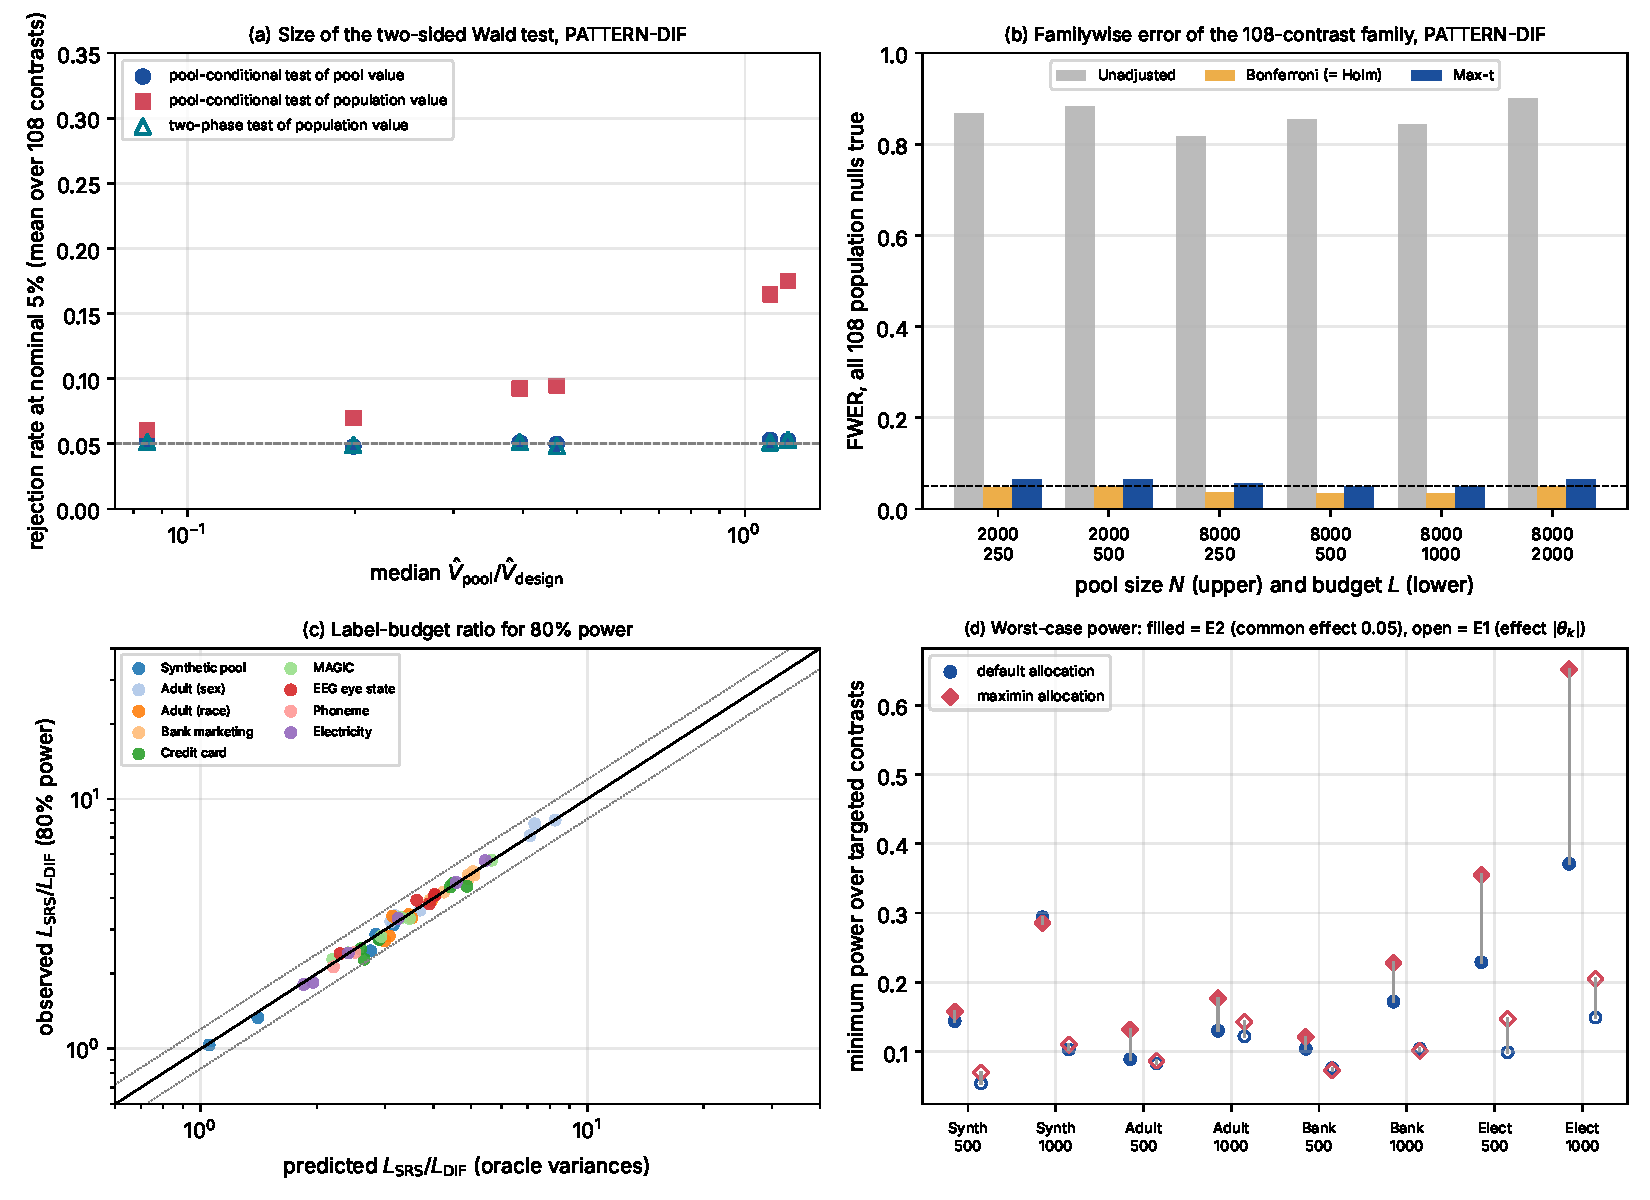
\includegraphics[width=\textwidth]{figures/testing_sim}
\caption{(a) Rejection rate at nominal $5\%$ (mean over $108$ contrasts) against the estimated ratio of pool to design variance. (b) FWER of the family in which all $108$ population hypotheses are true, by cell ($N$ above, $L$ below). (c) Predicted and observed $L_{\rm SRS}/L_{\rm DIF}$ at $80\%$ power, one point per contrast; dotted lines: $\pm20\%$. (d) Minimum simulated power over the targeted contrasts under the default and the maximin allocation (filled: E2, open: E1).}\label{fig:testing-sim}
\end{figure}

\paragraph{Limitations.} The nulls are exact only in the population and there are only $12$ of them, so the adjusted FWER with true nulls is conservative and the all-true family is the demanding check. There is one synthetic design and eleven real pools; the power study uses contrasts whose budgets fall in the grid, and the power-optimal allocation is evaluated with the true effect sizes and the proxy variance model. Max-$t$ uses an estimated correlation matrix of $108$ contrasts and is mildly anticonservative at small budgets. Further limitations are listed in Supplementary Section~\SIref{si:testing-sim}.

\section{Empirical study on eleven data settings}\label{sec:empirical}

\subsection{Data, models and protocol}
We use eleven settings built from ten public binary classification data sets available on OpenML (Table~\ref{tab:data}; details in Supplementary Section~\SIref{app:data}). In five settings the group is a protected attribute: sex or race in Adult, age below 30 in Bank Marketing, sex in the credit-card default data and race in the law-school admission data. In the other six the group is an arbitrary split of the first numeric feature at its median, removed from the features; these settings have no fairness meaning but cover a wider range of prediction structures. A twelfth candidate (Nomao) was excluded because its arbitrary group contains no positive instances.

Each data set is split once into a training part (60\%) and a pool (40\%); the Electricity data (45,312 rows) were first subsampled to 30,000, while Adult and Bank Marketing are used in full. Nine classifiers are trained on the training part with scikit-learn: logistic regression with default and with strong regularisation, decision trees of depth 3 and 12, a random forest, histogram gradient boosting, 25-nearest neighbours, Gaussian naive Bayes and a multilayer perceptron. Their predictions and predicted probabilities on the pool, together with the group attribute, are all the design uses. The pool labels play two roles: they answer label queries, and they define the true values of the estimands, so that the error of every estimate is known exactly.

For each setting and budget $L\in\{250,500,1000,2000\}$ with $L\le N/4$ (35 setting--budget cells), we draw 200 independent labelled samples under each design and compute the $3\binom{9}{2}=108$ comparison estimands of \eqref{eq:theta}. The efficiency of a design is the ratio of the mean squared error under SRS to that under the design, computed for each estimand and summarised by the median over estimands; an efficiency of 4 means that SRS needs about four times as many labels for the same accuracy. Estimands whose true value is identically degenerate in the pool (for example when no model pair disagrees in a group) are excluded; this affects 51 of 108 estimands in the law-school setting only. Efficiencies are computed over the samples in which both designs give finite estimates; SRS produced an undefined estimate (no sampled positive in a group) in at most 0.5\% of its samples and the stratified designs never did. The designs are those of Section~\ref{sec:design}: SRS, SRS-DIF, GROUP, GROUP-DIF, PATTERN (plain estimator) and the proposed PATTERN-DIF, together with a variant of PATTERN-DIF whose allocation uses the residual variances. SRS, GROUP and PATTERN use the same random seeds as the earlier plug-in study (\texttt{results/label\_efficiency.json}), so their samples coincide with it and their efficiencies agree except in law school, where that study used a different set of compared estimands. The code and all results are in the repository (\texttt{experiments/label\_efficiency\_dif.py}, \texttt{results/label\_efficiency\_dif.json}).

\begin{table}[t]\centering\small
\caption{Data settings. Pool: size of the held-out pool from which labels are drawn. $P_0,P_1$: positives in each group. Disagreement: share of pool instances on which two of the three most accurate models disagree, averaged over the three pairs. Groups marked ``arbitrary'' are median splits of a numeric feature.}\label{tab:data}
\begin{tabular}{lcrrrr}\toprule
Setting & Group & Pool $N$ & Positives $P_0$ & Positives $P_1$ & Disagreement \\\midrule
Adult (sex) & sex & 19537 & 3963 & 712 & 0.053 \\
Adult (race) & race & 19537 & 4249 & 426 & 0.047 \\
Bank marketing & age & 18085 & 1753 & 363 & 0.045 \\
Credit card & sex & 12000 & 1148 & 1506 & 0.030 \\
Law school & race & 8320 & 2038 & 640 & 0.000 \\
MAGIC & arbitrary & 7608 & 1084 & 1591 & 0.049 \\
EEG eye state & arbitrary & 5992 & 1183 & 1506 & 0.086 \\
Phoneme & arbitrary & 2162 & 388 & 247 & 0.095 \\
Spambase & arbitrary & 1841 & 490 & 235 & 0.043 \\
Churn & arbitrary & 2000 & 149 & 134 & 0.041 \\
Electricity & arbitrary & 12000 & 2582 & 2488 & 0.086 \\
\bottomrule\end{tabular}
\end{table}

\subsection{Efficiency}
Table~\ref{tab:efficiency} gives the efficiency of every design in every cell, Table~\ref{tab:decomposition} summarises it by budget and Figure~\ref{fig:efficiency} shows it as a function of the budget and of the disagreement rate. Across settings, the median efficiency of PATTERN-DIF relative to SRS is 5.8 at $L=250$ (eleven settings), 6.3 at $L=500$ (ten), 6.9 at $L=1000$ (eight) and 15.5 at $L=2000$ (six); without the degenerate law-school setting the medians are 5.5, 5.8, 6.0 and 9.4. SRS thus needs between five and sixteen times as many labels to match PATTERN-DIF, and the lowest efficiency in any cell outside law school is 3.5. The medians over settings rise with the budget partly because the set of settings changes (only the larger pools allow the larger budgets): on the seven non-degenerate settings that are present at $L=250$, 500 and 1000 the medians of PATTERN-DIF are 5.3, 5.3 and 6.0 (3.5, 3.8 and 4.4 for PATTERN). Within each of these seven settings the efficiency does increase with the budget (a median increase of 23\% from $L=250$ to $L=1000$), because a larger budget labels a larger share of the small disagreement strata, where the variance of the comparisons is concentrated. The increase is moderate except at $L=2000$, where the remaining settings are those with the largest pools and the strongest gains.

\paragraph{Where the gain comes from.} Table~\ref{tab:decomposition} separates the two ingredients, and the design is the larger. Under the difference estimator, moving from simple random sampling to the PATTERN strata multiplies the efficiency by 3.3 to 8.6 (PATTERN-DIF against SRS-DIF), and under the plain estimator by 3.7 to 7.3 (PATTERN against SRS). The estimator contributes 1.3 to 1.65 on top of the PATTERN design (PATTERN-DIF against PATTERN, better in 34 of 35 cells), but only 1.8 to 2.0 on top of simple random sampling (SRS-DIF against SRS). The two ingredients are complementary, and neither accounts for the whole gain. Stratifying by group alone gives almost no gain under the plain estimator (median 1.04 to 1.05 at the first three budgets and 1.25 at $L=2000$, where it is 1.0 without law school) and 2.1 to 2.7 with the difference estimator, which is essentially the value of the proxy correction. The variance of a contrast between two models is driven by the instances on which they disagree, and these are spread over both groups.

\paragraph{By estimand.} Efficiency differs by estimand. For PATTERN-DIF the medians over settings at the four budgets are 5.8, 5.3, 8.9 and 17.0 for $\theta^{\mathrm{TPR}}$, 7.6, 8.5, 8.4 and 20.6 for $\theta^{\mathrm{FPR}}$, and 3.5, 4.1, 4.4 and 5.7 for $\theta^{\mathrm{ERR}}$. The fairness contrasts gain more than the error contrast because they depend on the rarest cells (positives or negatives in the minority group). In Adult with race as the group, at $L=1000$, the efficiencies are 23.9 for $\theta^{\mathrm{TPR}}$, 20.6 for $\theta^{\mathrm{FPR}}$ and 3.7 for $\theta^{\mathrm{ERR}}$. For the pairs formed by the three most accurate models, the comparisons most likely to matter in practice, the median efficiency of PATTERN-DIF is 5.8, 6.8, 6.6 and 10.5 at the four budgets (3.3, 4.2, 3.9 and 6.2 for PATTERN).

\begin{figure}[t]\centering
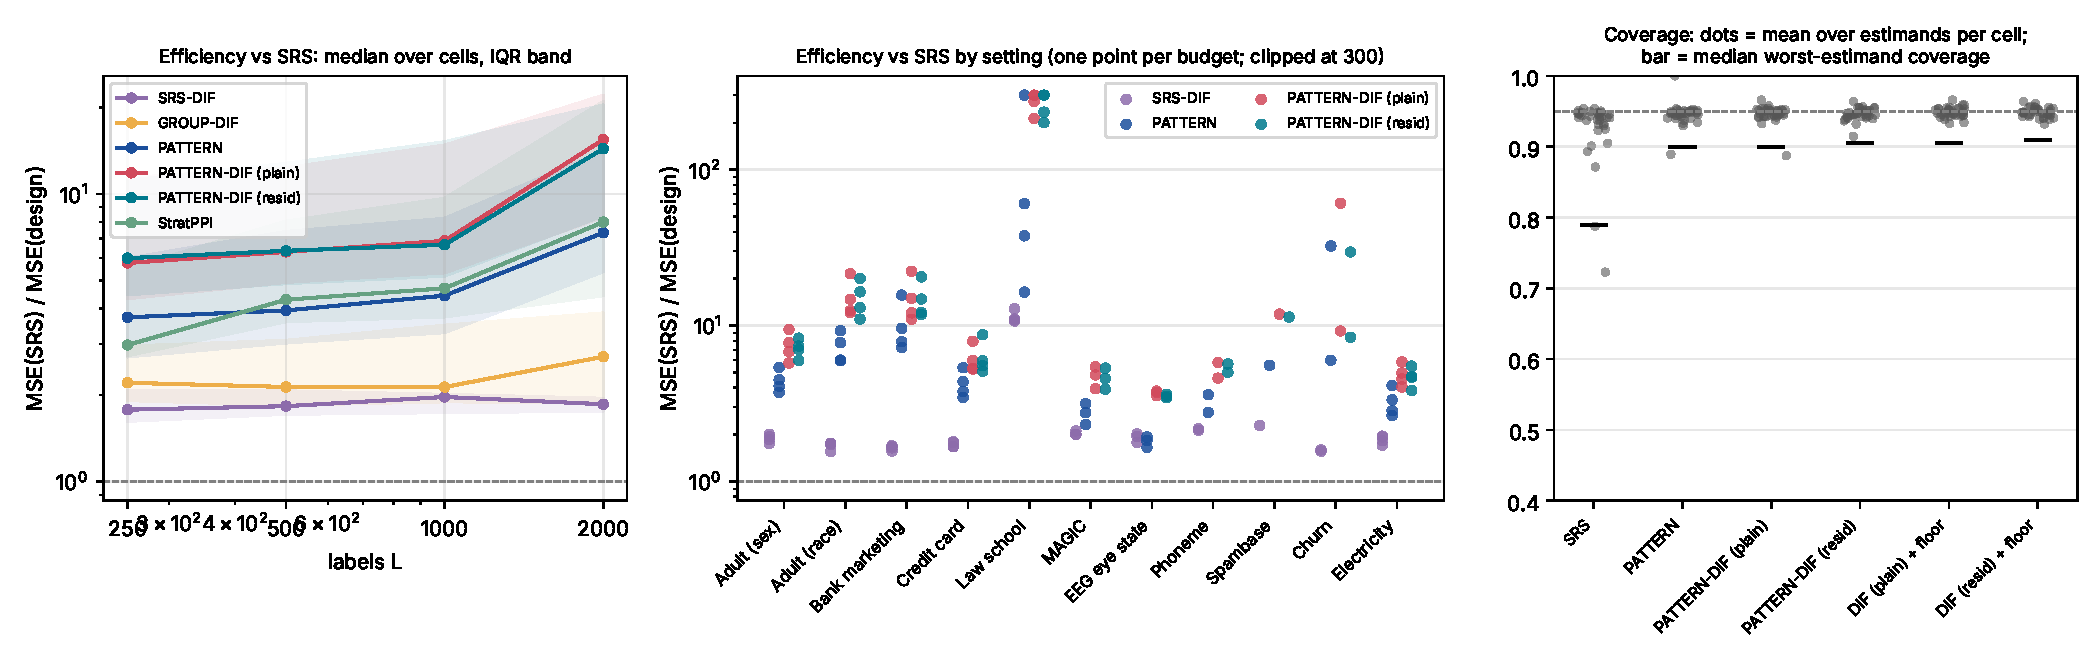
\includegraphics[width=\textwidth]{figures/efficiency_dif.pdf}
\caption{Efficiency of the designs relative to SRS (median over the comparison estimands) as a function of the label budget and of the disagreement rate; see Table~\ref{tab:efficiency} for the numbers.}\label{fig:efficiency}
\end{figure}

\begin{table}[t]\centering\small
\caption{Decomposition of the efficiency gain by budget (median over settings of the cell medians). Each row is a ratio of mean squared errors. ``DIF resid vs DIF plain'' compares the residual-variance allocation with the allocation used by default.}\label{tab:decomposition}
\begin{tabular}{lrrrr}\toprule
Step (MSE ratio) & $L=250$ & $L=500$ & $L=1000$ & $L=2000$ \\\midrule
SRS-DIF vs SRS & 1.78 & 1.83 & 1.97 & 1.86 \\
PATTERN vs SRS & 3.72 & 3.94 & 4.43 & 7.33 \\
PATTERN-DIF vs PATTERN & 1.65 & 1.54 & 1.51 & 1.31 \\
PATTERN-DIF vs SRS-DIF & 3.28 & 3.29 & 3.72 & 8.57 \\
PATTERN-DIF vs SRS & 5.76 & 6.29 & 6.87 & 15.5 \\
DIF resid vs DIF plain & 1.01 & 0.97 & 0.96 & 1.00 \\
\bottomrule\end{tabular}

\end{table}

\subsection{Efficiency and disagreement}
The gain is larger when the models disagree less (Figure~\ref{fig:efficiency}). The Spearman correlation between the disagreement rate of the three best models and the efficiency of PATTERN-DIF is $-0.58$ at $L=250$ (ten settings), $-0.53$ at $L=500$ (nine) and $-0.71$ at $L=1000$ (seven), excluding law school ($-0.68$, $-0.66$ and $-0.81$ with it). The three settings with the highest disagreement (EEG, electricity and phoneme, 8.6\% to 9.5\%) have the smallest gains, between 3.7 and 5.8 at $L=500$. The relation is inexact, since efficiency also depends on the size of the minority cells and on the magnitude of the contrasts (Section~\ref{sec:theory}; checked in Supplementary Section~\SIref{sec:simulation}).

Two settings are atypical. In the law-school data all nine models predict almost identically (the three best models disagree on fewer than 0.01\% of instances); the design then labels almost every disagreement instance and the contrasts are estimated nearly exactly, so the efficiency ratios (about 270 at $L=500$, 510 at $L=1000$ and above $10^{4}$ at $L=2000$) show only that SRS wastes labels on agreements. In the churn data (a pool of 2,000) the efficiency of PATTERN-DIF at $L=500$ is 61, driven by contrasts of false positive rates and of errors that are concentrated in very few instances.

\begin{table*}[p]\centering\footnotesize
\caption{Efficiency (ratio of mean squared errors, median over estimands) by setting and budget. DIF plain: PATTERN-DIF with the default allocation; DIF resid: with the residual-variance allocation; StratPPI: stratified prediction-powered inference (Section~\ref{sec:baselines}). ``vs PATTERN'': PATTERN-DIF relative to the plain estimator under the same design. The last three columns are the efficiencies of PATTERN-DIF by estimand type. Bold marks the best of the two PATTERN-DIF variants.}\label{tab:efficiency}
\begin{tabular}{lrrrrrrrr rrr}\toprule
Setting & $L$ & \multicolumn{6}{c}{Efficiency vs SRS} & vs PATTERN & \multicolumn{3}{c}{PATTERN-DIF (plain) by estimand} \\
 & & SRS-DIF & GROUP-DIF & PATTERN & DIF plain & DIF resid & StratPPI & DIF plain & $\theta^{TPR}$ & $\theta^{FPR}$ & $\theta^{ERR}$ \\\midrule
Adult (sex) & 250 & 1.75 & 2.20 & 3.72 & 5.76 & \textbf{5.98} & 3.28 & 1.37 & 8.68 & 7.59 & 3.50 \\
 & 500 & 1.86 & 1.95 & 4.08 & 6.80 & \textbf{7.02} & 4.07 & 1.49 & 9.30 & 8.20 & 3.83 \\
 & 1000 & 2.01 & 1.91 & 4.49 & \textbf{7.76} & 7.39 & 4.71 & 1.51 & 11.8 & 8.75 & 4.28 \\
 & 2000 & 1.94 & 1.87 & 5.39 & \textbf{9.42} & 8.30 & 5.54 & 1.32 & 11.7 & 11.8 & 5.03 \\
\addlinespace
Adult (race) & 250 & 1.56 & 3.31 & 5.96 & \textbf{12.1} & 11.0 & 5.46 & 1.65 & 18.1 & 15.4 & 2.96 \\
 & 500 & 1.73 & 3.33 & 6.02 & 12.4 & \textbf{13.0} & 6.95 & 1.44 & 17.5 & 14.9 & 3.44 \\
 & 1000 & 1.76 & 3.36 & 7.78 & 14.7 & \textbf{16.5} & 8.52 & 1.48 & 23.9 & 20.6 & 3.70 \\
 & 2000 & 1.75 & 3.52 & 9.28 & \textbf{21.5} & 20.0 & 10.4 & 1.30 & 37.5 & 29.3 & 4.36 \\
\addlinespace
Bank marketing & 250 & 1.57 & 3.84 & 7.22 & 11.0 & \textbf{11.8} & 7.80 & 1.44 & 11.0 & 18.6 & 5.05 \\
 & 500 & 1.64 & 3.99 & 7.87 & 12.1 & \textbf{12.1} & 10.3 & 1.45 & 12.1 & 24.7 & 6.31 \\
 & 1000 & 1.67 & 3.90 & 9.60 & \textbf{15.0} & 14.8 & 13.1 & 1.43 & 15.6 & 38.9 & 6.56 \\
 & 2000 & 1.69 & 3.97 & 15.7 & 22.3 & 20.5 & \textbf{24.5} & 1.32 & 22.3 & 79.9 & 9.18 \\
\addlinespace
Credit card & 250 & 1.67 & 1.86 & 3.45 & \textbf{5.31} & 5.09 & 2.58 & 1.26 & 3.55 & 7.18 & 4.27 \\
 & 500 & 1.80 & 1.81 & 3.79 & 5.26 & \textbf{5.53} & 3.52 & 1.29 & 4.81 & 7.84 & 4.30 \\
 & 1000 & 1.67 & 1.68 & 4.37 & \textbf{5.98} & 5.94 & 3.71 & 1.42 & 5.90 & 8.01 & 5.00 \\
 & 2000 & 1.78 & 1.91 & 5.36 & 7.93 & \textbf{8.72} & 4.06 & 1.20 & 5.43 & 10.5 & 6.32 \\
\addlinespace
Law school & 250 & 10.9 & 22.2 & 16.4 & \textbf{$>$100} & $>$100 & 31.8 & 10.7 & $>$100 & $>$100 & $>$100 \\
 & 500 & 12.8 & 19.7 & 37.6 & \textbf{$>$100} & $>$100 & 52.4 & 9.46 & $>$100 & $>$100 & $>$100 \\
 & 1000 & 11.0 & 21.4 & 60.4 & \textbf{$>$100} & $>$100 & 78.4 & 8.26 & $>$100 & $>$100 & $>$100 \\
 & 2000 & 10.7 & 20.4 & \textbf{$>$100} & $>$100 & $>$100 & $>$100 & 0.00 & $>$100 & $>$100 & $>$100 \\
\addlinespace
MAGIC & 250 & 2.01 & 1.98 & 2.32 & \textbf{3.93} & 3.90 & 2.71 & 1.65 & 3.89 & 5.30 & 3.06 \\
 & 500 & 2.11 & 2.26 & 2.76 & \textbf{4.82} & 4.57 & 3.81 & 1.71 & 4.89 & 5.94 & 3.27 \\
 & 1000 & 2.01 & 2.10 & 3.16 & \textbf{5.43} & 5.33 & 4.69 & 1.61 & 4.73 & 6.75 & 4.60 \\
\addlinespace
EEG eye state & 250 & 1.78 & 1.96 & 1.65 & \textbf{3.55} & 3.51 & 2.71 & 1.93 & 3.80 & 4.06 & 2.98 \\
 & 500 & 1.94 & 2.00 & 1.83 & \textbf{3.73} & 3.44 & 3.33 & 1.82 & 4.23 & 3.99 & 3.15 \\
 & 1000 & 2.02 & 2.16 & 1.93 & \textbf{3.80} & 3.61 & 3.68 & 1.91 & 4.06 & 4.86 & 3.04 \\
\addlinespace
Phoneme & 250 & 2.13 & 2.29 & 2.77 & 4.60 & \textbf{5.02} & 2.98 & 1.77 & 4.68 & 6.74 & 3.19 \\
 & 500 & 2.18 & 2.41 & 3.60 & \textbf{5.79} & 5.67 & 4.51 & 1.78 & 5.66 & 8.71 & 4.36 \\
\addlinespace
Spambase & 250 & 2.29 & 2.61 & 5.55 & \textbf{11.8} & 11.3 & 5.56 & 2.19 & 16.1 & 20.0 & 5.69 \\
\addlinespace
Churn & 250 & 1.56 & 1.49 & 5.99 & \textbf{9.22} & 8.41 & 2.96 & 1.42 & 5.77 & 10.3 & 9.48 \\
 & 500 & 1.59 & 1.78 & 32.4 & \textbf{60.8} & 29.6 & 8.42 & 1.28 & 4.46 & 70.6 & 77.1 \\
\addlinespace
Electricity & 250 & 1.83 & 1.84 & 2.65 & \textbf{4.04} & 3.83 & 2.76 & 1.63 & 4.88 & 5.26 & 2.97 \\
 & 500 & 1.71 & 1.78 & 2.84 & 4.54 & \textbf{4.66} & 3.40 & 1.59 & 4.82 & 5.42 & 3.20 \\
 & 1000 & 1.93 & 1.85 & 3.34 & \textbf{4.97} & 4.72 & 3.74 & 1.51 & 5.01 & 6.27 & 4.07 \\
 & 2000 & 1.95 & 1.85 & 4.12 & \textbf{5.85} & 5.49 & 3.92 & 1.44 & 5.54 & 8.34 & 5.12 \\
\bottomrule\end{tabular}

\end{table*}

\subsection{Inference and decisions}
Table~\ref{tab:inference} reports the coverage of nominal 95\% intervals. The mean coverage of the PATTERN-DIF intervals is 0.940 at $L=250$, 0.946 at $L=500$ and between 0.950 and 0.952 at larger budgets; for PATTERN with the plain estimator it is 0.938, 0.944, 0.950 and 0.956. Under SRS it is 0.911 to 0.942, and the worst-covered estimand has coverage as low as 0.10 at $L=250$, because SRS samples often contain no disagreement instance in a small cell and then give a zero standard error. The worst-covered estimand under PATTERN-DIF has coverage 0.59 at $L=250$ (in law school), 0.84 at $L=500$ and 0.89 to 0.90 at larger budgets. The intervals are therefore adequate on average from 250 labels on, and for every estimand from about 1,000 labels on (worst-estimand coverage 0.89 to 0.90, about the minimum that chance alone gives over 108 estimands with 200 replicates). They fail in small cells at small budgets, where a stratum in which every sampled label is the same gives a variance estimate of exactly zero. A safeguard that replaces the zero variance of such a stratum by its variance under the proxy (a ``variance floor'', Section~\ref{sec:ablations}) raises the worst-estimand coverage at $L=250$ from 0.59 to 0.82 and keeps the mean at 0.946; a more conservative version raises the mean to 0.98. The floor was designed after seeing this failure on these pools, so the improvement is in-sample. At small budgets we report both the plain Wald and the floor intervals.

\begin{table*}[t]\centering\small
\caption{Quality of inference by budget. Mean: coverage of nominal 95\% intervals averaged over estimands and cells; worst: the lowest coverage of any estimand in any cell. ``+ floor'': Wald intervals with the zero-variance safeguard. Fail: largest share of samples with an undefined estimate (SRS only).}\label{tab:inference}
\resizebox{\textwidth}{!}{\begin{tabular}{rrrrrrrrrrrrrrrrr}\toprule
$L$ & Cells & \multicolumn{2}{c}{SRS} & \multicolumn{2}{c}{PATTERN} & \multicolumn{2}{c}{PATTERN-DIF (plain)} & \multicolumn{2}{c}{PATTERN-DIF (resid)} & \multicolumn{2}{c}{DIF (plain) + floor} & \multicolumn{2}{c}{DIF (resid) + floor} & \multicolumn{2}{c}{PATTERN + floor} & Fail \\
 & & mean & worst & mean & worst & mean & worst & mean & worst & mean & worst & mean & worst & mean & worst & (max) \\\midrule
250 & 11 & 0.911 & 0.10 & 0.938 & 0.53 & 0.940 & 0.59 & 0.943 & 0.69 & 0.946 & 0.82 & 0.948 & 0.85 & 0.963 & 0.90 & 0.005 \\
500 & 10 & 0.923 & 0.28 & 0.944 & 0.82 & 0.946 & 0.84 & 0.944 & 0.85 & 0.948 & 0.84 & 0.945 & 0.85 & 0.959 & 0.89 & 0.000 \\
1000 & 8 & 0.938 & 0.71 & 0.950 & 0.89 & 0.952 & 0.90 & 0.949 & 0.90 & 0.952 & 0.90 & 0.950 & 0.90 & 0.959 & 0.91 & 0.000 \\
2000 & 6 & 0.942 & 0.53 & 0.956 & 0.89 & 0.950 & 0.89 & 0.952 & 0.90 & 0.950 & 0.89 & 0.952 & 0.90 & 0.957 & 0.89 & 0.000 \\
\bottomrule\end{tabular}}

\end{table*}

\subsection{Repeated train/pool splits}\label{sec:splits}

All earlier results use one train/pool split and one set of nine fitted models per setting. To measure how much the efficiency depends on the split, we repeated the main study for the six largest settings (Adult with sex and with race as the group, Bank marketing, credit-card default, MAGIC and Electricity; pools of $7608$ to $19537$ instances) on three new splits, with seeds $1$, $2$ and $3$. For each split the nine models were refitted on the new $60\%$ training part (the learners' own random seeds were not changed, so the variation comes from the data split and the refit), the pool is the new $40\%$ held-out part, and the protocol of Section~\ref{sec:empirical} was run for SRS, GROUP, PATTERN and PATTERN-DIF with $L\in\{500,1000\}$ and $R=100$ replicates per cell. The original split (seed $0$, $R=200$) is included as the fourth value. The code is \texttt{experiments/label\_efficiency\_splits.py}; the numbers are in \texttt{results/label\_efficiency\_splits.json} and \texttt{results/label\_\allowbreak efficiency\_\allowbreak splits\_\allowbreak summary.json}. Efficiency is defined as before, the median over contrasts of the ratio of mean squared errors against SRS, computed on the pool of each split.

\begin{table}[t]
\centering\small
\caption{Efficiency of PATTERN-DIF against SRS (ratio of mean squared errors) on four train/pool splits. Split 0 is the original one. Mean, standard deviation and range are over the four splits. The last rows give the median over the six settings. Source: \texttt{results/label\_efficiency\_splits.json}.}\label{tab:split-main}
\begin{tabular}{lrrrrrrrr}\toprule
Setting & $L$ & split 0 & split 1 & split 2 & split 3 & Mean & SD & Range \\\midrule
Adult (sex) & 500 & 6.8 & 7.8 & 6.8 & 8.1 & 7.4 & 0.7 & 6.8--8.1 \\
 & 1000 & 7.8 & 7.3 & 7.2 & 7.8 & 7.5 & 0.3 & 7.2--7.8 \\
\addlinespace
Adult (race) & 500 & 12.4 & 10.6 & 12.8 & 14.6 & 12.6 & 1.6 & 10.6--14.6 \\
 & 1000 & 14.7 & 14.9 & 16.4 & 15.6 & 15.4 & 0.8 & 14.7--16.4 \\
\addlinespace
Bank marketing & 500 & 12.1 & 11.6 & 12.4 & 11.6 & 11.9 & 0.4 & 11.6--12.4 \\
 & 1000 & 15.0 & 15.2 & 13.2 & 12.7 & 14.0 & 1.2 & 12.7--15.2 \\
\addlinespace
Credit card & 500 & 5.3 & 5.6 & 6.1 & 6.7 & 5.9 & 0.6 & 5.3--6.7 \\
 & 1000 & 6.0 & 6.5 & 7.9 & 6.7 & 6.8 & 0.8 & 6.0--7.9 \\
\addlinespace
MAGIC & 500 & 4.8 & 4.5 & 5.4 & 5.0 & 4.9 & 0.4 & 4.5--5.4 \\
 & 1000 & 5.4 & 5.2 & 5.2 & 5.8 & 5.4 & 0.3 & 5.2--5.8 \\
\addlinespace
Electricity & 500 & 4.5 & 4.3 & 4.2 & 4.3 & 4.3 & 0.1 & 4.2--4.5 \\
 & 1000 & 5.0 & 5.3 & 4.5 & 4.9 & 4.9 & 0.3 & 4.5--5.3 \\
\addlinespace
Median over settings & 500 & 6.0 & 6.7 & 6.5 & 7.4 & \multicolumn{3}{c}{} \\
Median over settings & 1000 & 6.9 & 6.9 & 7.6 & 7.3 & \multicolumn{3}{c}{} \\
\bottomrule\end{tabular}

\end{table}

\begin{figure}[t]
\centering
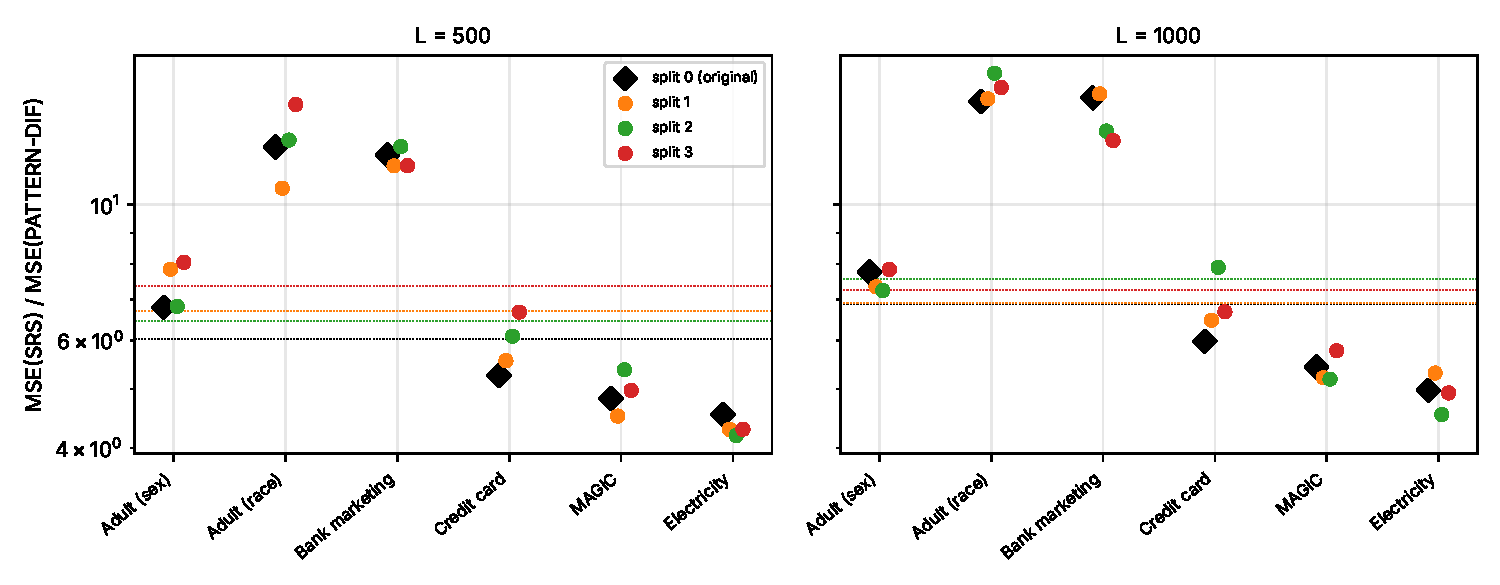
\includegraphics[width=\textwidth]{figures/splits_efficiency}
\caption{Efficiency of PATTERN-DIF against SRS by setting and split. The diamond is the original split. Dotted lines are the medians over the six settings for each split.}\label{fig:split-eff}
\end{figure}

Table~\ref{tab:split-main} and Figure~\ref{fig:split-eff} show that the efficiency is stable across splits relative to its variation across settings, which ranges from $4.9$ (Electricity, mean over the four splits) to $15.4$ (Adult with race) at $L=1000$. The median over settings of the coefficient of variation across the four splits is $0.07$ and the median ratio of the largest to the smallest split value is $1.18$. The largest spreads are Adult (race) at $L=500$ (from $10.6$ to $14.6$) and Credit card at $L=1000$ ($6.0$ to $7.9$). Part of this spread is Monte Carlo error, since each value rests on $100$ replicates ($200$ for split $0$). Adult (race) and Bank have the highest efficiency and Electricity and MAGIC the lowest in every split and at both budgets. The efficiency of PATTERN-DIF is at least $4.2$ in all $48$ cell-split values.

The median over the six settings is $6.0$, $6.7$, $6.5$ and $7.4$ at $L=500$ for splits $0$ to $3$, and $6.9$, $6.9$, $7.6$ and $7.3$ at $L=1000$. The original split gives the lowest median of the four at both budgets (at $L=1000$ only marginally below split~1), so the choice of split does not flatter the headline numbers of the main study in these settings. Pooling the four splits, the median is $6.7$ at $L=500$ and $7.3$ at $L=1000$ against $6.0$ and $6.9$ for split $0$ alone, a difference of at most about $12\%$ on a factor of 6 to 7. Coverage is unaffected: the mean coverage of the PATTERN-DIF intervals is $0.948$ to $0.951$ on every split ($0.950$ overall), against $0.939$ to $0.941$ for SRS with the plug-in estimator. The worst contrast in any split has coverage $0.84$ to $0.88$ for PATTERN-DIF; with $100$ replicates per cell the Monte Carlo standard error of one coverage is $0.02$, so these worst values are partly noise.

These results have three limits. Four splits in total (three new) are far fewer than the $20$ that a full study of between-split variation would use, so the spread in Table~\ref{tab:split-main} is a rough indication only. Only the six largest settings were repeated, so the median over all eleven settings of the main study is not recomputed. The nine models share the same families in every split, and the splits do not change the learner seeds or the groups, so variation from other hyperparameters or model families is not covered.

\subsection{Target of inference: the pool or the population}\label{sec:population}

The intervals of Section~\ref{sec:design} cover the contrast computed on the pool, $\theta_U=f(T_U)$. If the pool is itself a sample of $N$ units from a deployment population, the quantity of interest is the population contrast $\theta_{\rm pop}=\tilde f(\tau)$, $\tau=\mathrm E\,t_i(Y_i)$, and the pool-conditional interval ignores the pool's sampling error. Write $\hat\theta=f(T_{\rm dif})$ for the unchanged estimator. Then
\[
\hat\theta-\theta_{\rm pop}=\underbrace{f(T_{\rm dif})-f(T_U)}_{\text{design error}}+\underbrace{f(T_U)-f(N\tau)}_{\text{pool error}} .
\]
Given the pool, the first term has mean zero to first order and variance $V_{\rm design}=\sum_h N_h^2(1-n_h/N_h)S_h^2(e)/n_h$, the quantity estimated in Section~\ref{sec:design}. The second term is, to first order, a sum of $N$ independent influence values, so the two terms are uncorrelated and
\begin{equation}\label{eq:pop-variance}
\begin{gathered}
V_{\rm total}=\mathrm E\,V_{\rm design}+V_{\rm pool},\\
V_{\rm pool}=N\,\mathrm{Var}(z_i),\qquad z_i=\mathbf b^{\top}\bigl(t_i(Y_i)-\tau\bigr),
\end{gathered}
\end{equation}
with $\mathbf b=\nabla f(N\tau)$ the gradient on the scale of totals. This is the two-phase decomposition of \citet{sarndal1987}. The influence value $z_i$ is that of the full-label plug-in contrast, not the residual $e_i$ of the difference estimator: the proxy removes variance from the labelled part of the error but cannot remove the variation of $Y$ across units of the population, so, to first order, $V_{\rm pool}$ is the same for every labelling design and every proxy.

Since the labelled sample is a stratified sample of the pool, $V_{\rm pool}$ is estimated with the weights $w_i=N_h/n_h$:
\[
\begin{gathered}
\hat V_{\rm pool}=\sum_{i\in s}w_i\,(\hat z_i-\bar z)^2,\\
\bar z=\frac1N\sum_{i\in s}w_i\hat z_i,\qquad \hat z_i=\hat{\mathbf b}^{\top}t_i(Y_i),
\end{gathered}
\]
with $\hat{\mathbf b}=\nabla f(T_{\rm dif})$, and the two-phase interval is $\hat\theta\pm1.96\sqrt{\hat V_{\rm design}+\hat V_{\rm pool}}$. The derivation is in \texttt{docs/two\_phase\_note.md} and the code in \texttt{tcs/labeling\_two\_phase.py}. Let $\varpi=V_{\rm pool}/V_{\rm design}$. It is of order $L\,\mathrm{Eff}/N$, where $\mathrm{Eff}$ is the efficiency of the design against SRS, so it grows with the budget and the efficiency and shrinks with the pool size. With correct $V_{\rm design}$ and normal errors the pool-conditional interval has coverage about $2\Phi(1.96/\sqrt{1+\varpi})-1$ of the population contrast, which is $0.93$ at $\varpi=0.2$, $0.83$ at $\varpi=1$ and $0.67$ at $\varpi=3$. Efficiency changes in the same way: the pool term is shared by SRS and PATTERN-DIF, so against the population contrast the MSE ratio is $(\mathrm{Eff}+\varpi)/(1+\varpi)$, with $\varpi$ evaluated for PATTERN-DIF, rather than $\mathrm{Eff}$. For $\mathrm{Eff}=6$ and $\varpi=1.5$ this is $3$. This follows arithmetically from \eqref{eq:pop-variance}; it is not an estimate from the earlier experiments.

\subsubsection*{Experiment}
We checked the two intervals against population values in a synthetic setting; the real data sets are not used. The population is the generative model of the non-smooth simulation (five Gaussian covariates, a group with prevalence $0.3$, a logistic label model) with nine fixed scoring rules, so there are $36$ pairs and $108$ contrasts, $\theta^{TPR}$, $\theta^{FPR}$ and $\theta^{ERR}$. Population values were computed on $6\times10^{6}$ draws. For every replicate a new pool of $N\in\{2000,8000,20000\}$ units is drawn and then a PATTERN-DIF sample (PATTERN strata, plain allocation, difference estimator) of $L\in\{250,500,1000,2000\}$ labels ($L\le N/4$; ten cells), with the mean-probability proxy; $R=300$ replicates per cell. Table~\ref{tab:pop-check} and Figure~\ref{fig:pop-check} give the coverage, averaged over the $108$ contrasts and for the worst contrast, together with the median over contrasts of $\hat V_{\rm pool}/\hat V_{\rm design}$ (source: \texttt{results/two\_phase\_check.json}).

\begin{table}[t]
\centering\small
\caption{Coverage of the population contrast (nominal $0.95$) over $108$ contrasts, $R=300$ pools per row. $V_{\rm pool}/V_{\rm des}$ is the median over contrasts of the estimated ratio. The last column is the coverage of the pool value by the pool-conditional interval. Source: \texttt{results/two\_phase\_check.json}.}\label{tab:pop-check}
\begin{tabular}{rr r rr rr r}\toprule
 & & & \multicolumn{2}{c}{Pool-conditional} & \multicolumn{2}{c}{Two-phase} & Pool value \\
$N$ & $L$ & $V_{\mathrm{pool}}/V_{\mathrm{des}}$ & mean & worst & mean & worst & (pool-cond.) mean \\\midrule
2{,}000 & 250 & 0.50 & 0.899 & 0.86 & 0.949 & 0.92 & 0.949 \\
 & 500 & 1.51 & 0.809 & 0.72 & 0.952 & 0.92 & 0.948 \\
\addlinespace
8{,}000 & 250 & 0.11 & 0.940 & 0.91 & 0.951 & 0.92 & 0.952 \\
 & 500 & 0.25 & 0.921 & 0.87 & 0.947 & 0.90 & 0.948 \\
 & 1000 & 0.58 & 0.889 & 0.83 & 0.950 & 0.92 & 0.945 \\
 & 2000 & 1.57 & 0.792 & 0.64 & 0.949 & 0.92 & 0.953 \\
\addlinespace
20{,}000 & 250 & 0.04 & 0.940 & 0.90 & 0.945 & 0.91 & 0.945 \\
 & 500 & 0.09 & 0.942 & 0.90 & 0.952 & 0.91 & 0.953 \\
 & 1000 & 0.20 & 0.928 & 0.89 & 0.947 & 0.92 & 0.949 \\
 & 2000 & 0.44 & 0.903 & 0.83 & 0.949 & 0.91 & 0.949 \\
\bottomrule\end{tabular}

\end{table}

\begin{figure}[t]
\centering
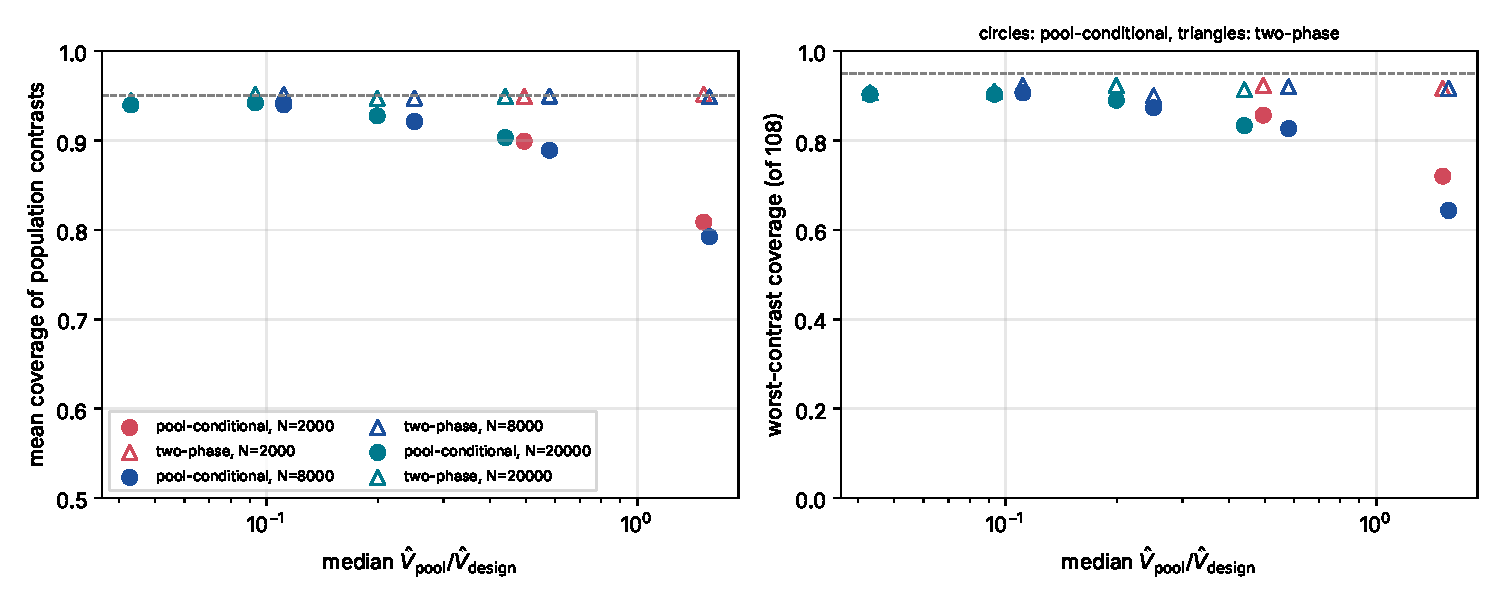
\includegraphics[width=\textwidth]{figures/two_phase_check}
\caption{Coverage of the population contrasts against the median ratio $\hat V_{\rm pool}/\hat V_{\rm design}$, one point per $(N,L)$ cell. Left: mean over the $108$ contrasts. Right: worst contrast. Circles: pool-conditional intervals, triangles: two-phase intervals; colours give $N$.}\label{fig:pop-check}
\end{figure}

The pool-conditional interval keeps its coverage of the pool value (mean $0.945$ to $0.953$ in all ten cells), so the earlier results are not affected. Against the population contrast its mean coverage falls with $\varpi$: $0.94$ when $\varpi\le0.11$, $0.90$ to $0.93$ for $\varpi$ between $0.2$ and $0.5$, $0.89$ at $\varpi=0.58$ and $0.79$ to $0.81$ at $\varpi\approx1.5$ (the cells $N=2000,L=500$ and $N=8000,L=2000$), where the worst contrast is covered in $0.72$ and $0.64$ of the replicates. This is close to the value the formula predicts. The two-phase interval has mean coverage $0.945$ to $0.952$ in every cell and worst-contrast coverage $0.90$ to $0.92$. The worst of $108$ contrasts with $300$ replicates has a Monte Carlo standard error of $0.013$, so the worst value is expected to lie near $0.92$ even for exact intervals. We do not read the remaining gap as a failure, but the experiment cannot exclude a small one. The cost is width: the two-phase interval is $2\%$ to $10\%$ wider when $\varpi\le0.2$, $12\%$ wider at $\varpi=0.25$ and $21\%$ to $71\%$ wider when $\varpi\ge0.44$ (median width over contrasts).

\subsubsection*{When the pool term matters}
It does not matter when $N$ is large relative to the budget: at $N=20000$ and $L\le500$, $\varpi\le0.09$ and the two intervals are nearly the same. It matters when the labelled fraction is not small, as in the small pools of the empirical study (about $2000$ to $20000$ instances, budgets up to $2000$). The empirical MSE of $\hat\theta$ around the population contrast is $1.04$ to $2.6$ times its MSE around the pool contrast in these cells. Three limits apply. The simulation is stylised: the pool is an independent sample of the population and the models are fixed and independent of the pool. With real data the deployment population is unknown, the pool may be a convenience sample, and the two-phase interval is only as good as the assumption that the pool is representative. If the pool is the whole deployment set, the pool-conditional interval is the right one and the two-phase interval is conservative. The gain of PATTERN-DIF over SRS also shrinks for the population target, as shown above, although the ranking of designs does not change. We did not run the full pipeline (training, pooling, labelling) against full-data references on the OpenML data; the known population above isolates the pool-sampling term.

\section{Comparison with existing labelling designs}\label{sec:baselines}

PATTERN-DIF combines four ingredients that are each known: sampling where models disagree, stratification on a model-based proxy with Neyman-type allocation, design-based ratio estimation and a model-assisted (difference) estimator. This section asks whether natural alternatives built from one or two of these ingredients already do as well. The study was run before the final form of the method was fixed. Its PATTERN-DIF variant (B5, $\lambda=1$) is the same estimator as the main method, but the samples differ from those of Section~\ref{sec:empirical} (different random seeds). Values differ between the two studies by a median of about 5\% per cell (up to 27\% in single cells, law school excluded) and the medians over settings by up to 14\% (PATTERN-DIF at $L=250$: 6.6 here, 5.8 in Section~\ref{sec:empirical}). The abstract and the main results use the study of Section~\ref{sec:empirical}. We ran the baselines and SRS and PATTERN on the eleven settings of Section~\ref{sec:empirical}, at $L\in\{250,500,1000,2000\}$ with $L\le N/4$ (35 setting--budget cells) and $R=200$ replications per cell. To isolate the effect of labelling and estimation, every method estimates the same totals $T$, maps them through the same $\hat\theta=f(\hat T)$ to the same 108 comparison estimands, uses the same proxy $\pi_i$ and allocation weights where it has any, and reports 95\% Wald intervals; the budget is counted in distinct labelled instances. Estimands that every design estimates exactly are excluded (51 of 108 in Law school, none elsewhere). Full definitions are in Supplementary Section~\SIref{si:baselines}.

\paragraph{Baselines.} B1 is importance sampling for active comparison \citep{sawade2012active}: draws with replacement from an instrumental distribution that is proportional to the root of the proxy-expected squared influence, adapted here to TPR and FPR gaps, with self-normalised totals. B2 stratifies on the proxy score (group $\times$ quantile bins of $\pi_i$; Score-10 and Score-5) with the same proxy-Neyman allocation as PATTERN \citep{bennett2010online,kumar2018classifier}, so it differs from PATTERN only in the strata. B3 is a disagreement-focused two-phase design (Dis-25, Dis-50): a simple random first phase of $L/4$ or $L/2$ labels, then a simple random sample of the disagreement set for the rest \citep{sawade2012active,musgrove2023discordant}. B4 is prediction-powered inference: PPI with $\lambda=1$ \citep{angelopoulos2023ppi}, PPI++ with a tuned $\lambda$ \citep{angelopoulos2026ppipp} and StratPPI, which applies PPI++ within proxy strata with a Neyman-type allocation \citep{fisch2024stratppi}. B5 is the proposed method: the PATTERN design with the stratified difference estimator ($\lambda=1$, PATTERN-DIF), and a tuned-weight variant (PATTERN-PPI).

\begin{table}[t]\centering\small
\caption{Baselines by label budget $L$ (number of settings in brackets). Efficiency: ratio of mean squared errors, median over the non-degenerate comparison estimands within a setting, then median over settings; ``vs SRS'' is MSE(SRS)/MSE(method), ``vs PATTERN'' is MSE(PATTERN)/MSE(method), so values above 1 favour the method. Coverage: nominal 95\% Wald intervals, mean over estimands and settings; ``worst'': lowest single-estimand coverage over all settings and budgets. $R=200$ replications per setting and budget. Source: \texttt{results/label\_baselines.json}.}\label{tab:base-budget}
\setlength{\tabcolsep}{3.5pt}
\resizebox{\textwidth}{!}{\begin{tabular}{lrrrrrrrrrrr}\toprule
 & \multicolumn{2}{c}{$L=250$ (11)} & \multicolumn{2}{c}{$L=500$ (10)} & \multicolumn{2}{c}{$L=1000$ (8)} & \multicolumn{2}{c}{$L=2000$ (6)} & \multicolumn{3}{c}{All $(s,L)$} \\
\cmidrule(lr){2-3} \cmidrule(lr){4-5} \cmidrule(lr){6-7} \cmidrule(lr){8-9} \cmidrule(lr){10-12}
Method & vs SRS & vs PAT. & vs SRS & vs PAT. & vs SRS & vs PAT. & vs SRS & vs PAT. & Cover. & Worst & ms \\ \midrule
SRS & 1 & 0.27 & 1 & 0.25 & 1 & 0.23 & 1 & 0.14 & 0.925 & 0.16 & 8 \\
PATTERN & 3.75 & 1 & 3.95 & 1 & 4.35 & 1 & 7.43 & 1 & 0.947 & 0.52 & 8 \\
IS (B1) & 3.09 & 0.79 & 2.77 & 0.74 & 3.48 & 0.67 & 4.30 & 0.54 & 0.950 & 0.60 & 9 \\
Score-10 (B2) & 1.45 & 0.40 & 2.09 & 0.52 & 2.24 & 0.56 & 4.16 & 0.50 & 0.941 & 0.17 & 8 \\
Score-5 (B2) & 1.97 & 0.54 & 2.24 & 0.57 & 2.15 & 0.52 & 3.18 & 0.43 & 0.943 & 0.37 & 8 \\
Dis-25 (B3) & 2.25 & 0.42 & 2.27 & 0.55 & 2.04 & 0.35 & 2.48 & 0.26 & 0.942 & 0.45 & 9 \\
Dis-50 (B3) & 1.84 & 0.43 & 1.94 & 0.37 & 1.68 & 0.34 & 1.93 & 0.25 & 0.940 & 0.36 & 9 \\
PPI (B4) & 1.82 & 0.49 & 1.82 & 0.47 & 1.86 & 0.44 & 1.81 & 0.27 & 0.940 & 0.27 & 34 \\
PPI++ (B4) & 2.10 & 0.49 & 1.97 & 0.48 & 1.93 & 0.44 & 1.89 & 0.27 & 0.929 & 0.16 & 49 \\
StratPPI (B4) & 3.07 & 1.01 & 4.45 & 1.12 & 4.58 & 1.08 & 8.50 & 0.83 & 0.924 & 0.14 & 44 \\
\midrule \multicolumn{12}{l}{\emph{Extension (B5): PATTERN sample, model-assisted estimator}} \\
PATTERN-DIF (B5) & 6.57 & 1.63 & 6.23 & 1.48 & 6.64 & 1.48 & 15.5 & 1.32 & 0.946 & 0.64 & 35 \\
PATTERN-PPI (B5) & 6.71 & 1.68 & 6.37 & 1.55 & 6.83 & 1.54 & 15.5 & 1.33 & 0.929 & 0.20 & 51 \\
\bottomrule\end{tabular}}\end{table}


\paragraph{Results.} Table~\ref{tab:base-budget} summarises all methods by budget. PATTERN is the most efficient of the designs that use the same plain estimator as SRS (B1 to B3) at every budget: its median efficiency against SRS is 3.75, 3.95, 4.35 and 7.43 at $L=250,500,1000,2000$. It is not the most efficient method overall: StratPPI, which combines proxy strata with a model-assisted estimator, matches or exceeds it in the paired medians at $L=250$, 500 and 1000 (ratios 1.01, 1.12, 1.08) and has the higher median efficiency against SRS at $L=500$, 1000 and 2000 (4.45, 4.58, 8.50), and the extensions B5, which add the same kind of correction to the PATTERN sample, beat both. Among the competing designs the closest are importance sampling (B1: 3.09, 2.77, 3.48, 4.30 against SRS; 0.54--0.79 of PATTERN) and StratPPI (B4: 3.07, 4.45, 4.58, 8.50; 1.01, 1.12, 1.08, 0.83 of PATTERN). Proxy-score strata alone (B2) reach 1.45--4.16 against SRS, the disagreement-only designs (B3) 1.7--2.5 and PPI/PPI++ with simple random labels 1.8--2.1, all clearly below PATTERN (medians 0.25--0.57 of its efficiency). PPI and PPI++ with SRS labels barely move with $L$: they use the proxy but not the fact that the numerators vanish where models agree. The model-assisted extensions improve on PATTERN in every cell except Law school at $L=2000$, where PATTERN is already exact, by a median factor of 1.3--1.7 depending on budget and variant and up to 11 in Law school at $L\le500$; PATTERN-DIF reaches 6.6, 6.2, 6.6 and 15.5 against SRS. The estimated-$\lambda$ version adds little (within 3\% of PATTERN-DIF in the median) and costs coverage, so we recommend the fixed-$\lambda$ version. The extension changes the estimator and leaves the design alone. Its design-unbiasedness and variance estimator are covered by the theory of Section~\ref{sec:theory}, which treats the difference estimator with a fixed coefficient; the tuned-coefficient version is covered only by the asymptotic equivalence statement there.

\paragraph{Where a baseline beats PATTERN.} Supplementary Table~\SIref{tab:base-setting} and Supplementary Figure~\SIref{fig:base-efficiency} (Supplementary Section~\SIref{si:baselines}) show per-setting ratios. First, StratPPI beats PATTERN at $L=500$ in seven of the ten settings of the table (ratios 1.01--1.57) and is below it in Adult-sex (0.97), Adult-race (0.93) and Churn (0.24); over all cells its ratio exceeds 1 in 19 of 35. The margin is small in most settings and reflects the model-assisted estimator that StratPPI uses: the same correction applied to the PATTERN sample improves PATTERN itself by a median factor of 1.3--1.7. Second, Dis-25 beats PATTERN on Churn at $L=500$ (ratio 1.52), where the disagreement set is only 19\% of the pool, but its intervals are unreliable there (mean coverage 0.93, worst-estimand coverage 0.66). Third, PPI++ beats PATTERN on EEG (ratio 1.19 at $L=500$), the setting with the largest disagreement set (73\%). Importance sampling never beats PATTERN in the all-estimand median (ratio below 1 in all 35 cells), but on the pairs among the three most accurate models it is competitive: its median efficiency against SRS on those pairs is 4.2, 4.1, 4.2 and 6.3 against 3.4, 3.6, 4.0 and 6.8 for PATTERN, and it wins on those pairs in 10 of 35 cells. If only the best few models matter, importance sampling is a serious alternative. Conversely, in the two settings where PATTERN gains most (Law school and Churn, whose disagreement sets cover only 19\% of the pool) it is 6--84 times more efficient than SRS at $L\le1000$ and labels essentially every disagreement instance at $L=2000$ in Law school, because it gives the agreement region a stratum of its own that can be labelled sparsely.

\paragraph{Coverage.} Over all 35 cells the mean 95\% coverage is 0.925 (SRS), 0.947 (PATTERN), 0.950 (IS), 0.941 (Score-10), 0.942 (Dis-25), 0.929 (PPI++), 0.924 (StratPPI), 0.946 (PATTERN-DIF) and 0.929 (PATTERN-PPI). Shortfalls concentrate in the smallest cells. The lowest worst-estimand coverages are 0.14 for StratPPI (Churn, $L=250$), 0.16 for SRS and PPI++, 0.20 for PATTERN-PPI and 0.52 for PATTERN. The tuned estimators undercover when per-stratum weights are estimated from a few labels; PATTERN-DIF, which fixes $\lambda=1$, keeps the coverage of PATTERN. Undefined estimates occur in at most 1\% of replications for any method. Details are in Supplementary Section~\SIref{si:baselines}.

\paragraph{Limitations.} The comparison is restricted to fixed-budget, one-shot designs on cached pools of nine models. The proxy is the same for every method, so a better proxy could change the ranking, especially for StratPPI and PATTERN-PPI, which rely on it directly. The importance-sampling baseline draws with replacement and so spends a median of $1.12L$ draws for $L$ labels; counting draws instead of labels would lower its efficiency. With $R=200$ replications the Monte Carlo error of a single mean squared error is about 10\%, so ratios between 0.9 and 1.1 should not be read as a ranking, and medians over estimands hide differences between estimands.

\section{Ablations and robustness}
\label{sec:ablations}

This section varies one ingredient of PATTERN-DIF at a time and asks two questions: does the estimator remain valid, and how much efficiency is gained or lost relative to the default? The default is the method of the main study: strata $(G_i,K_i)$ with strata smaller than 50 merged within group, weighted generalised Neyman allocation \citep{neyman1934} computed with the ensemble-mean proxy $\pi_i$, a floor of 10 labels per stratum, the stratified difference estimator with $\lambda=1$ and the same proxy, and 95\% Wald intervals from the linearisation variance. The plain (Horvitz--Thompson) estimator, which uses the proxy only to allocate labels, is called HT or $\lambda=0$. Because the proxy enters both the allocation and the estimator, the proxy ablations report the two roles separately. Full details are in Supplementary Section~\SIref{si:ablations}.

\paragraph{Protocol.} We use the eleven cached pools and budgets $L\in\{250,500,1000\}$ with $L\le N/4$ (29 setting--budget cells), $R=150$ replications per cell and design, and the 108 comparison targets of the 36 pairs of nine models (targets that are exact for every design are excluded). Efficiency is the per-target ratio $\mathrm{MSE}_{\mathrm{SRS}}/\mathrm{MSE}_{\mathrm{design}}$ with SRS and the plain estimator as reference, summarised by the median over targets and then over cells. ``Rel.'' is the median over cells of $\mathrm{MSE}_{\mathrm{PATTERN\text{-}DIF}}/\mathrm{MSE}_{\mathrm{variant}}$ (above one favours the variant). With $R=150$ the minimum over 108 targets of coverage that is exactly nominal has mean 0.90, so worst-target coverage near 0.90 is consistent with nominal behaviour and values well below 0.88 are not.

\begin{table}[t]
\centering\small
\caption{Stratifier ablation (A1). Efficiency vs SRS (plain estimator): median over cells of the median over targets of $\mathrm{MSE}_{\mathrm{SRS}}/\mathrm{MSE}$. Rel.: median over the 29 cells of $\mathrm{MSE}_{\mathrm{PATTERN\text{-}DIF}}/\mathrm{MSE}_{\mathrm{variant}}$; Win: share of cells with Rel.\ $>1$. Coverage: mean over cells of the mean over targets (mean) and of the worst target (worst), nominal 0.95. Source: \texttt{results/label\_ablations\_dif.json}.}
\label{tab:abl-design}
\begin{tabular}{lccccccc}
\toprule
 & \multicolumn{3}{c}{Efficiency vs SRS} & & & \multicolumn{2}{c}{Coverage} \\
\cmidrule(lr){2-4}\cmidrule(lr){7-8}
Variant (estimator DIF unless stated) & $L=250$ & 500 & 1000 & Rel. & Win & mean & worst \\
\midrule
PATTERN-DIF (default) & 6.27 & 6.18 & 6.37 & 1.00 & -- & 0.945 & 0.877 \\
\addlinespace
\multicolumn{8}{l}{\emph{A1: stratifier}}\\
Group $\times$ agree/disagree & 4.33 & 4.65 & 4.81 & 0.74 & 0.07 & 0.946 & 0.881 \\
Group $\times$ pattern of 3 models & 2.82 & 2.98 & 3.43 & 0.38 & 0.00 & 0.941 & 0.867 \\
Group $\times K\times$ 2 proxy bins & 6.75 & 6.42 & 7.18 & 1.01 & 0.52 & 0.943 & 0.877 \\
Group $\times K\times$ 3 proxy bins & 6.79 & 5.90 & 6.61 & 0.99 & 0.38 & 0.945 & 0.890 \\
PATTERN, residual allocation & 5.64 & 6.02 & 6.68 & 0.96 & 0.45 & 0.945 & 0.886 \\
\addlinespace
\multicolumn{8}{l}{\emph{References}}\\
GROUP-DIF (strata = group) & 2.10 & 2.04 & 2.07 & 0.28 & 0.00 & 0.941 & 0.850 \\
SRS-DIF (PPI, $\lambda=1$) & 1.83 & 1.91 & 1.92 & 0.28 & 0.00 & 0.938 & 0.844 \\
Proportional allocation (no proxy) & 3.85 & 3.75 & 3.50 & 0.57 & 0.03 & 0.943 & 0.877 \\
Gap-targeted allocation (A5) & 5.36 & 5.26 & 5.22 & 0.74 & 0.00 & 0.941 & 0.866 \\
PATTERN, plug-in (HT) & 3.63 & 3.93 & 4.34 & 0.65 & 0.00 & 0.944 & 0.858 \\
\bottomrule
\end{tabular}

\end{table}

\paragraph{Stratifier.} On the same samples the difference estimator is more efficient than HT in all 29 cells (median ratio 1.67), and its efficiency against SRS is 6.3 at every budget, compared with 3.6 to 4.3 for HT. The gains are not additive: SRS with the difference estimator gains a factor 1.9, PATTERN with HT 4.0, and the product (7.5) exceeds the combined gain. The count $K_i$ is what matters (Table~\ref{tab:abl-design}): group $\times$ agree/disagree keeps 74\% of the default's precision, the joint pattern of the three models agreeing most with the ensemble keeps 38\%, and splitting $(G,K)$ cells by proxy bins is a tie (Rel.\ 0.99 to 1.01), whose extra strata eat the budget through the floor. A residual-variance allocation is not better (Rel.\ 0.96). The references that drop an ingredient lose clearly: GROUP-DIF and SRS-DIF keep 28\% and proportional allocation 57\%. Coverage hardly depends on the stratifier (mean 0.938 to 0.946).

\paragraph{Proxy.} The allocation is insensitive to the proxy; the estimator is not. With HT, every allocation proxy gives a median efficiency of 3.95 to 4.05 against 3.97 for the ensemble mean, including the reversed proxy $1-\pi$, a shuffled proxy and the constant 0.5, because the influence values vary within a stratum mainly through the differences $\hat y_{mi}-\hat y_{ji}$, which need no labels; what matters is that allocation is Neyman-type rather than proportional (Rel.\ 0.57). With the ensemble proxy kept in the estimator, alternative allocation proxies keep 99\% to 101\% of the default's precision. When the proxy is also used in the estimator, replacing the ensemble mean by one logistic regression costs 13\%, naive Bayes 42\%, the constant 16\%, a shuffled proxy 47\%, a noisy proxy 39\% and the reversed proxy 34\%. The difference estimator stays unbiased and its coverage is unaffected (mean 0.940 to 0.949), so a poor proxy costs efficiency only, but a corrupted proxy also removes the gain over HT (median DIF/HT ratio 0.96 for shuffled and noisy proxies against 1.67 for the ensemble). The per-proxy table and figure are in Supplementary Section~\SIref{si:ablations} (Supplementary Table~\SIref{tab:abl-proxy}).

\paragraph{The weight $\lambda$.} A $\lambda$ tuned per stratum and target and clipped to $[0,1]$ \citep[as in PPI++ and StratPPI;][]{angelopoulos2026ppipp,fisch2024stratppi} is slightly more efficient than $\lambda=1$ with the ensemble proxy (median Rel.\ 1.016) but undercovers: mean coverage 0.923 and worst target 0.799 on average (0.227 in Law school at $L=250$), against 0.945, 0.877 and 0.633 for $\lambda=1$. The weights are estimated from a few labels per stratum and the variance estimate ignores that. Neither alternative beats $\lambda=1$ in both efficiency and validity with a good proxy, so we keep $\lambda=1$; tuning is worth considering only when the proxy is known to be poor and some undercoverage is acceptable.

\paragraph{Number of models.} For $M\in\{2,3,5\}$ (random subsets of the nine models) the gain is governed by the share of the pool on which the compared models disagree rather than by $M$: the Spearman correlation between log efficiency and disagreement share is $-0.72$, $-0.74$ and $-0.76$ at $L=250$, 500 and 1000. At $L=250$ the median efficiency of PATTERN-DIF is 17.2 when the models disagree on less than 10\% of the pool, 12.5 for 10 to 20\%, 4.8 for 20 to 40\% and 3.8 above 40\%. The gain of DIF over HT grows with $M$, from 1.15 at $M=2$ to 1.67 at $M=9$. Coverage is not affected by $M$ (mean 0.945 to 0.950); see Supplementary Table~\SIref{tab:abl-models} and Supplementary Figure~\SIref{fig:abl-models}.

\begin{table}[t]
\centering\footnotesize
\setlength{\tabcolsep}{4pt}
\caption{Small-sample inference for PATTERN-DIF (A4). Mean: mean over cells and targets; worst: mean over cells of the worst-target coverage; min: minimum over cells of the worst-target coverage. Small pools: Churn, Spambase, Phoneme, Law school. Width: average interval width relative to Wald over all 29 cells. Floors: 'zero' replaces a zero stratum variance by the proxy residual variance, 'max' uses the larger of the two in every stratum.}
\label{tab:abl-inference}
\begin{tabular}{lcccccccc}
\toprule
 & \multicolumn{3}{c}{$L=250$, all} & \multicolumn{2}{c}{$L=250$, small} & \multicolumn{2}{c}{$L\ge 500$} & \\
\cmidrule(lr){2-4}\cmidrule(lr){5-6}\cmidrule(lr){7-8}
Method & mean & worst & min & worst & min & worst & min & Width \\
\midrule
Wald (default) & 0.941 & 0.852 & 0.633 & 0.827 & 0.633 & 0.892 & 0.833 & 1.00 \\
Wald + floor 'zero' & 0.947 & 0.876 & 0.780 & 0.893 & 0.873 & 0.893 & 0.833 & 1.00 \\
Wald + floor 'max' & 0.985 & 0.948 & 0.920 & 0.953 & 0.933 & 0.939 & 0.920 & 1.67 \\
$t$, Satterthwaite df & 0.945 & 0.865 & 0.700 & 0.850 & 0.700 & 0.893 & 0.833 & 1.01 \\
$t$ + floor 'zero' & 0.950 & 0.885 & 0.787 & 0.905 & 0.887 & 0.894 & 0.833 & 1.01 \\
Stratified bootstrap & 0.950 & 0.878 & 0.767 & 0.893 & 0.767 & 0.918 & 0.860 & 1.11 \\
\addlinespace
\multicolumn{9}{l}{\emph{References}} \\
SRS-DIF (PPI), Wald & 0.934 & 0.818 & 0.267 & 0.725 & 0.267 & 0.860 & 0.400 & 1.00 \\
SRS-DIF, Wald + floor 'max' & 0.976 & 0.929 & 0.900 & 0.942 & 0.900 & 0.929 & 0.880 & 1.23 \\
SRS-DIF, bootstrap & 0.924 & 0.741 & 0.100 & 0.678 & 0.100 & 0.818 & 0.153 & 1.12 \\
PATTERN plug-in (HT), Wald & 0.940 & 0.807 & 0.473 & 0.728 & 0.473 & 0.890 & 0.800 & -- \\
\bottomrule
\end{tabular}

\end{table}

\paragraph{Small-sample inference.} With the plain estimator, worst-target coverage was near 0.5 at $L=250$ in Churn and Law school because some strata showed no variation in the influence values. The difference estimator removes most of this: its residual $(Y_i-\pi_i)(u_i-v_i)$ varies even when no positive is sampled, no (replication, target) pair had a standard error of exactly zero, and the worst-target Wald coverage in Churn at $L=250$ rises from 0.47 to 0.91 (Table~\ref{tab:abl-inference}). Shortfalls remain: the worst-target Wald coverage is below 0.85 in five of 29 cells (Law school 0.63, MAGIC 0.78 and Adult-sex 0.82 at $L=250$, Bank 0.83 and Phoneme 0.83 at $L=500$). The mean standard error is 0.90 of the Monte Carlo standard deviation and the bias is small, so the intervals are too short rather than off-centre, consistent with a linearisation error in ratios with few sampled positives. A Satterthwaite $t$ quantile adds 1\% to the width and barely helps, and the stratified bootstrap is 11\% wider with worst target 0.878 and minimum 0.767. The proxy variance floor replaces a stratum variance that is exactly zero by its proxy residual variance ('zero') or takes the larger of the two in every stratum ('max'). The 'zero' floor leaves the width unchanged and lifts the minimum over cells from 0.633 to 0.780, entirely through Law school; only the 'max' floor reaches 0.92 in every cell, at 1.25 times the Wald width in the median (4.9 in Law school). The floors were designed after seeing the failure of the plain estimator on these pools, so the 'zero' result for Law school is in-sample; an independent check on synthetic pools (\texttt{results/floor\_check.json}; Supplementary Section~\SIref{sec:simulation}) found that the floor leaves the interval width unchanged (median ratio 1.00).

\paragraph{Ranking models by the equalised-odds gap.} Practitioners also rank models by their equalised-odds gap $EO_m=\max(|\Delta^{TPR}_m|,|\Delta^{FPR}_m|)$ \citep{hardt2016}. The plug-in estimate is biased upwards, as a maximum of absolute values must be. PATTERN-DIF is more accurate than SRS in the median (efficiency 1.94 to 2.21) and identifies the best model more often (mean probability 0.50 against 0.35 at $L=250$), but the difference estimator adds little over HT for this purpose, and PATTERN-DIF is less accurate than SRS in all Electricity cells (0.57 to 0.73), because the allocation spends labels on disagreement whereas the gap of one model depends on all its positive predictions. A variant whose allocation targets the $2M$ per-model gaps is the best design here (efficiency 2.30 to 2.61) but keeps only 74\% of the precision for the comparison contrasts. When the true margin to the next model is 0.002 or less, identification is hard for every design (Supplementary Table~\SIref{tab:abl-eo}).

\paragraph{Recommendations.} The count $K_i$ is the stratifier worth having, Neyman rather than proportional allocation matters, the allocation is insensitive to the proxy, and the gain depends on how often the compared models disagree. The proxy matters in the estimator, where a poor proxy costs up to half of the efficiency and removes the advantage over HT, although coverage is unaffected; the ensemble mean was never beaten there. Neither tuned $\lambda$ nor proxy-bin strata beat the default consistently, so we keep $\lambda=1$ and $K_i$ strata. We recommend reporting the Wald interval with the 'zero' floor, which costs nothing in width; the remaining undercoverage of rate contrasts at $L=250$ is not fixed by $t$ quantiles or the bootstrap, and only the conservative 'max' floor reaches nominal worst-target coverage. For ranking models by $EO_m$ itself, the gap-targeted allocation is better than the default.

\section{Practical guidance}\label{sec:guidance}

This section gives a procedure for comparing a small set of candidate classifiers on fairness and accuracy with a limited labelling budget.

\paragraph{Step 1: describe the agreement structure before labelling.} Compute $K_i$ and the stratum sizes $N_h$ on the unlabeled pool, and the pairwise disagreement rates of the models to be compared. These numbers cost no labels and indicate the benefit of the design (rank correlation $-0.58$ to $-0.71$ with the efficiency at $L=250$ to $1000$, law school excluded, Section~\ref{sec:empirical}): in our data, disagreement rates below 5\% went with efficiencies of 5.4 to 15.0 at $L=1000$ (law school excluded), while rates of 8.6\% went with efficiencies of 3.8 to 5.0. If the candidate models disagree on a large share of the pool, the gain is modest.

\paragraph{Step 2: check that the minority cells are not empty.} Every group-wise rate needs positive and negative instances in each group. The proxy probabilities give an expected count of positives per group and stratum before any label is collected; if the expected number of minority positives in the pool is very small, no design can estimate the corresponding rates, and the estimand should be reconsidered (for example by merging groups).

\paragraph{Step 3: choose the estimands and allocate.} Use the signed contrasts \eqref{eq:theta} for the pairs of interest. If only a few pairs matter, restricting the estimand set to them concentrates the labels further. Compute the allocation \eqref{eq:alloc} with the average predicted probability as proxy, at least ten labels per stratum, draw the instances in each stratum without replacement and label them.

\paragraph{Step 4: estimate and report uncertainty.} Estimate the totals with the difference estimator \eqref{eq:DIF}, which corrects the pool-wide proxy total by the labelled residuals and needs no tuning, and report the contrasts with standard errors and intervals. If the statement is about the deployment population rather than about the pool itself, add the pool-sampling variance (Section~\ref{sec:population}): the pool-conditional intervals undercover once the labelling budget is a sizeable fraction of the pool, with coverage of the population contrast down to 0.79 when the variance ratio exceeds one, while the two-phase intervals keep it near 0.95. For budgets below about 500 labels or pools below a few thousand instances, use the variance floor of Section~\ref{sec:ablations} (and, if worst-contrast coverage matters, its conservative version, which widens the intervals by about a quarter in the median) and report the stratum sample sizes, so that readers can judge how many minority positives informed each rate.

\paragraph{Step 5: test and decide.} State the hypotheses before labelling: equality of the gaps of two models, or non-inferiority of a candidate against an incumbent with a margin $\delta$ chosen for the application. For a single pre-specified contrast use the Wald test of Section~\ref{sec:testing}. When many contrasts are examined, use the Holm or the max-$t$ procedure, which control the familywise error rate asymptotically; in our simulations max-$t$ had familywise error slightly above nominal (0.058 at the 5\% level) and, on real pools, simultaneous coverage below that of Bonferroni at the smallest budgets (Section~\ref{sec:testing-sim}), so Holm is the safer default when the budget is small. A contrast whose test rejects supports a statement that one model has a smaller gap than the other on the stated metric. When none rejects, the budget has not resolved the comparison. To plan the budget, use the sample-size formula of Section~\ref{sec:testing}: for a fixed allocation the labels needed for a given power are inversely proportional to the squared effect, and the design effect of Section~\ref{sec:empirical} converts the number of simple random labels into the number needed here; if some contrasts matter more, the power-optimal allocation of Section~\ref{sec:testing} favours them.

\paragraph{When not to use the design.} The design compares fixed models. It does not estimate a single model's fairness more precisely than a group-stratified design does, because one model's group-wise rates do not depend on disagreements with other models. It also assumes that the group attribute is observed for the whole pool. When the attribute is missing for some instances, it can be added as a third stratum level, but the fairness estimands then refer only to instances with a recorded group.

\section{Discussion}\label{sec:discussion}

\paragraph{Summary.} Comparing classifiers on group-fairness criteria is expensive in labels because the relevant information sits in small cells: the positives and negatives of the minority group, and the instances on which the models disagree. PATTERN-DIF stratifies the pool by group and by the number of models predicting the positive class, allocates labels with a proxy-based generalised Neyman rule, and estimates the contrasts with a difference estimator that corrects the pool-wide proxy total by the labelled residuals. Across eleven data settings with nine models it reduces the labels needed for a given accuracy by a median factor of 5.8 at 250 labels, 6.3 at 500, 6.9 at 1,000 and 15.5 at 2,000 (5.5, 5.8, 6.0 and 9.4 without the degenerate law-school setting). The stratification contributes more than the estimator (a factor of 3.3 to 8.6 against 1.3 to 1.65), and the two are complementary. Stratifying by group alone gives no gain with the plain estimator. The design needs no label to set up and keeps the design-based guarantees of stratified sampling. Its benefit tends to be larger when the candidate models disagree less, which can be checked before any label is collected, although the rank correlation is only about $-0.6$ and the forecast is rough.

\paragraph{What the results do and do not show.} The efficiency figures are ratios of mean squared errors against simple random sampling on pools with known labels, so they give the number of labels the design saves for the same accuracy on the same pool. Eleven data sets are not representative of all comparisons an analyst will face. The gain depends on the disagreement of the compared models: it is between 3.7 and 5.8 at 500 labels for the settings with the highest disagreement (8.6\% to 9.5\%), and larger where the models are nearly identical. The estimator helps because the average predicted probability of nine models is informative in these data (area under the ROC curve 0.76 to 1.00) and, outside EEG, only moderately miscalibrated (10-bin calibration error 0.02 to 0.07; 0.20 in EEG). An uninformative or inverted proxy removes the advantage of the difference estimator over the plain one (Section~\ref{sec:ablations}), and the theory shows that the difference estimator loses whenever the within-stratum regression slope of the true influence on its proxy falls below one half (Section~\ref{sec:theory}). The allocation is insensitive to the proxy.

\paragraph{Relation to earlier work.} Sampling where models disagree is the central idea of active comparison of prediction models \citep{sawade2012active}, and verification designs that oversample discordant results have compared diagnostic tests in medicine for decades. Model-assisted estimation with predictions, including stratified versions, is the subject of prediction-powered inference \citep{angelopoulos2023ppi,fisch2024stratppi}. A stratified prediction-powered estimator that stratifies by the proxy score does not beat PATTERN-DIF in the paired median ratio of mean squared errors in any of the 35 cells of the main study (0.5 to 0.6 by budget, Section~\ref{sec:empirical}); its median efficiency against SRS exceeds that of PATTERN-DIF in one cell, Bank at 2,000 labels. Three features are specific to the present setting: the estimands are ratios whose numerators depend on disagreements and whose denominators depend on group prevalence everywhere; many contrasts across several models must be estimated from one sample; and the group is known before labelling. The stratification by the count of positive predictions, the allocation rule and the difference estimator together handle all three.

\paragraph{Limitations.} First, the main experiments use one split (three more for six settings), one set of nine models and pools of 1,841 to 19,537 instances per setting; larger and more diverse collections of models would change the disagreement structure and with it the gain. Second, in six of the eleven settings the group is arbitrary, so these settings test the statistics of the design and carry no fairness meaning. Third, the intervals are asymptotic. Mean coverage is 0.94 to 0.95, but at 250 labels the worst-covered contrast, in the law-school setting, has coverage 0.59. A variance floor for strata whose sampled labels are all equal raises the lowest value over settings from 0.59 to 0.82 (main study), and only a conservative version reaches the nominal level, with intervals 25\% wider in the median and 67\% wider on average (ablation study, Section~\ref{sec:ablations}). The floor was designed after seeing these failures, so its benefit is in-sample. Fourth, the primary estimands are signed gaps; the equalised-odds gap is a non-smooth function of them, and the design is a compromise for ranking models by it; the difference estimator fails for this purpose in the law-school setting (Section~\ref{sec:ablations}). Fifth, inference is about the fixed models on the given pool; variation from retraining is not addressed, and the two-phase interval for the deployment population was checked only on a synthetic population. Finally, labels are assumed correct; label noise that depends on the group would bias every design, including this one.

\paragraph{Extensions.} The design should extend to more than two groups (one stratum dimension per group level), to other ratio metrics such as positive predictive value or calibration within groups, and to sequential labelling, in which the allocation is updated as labels arrive by replacing the proxy moments with estimated ones. A stronger proxy, for instance a calibrated or learned model of the label given the predictions, could increase the gain of the difference estimator, which grows with the share of the label variance that the proxy explains (untested here). Combining the design with a retraining-aware bootstrap would address the variation due to model fitting.

\section*{Statements and Declarations}
\paragraph{Funding.} The author received no specific funding for this work.
\paragraph{Competing interests.} The author has no competing interests to declare that are relevant to the content of this article.
\paragraph{Data availability.} All data sets are public and were obtained from OpenML (Adult, Bank Marketing, default of credit card clients, law school admission, MAGIC gamma telescope, EEG eye state, Phoneme, Spambase, Churn and Electricity); versions and the construction of the settings are given in Supplementary Section~\SIref{app:data}.
\paragraph{Code availability.} All code, simulation outputs and the \LaTeX{} sources are available at \url{https://github.com/vinhqdang/Special-Issue-on-Statistics-for-Data-Science-and-AI}.

\bibliographystyle{plainnat}
\bibliography{references}
\appendix
% appendix_proofs (to be written)

% ---------------------------------------------------------------------------------------------
% Supplementary theory (SI). Statements moved from the main-text theory section; notation as in sections/theory.tex.
% References to main-text labels use \Mref; proofs are in sections/appendix_proofs.tex (label si:proofs).
% ---------------------------------------------------------------------------------------------
\section{Additional theoretical results}\label{si:theory-extra}

This section collects the theoretical results that are not needed to follow the main text: the residual influence values, the
optimal coefficient and calibrated form of the difference estimator, closed-form design effects, misspecification bounds,
tuning of the difference coefficient, the zero-variance floor, allocation for the difference estimator, and the design effect as
a function of the disagreement rate. Equations and statements of the main text are cited by their main-text numbers.

\subsection{Residual influence values}\label{si:theory-resid}

The residual influence values of the difference estimator have an equally explicit form, and a
feature that the plain values lack: the label enters only through $Y_i-\pi_i$.

\begin{proposition}[Residual influence values]\label{prop:residual}
Let $d_i=\nabla f(T)^\top(u_i-v_i)$, which does not depend on the labels. Then $e_i=(Y_i-\pi_i)\,d_i$, and for $G_i=g$
\begin{align}
e^{TPR}_i&=s_g\frac{(Y_i-\pi_i)(D_i-\delta_g)}{P_g},\notag\\
e^{FPR}_i&=s_g\frac{\{(1-Y_i)-(1-\pi_i)\}(D_i-\gamma_g)}{Q_g},\notag\\
e^{ERR}_i&=-\frac{2(Y_i-\pi_i)D_i}{N},\label{eq:resid-forms}
\end{align}
and $\tilde z_i=z_i-e_i$ equals (\Mref{eq:infl-forms}) with $Y_i$ replaced by $\pi_i$. In a stratum where the pair agrees,
$e^{ERR}_i=0$ for every $i$: the stratum contributes neither variance nor error to the difference estimator of $\theta^{ERR}$.
Under the working model that $Y_1,\dots,Y_N$ are independent with $P(Y_i=1)=\pi_i$ (the proxy is calibrated), with expectation $E_\pi$,
the gradient evaluated at the non-random model-expected totals $T_\pi=\sum_{i\in U}\psi_i$ (as in the design; this changes $d_i$ by a relative $O(r)$ only),
and with $\bar\sigma^2_h=N_h^{-1}\sum_{U_h}\pi_i(1-\pi_i)d_i^2$ and $C_h=\mathrm{Cov}_h(z,\tilde z)$ the stratum covariance,
\begin{align}
&E_\pi(e_i)=0,\quad \mathrm{Var}_\pi(e_i)=\pi_i(1-\pi_i)d_i^2,\notag\\
&E_\pi S^2_{e,h}=\bar\sigma^2_h,\quad E_\pi S^2_{z,h}=S^2_{\tilde z,h}+\bar\sigma^2_h,\notag\\
&E_\pi C_h=S^2_{\tilde z,h}.\label{eq:resid-moments}
\end{align}
\end{proposition}

\subsection{Difference estimator: coefficient and calibrated form}\label{si:theory-dif}

Recall the family $\hat T_{\lambda\psi}$ obtained by replacing $\psi$ by $\lambda_h\psi$ in stratum $h$ ($\lambda\equiv0$ is the plain estimator and $\lambda\equiv1$
the difference estimator); every member is unbiased for $T$ by Proposition~\Mref{prop:validity}(a), and $\beta_h$, $R_h$ are as in Section~\Mref{sec:theory-dif}.
The sufficient condition of Proposition~\Mref{prop:dif-var} can be restated as $R_h>S_{\tilde z,h}/(2S_{z,h})$ in every stratum: the within-stratum correlation of $z_i$ with its proxy mean must exceed half the ratio of their standard deviations.

\begin{proposition}[Variance of the difference estimator, continued]\label{prop:dif-var-ext}
Under the notation of Proposition~\Mref{prop:dif-var}, for any label-free proxy and any allocation:
\begin{enumerate}
\item[(a)] \emph{Coefficient.} $V(\lambda)=\sum_hc_h\{S^2_{z,h}(1-R_h^2)+(\lambda_h-\beta_h)^2S^2_{\tilde z,h}\}$. It is minimised at
$\lambda_h=\beta_h$, with $V(\beta)=\sum_hc_hS^2_{z,h}(1-R_h^2)$; moreover
$V_0=V(\beta)+\sum_hc_h\beta_h^2S^2_{\tilde z,h}$ and $V_\psi=V(\beta)+\sum_hc_h(1-\beta_h)^2S^2_{\tilde z,h}$. With the clipped coefficient
$\lambda_h=\min\{1,\max(0,\beta_h)\}$, $V(\lambda)\le\min(V_0,V_\psi)$.
\item[(b)] \emph{Calibrated proxy, design-based form.} If $\mathrm{Cov}_h(e,\tilde z)=0$ in every stratum (the residual is uncorrelated with the
proxy influence within strata), then $\beta_h=1$ and $V_0-V_\psi=\sum_hc_hS^2_{\tilde z,h}\ge0$ exactly.
\end{enumerate}
In terms of correlations, $V_0-V_\psi=\sum_hc_h\,S_{\tilde z,h}\,(2R_hS_{z,h}-S_{\tilde z,h})$.
\end{proposition}

Part (a) of Proposition~\Mref{prop:dif-var} shows that, unlike what is often assumed for prediction-powered estimators, the sign of the gain is not automatic:
$\lambda=1$ is the right coefficient only if the proxy influence is neither over- nor under-dispersed relative to
its regression on $z$; the harm from an over-dispersed proxy is quantified in Proposition~\ref{prop:dif-proxy}.

\subsection{Design-effect ratio: closed forms and discussion}\label{si:theory-deff-ratio}

The following completes Proposition~\Mref{prop:dif-deff}; its proof is in Supplementary Section~\ref{si:proofs}.

\begin{proposition}[Closed forms of the stratum gain]\label{prop:dif-closed}
Under the setting of Proposition~\Mref{prop:dif-deff}, for $\theta^{TPR},\theta^{FPR}$ and $\theta^{ERR}$ the stratum gains depend on the proxy as follows. Let $\overline{\pi(1-\pi)}$ denote
the stratum mean of $\pi_i(1-\pi_i)$. In a \emph{disagreement stratum} ($|D_i|=1$ on $U_h$, $D_i$ and $\pi_i$ uncorrelated within the stratum,
$\bar a$ the stratum mean of $D_i$, and $\delta_g,\gamma_g$ negligible),
\begin{align}
1+\nu^{TPR}&=\frac{\bar\pi(1-\bar\pi\bar a^2)}{\overline{\pi(1-\pi)}},\notag\\
1+\nu^{FPR}&=\frac{(1-\bar\pi)\{1-(1-\bar\pi)\bar a^2\}}{\overline{\pi(1-\pi)}},\notag\\
1+\nu^{ERR}&=\frac{1-\bar a^2(1-2\bar\pi)^2}{4\,\overline{\pi(1-\pi)}} .\label{eq:dif-closed}
\end{align}
In an \emph{agreement stratum} ($D_i=0$) the error difference has $e_i=\tilde z_i=0$, and for the rate differences
$1+\nu=\{\overline{\pi(1-\pi)}+S^2_{\pi,h}\}/\overline{\pi(1-\pi)}$, the inverse of the share of the Bernoulli variance that the proxy does \emph{not} explain.
\end{proposition}

Four consequences. First, calibration alone guarantees $G\ge1$: with a calibrated proxy the difference estimator is never worse than the plain one in
expectation, for any allocation. Second, the gain is a within-stratum $R^2$, so it is governed by what the proxy influence $\tilde z_i$ explains of $z_i$
\emph{inside} a stratum, and the strata are already built to remove between-stratum variation. Third, $\tilde z_i$ contains two kinds of
information: the proxy $\pi_i$ and the known structure of $u_i,v_i$ (the signs and the pattern of $D_i$). The second kind is free and
is the main source of the gain: in a two-sided disagreement stratum with a constant proxy $\pi_i\equiv\bar\pi$ and $\bar a=0$,
\eqref{eq:dif-closed} gives gains $1/(1-\bar\pi)$ for $\theta^{TPR}$, $1/\bar\pi$ for $\theta^{FPR}$ and $1/\{4\bar\pi(1-\bar\pi)\}$ for $\theta^{ERR}$, i.e.\ 1.4,
3.3 and 1.2 for $\bar\pi=0.3$ and exactly 2, 2 and 1 for $\bar\pi=1/2$. Only the error difference needs a sharp proxy: its gain is
$\{1-\overline{(1-2\pi)^2}\}^{-1}$ and equals one for $\pi\equiv1/2$, which makes $\tilde z\equiv0$ and the two estimators identical. Fourth, the
gain is bounded for proxies of realistic sharpness, because the disagreement strata are the strata in which the compared models, and hence typically the
averaged probabilities $\pi_i$, are least certain: a large $G$ requires within-stratum $R_h^2$ close to one, that is a sharp proxy
($\pi_i$ near 0 or 1) and a stratum in which the models still disagree. Where the proxy is that sharp the predictions would be nearly
exact and few labels would be needed in any case. For disagreement strata with $\bar\pi$ between 0.2 and 0.5 the closed forms give gains of the order of one to three, on top of the
stratification gain; Section~\ref{sec:sim-dif} compares the prediction with the Monte Carlo ratios.

Gain and stratification multiply: for the same sample the efficiency of the difference estimator relative to SRS is, to the order of the
approximations of Section~\Mref{sec:theory-deff}, $\mathrm{Eff}_t\cdot G_t$, with $\mathrm{Eff}_t$ from
(\Mref{eq:deff-general}) and $G_t$ from (\Mref{eq:dif-deff}). They are not independent: a stratifier that
removes more of the proxy's within-stratum signal (a finer partition of the proxy range) reduces $G$ and raises $\mathrm{Eff}_t$.

\subsection{Misspecified proxy for the difference estimator}\label{si:theory-dif-proxy}

\begin{proposition}[Misspecified proxy]\label{prop:dif-proxy}
\begin{enumerate}
\item[(a)] For every proxy, $\hat T_\psi$ is design-unbiased and $\hat V_\psi$ is a consistent variance estimator
(Proposition~\Mref{prop:validity}). Misspecification can affect efficiency only.
\item[(b)] Let the labels be independent with $P(Y_i=1)=q_i$, where $q_i$ may differ from $\pi_i$, and let $\tilde z^{q}_i$, $\tilde z^{\pi}_i$ be the proxy
influence values for $q$ and $\pi$. With $E_q$ the expectation under this model,
\begin{equation}\label{eq:dif-misspec}
E_q(V_0-V_\psi)=\sum_hc_h\Big\{S^2_{\tilde z^{q},h}-S^2_{\tilde z^{q}-\tilde z^{\pi},h}\Big\},
\end{equation}
so the difference estimator wins if and only if, within strata and on the $c_h$-weighted scale, the proxy error in influence units is smaller than the signal it
should capture. If $\tilde z^{\pi}_i-\bar{\tilde z}^{\pi}_h=\kappa(\tilde z^{q}_i-\bar{\tilde z}^{q}_h)$ in every stratum (a proxy that is sharper by the factor
$\kappa$ than the truth), the estimator wins if and only if $0<\kappa<2$; for $\kappa<0$ (anti-correlated proxy) it loses.
\item[(c)] In all cases $V_\psi\le(1+\max_hS_{\tilde z,h}/S_{z,h})^2\,V_0$, with equality only if $\tilde z_i=-s\,z_i$ within each stratum
for a constant $s>0$ (perfect anti-correlation). Hence the possible loss is bounded by a function of the dispersion of the proxy influence relative to the plain one.
\item[(d)] With the clipped coefficient of Proposition~\ref{prop:dif-var-ext}(a) the variance never exceeds that of the plain estimator
(to first order). In particular, an uninformative proxy, in the sense $\beta_h=0$ ($\tilde z$ uncorrelated with $z$ within strata), has optimal coefficient $\lambda_h=0$ and
then $V_\psi=V_0+\sum_hc_hS^2_{\tilde z,h}$: the fixed coefficient $\lambda=1$ adds the proxy's own variance.
\end{enumerate}
\end{proposition}

Two clarifications. The statement that the difference estimator can be worse than the plain estimator \emph{only} if the proxy is anti-correlated is
too strong: by (\Mref{eq:dif-identity}) it is worse whenever $\beta_h<1/2$, so a weakly aligned or over-dispersed
proxy ($\kappa>2$) also hurts, while a modestly noisy but correctly scaled proxy does not. And ``uninformative'' must be read in terms of $\tilde z_i$,
not of $\pi_i$: a constant proxy $\pi_i\equiv\bar\pi$ still has $\tilde z_i$ varying with the known pattern of $D_i$, and for the rate differences
it still gains, as the closed forms \eqref{eq:dif-closed} show; only for $\theta^{ERR}$ with $\bar\pi=1/2$ is $\tilde z\equiv0$, and
only an inverted proxy ($\kappa<0$) makes $\beta_h<0$ for the error difference. Section~\ref{sec:sim-dif} confirms both points numerically.

\subsection{Fixed versus tuned coefficient}\label{si:theory-lambda}

\paragraph{Fixed versus tuned coefficient.} In prediction-powered inference \citep{angelopoulos2026ppipp,fisch2024stratppi} and in the
regression-estimator literature \citep{cassel1976,sarndal1992} the coefficient is estimated from the labelled sample, here
per stratum and per estimand: $\hat\lambda_h=\widehat{\mathrm{Cov}}(\hat z,\hat{\tilde z})/\widehat{\mathrm{Var}}(\hat{\tilde z})$ clipped to $[0,1]$.

\begin{proposition}[Estimated coefficient]\label{prop:dif-lambda}
Suppose $\hat\lambda_h$ is a function of the labelled sample of stratum $h$ with $\hat\lambda_h-\lambda^\infty_h\to0$ in probability, for deterministic
$\lambda^\infty_h$ (for the clipped sample slope, $\lambda^\infty_h=\min\{1,\max(0,\beta_h)\}$ whenever $\beta_h$ converges). Under (A1)--(A4)
for the fixed coefficient $\lambda^\infty$, $\hat\theta_{\hat\lambda\psi}-\hat\theta_{\lambda^\infty\psi}=o_p(V^{1/2})$; hence the tuned estimator has the same asymptotic
normal limit and linearised variance $V(\lambda^\infty)$ as the one with the optimal fixed coefficient, and is never asymptotically worse than the plain
estimator. At second order, estimating $\hat\lambda_h$ adds to the variance of stratum $h$ approximately
$c_h(1-R_h^2)S^2_{z,h}/n_h$, a relative increase of order $1/n_h$ in a stratum that is already optimally tuned, and the plug-in estimator $\hat V_\psi$ computed
with the fitted $\hat\lambda_h$ does not account for it (it is biased downwards by a factor of the same order).
\end{proposition}

The consequence is a trade-off that is independent of the particular data. The best that tuning can add to $\lambda=1$ is the factor
$V_\psi/V(\lambda^\ast)=1+\sum_hc_h(1-\beta_h)^2S^2_{\tilde z,h}/V(\beta)$ (\Mref{eq:dif-identity}), which is small when the proxy is nearly calibrated ($\beta_h\approx1$): then
tuning gains little in variance but costs an $O(1/n_h)$ inflation in each of the $H$ strata and a downward-biased variance estimator, which matters when $n_h$ is small, as
at the budgets of this paper ($n_h$ of the order of 10). With a miscalibrated proxy the gain from tuning can be real (see the $\kappa\ne1$ cases in
Section~\ref{sec:sim-dif}), but it is paid for in coverage. The calibrated difference estimator with $\lambda=1$ has no estimated
parameters, exact unbiasedness and a plug-in variance that is unbiased for the totals (Proposition~\Mref{prop:validity}(a)), which is why we adopt it as the main
estimator. Section~\ref{sec:sim-dif} reports the predicted and the observed gain of tuning together with the coverage of each version.

\subsection{Zero-variance strata and the variance floor}\label{si:theory-floor}

The main text states the floor briefly (Remark~\Mref{rem:zero-var}); the full discussion follows.

\begin{remark}[Zero-variance strata and the variance floor, detailed]\label{rem:zero-var-ext}
The Wald interval needs $\hat V_\psi>0$ and $\hat V_\psi\approx V_\psi$, and both fail when a stratum's sample shows no variation in $\hat e_i$ although
$S^2_{e,h}>0$. For the difference estimator this has three sources. (i) \emph{Structural zeros}: strata with $d_i\equiv0$ (the error
difference where the pair agrees, Proposition~\ref{prop:residual}), where $e_i\equiv0$ in the whole stratum; the estimate is exact there and
$\hat V_\psi$ correctly contributes zero. (ii) \emph{Sampling zeros}: a stratum with few positives (or negatives) in which the sample has none. For the plain estimator $\hat z_i=0$ for every sampled unit, so $s^2_{\hat z,h}=0$ exactly;
for the difference estimator $\hat e_i=-\pi_i\hat d_i$ varies with $\pi_i\hat d_i$, so exact zeros are rarer, but the sample variance is still far below the
population variance $\bar\sigma^2_h=N_h^{-1}\sum_{U_h}\pi_i(1-\pi_i)d_i^2$ whenever the missed positives matter. With a calibrated proxy of level $\pi$ and constant $d$, the
probability of a sample without positives is $(1-\pi)^{n_h}$, which is the zero-count failure of the Wald interval for a binomial proportion \citep{brown2001}.
(iii) \emph{Exact proxies}: if $\pi_i\in\{0,1\}$ equals $Y_i$ then $e_i\equiv0$ and
(A3) fails; the estimator is then exact, but the proxy is unlikely to be exact on the whole pool. The floor of Section~\Mref{sec:ablations} carries over: replace $s^2_{\hat e,h}$ by the anticipated
residual variance
\begin{align}
\tilde s^2_{h}&=N_h^{-1}\sum_{i\in U_h}\pi_i(1-\pi_i)\hat d_i^{\,2},\label{eq:floor}\\
\hat d_i&=\nabla f(\hat T_\psi)^\top(u_i-v_i),\notag
\end{align}
whenever $s^2_{\hat e,h}=0$ (or, more conservatively, use $\max\{s^2_{\hat e,h},\eta\tilde s^2_h\}$ with $\eta\in(0,1]$). Because $\tilde s^2_h=0$ exactly when $d_i\equiv0$ on $U_h$, structural zeros
are untouched. The floor is label-free, never decreases $\hat V_\psi$, leaves the point estimate unchanged, and (Supplementary Section~\ref{si:proofs}) does not affect
Proposition~\Mref{prop:validity}(c)--(d) under Assumption~(A5) (the floor is asymptotically negligible): the floor is active with probability tending to zero in every stratum with $S^2_{e,h}$ bounded away from zero, and in strata
with vanishing variance it is, if anything, conservative. It is a finite-sample safeguard, not an asymptotic correction, and Section~\ref{sec:sim-dif} reports its effect on coverage.
\end{remark}

\subsection{Allocation for the difference estimator}\label{si:theory-alloc}


In the design the $S^2_{ht}$ are unknown. They are replaced by their expectations under the
working model $Y_i\sim\text{Bernoulli}(\pi_i)$ independently, with the gradient evaluated at the
model-expected totals; up to terms of order $1/N_h$ this is the anticipated variance of
\citet{isaki1982}. By \eqref{eq:resid-moments} the anticipated stratum variances are (\Mref{eq:anticipated}), with
$\bar\sigma^2_{ht}=N_h^{-1}\sum_{U_h}\pi_i(1-\pi_i)d_{it}^2$. The plain rule is what the design uses (Section~\Mref{sec:design}). The residual rule is the Neyman allocation for the prediction-powered residual
\citep{fisch2024stratppi}; it depends on the proxy only through $\pi_i(1-\pi_i)$ and the label-free $d_i$, so a proxy of any
sharpness gives a well-defined allocation.

\begin{proposition}[Allocation for the difference estimator]\label{prop:alloc-dif}
Let $n^\psi$ be the optimal allocation for the difference estimator ($A_h=A^\psi_h$, $A^{\psi\,2}_h=\sum_tw_tS^2_{e,ht}$) and $\tilde n^0$ the allocation obtained from the
plain anticipated variances. Put $\tilde\nu_h=\sum_tw_tS^2_{\tilde z,ht}/\sum_tw_t\bar\sigma^2_{ht}$, $x_h=(1+\tilde\nu_h)^{1/2}$ and assume the anticipated values are exact for the
residual variances ($\tilde A^\psi_h=A^\psi_h$). Ignoring caps, minima and rounding, the weighted variance of the difference estimator with the \emph{wrong} (plain) allocation satisfies
\begin{align}
\frac{\Phi_\psi(\tilde n^0)}{\Phi_\psi(n^\psi)}&=\Big(\sum_h\omega_hx_h\Big)\Big(\sum_h\omega_h/x_h\Big)\notag\\
&\le\frac{(x_{\max}+x_{\min})^2}{4x_{\max}x_{\min}},\notag\\
\omega_h&=\frac{N_hA^\psi_h}{\sum_kN_kA^\psi_k},\label{eq:alloc-loss}
\end{align}
with equality to one iff $\tilde\nu_h$ is constant over the strata with $\omega_h>0$. The same expressions hold, with $x_h$ replaced by $1/x_h$ and
$\omega_h\propto N_hA^0_h$, for the plain estimator allocated with the residual variances. Consequently, if $\tilde\nu_h\in[0,\nu_{\max}]$, the loss from
using the wrong rule is at most $\{1+(1+\nu_{\max})^{1/2}\}^2/\{4(1+\nu_{\max})^{1/2}\}$ in either direction, for instance $9/8$ for $\nu_{\max}=3$.
\end{proposition}

So the choice between the two rules is a second-order matter wherever the proxy's signal-to-noise ratio $\tilde\nu_h$ is similar across strata, which is the case for strata with
comparable disagreement structure, and it matters when $\tilde\nu_h$ is large in some strata and small in others (for example, very sharp proxies in the agreement strata of the
rate differences). Neither rule is optimal for the other estimator, and the plain rule remains the sensible default for the difference estimator: it is exactly Neyman for the plain estimator, is
robust to a proxy whose calibration is not trusted (the residual rule depends on $\pi_i(1-\pi_i)$ and gives zero weight to strata in which the proxy is
extreme), and its efficiency loss for the difference estimator is bounded by \eqref{eq:alloc-loss}. Section~\ref{sec:sim-dif} reports the predicted and the observed loss.

\subsection{Design effect and the disagreement rate}\label{si:theory-deff}

Let $\sigma^2_{ht}=(1-1/N_h)S^2_{ht}$ and $\sigma^2_t=(1-1/N)S^2_t$ be the variances with divisor
$N_h$ and $N$. For a single target allocated by its own Neyman rule, and with $L/N\to0$,
the efficiency relative to SRS is (\Mref{eq:deff-general}) of the main text,
$\mathrm{Eff}_t=\sigma_t^2/(\sum_hW_h\sigma_{ht})^2\ge1$, because
$\sigma_t^2=\sum_hW_h\sigma_{ht}^2+\sum_hW_h(\bar z_h-\bar z)^2\ge(\sum_hW_h\sigma_{ht})^2$; equality
holds only if all within-stratum standard deviations are equal and the stratum means coincide.

Combined with Proposition~\Mref{prop:influence}, equation~(\Mref{eq:deff-general}) gives explicit formulas for the plain estimator.
We state them for an idealised design in which, within each group, the strata separate the
instances on which $m$ and $j$ disagree (set $\mathcal D_g$, share $\rho_g$ of group $g$) from
those on which they agree (set $\mathcal A_g$). This is exactly the pattern design when $M=2$; for
$M>2$ it describes a design stratified for the pair $(m,j)$, and is discussed below.
Finite-population corrections are ignored ($L/N\to0$ and $n_h/N_h\to0$); they are retained in
the exact linearised efficiency used in Section~\ref{sec:simulation}.

\begin{corollary}[Design effect as a function of the disagreement rate]\label{prop:deff}
Let $\zeta_g=N_g/N$, $p_g=P_g/N_g$, $r_g=N_g^{-1}\sum_{G_i=g}Y_i|D_i|$ (positives on which the pair
disagrees, as a share of the group), $\pi_{\mathcal D,g}=r_g/\rho_g$,
$\pi_{\mathcal A,g}=(p_g-r_g)/(1-\rho_g)$ and $a_g=c_{\mathcal D,g}/\pi_{\mathcal D,g}$, where
$c_{\mathcal D,g}=\delta_gp_g/\rho_g$ is the mean of $Y_iD_i$ over $\mathcal D_g$; $a_g\in[-1,1]$
is the net share of disputed positives on which $m$ is right and $j$ wrong.
\begin{enumerate}
\item[(a)] For $\theta^{TPR}_{mj}$, with own-target Neyman allocation on the strata
$\{\mathcal A_g,\mathcal D_g\}_{g=0,1}$ and $L/N\to0$,
\begin{equation}\label{eq:deff-tpr}
\mathrm{Eff}^{TPR}=\frac{\sum_g(r_g-\delta_g^2p_g)/(\zeta_gp_g^2)}
{\big[\sum_g\{\rho_g\sigma_{\mathcal D,g}+(1-\rho_g)\sigma_{\mathcal A,g}\}/p_g\big]^2},
\end{equation}
$\sigma_{\mathcal A,g}=|\delta_g|\{\pi_{\mathcal A,g}(1-\pi_{\mathcal A,g})\}^{1/2}$ and $\sigma^2_{\mathcal D,g}=\pi_{\mathcal D,g}-c_{\mathcal D,g}^2+\delta_g^2\pi_{\mathcal D,g}(1-\pi_{\mathcal D,g})
-2\delta_gc_{\mathcal D,g}(1-\pi_{\mathcal D,g})$. The same holds for $\theta^{FPR}_{mj}$ with $Y$
replaced by $1-Y$. For $\theta^{ERR}_{mj}$, with $\rho=\sum_g\zeta_g\rho_g$ and $\mu_g$ the mean of
$D_i(1-2Y_i)$ over $\mathcal D_g$,
\begin{equation}\label{eq:deff-err}
\mathrm{Eff}^{ERR}=\frac{\rho-(\theta^{ERR}_{mj})^2}{\big(\sum_g\zeta_g\rho_g\sqrt{1-\mu_g^2}\big)^2}.
\end{equation}
Any further split of $\mathcal A_g$ or $\mathcal D_g$ (for example $\mathcal A_g$ into $K=0$ and
$K=M$) can only increase \eqref{eq:deff-tpr} and \eqref{eq:deff-err}.
\item[(b)] \emph{Small targets.} If $\delta_g=0$ and $\rho_g=\rho$ for both groups, then
\begin{equation}\label{eq:deff-small}
\mathrm{Eff}^{TPR}=\frac1\rho\,\Gamma,\qquad
\Gamma=\frac{\sum_gr_g/(\zeta_gp_g^2)}{(\sum_g\sqrt{r_g}/p_g)^2}\ge1,
\end{equation}
where $\Gamma$ is the efficiency of Neyman allocation between the two groups alone; and if
$\theta^{ERR}_{mj}=0=\mu_g$, then $\mathrm{Eff}^{ERR}=1/\rho$.
\item[(c)] \emph{Target size.} For one group (drop $g$), with $\pi_{\mathcal D}$,
$\pi_{\mathcal A}$ and $a$ held fixed, as $\rho\to0$,
\begin{align}
\mathrm{Eff}^{TPR}&=\frac{1+O(\rho)}{\rho\,(\beta+\lambda)^2},\notag\\
\beta&=\sqrt{1-a^2\pi_{\mathcal D}},\notag\\
\lambda&=\frac{|a|\sqrt{\pi_{\mathcal D}\,\pi_{\mathcal A}(1-\pi_{\mathcal A})}}{p}.\label{eq:deff-lambda}
\end{align}
Since $\delta=\rho\pi_{\mathcal D}a/p$, the target is proportional to $\rho$ and to $a$. A more
one-sided disagreement set (larger $|a|$, hence a larger target) changes the gain by the bounded
factor $(\beta+\lambda)^{-2}$, which is below one when the agreement region is noisy
($\lambda>1-\beta$), but it does not change the order $1/\rho$.
\item[(d)] \emph{When the gain vanishes.} As $\rho_g\to1$ the agreement strata disappear and
\eqref{eq:deff-tpr} and \eqref{eq:deff-err} tend to the efficiency of stratification by
group alone (for the rate differences with $\delta_g=0$ this is $\Gamma$; for the error difference
it equals 1 when $\mu_0=\mu_1$). The gain beyond group stratification is therefore governed by $1-\rho$: it is large when
the compared models disagree on a small share of the pool, it is reduced by a constant factor
when the pair's disagreements are one-sided ($|a_g|$ near 1) and the agreement region has
substantial label noise, and it disappears when the models disagree almost everywhere.
\end{enumerate}
\end{corollary}

The heuristic \emph{efficiency $\approx1/\rho$} is thus exact for an error difference with a
two-sided disagreement set ($\mu_g=0$), and correct up to the group factor $\Gamma$ and the
target-size factor $(\beta+\lambda)^{-2}$ for the rate differences. For a pair that disagrees on
5\% of the pool it promises a gain of the order of 20 relative to SRS, and of 2.5 for a pair that
disagrees on 40\%. These are gains of the stratification; the difference estimator multiplies them by the factor $G$ of
(\Mref{eq:dif-deff}), which by \eqref{eq:dif-closed} is of order one to three and does not grow as $\rho\to0$: the difference estimator removes the part of the
label noise that a proxy of moderate sharpness can explain, whereas the stratification removes the unlabelled agreement region.

For $M>2$ the pattern strata $(G_i,K_i)$ do not separate the disagreements of a particular pair:
an instance with $K_i=4$ out of nine may or may not be disputed by $m$ and $j$. The general
formula (\Mref{eq:deff-general}) still applies with the stratum variances of
Proposition~\Mref{prop:influence}. For an error difference whose disagreements are two-sided within
every stratum ($e_h=0$ for all $h$, hence $\theta^{ERR}_{mj}=0$), $\sigma^2_{ht}\propto\rho_h$
and (\Mref{eq:deff-general}) becomes
\begin{equation}\label{eq:deff-mixed}
\mathrm{Eff}^{ERR}=\frac{\rho}{(\sum_hW_h\sqrt{\rho_h})^2},\qquad 1\le\mathrm{Eff}^{ERR}\le\frac1\rho,
\end{equation}
since $\rho_h\le\sqrt{\rho_h}$ and $(\sum_hW_h\sqrt{\rho_h})^2\le\sum_hW_h\rho_h=\rho$. The bound $1/\rho$ is
attained only when every stratum is either entirely disputed or entirely agreed; the pattern
strata approach it to the extent that the pair's disagreements concentrate in a few values of
$K$. A lower bound of the same type holds for the pattern strata. Let $\rho_{\rm any}$ be the share
of instances on which not all $M$ models agree, i.e.\ with $0<K_i<M$. The pair can disagree only
there, so $\rho_h=0$ in the strata with $K\in\{0,M\}$, and Cauchy--Schwarz over the remaining strata
gives $(\sum_hW_h\sqrt{\rho_h})^2\le\rho_{\rm any}\,\rho$, hence
\begin{equation}\label{eq:deff-sandwich}
\frac{1}{\rho_{\rm any}}\;\le\;\mathrm{Eff}^{ERR}\;\le\;\frac{1}{\rho},
\end{equation}
with equality on the left when the pair's disagreements are spread evenly over the strata with
$0<K<M$ ($\rho_h=\rho/\rho_{\rm any}$ there). With nine models $\rho_{\rm any}$ is large (between
0.18 and 0.73 in our pools) while the pairwise $\rho$ is small, and the position of a pair within
this interval measures how well the counts $K$ locate its disagreements. Two further losses separate \eqref{eq:deff-tpr} and \eqref{eq:deff-err} from the efficiency of the implemented
design: a single allocation serves all $3\binom M2$ comparison estimands
(Proposition~\Mref{prop:allocation}(d)), and it is computed from the proxy
(Section~\Mref{sec:theory-proxy}). The exact linearised efficiency of the implemented design is
$N^2(1/L-1/N)S^2_t/V_t(n)$ with $V_t$ from (\Mref{eq:linvar}) (or (\Mref{eq:resid}) for the difference estimator); Section~\ref{sec:simulation}
compares it, and the closed forms above, with Monte Carlo results.

\subsection{Imperfect proxy in the allocation}\label{si:theory-proxy}

Let $\tilde n$ be the allocation computed from the anticipated values $\tilde A_h$, and $A_h$ the
values computed from the true labels, both with the same weights. This subsection concerns the proxy in the allocation; its role in the
difference estimator is Proposition~\ref{prop:dif-proxy}.

\begin{proposition}[Imperfect proxy]\label{prop:proxy}
\begin{enumerate}
\item[(a)] Proposition~\Mref{prop:validity} holds for $\tilde n$ whatever the proxy, provided
$\tilde n_h\ge2$ in every stratum (guaranteed by the minimum of 10 labels).
\item[(b)] Ignoring caps, minima and rounding, the relative loss in the weighted variance is
\begin{align}
\frac{\Phi_0(\tilde n)}{\Phi_0(n^\ast)}&=
\frac{(\sum_hN_h\tilde A_h)(\sum_hN_hA_h^2/\tilde A_h)}{(\sum_hN_hA_h)^2}\notag\\
&=\Big(\sum_h\omega_hx_h\Big)\Big(\sum_h\omega_h/x_h\Big)\ge1,\label{eq:proxy-loss}
\end{align}
with $\omega_h=N_hA_h/\sum_kN_kA_k$ and $x_h=\tilde A_h/A_h$. The loss is zero if and only if
$\tilde A_h\propto A_h$; a proxy that is wrong by a common factor costs nothing.
\item[(c)] If $x_{\min}\le x_h\le x_{\max}$, the loss is at most
$(x_{\max}+x_{\min})^2/(4x_{\max}x_{\min})$ (Kantorovich inequality). For instance, if every
anticipated value $\tilde A_h$ is within a factor 2 of $A_h$ up to a common scale
($x_{\max}/x_{\min}\le4$), the weighted variance is at most $25/16$ times the optimum on the same
strata, so the design keeps at least 64\% of the efficiency of the optimal allocation, whatever
the number of strata.
\item[(d)] Proportional allocation is the special case $\tilde A_h\equiv1$. Neither allocation
dominates the other for every population: \eqref{eq:proxy-loss} is smaller for the proxy
allocation if and only if
\begin{align*}
&\Big(\sum_h\omega_hx_h\Big)\Big(\sum_h\omega_h/x_h\Big)\\
&\quad\le\Big(\sum_h\omega_h/A_h\Big)\Big(\sum_h\omega_hA_h\Big).
\end{align*}
A proxy that is badly wrong in a high-variance stratum can make the design worse than
proportional allocation, and, through the minimum of $\ell$ labels in that stratum, worse than SRS.
\item[(e)] A defensive mixture $n_h=\eta\,n^{\rm prop}_h+(1-\eta)\tilde n_h$, $0<\eta<1$, satisfies
$\Phi_0(n)\le\Phi_0(n^{\rm prop})/\eta$ and $\Phi_0(n)\le\Phi_0(\tilde n)/(1-\eta)$; since
proportional allocation is never worse than SRS up to the factor $(1-1/\min_hN_h)^{-1}$, the
mixture is never worse than $1/\eta$ times SRS in the weighted variance without finite-population corrections, and with them (sampling fraction $f=L/N$) never worse than $(1-\eta f)/\{\eta(1-f)\}$ times SRS,
both up to the same factor; the second bound is $\eta^{-1}\{1+O(f)\}$.
\end{enumerate}
\end{proposition}

What can be guaranteed is therefore validity (part (a)) and a loss that is controlled by how far
the anticipated stratum standard deviations are from proportional to the true ones (parts (b) and
(c)). What cannot be guaranteed for the implemented rule is improvement over SRS for every
population; that requires a defensive component as in part (e). Two features make large losses
unlikely in our setting. The dominant part of the structure, namely which strata carry the
numerators of the comparison estimands, is determined by the predictions and does not depend on the
proxy (Proposition~\Mref{prop:influence}); and the proxy enters $\tilde A_h$ only through
$\pi_h(1-\pi_h)$ and $r_h$, which are smooth in the proxy probabilities. Section~\ref{sec:simulation}
quantifies the loss for good, uninformative and adversarial proxies.
% ---------------------------------------------------------------------------------------------
% Proofs for the testing results of Section \Mref{sec:testing} (sections/testing.tex).
% Notation as in sections/theory.tex and appendix_proofs.tex. References to main-text labels use \Mref.
% ---------------------------------------------------------------------------------------------
\section{Proofs for the testing results}\label{si:testing}

\paragraph{Conventions.} All levels $\alpha$ of one-sided, TOST and Holm procedures are taken below $1/2$, so that the critical constants are positive as Lemma~\ref{lem:slutsky} requires. All limits are along a sequence of pools indexed by $N$, with $H$ and $Q$ fixed; $\Phi,\varphi$ are the standard normal distribution function and density, $z_q=\Phi^{-1}(q)$, and
``$\to_p$'', ``$\Rightarrow$'' denote convergence in probability and in law. As in Supplementary Section~\SIref{si:proofs}, $a_k=\nabla\phi_k(\tau)$ is the gradient of the $k$th contrast on the scale of means, $x^{(k)}_i=a_k^\top\xi_i=Ne^{(k)}_i$, so that $|x^{(k)}_i|\le B'$ with a constant $B'$ that depends only on the bound $B$ on the derivatives of the $\phi_k$ on the compact set $K$ of Supplementary Section~\SIref{si:proofs} and on $C$, and
$\Lambda_k=a_k^\top(\hat\tau-\tau)=\sum_hW_h(\bar x^{(k)}_{s_h}-\bar x^{(k)}_h)$ with $\operatorname{Var}(\Lambda_k)=V_k$. Recall $r^2=\sum_hW_h^2/n_h$ and, from Proposition~\Mref{prop:validity}, that under (A1)--(A3) for contrast $k$,
\begin{equation}\label{eq:si-ingredients}
X_k=\frac{\hat\theta_k-\theta_k}{V_k^{1/2}}\Rightarrow N(0,1)\ \text{(under (A4))},\qquad
\varrho_k=\Big(\frac{\hat V_k}{V_k}\Big)^{1/2}\to_p1,
\end{equation}
and the second statement also holds for the floored estimator under (A5). These two facts are the only inputs to the results for a single contrast.

\subsection{A uniform Slutsky lemma}\label{si:testing-slutsky}

\begin{lemma}\label{lem:slutsky}
Let $X_N\Rightarrow N(0,1)$ and let $\varrho_N>0$ with $\varrho_N\to_p1$. For every $0<z_-<z_+<\infty$, uniformly in $z\in[z_-,z_+]$ and $\mu,a,b\in\mathbb R$,
\begin{align}
&P(X_N+\mu>z\varrho_N)=\Phi(\mu-z)+o(1),\label{eq:slut-a}\\
&P(z\varrho_N-a<X_N<b-z\varrho_N)=\big[\Phi(b-z)-\Phi(z-a)\big]_++o(1).\label{eq:slut-b}
\end{align}
\end{lemma}
\begin{proof}
Let $F_N$ be the distribution function of $X_N$. Since the limit is continuous, P\'olya's theorem \citep[Lemma~2.11]{vandervaart1998} gives $\varepsilon_N=\sup_x|F_N(x)-\Phi(x)|\to0$, and the same bound holds for the left limits $F_N(x-)$. Fix $\eta\in(0,\tfrac12)$, let $\Omega_\eta=\{|\varrho_N-1|\le\eta\}$ and $\pi_N=P(\Omega_\eta^c)\to0$. On $\Omega_\eta$ we have $z(1-\eta)\le z\varrho_N\le z(1+\eta)$.

For \eqref{eq:slut-a}: on $\Omega_\eta$, $\{X_N>z(1+\eta)-\mu\}\subseteq\{X_N+\mu>z\varrho_N\}\subseteq\{X_N>z(1-\eta)-\mu\}$, so
\[
\Phi(\mu-z(1+\eta))-\varepsilon_N-\pi_N\le P(X_N+\mu>z\varrho_N)\le\Phi(\mu-z(1-\eta))+\varepsilon_N+\pi_N,
\]
using $P(X_N>x)=1-F_N(x)$ and $1-\Phi(x)=\Phi(-x)$. The function $\Phi$ is Lipschitz with constant $\varphi(0)$, hence both bounds are within $\varphi(0)z_+\eta+\varepsilon_N+\pi_N$ of $\Phi(\mu-z)$, uniformly in $(\mu,z)$. Let $N\to\infty$ and then $\eta\to0$.

For \eqref{eq:slut-b}: on $\Omega_\eta$ the interval $(z\varrho_N-a,b-z\varrho_N)$ contains $(z(1+\eta)-a,\,b-z(1+\eta))$ and is contained in $(z(1-\eta)-a,\,b-z(1-\eta))$. For an interval $(l,u)$ with $l<u$, $P(l<X_N<u)=F_N(u-)-F_N(l)$ lies within $2\varepsilon_N$ of $\Phi(u)-\Phi(l)$, and for $u\le l$ the event is empty and $[\Phi(u)-\Phi(l)]_+=0$. The map $(s,t)\mapsto[\Phi(t)-\Phi(s)]_+$ is Lipschitz with constant $\varphi(0)$ in each argument, and replacing $z$ by $z(1\pm\eta)$ moves each endpoint by at most $z_+\eta$. The sandwich gives \eqref{eq:slut-b} as before.
\end{proof}

\subsection{Proof of Theorems~\Mref{thm:size}(a)--(c) and \Mref{thm:power}}\label{si:testing-size}

Fix $k$ and drop it from the notation. For any $\theta_0$, $\hat\theta-\theta_0=V^{1/2}(X+\mu)$ with $\mu=(\theta-\theta_0)/V^{1/2}$, hence $Z(\theta_0)=(X+\mu)/\varrho$. By \eqref{eq:si-ingredients} and Lemma~\ref{lem:slutsky}, uniformly in $\mu\in\mathbb R$ (the range of $\mu$ as $\theta_0$ varies over $\mathbb R$),
\[
P\big(Z(\theta_0)>z\big)=\Phi(\mu-z)+o(1),\qquad P\big(Z(\theta_0)<-z\big)=P(-X-\mu>z\varrho)=\Phi(-\mu-z)+o(1),
\]
the second because $-X\Rightarrow N(0,1)$ too. Adding the two tails gives (\Mref{eq:power}) of Theorem~\Mref{thm:power} for $z=z_{1-\alpha/2}$, and the two one-sided powers are the separate tails with $z=z_{1-\alpha}$. For the TOST, with $a=(\theta+\delta)/V^{1/2}$ and $b=(\delta-\theta)/V^{1/2}$ we have $Z(-\delta)=(X+a)/\varrho$ and $Z(\delta)=(X-b)/\varrho$, so the TOST rejects exactly when $z\varrho-a<X<b-z\varrho$ with $z=z_{1-\alpha}$, and \eqref{eq:slut-b} gives its power uniformly in $(a,b)$, hence in $\delta$. Consistency: if $|\mu|\to\infty$ then $\Psi_\alpha(\mu)\to1$, and the supremum bound transfers this to the rejection probability. This proves Theorem~\Mref{thm:power}.

\emph{Theorem~\Mref{thm:size}.} (a) At $\theta_0=\theta$, $\mu=0$ and the rejection probability is $2\Phi(-z_{1-\alpha/2})+o(1)=\alpha+o(1)$; moreover $Z=X/\varrho\Rightarrow N(0,1)$ by Slutsky's lemma, and applying the same computation to the level $u$ gives $P(2\{1-\Phi(|Z|)\}\le u)=P(|Z|\ge z_{1-u/2})\to u$ for every fixed $u\in(0,1)$. (b) If $\theta\le\theta_0$ then $\mu\le0$ and $P(Z>z_{1-\alpha})=\Phi(\mu-z_{1-\alpha})+o(1)\le\Phi(-z_{1-\alpha})+o(1)=\alpha+o(1)$; if $\mu\to0$ the first bound becomes $\alpha$ by continuity of $\Phi$. (c) Non-inferiority: if $\theta\ge\delta$ then $\mu'=(\theta-\delta)/V^{1/2}\ge0$ and $P(Z(\delta)<-z_{1-\alpha})=\Phi(-\mu'-z_{1-\alpha})+o(1)\le\alpha+o(1)$. TOST: if $\theta\ge\delta$ it rejects only if $Z(\delta)<-z_{1-\alpha}$, whose probability is at most $\alpha+o(1)$ by the same computation; if $\theta\le-\delta$ it rejects only if $Z(-\delta)>z_{1-\alpha}$, i.e.\ $X+a>z_{1-\alpha}\varrho$ with $a\le0$, of probability $\Phi(a-z_{1-\alpha})+o(1)\le\alpha+o(1)$. Finally let $\theta=\delta$ and $\delta/V^{1/2}\to\infty$: then $b=0$, $a=2\delta/V^{1/2}\to\infty$, and \eqref{eq:slut-b} gives $P(\text{reject})=[\Phi(-z_{1-\alpha})-\Phi(z_{1-\alpha}-a)]_++o(1)\to\alpha$; the case $\theta=-\delta$ is symmetric. $\square$

\begin{corollary}[Uniformity]\label{cor:uniform}
Let $\mathcal C_N$ be sets of pools such that every sequence $u_N\in\mathcal C_N$ satisfies (A1)--(A4) (and (A5)). Then the statements of Theorems~\Mref{thm:size}(a)--(c) and~\Mref{thm:power} hold with $\sup_{u\in\mathcal C_N}$ in front of the error terms.
\end{corollary}
\begin{proof}
If the supremum of an error term did not tend to zero, choose $u_N\in\mathcal C_N$ attaining it up to $1/N$ for every $N$. The resulting sequence satisfies the assumptions, so the error along it tends to zero, a contradiction.
\end{proof}

\subsection{Proof of Corollary~\Mref{cor:are}}\label{si:testing-are}

With $n_h=\lambda_hL\le N_h$ and $V=\sum_hN_h^2(1/n_h-1/N_h)S_h^2$ we get $V^{(d)}(L)=v_d/L-w_d$ with $v_d=\sum_hN_h^2S_h^2/\lambda_h$ and $w_d=\sum_hN_hS^2_h$ exactly. By Theorem~\Mref{thm:power} the (two-sided) power against $|\theta-\theta_0|=\Upsilon$ is $\Psi_\alpha(\Upsilon/V^{1/2})+o(1)$. The function $\Psi_\alpha$ is continuous with $\Psi_\alpha(0)=\alpha$, tends to one, and is strictly increasing on $[0,\infty)$ since $\Psi_\alpha'(\mu)=\varphi(\mu-z)-\varphi(\mu+z)>0$ for $\mu>0$, $z>0$ (because $|\mu-z|<\mu+z$). So for $\alpha<1-\beta<1$ there is a unique root $\mu_{\alpha,\beta}>0$ of $\Psi_\alpha=1-\beta$, and power $1-\beta$ holds iff $\Upsilon/V^{1/2}\ge\mu_{\alpha,\beta}$, i.e.\ $V(L)\le\Delta^2/\mu^2_{\alpha,\beta}$, i.e.\ $v_d/L\le\Delta^2/\mu^2+w_d$, which is (\Mref{eq:L-formula}). Since $\Psi_\alpha(\mu)\ge\Phi(\mu-z)$, the root satisfies $\mu_{\alpha,\beta}\le z_{1-\alpha/2}+z_{1-\beta}$; since $\Psi_\alpha(\mu)\le\Phi(\mu-z)+\Phi(-2z)$ for $\mu\ge z$, the power at $z_{1-\alpha/2}+z_{1-\beta}$ exceeds $1-\beta$ by at most $\Phi(-2z_{1-\alpha/2})$. For one-sided tests the root is exactly $z_{1-\alpha}+z_{1-\beta}$. The ratio in (\Mref{eq:are}) is algebra. For the limit, $w_dL/v_d=\sum_hN_hS^2_hL\big/\sum_hN_h^2S^2_h/\lambda_h\le\max_h\lambda_hL/N_h=\max_hf_h=:\bar f_d$, because the $h$th term of the numerator is at most $\bar f_d$ times the $h$th term of the denominator. Hence $V^{(d)}(L)=(v_d/L)(1-\vartheta_d)$ with $0\le\vartheta_d\le\bar f_d$, and $V^{(2)}(L)/V^{(1)}(L)\to v_2/v_1$ when the sampling fractions tend to zero. At the labels $L_d$ of (\Mref{eq:L-formula}) we have $v_d/L_d=\Delta^2/\mu^2+w_d$, so $w_d/(\Delta^2/\mu^2)=\vartheta_d/(1-\vartheta_d)\to0$ and the second factor in (\Mref{eq:are}) tends to one. For the Pitman efficiency: two tests with power curves $\Psi_\alpha(\Upsilon/V_1^{1/2})$ and $\Psi_\alpha(\Upsilon/V_2^{1/2})$ have the same power at every $\Upsilon$ iff $V_1=V_2$; if $V_d=v_d/L_d$ (neglecting $w_d$) then equal power at the same $\Upsilon$ needs $L_2/L_1=v_2/v_1$, the ratio of asymptotic variances (the label ratio at equal power for a fixed effect; the analogue of the Pitman efficiency of \citealt[Ch.~14]{vandervaart1998} and \citealt{noether1955}, there being no local parametric sequence). For PATTERN-DIF against SRS, $v_{\rm SRS}/v_{\rm PD}$ is the large-$N$ limit of $V^{\rm SRS}/V^{\rm PD}$, i.e.\ the efficiency of the paper. For the population target the variance is $V^{(d)}_{\rm tot}(L)=v_d/L-w_d+v_{\rm P}$ with $v_{\rm P}$ the same for all designs (Supplementary Section~\SIref{si:testing-pop}); the equation $V_{\rm tot}^{(d)}(L_d)=\Delta^2/\mu^2$ gives $L_d=\mu^2v_d/\{\Delta^2+\mu^2(w_d-v_{\rm P})\}$, and since $v_d/L-w_d=V^{(d)}(L)\ge0$ the total variance is at least $v_{\rm P}$ at every $L$, so power $1-\beta$ requires $\Delta^2\ge\mu^2v_{\rm P}$. With $w_d$ negligible, $L_2/L_1=v_2/v_1$ again. The mean squared error ratio at equal $L$ is $(V^{(2)}+v_{\rm P})/(V^{(1)}+v_{\rm P})$, which is $(\mathrm{Eff}+\varpi)/(1+\varpi)$ for $\varpi=v_{\rm P}/V^{(1)}$ and $\mathrm{Eff}=V^{(2)}/V^{(1)}$. $\square$

\subsection{A central limit lemma for stratified means}\label{si:testing-clt}

The following lemma isolates the argument of the proof of Proposition~\Mref{prop:validity}(c) for an arbitrary real variable.

\begin{lemma}\label{lem:strat-clt}
For each $N$ let $y_i$, $i\in U$, be real numbers and put $\Lambda=\sum_hW_h(\bar y_{s_h}-\bar y_h)$, $v_h=W_h^2(1-f_h)S^2_{y,h}/n_h$ and $q=\operatorname{Var}\Lambda=\sum_hv_h$. Suppose (A1) holds (so $n_h\to\infty$ and $N_h-n_h\ge\varepsilon N_h$ in strata that are not fully enumerated; fully enumerated strata have $v_h=0$), $q$ is bounded away from zero, and for every stratum either $v_h/q\to0$ or Hájek's condition holds: for every $\eta>0$,
\[
\frac{1}{(N_h-1)S^2_{y,h}}\sum_{i\in U_h:\ |y_i-\bar y_h|>\eta m_hS_{y,h}}(y_i-\bar y_h)^2\to0,\qquad m_h=\{n_h(1-f_h)\}^{1/2}.
\]
Then $\Lambda/q^{1/2}\Rightarrow N(0,1)$. The Hájek condition holds in particular if $\max_{i\in U_h}|y_i-\bar y_h|/(m_hS_{y,h})\to0$.
\end{lemma}
\begin{proof}
It suffices to show that every subsequence has a further subsequence along which the claim holds. Pass to a subsequence along which the set $\mathcal H_1$ of strata satisfying Hájek's condition and its complement $\mathcal H_2$ (where $v_h/q\to0$) are constant and $v_h/q\to\lambda_{h,\infty}^2$ for every $h$ (the ratios lie in $[0,1]$ and sum to one); then $\lambda_{h,\infty}=0$ on $\mathcal H_2$ and $\sum_{\mathcal H_1}\lambda^2_{h,\infty}=1$. The variance of $\sum_{h\in\mathcal H_2}W_h(\bar y_{s_h}-\bar y_h)/q^{1/2}$ is $\sum_{\mathcal H_2}v_h/q\to0$, so this term is $o_p(1)$. For $h\in\mathcal H_1$ put $\chi_h=(\bar y_{s_h}-\bar y_h)/\{(1-f_h)S^2_{y,h}/n_h\}^{1/2}$. By Hájek's theorem for simple random sampling without replacement \citep{hajek1960}, $\chi_h\Rightarrow N(0,1)$. The $\chi_h$ are independent across strata and $\Lambda/q^{1/2}=\sum_{\mathcal H_1}(v_h/q)^{1/2}\chi_h+o_p(1)$. The characteristic functions satisfy $\varphi_{\chi_h}(t)\to e^{-t^2/2}$ uniformly on compacts, so
$E\exp\{it\sum_{\mathcal H_1}(v_h/q)^{1/2}\chi_h\}=\prod_{\mathcal H_1}\varphi_{\chi_h}\{(v_h/q)^{1/2}t\}\to e^{-t^2/2}$. For the last claim: if $\max|y_i-\bar y_h|\le\eta m_hS_{y,h}$ for large $N$, the index set in Hájek's sum is empty.
\end{proof}

\subsection{Proof of Theorem~\Mref{thm:joint}}\label{si:testing-joint}

\emph{Linearisation.} By the argument of Supplementary Section~\SIref{si:proofs}, part (b), on the event $\mathcal E=\{\|\hat\tau-\tau\|_\infty\le c/2\}$, whose probability tends to one, $|\hat\theta_k-\theta_k-\Lambda_k|\le(B/2)C\|\hat\tau-\tau\|^2=O_p(r^2)$ for every $k\le Q$, and $V_k\ge c_kr^2$ by (A3), so $(\hat\theta_k-\theta_k-\Lambda_k)/V_k^{1/2}=O_p(r)\to_p0$. Let $\Sigma_{kl}=\operatorname{Cov}(\Lambda_k,\Lambda_l)=\sum_hW_h^2(1-f_h)n_h^{-1}\operatorname{Cov}_h(x^{(k)},x^{(l)})=\sum_hc_h\operatorname{Cov}_h(e^{(k)},e^{(l)})$; it has $\Sigma_{kk}=V_k$, and $R=D^{-1}\Sigma D^{-1}$ with $D=\operatorname{diag}(V_k^{1/2})$. Note that $V_k\le2B'^2r^2$ since $|x^{(k)}|\le B'$ (the variance bound of Supplementary Section~\SIref{si:proofs}), so $V_k\asymp r^2$.

\emph{Cram\'er--Wold.} Let $Y=D^{-1}\Lambda$ with $\Lambda=(\Lambda_1,\dots,\Lambda_Q)^\top$. The set of $Q\times Q$ correlation matrices is compact. Take a subsequence with $R_N\to R_\infty$; we show that $Y\Rightarrow N(0,R_\infty)$ along it, which proves the first claim of the theorem by the subsequence principle (every subsequence has a further subsequence with a convergent $R_N$). Fix $u\in\mathbb R^Q$ with $\|u\|=1$ and put $q_N=u^\top R_N u=\operatorname{Var}(u^\top Y)\to q_\infty=u^\top R_\infty u$. If $q_\infty=0$ then $u^\top Y\to0$ in $L^2$ and the limit $N(0,0)$ is correct. If $q_\infty>0$ write $u^\top Y=\sum_hW_h(\bar y_{s_h}-\bar y_h)$ with $y_i=b^\top x_i/r$, $x_i=(x^{(k)}_i)_k$ and $b_k=u_kr/V_k^{1/2}$; the vector $b=b_N$ is bounded because $V_k\ge c_kr^2$. Its variance is $q_N\ge q_\infty/2>0$ for large $N$, so $b^\top\Lambda_x$ has variance of exact order $r^2$, and (A4$_Q$) applies to $b_N$: for each stratum either $n_h(1-f_h)b^\top\Sigma^x_hb\to\infty$ ($\Sigma^x_h$ the stratum covariance matrix of $x$), or the stratum's share of the variance tends to zero. In the first case, $m_hS_{y,h}=\{n_h(1-f_h)b^\top\Sigma^x_hb\}^{1/2}/r$ while $\max|y_i-\bar y_h|\le2\|b\|_1B'/r$, so $\max|y_i-\bar y_h|/(m_hS_{y,h})\to0$ and Hájek's condition holds by the last sentence of Lemma~\ref{lem:strat-clt}. Lemma~\ref{lem:strat-clt} gives $u^\top Y/q_N^{1/2}\Rightarrow N(0,1)$, hence $u^\top Y\Rightarrow N(0,q_\infty)$. Since $u$ was arbitrary, the Cram\'er--Wold device gives $Y\Rightarrow N(0,R_\infty)$. With the linearisation, $\{(\hat\theta_k-\theta_k)/V_k^{1/2}\}_k=Y+o_p(1)$ has the same limit.

\emph{Covariance estimation.} Let $\hat a_k=\nabla\phi_k(\hat\tau)$ and $\hat S_h$ the sample covariance matrix of $\xi_i$ in stratum $h$. Then $\hat\Sigma_{kl}=\sum_hW_h^2(1-f_h)n_h^{-1}\hat a_k^\top\hat S_h\hat a_l$ and $|\hat\Sigma_{kl}-\Sigma_{kl}|\le r^2\max_h|\hat a_k^\top\hat S_h\hat a_l-a_k^\top\Sigma^\xi_ha_l|=r^2o_p(1)$ by Lemma~\Mref{prop:lemma-cov}, the consistency $\hat a_k-a_k\to_p0$ and boundedness on $\mathcal E$, exactly as in the proof of Proposition~\Mref{prop:validity}(d). The matrix $\hat\Sigma=\sum_hW_h^2(1-f_h)n_h^{-1}\hat A\hat S_h\hat A^\top$, with $\hat A$ the $Q\times C$ matrix of the $\hat a_k^\top$, is positive semi-definite. The floored estimator is $\hat\Sigma^\flat=\hat\Sigma+\operatorname{diag}(\hat V^\flat_k-\hat V_k)$, with non-negative increments, hence positive semi-definite, and $\hat V^\flat_k/V_k=(\hat V_k^\flat/\hat V_k)(\hat V_k/V_k)\to_p1$ by (A5) and Proposition~\Mref{prop:validity}(d). With $\hat D=\operatorname{diag}((\hat V^\flat_k)^{1/2})$ and $\hat R=\hat D^{-1}\hat\Sigma^\flat\hat D^{-1}$ (a correlation matrix),
$\hat R_{kl}-R_{kl}=\{\hat\Sigma_{kl}/(\hat V_k^\flat\hat V_l^\flat)^{1/2}\}-\Sigma_{kl}/(V_kV_l)^{1/2}\to_p0$ for $k\ne l$, because $\hat\Sigma_{kl}-\Sigma_{kl}=r^2o_p(1)$, $V_k\ge c_kr^2$ and $\hat V^\flat_k/V_k\to_p1$; and $\hat R_{kk}=R_{kk}=1$. $\square$

\subsection{The critical value of the max-\texorpdfstring{$|t|$}{t} procedure}\label{si:testing-crit}

Let $\mathcal R_Q$ be the set of $Q\times Q$ correlation matrices (symmetric, positive semi-definite, unit diagonal; compact). For $R\in\mathcal R_Q$ and $N\sim N(0,R)$ let $F_R(c)=P(\max_{k\le Q}|N_k|\le c)$. For a non-empty $S\subseteq\{1,\dots,Q\}$, $R_S\in\mathcal R_{|S|}$ is the principal submatrix.

\begin{lemma}\label{lem:crit}
For every $\alpha\in(0,1)$ and $R\in\mathcal R_Q$:
\begin{enumerate}
\item[(i)] $F_R$ is continuous and strictly increasing on $[0,\infty)$, so $c_\alpha(R)=F_R^{-1}(1-\alpha)$ is well defined;
\item[(ii)] $z_{1-\alpha/2}\le c_\alpha(R)\le z_{1-\alpha/(2Q)}$;
\item[(iii)] $c_\alpha(R_S)\le c_\alpha(R_{S'})$ for $S\subseteq S'$;
\item[(iv)] $(R,c)\mapsto F_R(c)$ is jointly continuous, and $R\mapsto c_\alpha(R)$ is continuous, hence uniformly continuous on $\mathcal R_Q$.
\end{enumerate}
\end{lemma}
\begin{proof}
(i) Each $N_k\sim N(0,1)$, so $P(|N_k|=c)=0$ and $P(\max_k|N_k|=c)=0$: $F_R$ is continuous. For $0\le c_1<c_2$, the law of $N$ is Gaussian with support the subspace $\operatorname{range}(R)\neq\{0\}$ (as $R_{kk}=1$), which contains a vector $x$ with $\max_k|x_k|=(c_1+c_2)/2$ by scaling. The set $\{c_1<\max_k|x_k|<c_2\}$ is open and meets the support, so it has positive probability, and $F_R(c_2)>F_R(c_1)$.
(ii) $F_R(c)\le P(|N_1|\le c)=2\Phi(c)-1$, which equals $1-\alpha$ at $c=z_{1-\alpha/2}$; so $F_R(z_{1-\alpha/2})\le1-\alpha=F_R(c_\alpha)$ and $z_{1-\alpha/2}\le c_\alpha$ by monotonicity. By the union bound, $1-F_R(c)\le\sum_kP(|N_k|>c)=2Q\{1-\Phi(c)\}$, which equals $\alpha$ at $c=z_{1-\alpha/(2Q)}$; so $F_R(z_{1-\alpha/(2Q)})\ge1-\alpha$.
(iii) $\{\max_{k\in S'}|N_k|\le c\}\subseteq\{\max_{k\in S}|N_k|\le c\}$ gives $F_{R_{S'}}\le F_{R_S}$, so $F_{R_S}(c_\alpha(R_{S'}))\ge1-\alpha=F_{R_S}(c_\alpha(R_S))$.
(iv) Let $R_n\to R$ and $c_n\to c$. With $\zeta\sim N(0,I_Q)$, $N^{(n)}=R_n^{1/2}\zeta\to R^{1/2}\zeta$ almost surely (the matrix square root is continuous), so $\max|N^{(n)}|-c_n\to\max|N|-c$ almost surely and, since $P(\max|N|=c)=0$, $F_{R_n}(c_n)\to F_R(c)$. Now let $c_n=c_\alpha(R_n)\in[z_{1-\alpha/2},z_{1-\alpha/(2Q)}]$; any limit point $c^\ast$ satisfies $F_R(c^\ast)=\lim F_{R_n}(c_n)=1-\alpha$, so $c^\ast=c_\alpha(R)$ by (i). Uniform continuity follows from compactness of $\mathcal R_Q$.
\end{proof}

\subsection{Proof of Theorem~\Mref{thm:fwer}}\label{si:testing-fwer}

Let $\mathcal Z=(Z_k(\theta_k))_{k\le Q}=(X_k/\varrho_k)_k$. By Theorem~\Mref{thm:joint} and $\varrho_k\to_p1$, along a subsequence with $R\to R_\infty$, $\mathcal Z\Rightarrow N(0,R_\infty)$, and $\hat R-R\to_p0$. By Lemma~\ref{lem:crit}(iv), $c_\alpha(\hat R_S)-c_\alpha(R_S)\to_p0$ for every fixed $S$ (a principal submatrix map is continuous), and $c_\alpha(R_S)\to c_\alpha(R_{\infty,S})$. Since limsup statements along the whole sequence are attained along subsequences, and there are finitely many sets $I_0$, it suffices to consider subsequences with $R\to R_\infty$ and a constant true set $I_0$. If $I_0=\emptyset$ there is nothing to prove.

\emph{(a), single step.} For $k\in I_0$, $\theta_k=\theta_{k,0}$ so $Z_k(\theta_{k,0})=\mathcal Z_k$. The false nulls do not enter $\mathcal Z_{I_0}$ or $\hat R$ (the critical value depends on the data only through $\hat R$, which is consistent for $R$ whatever the values of the $\theta_k$). Thus $(\max_{I_0}|\mathcal Z_k|,\,c_\alpha(\hat R))\Rightarrow(\max_{I_0}|N_k|,\,c_\alpha(R_\infty))$, the second component being constant in the limit and the first having a continuous law. By the portmanteau theorem,
\[
P\big(\max_{I_0}|\mathcal Z_k|>c_\alpha(\hat R)\big)\to P\big(\max_{I_0}|N_k|>c_\alpha(R_\infty)\big)\le P\big(\max_{I_0}|N_k|>c_\alpha(R_{\infty,I_0})\big)=\alpha,
\]
using Lemma~\ref{lem:crit}(iii) for the inequality. If $I_0=\{1,\dots,Q\}$ the inequality is an equality. This is the subset pivotality of the Gaussian limit: the limiting law of the vector of statistics of the true nulls does not depend on which other hypotheses are false.

\emph{(a), step-down.} The procedure sets $S_1=\{1,\dots,Q\}$, rejects $\{k\in S_j:|Z_k(\theta_{k,0})|>c_\alpha(\hat R_{S_j})\}$, sets $S_{j+1}=S_j$ minus the rejected, and stops when nothing is rejected. Let $j$ be the first step at which a true null is rejected. No true null was rejected before, so $I_0\subseteq S_j$, and $\max_{I_0}|\mathcal Z_k|>c_\alpha(\hat R_{S_j})\ge c_\alpha(\hat R_{I_0})$ by Lemma~\ref{lem:crit}(iii) applied to $\hat R$. Hence the familywise error event is contained in $\{\max_{I_0}|\mathcal Z_k|>c_\alpha(\hat R_{I_0})\}$, whose probability tends to $P(\max_{I_0}|N_k|>c_\alpha(R_{\infty,I_0}))=\alpha$ by the same portmanteau argument.

\emph{Bonferroni and Holm.} By Theorem~\Mref{thm:size}(a), for $k\in I_0$ and any fixed level $u$, $P(|\mathcal Z_k|>z_{1-u/2})\to u$. For Bonferroni, $P(\exists k\in I_0:|\mathcal Z_k|>z_{1-\alpha/(2Q)})\le\sum_{I_0}P(|\mathcal Z_k|>z_{1-\alpha/(2Q)})\to|I_0|\alpha/Q\le\alpha$. Holm's procedure in step-down form is that above with the critical value $z_{1-\alpha/(2|S_j|)}$ replacing $c_\alpha(\hat R_{S_j})$ (this rejects the same set as the one-at-a-time description with ordered $p$-values and thresholds $\alpha/(Q-j+1)$, because the thresholds are non-decreasing in $j$). If a true null is first rejected at step $j$ then $|S_j|\ge m_0=|I_0|$, so the critical value is at least $z_{1-\alpha/(2m_0)}$, and the probability of this event is at most $\sum_{I_0}P(|\mathcal Z_k|>z_{1-\alpha/(2m_0)})\to m_0\cdot\alpha/m_0=\alpha$.

\emph{(b).} The band covers all $\theta_k$ iff $\max_k|\mathcal Z_k|\le c_\alpha(\hat R)$, and
\[
P\big(\max_k|\mathcal Z_k|\le c_\alpha(\hat R)\big)\to F_{R_\infty}\big(c_\alpha(R_\infty)\big)=1-\alpha.
\]
 If every $\theta_k$ is covered then so is $\theta_{\hat k}$ for any data-dependent index $\hat k$.

\emph{(c).} The bounds are Lemma~\ref{lem:crit}(ii),(iii), valid for every $\hat R\in\mathcal R_Q$ and hence for every data set. Single-step max-$|t|$: $|Z_k|>z_{1-\alpha/(2Q)}\ge c_\alpha(\hat R)$ implies rejection. For the step-down procedures let $S^M_j,S^H_j$ be the active sets of max-$|t|$ and Holm. We show $S^M_j\subseteq S^H_j$ by induction; $S_1^M=S_1^H$. If it holds at $j$, then $c_\alpha(\hat R_{S^M_j})\le z_{1-\alpha/(2|S^M_j|)}\le z_{1-\alpha/(2|S^H_j|)}$ (using (ii) for the submatrix and $|S^M_j|\le|S^H_j|$). Take $k\in S^M_{j+1}$: then $k\in S^M_j\subseteq S^H_j$ and $|Z_k|\le c_\alpha(\hat R_{S^M_j})\le z_{1-\alpha/(2|S^H_j|)}$, so Holm does not reject $k$ at step $j$ and $k\in S^H_{j+1}$. Hence every hypothesis rejected by Holm is rejected by step-down max-$|t|$. Nested rejection regions give the power statement for every sample size. $\square$

\subsection{The population target: proof of Theorem~\Mref{thm:size}(d)}\label{si:testing-pop}

Fix one contrast. Write $\theta_U=f(T_U)=\phi(\bar t)$ for the pool contrast, with $\bar t=N^{-1}\sum_{i\le N}t_i$ the mean of the pool contributions, and $\theta_{\rm pop}=\phi(\tau)$, $\tau=E\,t_i$ (fixed, by (P1)). Put $\mathrm{er}_{\rm D}=\hat\theta-\theta_U$ (design error), $\mathrm{er}_{\rm P}=\theta_U-\theta_{\rm pop}$ (pool error), $V_D(u)=V_\psi(\theta;n)$ computed from the pool $u$, $\mathbf b=\nabla\phi(\tau)$, $\zeta_i=\mathbf b^\top t_i$ with $\operatorname{Var}\zeta_i=\sigma_\zeta^2>0$ by (P2), $v_{\rm P}=\sigma^2_\zeta/N$, $v_{\rm D}$ as in (P3) and $s^2=v_{\rm D}+v_{\rm P}$; $\varpi_N=v_{\rm P}/v_{\rm D}$.

\emph{Step 1: design-based statements, uniformly over $\mathcal E_N$.} Write $\mathcal E_N=\mathcal P_N$ for the class of (P2). For any sequence $u_N\in\mathcal P_N$, (A1)--(A4) hold (the constants $c,\varepsilon$ are common, $m_N\to\infty$ gives $\min n_h\to\infty$, $\eta_N\to0$ gives the dichotomy of (A4), and $\tau$ is handled along subsequences), so by Proposition~\Mref{prop:validity}(c),(d) (and (A5)), $\mathrm{er}_{\rm D}/V_D(u_N)^{1/2}\Rightarrow N(0,1)$ and $\hat V_D/V_D(u_N)\to_p1$ conditionally on the pool. By the argument of Corollary~\ref{cor:uniform} (this is where the quantitative class $\mathcal P_N$ replaces ``(A1)--(A4) hold'', which is a statement about sequences), for every $\eta>0$ and $t\in\mathbb R$,
\[
\sup_{u\in\mathcal E_N}\Big\{\sup_x\Big|P\Big(\tfrac{\mathrm{er}_{\rm D}}{V_D(u)^{1/2}}\le x\,\Big|\,u\Big)-\Phi(x)\Big|+P\Big(\Big|\tfrac{\hat V_D}{V_D(u)}-1\Big|>\eta\,\Big|\,u\Big)\Big\}\to0,
\]
and, by L\'evy's continuity theorem applied along nearly-worst sequences, for each $T$
\[
\sup_{u\in\mathcal E_N}\ \sup_{|\tau'|\le T}\Big|E\big(e^{i\tau'\mathrm{er}_{\rm D}/V_D(u)^{1/2}}\mid u\big)-e^{-\tau'^2/2}\Big|\to0.
\]

\emph{Step 2: the pool error.} By (P2) $\phi$ is $C^2$ with bounded derivatives on a neighbourhood of $\tau$ and $\|\bar t-\tau\|=O_p(N^{-1/2})$; Taylor's theorem gives $\mathrm{er}_{\rm P}=\mathbf b^\top(\bar t-\tau)+\Xi_N$ with $\Xi_N=O_p(N^{-1})$. By the classical central limit theorem for the i.i.d.\ bounded variables $\zeta_i$, $N^{1/2}\mathbf b^\top(\bar t-\tau)\Rightarrow N(0,\sigma^2_\zeta)$. Since $s^2\ge v_{\rm P}=\sigma_\zeta^2/N$, $\Xi_N/s=O_p(N^{-1/2})=o_p(1)$.

\emph{Step 3: the sum.} Fix $t\in\mathbb R$ and write $\varphi_N=E\exp\{it(\mathrm{er}_{\rm D}+\mathrm{er}_{\rm P})/s\}$. Condition on the pool:
\[
\varphi_N=E\Big[e^{it\,\mathrm{er}_{\rm P}/s}\,E\big(e^{it\,\mathrm{er}_{\rm D}/s}\mid u\big)\Big].
\]
Let $\Omega_N=\{u\in\mathcal E_N,\ |V_D(u)/v_{\rm D}-1|\le\tfrac12\}$; $P(\Omega_N)\to1$ by (P2) and (P3). On $\Omega_N$, $t\,V_D(u)^{1/2}/s\in[-2|t|,2|t|]$ (since $v_{\rm D}\le s^2$), so by Step 1, $E(e^{it\,\mathrm{er}_{\rm D}/s}\mid u)=\exp\{-t^2V_D(u)/(2s^2)\}+\epsilon_N(u)$ with $\sup_{u\in\Omega_N}|\epsilon_N(u)|\to0$. Hence
\[
\varphi_N=E\big[e^{it\,\mathrm{er}_{\rm P}/s}e^{-t^2V_D(u)/(2s^2)}\big]+o(1)=e^{-t^2v_{\rm D}/(2s^2)}E\,e^{it\,\mathrm{er}_{\rm P}/s}+o(1),
\]
where the last step uses $|e^{-t^2V_D/(2s^2)}-e^{-t^2v_{\rm D}/(2s^2)}|\le\{t^2/(2s^2)\}|V_D-v_{\rm D}|\wedge2\to_p0$ and bounded convergence (here (P3) is used: it is the only place where $V_D(u)$ is treated as non-random). By Step 2 and the uniform convergence of characteristic functions on compacts, with $m_N=1/(sN^{1/2})\le1/\sigma_\zeta$, $E\,e^{it\,\mathrm{er}_{\rm P}/s}=\exp\{-t^2m_N^2\sigma_\zeta^2/2\}+o(1)=\exp\{-t^2v_{\rm P}/(2s^2)\}+o(1)$. Therefore $\varphi_N=\exp\{-t^2(v_{\rm D}+v_{\rm P})/(2s^2)\}+o(1)=e^{-t^2/2}+o(1)$, that is, $(\hat\theta-\theta_{\rm pop})/s\Rightarrow N(0,1)$, with the remainder $\Xi_N/s$ already accounted for. No covariance between the two errors was computed; the conditional argument shows that the design error is asymptotically independent of the pool.

\emph{Step 4: variance estimators.} By Step 1 and (P3), $\hat V_D/v_{\rm D}\to_p1$. For the pool term, per-unit scale: $N\hat V_{\rm pool}=\hat g^\top\hat M\hat g$ where $\hat g=\nabla\phi(\hat T_\psi/N)$ and $\hat M$ is the weighted covariance matrix $N^{-1}\sum_{i\in s}w_it_it_i^\top-(N^{-1}\sum_{i\in s}w_it_i)(N^{-1}\sum_{i\in s}w_it_i)^\top$ of the labelled sample. Each entry of $N^{-1}\sum_{i\in s}w_it_{ic}t_{id}$ and of $N^{-1}\sum_{i\in s}w_it_{ic}$ is a stratified expansion estimator of the corresponding pool mean of a bounded variable, with conditional variance at most $Cr^2\to0$; the pool means of $t_{ic}t_{id}$ and $t_{ic}$ converge in probability to their population means by the law of large numbers. Hence $\hat M\to_p\operatorname{Cov}(t_i)$. Also $\hat T_\psi/N\to_p\tau$ (Proposition~\Mref{prop:validity}(b) and the law of large numbers), so $\hat g\to_pg$ and $N\hat V_{\rm pool}\to_pg^\top\operatorname{Cov}(t_i)g=\sigma^2_\zeta$, i.e.\ $\hat V_{\rm pool}/v_{\rm P}\to_p1$. Consequently $\varrho^2=(\hat V_D+\hat V_{\rm pool})/s^2$ lies between $\hat V_D/v_{\rm D}$ and $\hat V_{\rm pool}/v_{\rm P}$ and tends to one in probability.

\emph{Step 5.} Under $\theta_{\rm pop}=\theta_0$, $Z^{\rm pop}=\{(\hat\theta-\theta_0)/s\}/\varrho$ with $(\hat\theta-\theta_0)/s\Rightarrow N(0,1)$ and $\varrho\to_p1$, which are the two inputs of Lemma~\ref{lem:slutsky}; the proofs of Theorem~\Mref{thm:size}(a)--(c) and Theorem~\Mref{thm:power} then apply verbatim to $Z^{\rm pop}$ (with $\mu=(\theta_{\rm pop}-\theta_0)/s$), which gives in particular the population power statements of Theorem~\Mref{thm:power}; $\alpha<1/2$ is needed for the one-sided and TOST statements because Lemma~\ref{lem:slutsky} requires $z>0$. For the pool-conditional statistic, $Z=\{(\hat\theta-\theta_0)/s\}\cdot s/\hat V_D^{1/2}$ and $s^2/\hat V_D\to_p1+\varpi_N$. Along a subsequence with $\varpi_N\to\varpi_\infty<\infty$, $Z\Rightarrow N(0,1+\varpi_\infty)$ and the rejection probability tends to $P(|N(0,1)|>z_{1-\alpha/2}/\sqrt{1+\varpi_\infty})=2\{1-\Phi(z_{1-\alpha/2}/\sqrt{1+\varpi_\infty})\}$. If $\varpi_N\to\infty$ then $|Z|\ge|(\hat\theta-\theta_0)/s|\cdot s/\hat V_D^{1/2}$ with the first factor converging to $|N(0,1)|$, which has no atom at zero, and the second tending to infinity in probability, so $P(|Z|>z)\to1$, consistent with the formula at $\varpi_\infty=\infty$. $\square$

\subsection{Proof of Theorem~\Mref{thm:design}}\label{si:testing-design}

Write $F(n,w)=\sum_kw_kV_k(n)/\delta_k^2$, $\mathcal N=\{n:\sum_hn_h=L,\ \ell_h\le n_h\le N_h\}$ (compact, convex, non-empty by $\sum\ell_h\le L\le\sum N_h$), and note $V_k(n)=\sum_ha_{hk}/n_h-b_k$ with $a_{hk}=N_h^2S^2_{hk}\ge0$, $b_k=\sum_hN_hS^2_{hk}$, so $V_k$ is convex, and $F(n,w)$ equals the objective $\Phi(n)$ of Proposition~\Mref{prop:allocation} with weights $\omega=w/\delta^2$ (we write $F(\cdot,w)$ for it; the symbol $\Phi$ without argument $n$ is the normal distribution function).

\emph{(a)} By Theorem~\Mref{thm:power} the asymptotic power depends on the design only through $\mu=\Upsilon/V^{1/2}$ and $\Psi_\alpha$ is strictly increasing in $|\mu|$ (Supplementary Section~\SIref{si:testing-are}); the one-sided power $\Phi(\mu-z)$ is increasing in $\mu$. So any $n$ minimising $V$ maximises power at every $\Upsilon$. With $Q=1$, Proposition~\Mref{prop:allocation}(b) gives the minimiser $n(\omega)$ (weights $\omega=1/\delta^2$ do not change the allocation).

\emph{(b)} \emph{Saddle point.} $F$ is continuous, convex in $n$ and linear in $w$, and both $\mathcal N$ and the simplex $\mathcal S_Q$ are compact and convex. Sion's minimax theorem \citep{sion1958} gives $\min_n\max_wF=\max_w\min_nF$. Now $\max_{w\in\mathcal S_Q}F(n,w)=\max_kV_k(n)/\delta_k^2$, a continuous function with a minimiser $n^\circ$, and $\Gamma(w)=\min_nF(n,w)$ is a minimum of affine functions, hence concave and upper semi-continuous, with a maximiser $w^\circ$ on $\mathcal S_Q$. Let $t^\ast=\Gamma(w^\circ)=\max_kV_k(n^\circ)/\delta_k^2$. Then $t^\ast=\Gamma(w^\circ)\le F(n^\circ,w^\circ)\le\max_kV_k(n^\circ)/\delta_k^2=t^\ast$, so equality holds throughout: $n^\circ\in\arg\min_nF(\cdot,w^\circ)$, and $F(n^\circ,w^\circ)=\max_wF(n^\circ,w)$, which means that $w^\circ$ is supported on $\{k:V_k(n^\circ)/\delta_k^2=t^\ast\}$ (complementary slackness). Conversely, any pair $(n,w)$ with $n\in\arg\min F(\cdot,w)$ and $w$ supported on the argmax set of $V_k(n)/\delta_k^2$ is optimal: for every $n'$, $\max_kV_k(n')/\delta_k^2\ge F(n',w)\ge F(n,w)=\max_kV_k(n)/\delta_k^2$.
\emph{The primal solution from the dual one.} The argument above shows that for every maximiser $w^\ast$ of $\Gamma$ and every primal optimum $n^\circ$, $n^\circ\in\arg\min F(\cdot,w^\ast)$ (the equality chain with $w^\circ$ replaced by $w^\ast$, which has $\Gamma(w^\ast)=t^\ast$). Now $\arg\min F(\cdot,w^\ast)=\arg\min\Phi_{\omega^\ast}$; if $A_h(\omega^\ast)>0$ for all $h$, $\Phi_{\omega^\ast}(n)=\sum_hN_h^2A_h(\omega^\ast)^2/n_h-\text{const}$ is strictly convex, so the minimiser is unique and equals $n(\omega^\ast)$ by Proposition~\Mref{prop:allocation}(b). Thus the optimum is unique and given by (\Mref{eq:n-omega}). Without bounds, Proposition~\Mref{prop:allocation}(a) gives $\Gamma(w)=(\sum_hN_hA_h)^2/L-\sum_hN_hA_h^2$ with $A_h^2=\sum_kw_kS^2_{hk}/\delta_k^2$.
\emph{Gradient.} For $w$ with $A_h(w/\delta^2)>0$ for all $h$ the minimiser $n(w/\delta^2)$ of $F(\cdot,w)$ over the compact $\mathcal N$ is unique; the superdifferential of the concave function $\Gamma$ is the closed convex hull of the gradients $\nabla_wF(n,w)=(V_k(n)/\delta_k^2)_k$ over minimisers $n$ (Danskin's theorem), here the single vector $(V_k(n(w/\delta^2))/\delta_k^2)_k$. So $\Gamma$ is differentiable there with this gradient, and the first-order condition for maximising $\Gamma$ on $\mathcal S_Q$ ($w_k>0\Rightarrow\partial_kg=\max_j\partial_jg$) is the complementary slackness above.
\emph{Support bound.} Let $(n^\ast,w^\ast)$ be a saddle point and $J=\operatorname{supp}w^\ast$. Since $n^\ast_h\ge\ell_h>0$, $\Phi_{\omega}$ is differentiable at $n^\ast$ with $\partial_h\Phi_\omega=-\sum_k(w_k/\delta_k^2)N_h^2S^2_{hk}/(n^\ast_h)^2=-\sum_kw_kG_{hk}$, $G_{hk}=N_h^2S^2_{hk}/\{\delta_k^2(n^\ast_h)^2\}$. Because $\Phi_{\omega^\ast}$ is convex, $n^\ast$ minimises it over the polytope $\mathcal N$ iff $\sum_h(\sum_kw^\ast_kG_{hk})(n_h-n^\ast_h)\le0$ for all $n\in\mathcal N$. Every $n-n^\ast$ has coordinate sum zero, so the condition depends on the vector $p=\sum_{k\in J}w^\ast_kG_{\cdot k}\in\mathbb R^H$ only modulo $\mathbb R\mathbf 1$. In the quotient $\mathbb R^H/\mathbb R\mathbf1\cong\mathbb R^{H-1}$ the image of $p$ lies in the convex hull of the images of $\{G_{\cdot k}:k\in J\}$, so by Carath\'eodory's theorem it is a convex combination, with weights $w'$, of at most $H$ of them. Then $w'\in\mathcal S_Q$ is supported in $J$, $\sum_kw'_kG_{\cdot k}-p\in\mathbb R\mathbf1$, hence $n^\ast$ also minimises $F(\cdot,w')$, and $w'$ is supported on the argmax set, so $(n^\ast,w')$ is a saddle point and $w'$ maximises $\Gamma$.

\emph{(c)} Let $n^{\rm def}=n(\omega^{\rm def})$ be built from the same array $S^2_{hk}$ that defines the $V_k$. By Proposition~\Mref{prop:allocation}(b) it minimises $\sum_kV_k(n)/\sigma_k^2$ over $\mathcal N$; with $V^{\rm SRS}_k=N^2\sigma_k^2(1+O(1/N))/L$ (up to the finite-population correction, common to all $k$) this is the sum of inverse efficiencies up to a factor not depending on $k$ or $n$ (Proposition~\Mref{prop:allocation}(d)). If the paper's allocation (computed from plain variances) is used with the difference estimator, $V_k$ is the residual variance and that allocation is not $n(\omega^{\rm def})$ for the residual array; none of the statements of (c) then applies to it, and only the weighted-sum loss bound of Proposition~\SIref{prop:alloc-dif} is available. \emph{Sufficiency.} Suppose $V_k(n^{\rm def})/\delta_k^2=t$ for all $k$. Put $w_k\propto\delta_k^2\omega^{\rm def}_k$ on the simplex. The allocation (\Mref{eq:n-omega}) is invariant under a common rescaling of $\omega$ ($\lambda$ rescales accordingly), so $n(w/\delta^2)=n^{\rm def}$, and every $k$ is in the argmax set; by the converse in (b), $n^{\rm def}$ is optimal. \emph{Necessity.} Assume $n^{\rm def}$ is optimal, no stratum is at a bound, $A_h(\omega^{\rm def})>0$ for all $h$, and the vectors $(S^2_{hk})_{h\le H}$, $k\le Q$, are linearly independent. By (b) there is a maximiser $w^\ast$ with $n^{\rm def}=n(\omega^\ast)$ (we also assume $A_h(\omega^\ast)>0$ for all $h$, so that the minimiser is unique). No stratum being at a bound, $n_h\propto N_hA_h$, so $A_h(\omega^\ast)^2=cA_h(\omega^{\rm def})^2$ for all $h$, i.e.\ $\sum_k(\omega^\ast_k-c\,\omega^{\rm def}_k)S^2_{hk}=0$ for all $h$; linear independence of the $Q$ vectors forces $\omega^\ast=c\,\omega^{\rm def}$, so $w^\ast_k\propto\delta_k^2/\sigma_k^2>0$ for every $k$, and complementary slackness makes all $V_k(n^{\rm def})/\delta_k^2$ equal. (Linear independence needs $Q\le H$. For $Q>H$ equal relative variances are not necessary: a numerical example with $H=2$, $Q=3$, in which $n^{\rm def}$ has relative variances $(1,1,0.01)$ and is maximin-optimal, is in \texttt{docs/testing\_proof\_check.md}; it is not proved here. For the full family, optimality of $n^{\rm def}$ has to be checked numerically from the saddle-point conditions.) \emph{Certificate.} For any $w\in\mathcal S_Q$ and any $n$, weak duality gives $\Gamma(w)\le\min_{n'}\max_kV_k(n')/\delta_k^2=t^\ast\le\max_kV_k(n)/\delta_k^2$, so the ratio $\max_kV_k(n^{\rm def})/\delta_k^2$ to $\Gamma(w)$ bounds the loss of the default (the factor by which the labels needed for a common noncentrality exceed the optimum, when finite-population corrections are negligible).

\emph{(d)} For $\tilde n$ with $\tilde n_h\ge n_h-1$ and $n_h\ge n_0>1$, $V_k(\tilde n)+b_k=\sum_ha_{hk}/\tilde n_h\le\sum_ha_{hk}/(n_h-1)=\sum_h\{n_h/(n_h-1)\}a_{hk}/n_h\le\{n_0/(n_0-1)\}\sum_ha_{hk}/n_h=\{n_0/(n_0-1)\}\{V_k(n)+b_k\}$, because $x\mapsto x/(x-1)$ is decreasing on $(1,\infty)$. An integer allocation with $\tilde n_h\in\{\lfloor n_h\rfloor,\lceil n_h\rceil\}$ and $\sum_h\tilde n_h=L$ exists, satisfies $\tilde n_h\ge n_h-1$, and $\tilde n_h\le\lceil n_h\rceil\le N_h$ and $\tilde n_h\ge\ell_h$ if the bounds are integers. $\square$

\subsection{Proof of Proposition~\Mref{prop:eo}}\label{si:testing-eo}

Let $(\hat a,\hat b)$ be the plug-in gaps with variances $V_a,V_b\asymp r^2$ (assumption (A3) for the two gaps, which are smooth functions of the totals like the comparison contrasts) and suppose the standardised vector $((\hat a-a)/V_a^{1/2},(\hat b-b)/V_b^{1/2})$ is asymptotically $N(0,R_\infty)$ along subsequences (Theorem~\Mref{thm:joint} with $Q=2$), so that $Z^N_a=(\hat a-a)/r$ and $Z_b^N=(\hat b-b)/r$ are tight with a Gaussian limit $(Z_a,Z_b)$ along subsequences. Let $s_a=\operatorname{sgn}a$, $s_b=\operatorname{sgn}b$.

\emph{(a)} Take $|a|>|b|$ (the other case is symmetric) and put $\varsigma_N=|a|-|b|$, with $\varsigma_N/r\to\infty$. On $\Omega_N=\{|\hat a-a|<\varsigma_N/4,\ |\hat b-b|<\varsigma_N/4\}$, whose probability tends to one because $|\hat a-a|+|\hat b-b|=O_p(r)=o_p(\varsigma_N)$, we have $|\hat a-a|<\varsigma_N\le|a|$, so $\operatorname{sgn}\hat a=s_a$, and $|\hat a|\ge|a|-\varsigma_N/4>|b|+\varsigma_N/4>|\hat b|$. Hence on $\Omega_N$, $\widehat{\mathrm{EO}}=|\hat a|=s_a\hat a$ and $\widehat{\mathrm{EO}}-\mathrm{EO}=s_a(\hat a-a)$. Therefore $(\widehat{\mathrm{EO}}-\mathrm{EO})/V_a^{1/2}=s_a(\hat a-a)/V_a^{1/2}+o_p(1)\Rightarrow N(0,1)$ by Theorem~\Mref{thm:joint} (symmetry of $N(0,1)$); in the case $|b|>|a|$ the same argument gives the limit with $V_b$. With $\hat V_a/V_a\to_p1$ (Proposition~\Mref{prop:validity}(d)) the Wald interval has asymptotic coverage $1-\alpha$ by Slutsky's lemma.

\emph{(b)} Let $\vartheta_N=(|a|-|b|)/r\to\vartheta\in\mathbb R$ (either sign) and $|a|/r,|b|/r\to\infty$. Then $P(\operatorname{sgn}\hat a=s_a,\operatorname{sgn}\hat b=s_b)\to1$, since $|\hat a-a|=O_p(r)=o_p(|a|)$ and likewise for $b$. On this event $|\hat a|=|a|+s_a(\hat a-a)$ and $|\hat b|=|b|+s_b(\hat b-b)=|a|-r\vartheta_N+s_b(\hat b-b)$, so $(\widehat{\mathrm{EO}}-|a|)/r=\max(s_aZ_a^N,s_bZ_b^N-\vartheta_N)$, and $\mathrm{EO}=\max(|a|,|b|)=|a|+r\max(0,-\vartheta_N)$. Therefore
\[
\frac{\widehat{\mathrm{EO}}-\mathrm{EO}}{r}=\max\big(s_aZ_a^N,\ s_bZ_b^N-\vartheta_N\big)-\max(0,-\vartheta_N)\Rightarrow\max(s_aZ_a,\ s_bZ_b-\vartheta)-\max(0,-\vartheta)
\]
by the continuous mapping theorem. With $U_1=s_aZ_a$, $U_2=s_bZ_b-\vartheta$ we have $\max(U_1,U_2)=(U_1+U_2)/2+|U_1-U_2|/2$, $EU_1=0$, $EU_2=-\vartheta$, and $U_1-U_2=Y\sim N(\vartheta,\sigma^2)$, $\sigma^2=\operatorname{Var}(s_aZ_a-s_bZ_b)$. Hence the mean of the limit is $-\vartheta/2+E|Y|/2-\max(0,-\vartheta)=\tfrac12\{E|Y|-|\vartheta|\}$ (check $\vartheta\ge0$ and $\vartheta<0$ separately), and $E|Y|\ge|EY|=|\vartheta|$ with strict inequality when $\sigma>0$. (A Monte Carlo check with correlated Gaussian errors and $\vartheta\in\{-2,-1,0,0.7,1\}$ agrees with this mean to three decimals. The bound $\max(0,-\vartheta)$ of an earlier version referred to $(\widehat{\mathrm{EO}}-|a|)/r$, not to $(\widehat{\mathrm{EO}}-\mathrm{EO})/r$.) The limit is not normal in general: for $\vartheta=0$ and independent standard normal $s_aZ_a,s_bZ_b$ the maximum has density $2\varphi(x)\Phi(x)$ and mean $\pi^{-1/2}>0$. At $a=b=0$, $\widehat{\mathrm{EO}}=\max(|\hat a|,|\hat b|)=r\max(|Z_a^N|,|Z_b^N|)$ exactly, which gives the stated limit. The regime with $|a|/r$ or $|b|/r$ bounded but not both zero needs the limit of $\max(|a+rZ_a|,|b+rZ_b|)$ with finite offsets and is not treated.

\emph{(c)} $\{\mathrm{EO}_m\ge\delta\}=\{a\ge\delta\}\cup\{a\le-\delta\}\cup\{b\ge\delta\}\cup\{b\le-\delta\}$. The procedure rejects iff the four one-sided tests reject: $Z_a(-\delta)>z_{1-\alpha}$, $Z_a(\delta)<-z_{1-\alpha}$, and the same for $b$; equivalently the $(1-2\alpha)$ Wald intervals of $a$ and $b$ lie in $(-\delta,\delta)$. If $\mathrm{EO}_m\ge\delta$ at least one of the four null hypotheses holds; pass to a subsequence along which it is always the same one. By Theorem~\Mref{thm:size}(c) (and its mirror image for the lower margin) the corresponding one-sided test has $\limsup P(\text{reject})\le\alpha$, and the intersection test rejects only if this test does. The argument uses only the marginal assumptions for $a$ and $b$ and no condition on ties. $\square$

\section{Additional testing simulations}\label{si:testing-sim}

This section gives the protocol and the full tables of the simulations summarised in Section~\Mref{sec:testing-sim}. All results come from \texttt{experiments/testing\_sim.py} (library: \texttt{tcs/labeling\_tests.py}, unit tests: \texttt{tests/test\_labeling\_tests.py}) and are stored in \texttt{results/testing\_sim.json}; a summary is in \texttt{results/testing\_sim\_summary.json}.

\subsection{Protocol}

\paragraph{Population with known nulls.} Covariates $x\in\mathbb R^5$ are standard normal, the group has prevalence $0.3$, and $Y\sim\mathrm{Bernoulli}\{\mathrm{expit}(\beta^\top x-0.2+0.3G)\}$ with $\beta=(1,-0.8,0.6,0,0)$, as in the non-smooth simulation. Model $m$ predicts $1\{\mathrm{expit}(s_m(\beta_m^\top x+o_mG))>1/2\}$. Models $0$ to $3$ have the weight on $x_4$ of the form $\beta_{m4}=\pm c_m$, $c_m\in[0.6,1]$ and $\beta_{m5}=0$; model $m+4$ copies model $m$ except that the weight is on $x_5$. Model $8$ uses neither. Since $(x_4,x_5)$ are exchangeable, independent of each other and of $(x_1,x_2,x_3,G,Y)$, the law of $(\hat Y_m,Y,G)$ equals that of $(\hat Y_{m+4},Y,G)$, so the three contrasts of the pairs $(m,m+4)$, $m=0,\dots,3$, are exactly zero in the population: $12$ true nulls out of $108$. The Monte Carlo value of these $12$ contrasts from $2\times10^7$ draws is at most $0.001$ in absolute value, consistent with the Monte Carlo error; they are set to zero. The smallest $|\theta_k|$ among the other contrasts is $0.007$, and $80$ contrasts have $|\theta_k|\ge0.02$ (``material'' false nulls). Because the contrasts are zero only in the population, the null family is tested only for the population target; for the pool target the family in which every hypothesis is true ($H_k:\theta_k=\theta_k^{\rm pool}$) is used.

\paragraph{Estimators and variances.} SRS and PATTERN use the plug-in (expansion) estimator, PATTERN-DIF the difference estimator with the ensemble-mean proxy, strata $(G,K)$, plain Neyman allocation with a floor of $10$ labels per stratum, and no variance floor. The covariance matrix $\hat\Sigma$ is the stratified covariance of the residual influence values (difference estimator) or of the influence values (plug-in); its diagonal equals the variances of \texttt{tcs.labeling\_dif} and \texttt{tcs.labeling}, which is checked in the unit tests. For the population target the pool covariance $\hat\Sigma_{\rm pool}$ is added. Holm's step-down procedure \citep{holm1979} uses the Wald $p$-values. The single-step max-$t$ critical value uses $20{,}000$ standard normal draws with a fixed seed, transformed by the eigen-decomposition of $\hat R$ (negative eigenvalues set to zero and the margins renormalised); it is the exact normal quantile for $K=1$ and the Sidak value if $\hat R=I$ (unit tests). Bonferroni and Holm have the same FWER when all hypotheses are true, which is why the tables show identical values for the all-true families.

\paragraph{Replications.} Synthetic study: $R=1000$ new pools per cell (no cell was reduced), six $(N,L)$ cells, $L\le N/4$; seeds are a function of the cell. Undefined estimates (an empty stratum or a non-positive denominator total) occurred in no replication. Real pools: the eleven settings of the main study (contrasts that are identically zero in the pool are excluded: $K=108$, except $57$ in Law school), $L\in\{250,500,1000,2000\}$ with $L\le N/4$, $R=400$ (reduced from $1000$ because of the number of cells), pool contrasts from all labels. Power curves: seven budgets between $200$ and $\min(4000,N/4)$, $R=1000$; the synthetic pool for this study and the next is one fixed pool of $N=20{,}000$ units (pool-conditional target). Power-optimal design: $R=1000$ per allocation. The budget for $80\%$ power is found by linear interpolation of power in $\log L$ between the grid points straddling $0.8$; it is censored if the curve starts above or ends below $0.8$.

\paragraph{Predictions.} The predicted power uses $\Phi(-z+|\Delta|/\sqrt V)+\Phi(-z-|\Delta|/\sqrt V)$ with $V$ the exact design variance of the estimator, $V_k(n)=\sum_hN_h^2(1/n_h-1/N_h)S^2_{hk}$, where $S^2_{hk}$ is the finite-population variance within stratum $h$ of the (residual) influence value of contrast $k$ at the true totals of the pool, and $n_h$ the allocation used at that budget. The predicted budget is found on a grid of $40$ budgets with the same interpolation as for the simulated curves. Contrasts were chosen per setting among those whose predicted budgets for SRS, PATTERN and PATTERN-DIF are all inside the grid, six at evenly spaced ranks of the SRS budget. Law school, Spambase and Churn have no such contrasts (budget range too small or effects too small or too large) and are not in the power study.

\paragraph{Power-optimal allocation.} The maximin allocation minimises $\max_kV_k(n)/\delta_k^2$ over $\sum_hn_h=L$, $\min(N_h,10)\le n_h\le N_h$, with $V_k$ from the proxy variance model of the residual influence values (label free); it is solved by mirror descent on the dual weights, with the duality gap reported ($\le0.13\%$ in all eight problems) and the integer allocation obtained by rounding. Performance is evaluated by simulating the labelling with each allocation and testing, for every targeted contrast, the null value $\theta^0_k$ whose distance from the truth is the target effect (for E1, $\theta^0_k=0$; for E2, $\theta_k^0=\theta_k-\mathrm{sign}(\theta_k)\times0.05$), using the true contrasts to define the targets. The minimum over contrasts of a simulated power is biased downwards by Monte Carlo noise (about $0.02$ to $0.04$ for $R=1000$); the predicted minimum, computed from the exact variances of the allocation used, is free of it and agrees with the simulated one within this bias.

\subsection{Size}

\begin{table}[p]
\centering\scriptsize
\caption{Size of the two-sided Wald test of the true value, mean and maximum over $108$ contrasts, by design, budget and level ($R=1000$). ``Pool, cond.'': pool-conditional test of the pool contrast. ``Pop., two-phase'': two-phase test of the population contrast. The maximum of a calibrated test has mean $0.019$, $0.068$, $0.125$ at $\alpha=0.01$, $0.05$, $0.10$.}\label{tab:test-size-full}
\resizebox{\textwidth}{!}{\begin{tabular}{rrl rr rr rr rr rr rr }\toprule
 & & & \multicolumn{4}{c}{$\alpha=0.01$} & \multicolumn{4}{c}{$\alpha=0.05$} & \multicolumn{4}{c}{$\alpha=0.1$} \\
 & & & \multicolumn{2}{c}{Pool, cond.} & \multicolumn{2}{c}{Pop., two-phase} & \multicolumn{2}{c}{Pool, cond.} & \multicolumn{2}{c}{Pop., two-phase} & \multicolumn{2}{c}{Pool, cond.} & \multicolumn{2}{c}{Pop., two-phase} \\
$N$ & $L$ & Design & mean & max & mean & max & mean & max & mean & max & mean & max & mean & max \\\midrule
2{,}000 & 250 & SRS & 0.012 & 0.024 & 0.013 & 0.023 & 0.055 & 0.075 & 0.056 & 0.078 & 0.106 & 0.131 & 0.107 & 0.133 \\
 &  & PATTERN & 0.012 & 0.019 & 0.012 & 0.021 & 0.054 & 0.073 & 0.054 & 0.072 & 0.105 & 0.126 & 0.105 & 0.134 \\
 &  & PATTERN-DIF & 0.011 & 0.024 & 0.011 & 0.019 & 0.051 & 0.066 & 0.051 & 0.067 & 0.100 & 0.124 & 0.101 & 0.133 \\
\addlinespace
2{,}000 & 500 & SRS & 0.011 & 0.018 & 0.010 & 0.016 & 0.052 & 0.072 & 0.052 & 0.069 & 0.103 & 0.124 & 0.102 & 0.128 \\
 &  & PATTERN & 0.011 & 0.019 & 0.011 & 0.020 & 0.053 & 0.070 & 0.052 & 0.069 & 0.104 & 0.130 & 0.101 & 0.122 \\
 &  & PATTERN-DIF & 0.012 & 0.019 & 0.011 & 0.022 & 0.053 & 0.069 & 0.051 & 0.069 & 0.103 & 0.122 & 0.102 & 0.125 \\
\addlinespace
8{,}000 & 250 & SRS & 0.012 & 0.028 & 0.012 & 0.029 & 0.056 & 0.081 & 0.056 & 0.078 & 0.107 & 0.134 & 0.108 & 0.133 \\
 &  & PATTERN & 0.012 & 0.021 & 0.012 & 0.021 & 0.053 & 0.073 & 0.053 & 0.070 & 0.103 & 0.131 & 0.102 & 0.123 \\
 &  & PATTERN-DIF & 0.011 & 0.018 & 0.010 & 0.020 & 0.052 & 0.069 & 0.051 & 0.066 & 0.101 & 0.121 & 0.101 & 0.121 \\
\addlinespace
8{,}000 & 500 & SRS & 0.012 & 0.026 & 0.012 & 0.022 & 0.055 & 0.070 & 0.054 & 0.070 & 0.106 & 0.134 & 0.106 & 0.123 \\
 &  & PATTERN & 0.010 & 0.017 & 0.010 & 0.019 & 0.051 & 0.066 & 0.050 & 0.063 & 0.100 & 0.124 & 0.100 & 0.122 \\
 &  & PATTERN-DIF & 0.009 & 0.017 & 0.010 & 0.021 & 0.048 & 0.064 & 0.049 & 0.067 & 0.098 & 0.116 & 0.099 & 0.123 \\
\addlinespace
8{,}000 & 1000 & SRS & 0.010 & 0.021 & 0.010 & 0.018 & 0.051 & 0.069 & 0.053 & 0.066 & 0.101 & 0.121 & 0.103 & 0.124 \\
 &  & PATTERN & 0.010 & 0.021 & 0.009 & 0.019 & 0.050 & 0.063 & 0.048 & 0.067 & 0.101 & 0.122 & 0.097 & 0.123 \\
 &  & PATTERN-DIF & 0.011 & 0.020 & 0.009 & 0.019 & 0.050 & 0.069 & 0.048 & 0.063 & 0.098 & 0.124 & 0.096 & 0.122 \\
\addlinespace
8{,}000 & 2000 & SRS & 0.010 & 0.020 & 0.011 & 0.022 & 0.049 & 0.063 & 0.050 & 0.068 & 0.097 & 0.117 & 0.100 & 0.120 \\
 &  & PATTERN & 0.010 & 0.017 & 0.011 & 0.024 & 0.051 & 0.071 & 0.052 & 0.065 & 0.101 & 0.124 & 0.102 & 0.122 \\
 &  & PATTERN-DIF & 0.011 & 0.021 & 0.011 & 0.019 & 0.052 & 0.074 & 0.053 & 0.071 & 0.103 & 0.125 & 0.104 & 0.131 \\
\bottomrule\end{tabular}}

\end{table}

\begin{table}[p]
\centering\small
\caption{Rejection rate of the pool-conditional two-sided Wald test of the \emph{population} value (PATTERN-DIF, $R=1000$). The pool term is ignored, so the size exceeds the level when $\varpi$ is large.}\label{tab:test-size-popdesign}
\begin{tabular}{rr r rr rr rr}\toprule
 & & & \multicolumn{2}{c}{$\alpha=0.01$} & \multicolumn{2}{c}{$\alpha=0.05$} & \multicolumn{2}{c}{$\alpha=0.10$} \\
$N$ & $L$ & $\varpi$ & mean & max & mean & max & mean & max \\\midrule
2000 & 250 & 0.39 & 0.028 & 0.045 & 0.092 & 0.133 & 0.158 & 0.210 \\
2000 & 500 & 1.11 & 0.069 & 0.112 & 0.165 & 0.233 & 0.244 & 0.309 \\
8000 & 250 & 0.08 & 0.013 & 0.023 & 0.060 & 0.081 & 0.114 & 0.145 \\
8000 & 500 & 0.20 & 0.017 & 0.031 & 0.070 & 0.097 & 0.127 & 0.156 \\
8000 & 1000 & 0.46 & 0.029 & 0.051 & 0.094 & 0.140 & 0.159 & 0.215 \\
8000 & 2000 & 1.19 & 0.077 & 0.140 & 0.175 & 0.257 & 0.252 & 0.342 \\
\bottomrule\end{tabular}

\end{table}

\begin{table}[p]
\centering\scriptsize
\caption{Rejection rates at the boundary of the null for pool-conditional tests of the pool contrast: one-sided tests ($H_0:\theta\ge\theta_0$ and $H_0:\theta\le\theta_0$, the first being a non-inferiority test with margin $\theta_0$) and TOST of $H_0:|\theta|\ge\delta$ with $\delta=|\theta_0|$ so that the truth is on the boundary (contrasts with $|\theta|\ge0.02$ only). Mean and maximum over contrasts.}\label{tab:test-onesided-full}
\resizebox{\textwidth}{!}{\begin{tabular}{rrl rr rr rr rr rr rr }\toprule
 & & & \multicolumn{6}{c}{$\alpha=0.05$} & \multicolumn{6}{c}{$\alpha=0.1$} \\
 & & & \multicolumn{2}{c}{$H_1:\theta<\theta_0$} & \multicolumn{2}{c}{$H_1:\theta>\theta_0$} & \multicolumn{2}{c}{TOST} & \multicolumn{2}{c}{$H_1:\theta<\theta_0$} & \multicolumn{2}{c}{$H_1:\theta>\theta_0$} & \multicolumn{2}{c}{TOST} \\
$N$ & $L$ & Design & mean & max & mean & max & mean & max & mean & max & mean & max & mean & max \\\midrule
2{,}000 & 250 & SRS & 0.054 & 0.083 & 0.052 & 0.067 & 0.022 & 0.073 & 0.105 & 0.132 & 0.104 & 0.126 & 0.051 & 0.131 \\
 &  & PATTERN & 0.052 & 0.072 & 0.053 & 0.070 & 0.023 & 0.061 & 0.101 & 0.125 & 0.103 & 0.127 & 0.054 & 0.117 \\
 &  & PATTERN-DIF & 0.049 & 0.062 & 0.051 & 0.071 & 0.026 & 0.060 & 0.099 & 0.122 & 0.101 & 0.122 & 0.063 & 0.115 \\
\addlinespace
2{,}000 & 500 & SRS & 0.053 & 0.079 & 0.050 & 0.067 & 0.030 & 0.076 & 0.103 & 0.131 & 0.101 & 0.121 & 0.068 & 0.128 \\
 &  & PATTERN & 0.052 & 0.070 & 0.052 & 0.071 & 0.035 & 0.064 & 0.102 & 0.120 & 0.103 & 0.130 & 0.077 & 0.114 \\
 &  & PATTERN-DIF & 0.051 & 0.072 & 0.051 & 0.071 & 0.038 & 0.063 & 0.101 & 0.125 & 0.103 & 0.124 & 0.081 & 0.116 \\
\addlinespace
8{,}000 & 250 & SRS & 0.055 & 0.080 & 0.052 & 0.069 & 0.021 & 0.075 & 0.106 & 0.145 & 0.103 & 0.130 & 0.050 & 0.139 \\
 &  & PATTERN & 0.053 & 0.072 & 0.051 & 0.066 & 0.019 & 0.070 & 0.102 & 0.128 & 0.100 & 0.121 & 0.048 & 0.116 \\
 &  & PATTERN-DIF & 0.051 & 0.069 & 0.051 & 0.062 & 0.023 & 0.060 & 0.101 & 0.122 & 0.101 & 0.118 & 0.057 & 0.114 \\
\addlinespace
8{,}000 & 500 & SRS & 0.054 & 0.073 & 0.052 & 0.072 & 0.028 & 0.070 & 0.104 & 0.133 & 0.103 & 0.129 & 0.062 & 0.132 \\
 &  & PATTERN & 0.049 & 0.060 & 0.051 & 0.069 & 0.029 & 0.062 & 0.097 & 0.119 & 0.102 & 0.124 & 0.068 & 0.119 \\
 &  & PATTERN-DIF & 0.049 & 0.061 & 0.049 & 0.066 & 0.034 & 0.062 & 0.098 & 0.118 & 0.099 & 0.116 & 0.074 & 0.112 \\
\addlinespace
8{,}000 & 1000 & SRS & 0.051 & 0.067 & 0.050 & 0.070 & 0.035 & 0.066 & 0.100 & 0.127 & 0.100 & 0.121 & 0.076 & 0.127 \\
 &  & PATTERN & 0.051 & 0.069 & 0.050 & 0.063 & 0.040 & 0.067 & 0.100 & 0.120 & 0.098 & 0.124 & 0.084 & 0.118 \\
 &  & PATTERN-DIF & 0.049 & 0.064 & 0.049 & 0.063 & 0.041 & 0.063 & 0.099 & 0.118 & 0.099 & 0.124 & 0.086 & 0.123 \\
\addlinespace
8{,}000 & 2000 & SRS & 0.049 & 0.064 & 0.048 & 0.061 & 0.040 & 0.064 & 0.099 & 0.122 & 0.097 & 0.117 & 0.084 & 0.117 \\
 &  & PATTERN & 0.050 & 0.073 & 0.051 & 0.072 & 0.043 & 0.073 & 0.100 & 0.121 & 0.103 & 0.128 & 0.089 & 0.121 \\
 &  & PATTERN-DIF & 0.051 & 0.070 & 0.052 & 0.073 & 0.046 & 0.070 & 0.100 & 0.124 & 0.102 & 0.130 & 0.092 & 0.122 \\
\bottomrule\end{tabular}}

\end{table}

Size is correct to within Monte Carlo error for the pool-conditional tests of the pool contrast and the two-phase tests of the population contrast in all designs and cells (Table~\ref{tab:test-size-full}); the lowest rejection rates of single contrasts are $0.03$ at $\alpha=0.05$, so no contrast is systematically over-covered either. SRS has the largest worst-contrast rates at $L=250$ ($0.081$ at $\alpha=0.05$). The one-sided tests are as accurate as the two-sided ones. The TOST at the boundary is conservative on average, as expected when the margin is small relative to the standard error.

\subsection{Familywise error and power}

\begin{table}[p]
\centering\scriptsize
\caption{Synthetic population, $R=1000$, familywise level $0.05$. FWER: at least one rejection among the $12$ true nulls of $H_k:\theta_k=0$ (population target, two-phase covariance). Power: mean rejection rate over the $80$ false nulls with $|\theta_k|\ge0.02$. Covered: share of replications in which no hypothesis of the family $H_k:\theta_k=\theta_k^{\rm true}$ (all $108$ true) is rejected, for the pool target (pool-conditional covariance) and the population target (two-phase covariance); one minus this is the FWER of the all-true family.}\label{tab:test-fwer-full}
\resizebox{\textwidth}{!}{\begin{tabular}{rrl rrrr rrrr rrrr rrrr}\toprule
 & & & \multicolumn{4}{c}{FWER (12 true nulls)} & \multicolumn{4}{c}{Power, 80 material false nulls} & \multicolumn{4}{c}{Pool family covered} & \multicolumn{4}{c}{Population family covered} \\
$N$ & $L$ & Design & Un. & Bonf. & Holm & Max-$t$ & Un. & Bonf. & Holm & Max-$t$ & Un. & Bonf. & Holm & Max-$t$ & Un. & Bonf. & Holm & Max-$t$ \\\midrule
2{,}000 & 250 & SRS & 0.433 & 0.005 & 0.005 & 0.008 & 0.348 & 0.068 & 0.069 & 0.077 & 0.082 & 0.933 & 0.933 & 0.912 & 0.088 & 0.942 & 0.942 & 0.928 \\
 &  & PATTERN & 0.480 & 0.008 & 0.010 & 0.011 & 0.398 & 0.113 & 0.116 & 0.124 & 0.083 & 0.934 & 0.934 & 0.920 & 0.094 & 0.934 & 0.934 & 0.916 \\
 &  & PATTERN-DIF & 0.398 & 0.006 & 0.008 & 0.009 & 0.467 & 0.183 & 0.189 & 0.198 & 0.195 & 0.964 & 0.964 & 0.943 & 0.133 & 0.953 & 0.953 & 0.936 \\
\addlinespace
2{,}000 & 500 & SRS & 0.425 & 0.002 & 0.002 & 0.002 & 0.497 & 0.192 & 0.199 & 0.206 & 0.096 & 0.954 & 0.954 & 0.934 & 0.095 & 0.960 & 0.960 & 0.946 \\
 &  & PATTERN & 0.426 & 0.007 & 0.008 & 0.008 & 0.557 & 0.267 & 0.276 & 0.280 & 0.103 & 0.958 & 0.958 & 0.937 & 0.098 & 0.945 & 0.945 & 0.928 \\
 &  & PATTERN-DIF & 0.406 & 0.007 & 0.008 & 0.008 & 0.609 & 0.324 & 0.335 & 0.338 & 0.193 & 0.960 & 0.960 & 0.929 & 0.118 & 0.952 & 0.952 & 0.936 \\
\addlinespace
8{,}000 & 250 & SRS & 0.471 & 0.009 & 0.009 & 0.011 & 0.349 & 0.068 & 0.070 & 0.078 & 0.075 & 0.931 & 0.931 & 0.910 & 0.070 & 0.936 & 0.936 & 0.925 \\
 &  & PATTERN & 0.430 & 0.007 & 0.008 & 0.012 & 0.393 & 0.112 & 0.115 & 0.124 & 0.106 & 0.945 & 0.945 & 0.921 & 0.101 & 0.945 & 0.945 & 0.923 \\
 &  & PATTERN-DIF & 0.353 & 0.005 & 0.006 & 0.009 & 0.473 & 0.200 & 0.205 & 0.217 & 0.201 & 0.967 & 0.967 & 0.947 & 0.183 & 0.964 & 0.964 & 0.945 \\
\addlinespace
8{,}000 & 500 & SRS & 0.430 & 0.006 & 0.006 & 0.008 & 0.497 & 0.194 & 0.201 & 0.208 & 0.104 & 0.936 & 0.936 & 0.922 & 0.108 & 0.938 & 0.938 & 0.918 \\
 &  & PATTERN & 0.428 & 0.010 & 0.010 & 0.010 & 0.555 & 0.268 & 0.276 & 0.281 & 0.098 & 0.954 & 0.954 & 0.937 & 0.094 & 0.954 & 0.954 & 0.939 \\
 &  & PATTERN-DIF & 0.375 & 0.002 & 0.003 & 0.004 & 0.635 & 0.352 & 0.365 & 0.370 & 0.205 & 0.967 & 0.967 & 0.947 & 0.146 & 0.966 & 0.966 & 0.950 \\
\addlinespace
8{,}000 & 1000 & SRS & 0.424 & 0.002 & 0.007 & 0.006 & 0.634 & 0.364 & 0.378 & 0.378 & 0.116 & 0.965 & 0.965 & 0.951 & 0.093 & 0.965 & 0.965 & 0.946 \\
 &  & PATTERN & 0.418 & 0.003 & 0.006 & 0.004 & 0.697 & 0.439 & 0.455 & 0.451 & 0.122 & 0.969 & 0.969 & 0.960 & 0.126 & 0.963 & 0.963 & 0.956 \\
 &  & PATTERN-DIF & 0.386 & 0.007 & 0.011 & 0.009 & 0.759 & 0.518 & 0.540 & 0.534 & 0.236 & 0.969 & 0.969 & 0.951 & 0.156 & 0.967 & 0.967 & 0.951 \\
\addlinespace
8{,}000 & 2000 & SRS & 0.417 & 0.005 & 0.009 & 0.007 & 0.754 & 0.525 & 0.544 & 0.536 & 0.113 & 0.959 & 0.959 & 0.944 & 0.103 & 0.947 & 0.947 & 0.933 \\
 &  & PATTERN & 0.445 & 0.007 & 0.008 & 0.007 & 0.810 & 0.602 & 0.624 & 0.613 & 0.112 & 0.963 & 0.963 & 0.946 & 0.104 & 0.952 & 0.952 & 0.940 \\
 &  & PATTERN-DIF & 0.450 & 0.006 & 0.008 & 0.008 & 0.842 & 0.658 & 0.683 & 0.670 & 0.197 & 0.957 & 0.957 & 0.934 & 0.100 & 0.950 & 0.950 & 0.935 \\
\bottomrule\end{tabular}}

\end{table}

When all hypotheses are true the simultaneous coverage of the max-$t$ bands for PATTERN-DIF is $0.929$ to $0.951$ (pool target) and $0.935$ to $0.951$ (population target), below the nominal $0.95$ in most cells, while Bonferroni and Holm are at $0.95$ to $0.97$. The shortfall of max-$t$ is largest for SRS and PATTERN at small budgets (coverage $0.91$ to $0.93$ at $L=250$), where the estimated covariance of $108$ contrasts from $250$ labels is noisy, and for the pool target at small pools. We therefore describe max-$t$ as approximately, not exactly, calibrated at these budgets. With the $12$ true nulls the FWER of every adjusted procedure is at most $0.012$. The unadjusted tests have FWER $0.35$ to $0.48$ in this mixed family and a simultaneous coverage of $0.08$ to $0.24$ in the all-true family.

\subsection{Real pools}

\begin{table}[p]
\centering\small
\caption{Simultaneous coverage of the $K$ live pool contrasts at familywise level $0.05$ ($R=400$ per row; Monte Carlo standard error about $0.011$ at $0.95$). PATTERN-DIF without floor; Max-$t$ (floor) uses the zero-variance floor of \texttt{tcs.labeling\_dif}. Bonferroni and Holm coincide when every hypothesis is true. $c_{\max t}/c_{\rm Bonf}$: mean max-$t$ critical value over the Bonferroni value.}\label{tab:test-real-cover-full}
\resizebox{\textwidth}{!}{\begin{tabular}{lrr rrrr r}\toprule
Setting & $L$ & $K$ & Unadj. & Bonf./Holm & Max-$t$ & Max-$t$ (floor) & $c_{\max t}/c_{\rm Bonf}$ \\\midrule
Adult (sex) & 250 & 108 & 0.185 & 0.955 & 0.925 & 0.938 & 0.945 \\
 & 500 & 108 & 0.185 & 0.968 & 0.935 & 0.943 & 0.949 \\
 & 1000 & 108 & 0.215 & 0.963 & 0.922 & 0.930 & 0.950 \\
 & 2000 & 108 & 0.190 & 0.983 & 0.958 & 0.958 & 0.947 \\
\addlinespace
Adult (race) & 250 & 108 & 0.198 & 0.973 & 0.953 & 0.965 & 0.946 \\
 & 500 & 108 & 0.188 & 0.960 & 0.932 & 0.935 & 0.947 \\
 & 1000 & 108 & 0.220 & 0.985 & 0.953 & 0.953 & 0.946 \\
 & 2000 & 108 & 0.265 & 0.975 & 0.945 & 0.945 & 0.930 \\
\addlinespace
Bank marketing & 250 & 108 & 0.130 & 0.935 & 0.905 & 0.910 & 0.954 \\
 & 500 & 108 & 0.130 & 0.948 & 0.912 & 0.915 & 0.955 \\
 & 1000 & 108 & 0.208 & 0.950 & 0.925 & 0.925 & 0.952 \\
 & 2000 & 108 & 0.240 & 0.970 & 0.948 & 0.948 & 0.940 \\
\addlinespace
Credit card & 250 & 108 & 0.245 & 0.958 & 0.920 & 0.943 & 0.937 \\
 & 500 & 108 & 0.243 & 0.993 & 0.968 & 0.980 & 0.937 \\
 & 1000 & 108 & 0.208 & 0.973 & 0.950 & 0.968 & 0.937 \\
 & 2000 & 108 & 0.213 & 0.968 & 0.930 & 0.938 & 0.934 \\
\addlinespace
Law school & 250 & 57 & 0.427 & 0.722 & 0.653 & 0.910 & 0.825 \\
 & 500 & 57 & 0.720 & 0.935 & 0.890 & 0.892 & 0.818 \\
 & 1000 & 57 & 0.688 & 0.980 & 0.905 & 0.905 & 0.811 \\
 & 2000 & 57 & 0.917 & 0.995 & 0.950 & 0.950 & 0.678 \\
\addlinespace
MAGIC & 250 & 108 & 0.208 & 0.920 & 0.885 & 0.887 & 0.949 \\
 & 500 & 108 & 0.213 & 0.930 & 0.910 & 0.905 & 0.952 \\
 & 1000 & 108 & 0.200 & 0.968 & 0.945 & 0.945 & 0.954 \\
\addlinespace
EEG eye state & 250 & 108 & 0.165 & 0.958 & 0.935 & 0.943 & 0.961 \\
 & 500 & 108 & 0.162 & 0.975 & 0.953 & 0.955 & 0.963 \\
 & 1000 & 108 & 0.157 & 0.960 & 0.945 & 0.945 & 0.964 \\
\addlinespace
Phoneme & 250 & 108 & 0.172 & 0.945 & 0.927 & 0.930 & 0.953 \\
 & 500 & 108 & 0.162 & 0.958 & 0.932 & 0.935 & 0.954 \\
\addlinespace
Spambase & 250 & 108 & 0.155 & 0.938 & 0.897 & 0.900 & 0.954 \\
\addlinespace
Churn & 250 & 108 & 0.132 & 0.955 & 0.917 & 0.917 & 0.953 \\
 & 500 & 108 & 0.220 & 0.943 & 0.912 & 0.912 & 0.940 \\
\addlinespace
Electricity & 250 & 108 & 0.182 & 0.945 & 0.925 & 0.930 & 0.955 \\
 & 500 & 108 & 0.160 & 0.968 & 0.953 & 0.955 & 0.957 \\
 & 1000 & 108 & 0.218 & 0.978 & 0.948 & 0.948 & 0.957 \\
 & 2000 & 108 & 0.160 & 0.960 & 0.943 & 0.943 & 0.957 \\
\bottomrule\end{tabular}}

\end{table}

\begin{table}[p]
\centering\small
\caption{Simultaneous coverage of the family of pool contrasts on the eleven real pools, mean and minimum over setting--budget cells at the budget $L$.}\label{tab:test-real-cover-summary}
\begin{tabular}{rl rrrr rrrr}\toprule
 & & \multicolumn{4}{c}{Mean over cells} & \multicolumn{4}{c}{Minimum over cells} \\
$L$ & Design & Un. & Bonf. & Holm & Max-$t$ & Un. & Bonf. & Holm & Max-$t$ \\\midrule
250 (11 cells) & SRS & 0.049 & 0.473 & 0.473 & 0.453 & 0.00 & 0.08 & 0.08 & 0.08 \\
 & PATTERN & 0.123 & 0.824 & 0.824 & 0.801 & 0.06 & 0.45 & 0.45 & 0.44 \\
 & PATTERN-DIF & 0.200 & 0.928 & 0.928 & 0.895 & 0.13 & 0.72 & 0.72 & 0.65 \\
 & PATTERN-DIF + floor & 0.238 & 0.952 & 0.952 & 0.925 & 0.13 & 0.92 & 0.92 & 0.89 \\
\addlinespace
500 (10 cells) & SRS & 0.072 & 0.632 & 0.632 & 0.609 & 0.02 & 0.23 & 0.23 & 0.22 \\
 & PATTERN & 0.181 & 0.913 & 0.913 & 0.891 & 0.09 & 0.72 & 0.72 & 0.71 \\
 & PATTERN-DIF & 0.238 & 0.957 & 0.957 & 0.930 & 0.13 & 0.93 & 0.93 & 0.89 \\
 & PATTERN-DIF + floor & 0.248 & 0.958 & 0.958 & 0.933 & 0.14 & 0.93 & 0.93 & 0.89 \\
\addlinespace
1000 (8 cells) & SRS & 0.114 & 0.802 & 0.802 & 0.786 & 0.01 & 0.57 & 0.57 & 0.54 \\
 & PATTERN & 0.206 & 0.961 & 0.961 & 0.932 & 0.09 & 0.94 & 0.94 & 0.88 \\
 & PATTERN-DIF & 0.264 & 0.969 & 0.969 & 0.937 & 0.16 & 0.95 & 0.95 & 0.91 \\
 & PATTERN-DIF + floor & 0.270 & 0.970 & 0.970 & 0.940 & 0.16 & 0.95 & 0.95 & 0.91 \\
\addlinespace
2000 (6 cells) & SRS & 0.127 & 0.911 & 0.911 & 0.890 & 0.07 & 0.81 & 0.81 & 0.80 \\
 & PATTERN & 0.276 & 0.969 & 0.969 & 0.949 & 0.10 & 0.94 & 0.94 & 0.92 \\
 & PATTERN-DIF & 0.331 & 0.975 & 0.975 & 0.945 & 0.16 & 0.96 & 0.96 & 0.93 \\
 & PATTERN-DIF + floor & 0.335 & 0.976 & 0.976 & 0.947 & 0.16 & 0.96 & 0.96 & 0.94 \\
\bottomrule\end{tabular}

\end{table}

The per-cell values (Table~\ref{tab:test-real-cover-full}) show that the shortfalls of the simultaneous procedures occur where the individual intervals already undercover at small budgets: Law school at $L=250$ (Bonferroni $0.72$, max-$t$ $0.65$) and $L=500$ (max-$t$ $0.89$), MAGIC at $L=250$ (max-$t$ $0.885$, Bonferroni $0.92$) and Spambase at $L=250$ (max-$t$ $0.897$). The zero-variance floor repairs most of Law school at $L=250$ (Bonferroni minimum over cells $0.92$, max-$t$ $0.89$). PATTERN-DIF max-$t$ is at or above $0.93$ in $51\%$ of the cells; in the summary (Table~\ref{tab:test-real-cover-summary}) its mean coverage rises with the budget from $0.90$ to $0.945$. Undefined estimates occurred in at most $0.5\%$ of the replications. Because $\hat\Sigma$ is estimated from the same strata as the standard errors, the simultaneous procedures inherit the small-budget deficiencies of the single intervals and add the noise of the correlation matrix.

\subsection{Power curves and the sample-size check}

\paragraph{Power curves and label budgets.} For six contrasts per setting (selected so that the predicted budgets for SRS and PATTERN-DIF both fall in the grid $200\le L\le\min(4000,N/4)$; $R=1000$ labelled samples per budget, pool-conditional target) we estimated the power of the two-sided test of $H_0:\theta_k=0$ at seven budgets and interpolated in $\log L$ to the budget for $80\%$ power. We compare the ratio $L_{\rm SRS}/L_{\rm DIF}$ with the prediction from the power function with the exact finite-pool variances (computed with the pool labels and the allocation actually used). Figure~\Mref{fig:testing-sim}(c) and Table~\ref{tab:test-power} show close agreement: over $49$ contrasts in nine settings the median of observed over predicted is $1.00$ (quartiles $0.97$ and $1.02$), all ratios lie within $\pm20\%$ and the rank correlation is $0.99$; absolute budgets agree equally well ($0.99$ and $1.00$ for SRS and PATTERN-DIF). Two contrasts were censored (power never reached $80\%$ on the grid). The asymptotic prediction by the ratio of variances is slightly too high. The ratio of the variances of SRS and PATTERN-DIF at the budget of PATTERN-DIF is $2.9$ to $6.0$ across settings, and the observed budget ratio is about $0.88$ times it (range $0.78$ to $1.08$), because the finite-pool factor $1/L-1/N$ makes the variance of SRS fall faster than $1/L$ at the budgets reached; the sample-size formula that includes it is accurate. The MSE ratio of the main study at $L=500$ is a different quantity and need not agree: it is the efficiency at one budget, and for several settings it exceeds the budget ratio (for example $12.1$ against $4.9$ for Bank marketing), because PATTERN-DIF exhausts small strata as the budget grows.

\begin{table}[p]
\centering\footnotesize
\caption{Label budget for $80\%$ power of the two-sided Wald test of $H_0:\theta_k=0$, ratio of SRS to PATTERN-DIF. $V_{\rm SRS}/V_{\rm DIF}$: ratio of exact variances at the budget of PATTERN-DIF (asymptotic prediction, median over contrasts); predicted: from the power function with the exact variance at each budget; observed: from $R=1000$ simulated power curves; Obs./pred.: median of the per-contrast ratio. Contrasts: number selected per setting.}\label{tab:test-power}
\begin{tabular}{lrrrrr}\toprule
Setting & Contrasts & $V_{\rm SRS}/V_{\rm DIF}$ & Predicted $L_{\rm SRS}/L_{\rm DIF}$ & Observed & Obs./pred.\ \\\midrule
Synthetic pool & 6 & 2.88 & 2.79 & 2.60 & 0.97 \\
Adult (sex) & 6 & 5.97 & 5.40 & 5.35 & 1.02 \\
Adult (race) & 6 & 3.57 & 3.29 & 3.37 & 0.97 \\
Bank marketing & 6 & 5.88 & 4.92 & 4.88 & 1.00 \\
Credit card & 6 & 4.37 & 3.66 & 3.59 & 0.96 \\
MAGIC & 6 & 3.52 & 3.11 & 3.07 & 1.00 \\
EEG eye state & 6 & 4.35 & 3.76 & 3.93 & 1.03 \\
Phoneme & 3 & 2.94 & 2.49 & 2.28 & 0.97 \\
Electricity & 6 & 3.01 & 2.83 & 2.87 & 1.01 \\
\midrule
All & 51 & & 3.29 & 3.35 & 1.00 \\
\bottomrule\end{tabular}

\end{table}

\begin{table}[p]
\centering\scriptsize
\caption{Label budget for $80\%$ power of the two-sided Wald test of $H_0:\theta_k=0$ by setting. Contr.: number of contrasts with both budgets observed / selected. $V_{\rm SRS}/V_{\rm DIF}$: exact variance ratio at the PATTERN-DIF budget; MSE ratio ($L=500$): median efficiency of PATTERN-DIF against SRS in the main study (\texttt{results/label\_efficiency\_dif.json}); pred.\ and obs.: median over contrasts of the predicted and observed ratio of budgets; Within $\pm20\%$: share of contrasts with observed within $20\%$ of predicted. The last block gives SRS against PATTERN (plug-in).}\label{tab:test-power-full}
\resizebox{\textwidth}{!}{\begin{tabular}{lr rr rr r rr r}\toprule
Setting & Contr. & $V_{\rm SRS}/V_{\rm DIF}$ & MSE ratio, $L=500$ & \multicolumn{2}{c}{$L_{\rm SRS}/L_{\rm DIF}$} & Obs./pred. & \multicolumn{2}{c}{$L_{\rm SRS}/L_{\rm PATTERN}$} & Within \\
 & & (oracle, at $L_{\rm DIF}$) & (main study) & pred. & obs. & median & pred. & obs. & $\pm20\%$ \\\midrule
Synthetic pool & 6/6 & 2.88 & -- & 2.79 & 2.60 & 0.97 & 1.53 & 1.47 & 1.00 \\
Adult (sex) & 6/6 & 5.97 & 6.80 & 5.40 & 5.35 & 1.02 & 3.31 & 3.28 & 1.00 \\
Adult (race) & 6/6 & 3.57 & 12.44 & 3.29 & 3.37 & 0.97 & 2.93 & 2.98 & 1.00 \\
Bank marketing & 6/6 & 5.88 & 12.07 & 4.92 & 4.88 & 1.00 & 5.18 & 5.02 & 1.00 \\
Credit card & 6/6 & 4.37 & 5.26 & 3.66 & 3.59 & 0.96 & 3.42 & 3.36 & 1.00 \\
MAGIC & 6/6 & 3.52 & 4.82 & 3.11 & 3.07 & 1.00 & 2.51 & 2.44 & 1.00 \\
EEG eye state & 5/6 & 4.35 & 3.73 & 3.76 & 3.93 & 1.03 & 1.71 & 1.77 & 1.00 \\
Phoneme & 2/3 & 2.94 & 5.79 & 2.49 & 2.28 & 0.97 & 2.21 & 2.16 & 1.00 \\
Electricity & 6/6 & 3.01 & 4.54 & 2.83 & 2.87 & 1.01 & 2.66 & 2.67 & 1.00 \\
\bottomrule\end{tabular}}

\end{table}

The predicted and observed budget ratios agree in every setting (Table~\ref{tab:test-power-full}); the ratio of the budgets is $0.96$ to $1.03$ times the prediction by setting. Two contrasts (one in EEG, one in Phoneme) were censored in the simulation. The ratio of variances at the budget of PATTERN-DIF overstates the budget ratio by $3\%$ to $20\%$ in the median by setting, because of the finite-pool factor. The comparison with the main-study efficiency shows that the latter depends on the budget and on the contrast set: it is the median MSE ratio over all live contrasts at $L=500$, whereas the budget ratio applies to contrasts that SRS can detect within the grid.

\subsection{Power-optimal allocation}

\begin{table}[p]
\centering\scriptsize
\caption{Default and maximin allocations for PATTERN-DIF ($R=1000$). E1: the $K_1$ contrasts with $|\theta_k|\ge0.02$ at effect $|\theta_k|$; E2: all $K$ contrasts at a common effect $0.05$. min and mean: minimum and mean over the targeted contrasts of the simulated power; pred.\ min: minimum predicted power; $<80\%$: number of targeted contrasts with simulated power below $0.8$. ``Default (plain)'' is the allocation of the main study, ``Default (resid)'' the Neyman allocation for the residual variance with weights $1/S_k^2$, ``Maximin, E1/E2'' the solution for the targets E1 and E2.}\label{tab:test-opt-full}
\resizebox{\textwidth}{!}{\begin{tabular}{lrl rr rrr rr rrr}\toprule
 & & & \multicolumn{5}{c}{E1: $|\theta_k|\ge0.02$, effect $|\theta_k|$} & \multicolumn{5}{c}{E2: all live contrasts, effect $0.05$} \\
Pool & $L$ & Allocation & min & mean & pred. min & $<80\%$ & $K_1$ & min & mean & pred. min & $<80\%$ & $K$ \\\midrule
Synthetic pool & 500 & Default (plain) & 0.05 & 0.70 & 0.07 & 36 & 75 & 0.14 & 0.38 & 0.17 & 100 & 108 \\
 &  & Default (resid) & 0.07 & 0.70 & 0.07 & 36 &  & 0.16 & 0.38 & 0.16 & 100 &  \\
 &  & Maximin, E1 & 0.07 & 0.70 & 0.07 & 38 &  & 0.15 & 0.37 & 0.17 & 102 &  \\
 &  & Maximin, E2 & 0.07 & 0.70 & 0.07 & 36 &  & 0.16 & 0.37 & 0.17 & 103 &  \\
\addlinespace
Synthetic pool & 1000 & Default (plain) & 0.10 & 0.84 & 0.09 & 18 & 75 & 0.29 & 0.60 & 0.30 & 72 & 108 \\
 &  & Default (resid) & 0.09 & 0.84 & 0.09 & 19 &  & 0.28 & 0.60 & 0.30 & 72 &  \\
 &  & Maximin, E1 & 0.11 & 0.83 & 0.10 & 20 &  & 0.30 & 0.59 & 0.30 & 78 &  \\
 &  & Maximin, E2 & 0.10 & 0.83 & 0.10 & 19 &  & 0.28 & 0.60 & 0.32 & 75 &  \\
\addlinespace
Adult (sex) & 500 & Default (plain) & 0.08 & 0.67 & 0.08 & 24 & 55 & 0.09 & 0.75 & 0.08 & 51 & 108 \\
 &  & Default (resid) & 0.11 & 0.67 & 0.08 & 25 &  & 0.10 & 0.75 & 0.08 & 51 &  \\
 &  & Maximin, E1 & 0.09 & 0.57 & 0.10 & 35 &  & 0.09 & 0.71 & 0.11 & 52 &  \\
 &  & Maximin, E2 & 0.12 & 0.57 & 0.10 & 37 &  & 0.13 & 0.71 & 0.11 & 52 &  \\
\addlinespace
Adult (sex) & 1000 & Default (plain) & 0.12 & 0.78 & 0.11 & 20 & 55 & 0.13 & 0.87 & 0.12 & 21 & 108 \\
 &  & Default (resid) & 0.12 & 0.77 & 0.11 & 20 &  & 0.12 & 0.87 & 0.13 & 24 &  \\
 &  & Maximin, E1 & 0.14 & 0.67 & 0.14 & 32 &  & 0.15 & 0.79 & 0.18 & 35 &  \\
 &  & Maximin, E2 & 0.15 & 0.69 & 0.15 & 28 &  & 0.18 & 0.79 & 0.18 & 35 &  \\
\addlinespace
Bank marketing & 500 & Default (plain) & 0.08 & 0.52 & 0.06 & 24 & 40 & 0.10 & 0.76 & 0.09 & 36 & 108 \\
 &  & Default (resid) & 0.08 & 0.52 & 0.06 & 24 &  & 0.12 & 0.75 & 0.09 & 36 &  \\
 &  & Maximin, E1 & 0.07 & 0.52 & 0.07 & 24 &  & 0.13 & 0.75 & 0.12 & 36 &  \\
 &  & Maximin, E2 & 0.06 & 0.50 & 0.07 & 24 &  & 0.12 & 0.74 & 0.13 & 36 &  \\
\addlinespace
Bank marketing & 1000 & Default (plain) & 0.10 & 0.61 & 0.08 & 21 & 40 & 0.17 & 0.83 & 0.14 & 29 & 108 \\
 &  & Default (resid) & 0.10 & 0.61 & 0.08 & 21 &  & 0.16 & 0.82 & 0.15 & 29 &  \\
 &  & Maximin, E1 & 0.10 & 0.61 & 0.10 & 23 &  & 0.23 & 0.83 & 0.22 & 32 &  \\
 &  & Maximin, E2 & 0.08 & 0.58 & 0.10 & 24 &  & 0.23 & 0.81 & 0.23 & 35 &  \\
\addlinespace
Electricity & 500 & Default (plain) & 0.10 & 0.85 & 0.10 & 21 & 78 & 0.23 & 0.83 & 0.22 & 32 & 108 \\
 &  & Default (resid) & 0.11 & 0.85 & 0.10 & 21 &  & 0.24 & 0.83 & 0.24 & 32 &  \\
 &  & Maximin, E1 & 0.15 & 0.80 & 0.12 & 28 &  & 0.38 & 0.80 & 0.35 & 44 &  \\
 &  & Maximin, E2 & 0.12 & 0.80 & 0.12 & 28 &  & 0.35 & 0.80 & 0.35 & 44 &  \\
\addlinespace
Electricity & 1000 & Default (plain) & 0.15 & 0.95 & 0.15 & 8 & 78 & 0.37 & 0.95 & 0.38 & 11 & 108 \\
 &  & Default (resid) & 0.16 & 0.95 & 0.16 & 8 &  & 0.41 & 0.95 & 0.42 & 10 &  \\
 &  & Maximin, E1 & 0.20 & 0.93 & 0.21 & 8 &  & 0.64 & 0.95 & 0.63 & 8 &  \\
 &  & Maximin, E2 & 0.21 & 0.93 & 0.21 & 9 &  & 0.65 & 0.95 & 0.64 & 11 &  \\
\bottomrule\end{tabular}}

\end{table}

The maximin allocation lowers the largest variance-to-effect ratio of the targeted contrasts (by $1.5$ to $2.0$ in the real pools, $1.05$ on the synthetic pool) and the simulated minimum power follows the prediction. It moves labels to the strata that matter for the hardest contrasts and away from the others, which lowers the mean power and increases the number of contrasts below $80\%$ in several pools. The allocation for the residual variance with the default weights (``resid'') is not better than the default.

\subsection{Limitations}
\begin{itemize}
\item The exact nulls exist only in the population and there are only $12$ of them among $108$ hypotheses, so the FWER of the mixed family is far below the nominal level for every adjusted procedure; tightness is assessed through the all-true family.
\item There is one synthetic design and eleven real pools; the real-pool study has only the all-true family and $R=400$, so coverages are resolved to about $0.01$.
\item The max-$t$ procedure uses an estimated correlation matrix and showed mild anticonservatism (up to $0.09$ FWER) at small budgets, which the theory does not quantify.
\item Power was studied for the pool-conditional target and for contrasts whose budgets fall inside the grid; contrasts that need many more labels, or fewer, are not represented, and the target effects are the true contrasts.
\item The power-optimal allocation uses the true effect sizes and a proxy variance model; with a poorly calibrated proxy the predicted gain need not materialise, and the gains in minimum power are small in absolute terms.
\item Equivalence and non-inferiority were examined at the boundary of the null only, not their power; the Bonferroni, Holm and max-$t$ procedures were examined for two-sided tests only.
\end{itemize}

% ---------------------------------------------------------------------------------------------
% Simulation check of the theory. Code: experiments/theory_check.py. Results: results/theory_check.json.
% Figures: figures/fig_sim_real.{pdf,png}, figures/fig_sim_rho.{pdf,png}.
% ---------------------------------------------------------------------------------------------
\section{Checking the theory by simulation}\label{sec:simulation}

Section~\ref{sec:theory} gives three predictions of the efficiency $\mathrm{Eff}_t=\mathrm{MSE}_{\rm SRS}/\mathrm{MSE}_{\rm PATTERN}$
of a comparison estimand $t$, in decreasing order of generality and increasing order of
simplicity:
\begin{itemize}
\item[LIN] the exact linearised design effect of the allocation actually used,
$N^2(1/L-1/N)S^2_t/V_t(n)$ with $V_t$ from \eqref{eq:linvar}; it is exact up to the linearisation
of Proposition~\ref{prop:validity} and includes the compromise between targets, the proxy-based
allocation, the minimum of 10 labels per stratum and the finite-population corrections;
\item[OWN] the own-target Neyman efficiency \eqref{eq:deff-general} on the pattern strata, which
removes the compromise and the proxy but keeps the actual strata;
\item[FORM] the closed form of Corollary~\ref{prop:deff}, \eqref{eq:deff-tpr} and
\eqref{eq:deff-err}, which assumes strata that separate the pair's agreements from its
disagreements, and its small-target version $1/\rho$.
\end{itemize}
All three are computed from the full pool, using the labels only to evaluate the formulas, and are
compared with Monte Carlo efficiencies. Everything in this section is produced by
\texttt{experiments/theory\_check.py} and stored in \texttt{results/theory\_check.json}.

\subsection{Real pools}\label{sec:sim-real}

We re-ran the SRS and PATTERN arms of the main study (Section~\ref{sec:empirical}) on the 11 cached
pools, at the same budgets, with $R=200$ replications and the same random seeds; the GROUP and ORACLE
samples are drawn as well, so that the random stream is identical. The resulting median efficiencies
coincide with those in \texttt{results/label\_efficiency.json} for all 35 pool--budget
combinations, so the per-target efficiencies below are those underlying the main results. A
target is compared when its influence values are not identically zero and its design variance is
positive. This removes the 45 targets of the 15 pairs of models with identical predictions in
Law school, a further six targets in that pool, and all targets of Law school at $L=2000$, where the
strata that carry the comparisons are fully enumerated and both the observed and the predicted
efficiency are infinite (the json reports $4\times10^{23}$). That leaves 3519 target--budget pairs.

\begin{table}[t]
\centering
\caption{Real pools: predicted and observed efficiency of PATTERN relative to SRS (medians over the
108 comparison estimands; $L=500$, $L=250$ for Spambase). $\rho_{\rm any}$: share of the pool on
which not all nine models agree; $\rho$: median pairwise disagreement rate. Obs: Monte Carlo
($R=200$; identical to \texttt{results/label\_efficiency.json}). LIN, OWN, FORM: predictions defined
in the text. Last two columns: per-target ratio Obs/LIN, median and 10\%--90\% range, and the
correlation of $\log$ Obs and $\log$ LIN across targets. Source: \texttt{results/theory\_check.json}.}
\label{tab:sim-real}
\small
\begin{tabular}{lrrrrrrrrll}
\toprule
Pool & $N$ & $\rho_{\rm any}$ & $\rho$ & Obs & LIN & OWN & FORM & $1/\rho$ & Obs/LIN & corr\\
\midrule
Adult-sex & 19537 & 0.51 & 0.069 & 4.08 & 3.97 & 5.43 & 13.22 & 14.5 & 1.03 (0.83, 1.27) & 0.95\\
Adult-race & 19537 & 0.51 & 0.070 & 6.02 & 6.68 & 7.47 & 18.71 & 14.2 & 0.98 (0.77, 1.20) & 0.98\\
Bank & 18085 & 0.18 & 0.053 & 7.87 & 7.17 & 9.08 & 22.47 & 18.8 & 1.02 (0.83, 1.25) & 0.96\\
Credit card & 12000 & 0.56 & 0.055 & 3.79 & 3.88 & 4.48 & 12.96 & 18.3 & 0.99 (0.84, 1.18) & 0.97\\
Law school & 8320 & 0.19 & 0.001 & 15.33 & 13.79 & 25.74 & 3.54 & 924 & 1.06 (0.96, 1.22) & 1.00\\
MAGIC & 7608 & 0.40 & 0.166 & 2.76 & 2.83 & 3.31 & 5.68 & 6.0 & 0.96 (0.78, 1.16) & 0.82\\
EEG & 5992 & 0.73 & 0.329 & 1.83 & 1.75 & 2.24 & 3.19 & 3.0 & 1.03 (0.88, 1.27) & 0.85\\
Phoneme & 2162 & 0.39 & 0.162 & 3.60 & 3.61 & 2.91 & 5.53 & 6.2 & 1.00 (0.84, 1.19) & 0.81\\
Spambase & 1841 & 0.32 & 0.086 & 5.55 & 5.63 & 5.13 & 12.02 & 11.6 & 1.00 (0.85, 1.24) & 0.92\\
Churn & 2000 & 0.19 & 0.084 & 32.36 & 32.15 & 5.95 & 11.29 & 11.9 & 1.02 (0.89, 1.21) & 1.00\\
Electricity & 12000 & 0.34 & 0.128 & 2.84 & 2.93 & 3.34 & 6.69 & 7.8 & 0.96 (0.82, 1.18) & 0.61\\
\bottomrule
\end{tabular}
\end{table}

\begin{figure}[t]
\centering
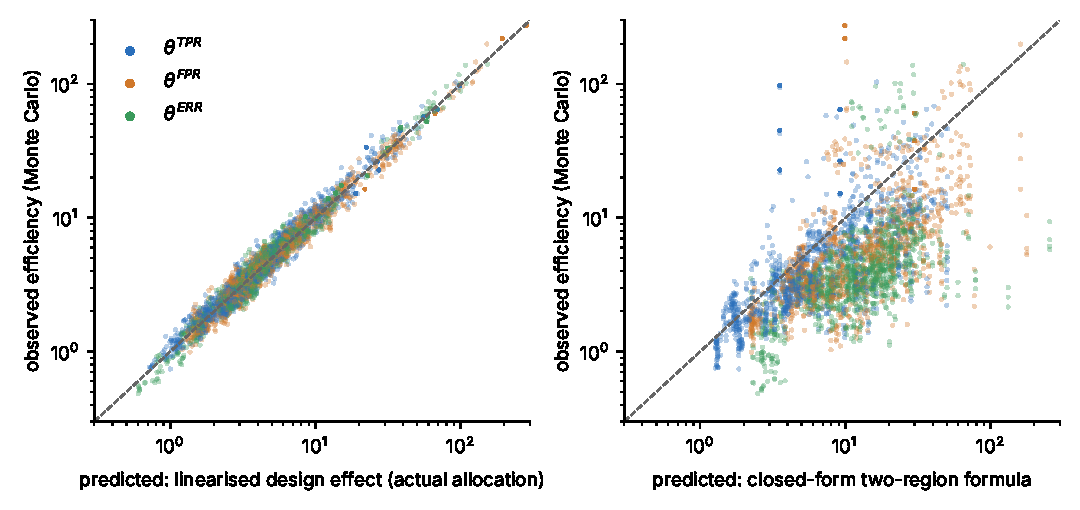
\includegraphics[width=\textwidth]{figures/fig_sim_real.pdf}
\caption{Real pools, all budgets: observed efficiency of PATTERN relative to SRS for each of the
3519 compared target--budget pairs against the linearised prediction LIN (left) and the closed-form
two-region formula FORM (right). Dashed: equality. Source: \texttt{results/theory\_check.json}.}
\label{fig:sim-real}
\end{figure}

\paragraph{The linearised design effect is accurate.} Over the 3519 pairs the ratio of observed to
predicted efficiency has median 0.998 and 10\%--90\% range 0.83--1.22; 77\% of the ratios are within
20\% and 99\% within a factor 1.5, and the correlation of the logarithms is 0.988
(Figure~\ref{fig:sim-real}, left). The spread is what Monte Carlo error alone produces: each MSE is
an average of 200 squared errors, with a relative standard error of about $\sqrt{2/200}=0.10$ for
approximately normal errors, so the ratio of two independent MSEs has a relative standard error of
about 0.14 and a 10\%--90\% range of roughly 0.84--1.20. The medians per pool and budget agree as
well: the ratio of the observed median efficiency to the median LIN prediction lies between 0.88 and
1.20 for the 34 pool--budget combinations, and for each type of estimand separately the median of
these ratios is 0.99 (TPR), 0.98 (FPR) and 1.00 (error). The agreement includes the cases with very
large gains: for Churn at $L=500$ the observed efficiency of 32.4 (predicted 32.2) arises because
the disagreement strata are fully enumerated, which only the finite-population corrections in LIN
capture. The lower correlations for Electricity, Phoneme and MAGIC reflect the narrow range of
efficiencies across targets in those pools (most lie between 2 and 4), not a larger error. We
conclude that, for the purpose of predicting efficiency, the linearised variance of
Section~\ref{sec:theory-asym} is adequate already at $L=250$.

\paragraph{The closed form overstates the gain on real pools.} FORM is a much poorer predictor: the
median ratio of observed efficiency to FORM is 0.47 (10\%--90\%: 0.17--1.17), and the rule of thumb
$1/\rho$ is more optimistic still (Table~\ref{tab:sim-real}). The reason is the one anticipated in
Section~\ref{sec:theory-deff}: with nine models the strata $(G,K)$ do not isolate the disagreements of
a particular pair. The share of the pool on which some model disagrees, $\rho_{\rm any}$, is between
0.18 and 0.73, while the median pairwise rate is between 0.001 and 0.33, and by
\eqref{eq:deff-sandwich} the attainable gain lies between $1/\rho_{\rm any}$ and $1/\rho$. OWN, which
uses the actual strata, is much closer (median ratio of observed to OWN 0.87): the remaining 13\% is
the price of serving all 108 estimands with one allocation, which Proposition~\ref{prop:allocation}(d)
makes explicit. Law school is a degenerate case for FORM, since the median pair disagrees on 0.1\% of
the pool and many targets have nearly zero variance; FORM and the observed efficiencies are
negatively correlated there. FORM is therefore useful as an explanation of where the gain comes from
and as an upper guide for a pair-specific design, but not as a numerical prediction for the
nine-model design; for prediction, LIN should be used, and it requires nothing beyond the pool and a
pilot or proxy estimate of the stratum variances.

\subsection{Synthetic pools with a controlled disagreement rate}\label{sec:sim-synth}

To test the closed form where its assumptions hold, and to vary $\rho$ over a wide range, we
generated pools of $N=200\,000$ with two groups ($\zeta_1=0.3$, $p_0=0.30$, $p_1=0.20$). A share
$\rho\in\{1,2,5,10,20,40\}\%$ of instances is placed in a disagreement region. Outside it, all models
predict the same label, equal to $Y$ with probability 0.85. Inside it, with two models, model 1 is
right with probability $q_g$ and model 2 predicts the opposite label; we use $q=(0.65,0.35)$
(moderate group-wise gaps) and $q=(0.95,0.05)$ (large gaps, one-sided disagreements). With five
models, each model is right independently with a model- and group-specific probability between 0.40
and 0.70, conditionally on not all models agreeing. Each model's probability is
$\mathrm{logit}^{-1}\{1.73(2\hat y-1)+\varepsilon\}$ with $\varepsilon\sim N(0,1)$, and the proxy is their
average, as in the real pools. The budget is $L=1000$ and $R=1000$, so the Monte Carlo relative
standard error of an efficiency is about 0.06. With two models, the pattern strata separate agreement
from disagreement exactly, and we also ran, for each target, its own Neyman allocation computed from
the true stratum variances, which is the design FORM describes.

\begin{table}[t]
\centering
\caption{Synthetic pools: observed (Obs), linearised (LIN) and closed-form (FORM) efficiency of
PATTERN relative to SRS for $\theta^{TPR}$ and $\theta^{ERR}$ (median over pairs for five models),
as a function of the disagreement rate $\rho$ ($N=200\,000$, $L=1000$, $R=1000$). Source:
\texttt{results/theory\_check.json}.}
\label{tab:sim-syn}
\setlength{\tabcolsep}{3pt}
\resizebox{\textwidth}{!}{%
\begin{tabular}{l rrr rrr @{\hskip 8pt} rrr rrr @{\hskip 8pt} rrr rrr}
\toprule
 & \multicolumn{6}{c}{Two models, moderate gaps} & \multicolumn{6}{c}{Two models, large gaps} & \multicolumn{6}{c}{Five models}\\
 \cmidrule(lr){2-7}\cmidrule(lr){8-13}\cmidrule(lr){14-19}
 & \multicolumn{3}{c}{$\theta^{TPR}$} & \multicolumn{3}{c}{$\theta^{ERR}$} & \multicolumn{3}{c}{$\theta^{TPR}$} & \multicolumn{3}{c}{$\theta^{ERR}$} & \multicolumn{3}{c}{$\theta^{TPR}$} & \multicolumn{3}{c}{$\theta^{ERR}$}\\
$\rho$ & Obs & LIN & FORM & Obs & LIN & FORM & Obs & LIN & FORM & Obs & LIN & FORM & Obs & LIN & FORM & Obs & LIN & FORM\\
\midrule
1\% & 190.3 & 216.0 & 102.2 & 174.1 & 181.1 & 115.5 & 56.2 & 55.8 & 46.2 & 665.4 & 608.0 & 517.0 & 172.9 & 198.3 & 170.7 & 158.1 & 162.9 & 203.2 \\
2\% & 54.3 & 57.4 & 43.7 & 56.7 & 58.2 & 55.7 & 22.2 & 26.0 & 23.4 & 251.5 & 240.7 & 261.2 & 44.9 & 64.2 & 82.9 & 49.8 & 55.3 & 99.7 \\
5\% & 14.9 & 18.6 & 16.6 & 23.2 & 20.2 & 22.1 & 10.0 & 9.7 & 9.5 & 88.1 & 83.1 & 103.7 & 17.4 & 21.0 & 32.9 & 19.5 & 19.6 & 40.1 \\
10\% & 7.2 & 8.9 & 8.4 & 8.6 & 9.6 & 10.9 & 4.4 & 5.1 & 5.1 & 45.6 & 42.5 & 53.5 & 9.2 & 11.0 & 17.5 & 8.9 & 9.4 & 20.1 \\
20\% & 4.4 & 4.7 & 4.6 & 5.0 & 4.8 & 5.5 & 2.4 & 2.8 & 2.8 & 16.7 & 20.3 & 25.6 & 4.9 & 5.4 & 9.0 & 4.7 & 4.6 & 10.0 \\
40\% & 2.3 & 2.5 & 2.5 & 2.4 & 2.4 & 2.7 & 1.7 & 1.6 & 1.8 & 9.5 & 10.1 & 12.4 & 2.5 & 2.8 & 4.7 & 2.3 & 2.3 & 5.0 \\
\bottomrule
\end{tabular}}
\end{table}

\begin{figure}[t]
\centering
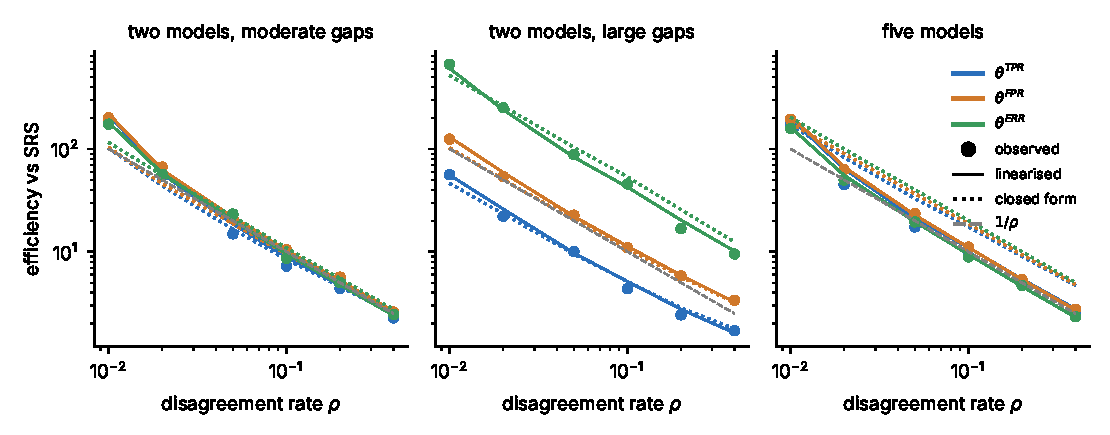
\includegraphics[width=\textwidth]{figures/fig_sim_rho.pdf}
\caption{Synthetic pools: efficiency of PATTERN relative to SRS against the disagreement rate
$\rho$ (share of the pool in the disagreement region), median over pairs for each type of estimand.
Points: Monte Carlo ($R=1000$); solid: linearised prediction LIN; dotted: closed form FORM;
grey dashed: $1/\rho$. Source: \texttt{results/theory\_check.json}.}
\label{fig:sim-rho}
\end{figure}

\paragraph{Efficiency scales as $1/\rho$.} In all three families the efficiency falls in proportion
to $1/\rho$ over a forty-fold range of $\rho$ (Figure~\ref{fig:sim-rho}). With two models and
moderate gaps, $\rho$ times the median observed efficiency is between 0.86 and 1.13 for
$\rho\ge2\%$, so the rule of thumb is accurate to about 15\%; at $\rho=1\%$ it is 1.9, because the
budget of 1000 labels is then about half the size of the disagreement region and the
finite-population correction roughly doubles the gain. LIN agrees with the observed efficiencies
throughout (median ratio per scenario between 0.88 and 1.04), with a tendency to be optimistic by a
few per cent that we attribute to the second-order terms neglected by the linearisation.

\paragraph{The closed form is accurate, and conservative, when its assumptions hold.} With two
models, the observed efficiency of the own-target Neyman design divided by FORM is between 0.90 and
1.25 for moderate gaps and $\rho\ge5\%$, and between 0.95 and 1.47 for large gaps; the LIN
predictions for the same designs give the same ratios, so the discrepancy is in the closed form and
not in the simulation. FORM is below the truth for two reasons stated in
Corollary~\ref{prop:deff}(a): it treats the agreement region as one stratum, whereas the pattern
design splits it by the common prediction ($K=0$ versus $K=M$, which have very different positive
rates), and it ignores the finite-population correction, which matters when the disagreement region
is small (at $\rho=1\%$ the ratio is 1.5 to 2.5). The large-gap family also shows the role of the
target size in Corollary~\ref{prop:deff}(c): the TPR gaps are large and the disagreements one-sided
($|a_g|=0.9$), and the gain for $\theta^{TPR}$ is only 0.45 to 0.7 times $1/\rho$, in line with
the factor $(\beta+\lambda)^{-2}$, which is about 0.4 for group 0 ($\pi_{\mathcal D}\approx
\pi_{\mathcal A}\approx0.3$) before the group factor $\Gamma$ is applied, while for the error difference, whose disagreements are nearly
deterministic within each group ($|\mu_g|=0.9$), the gain is several times $1/\rho$, as
\eqref{eq:deff-err} predicts.

\paragraph{With more models, the relevant rate is between $\rho_{\rm any}$ and the pairwise rate.} In
the five-model family the pairwise disagreement rate is about half of $\rho$, and FORM, which assumes
that each pair's disagreements are isolated, overstates the gain by a factor of about 1.9 (median
ratio of observed to FORM between 0.53 and 0.56 for $\rho\ge2\%$). The observed efficiency is instead
close to $1/\rho_{\rm any}$ ($\rho_{\rm any}$ times the median efficiency is between 0.94 and 1.03 for
$\rho\ge2\%$), the lower end of \eqref{eq:deff-sandwich}. This is expected: in this family the models
err independently inside the disagreement region, so a pair's disagreements are spread evenly over
the values of $K$. In the real pools, where models make correlated errors, the median OWN efficiency
lies inside the interval $[1/\rho_{\rm any},1/\rho]$ for every pool (Table~\ref{tab:sim-real}),
mostly in its lower half.

\subsection{Misspecified proxy}\label{sec:sim-proxy}

Proposition~\ref{prop:proxy} bounds the loss from a wrong proxy by the ratio \eqref{eq:proxy-loss}.
We took the five-model pool with $\rho=5\%$ and compared allocations computed from the default proxy,
from the true labels (oracle), from a constant proxy equal to the overall positive rate
(uninformative), from one minus the default proxy (inverted), and from an adversarial proxy that sets
$\pi_i=0.5$ where all models agree and $\pi_i=0.001$ where they do not, with proportional allocation
on the same strata as a reference.

\begin{table}[t]
\centering
\caption{Proxy misspecification (five models, $\rho=5\%$, $L=1000$, $R=1000$). Loss: weighted
variance $\sum_tw_tV_t$ relative to the oracle allocation, predicted by the linearisation (pred.) and
observed with MSEs (obs.). Eff: harmonic mean over the 30 estimands of the efficiency relative to
SRS, predicted and observed, and the smallest observed efficiency. Kant.: Kantorovich bound of
Proposition~\ref{prop:proxy}(c) evaluated with the actual allocation. Source:
\texttt{results/theory\_check.json}.}
\label{tab:sim-proxy}
\small
\begin{tabular}{lrrrrrr}
\toprule
Allocation & Loss pred. & Loss obs. & Eff pred. & Eff obs. & min Eff obs. & Kant.\\
\midrule
Default proxy & 1.00 & 1.01 & 22.0 & 20.5 & 15.4 & 1.24\\
Oracle & 1.00 & 1.00 & 21.9 & 20.6 & 17.1 & 1.07\\
Uninformative & 1.00 & 1.01 & 21.9 & 20.5 & 16.6 & 1.23\\
Inverted & 1.00 & 0.98 & 22.0 & 21.2 & 17.2 & 1.24\\
Adversarial & 1.00 & 0.98 & 21.9 & 21.0 & 15.9 & 1.21\\
Proportional & 8.48 & 7.85 & 2.6 & 2.6 & 2.1 & 56.21\\
\bottomrule
\end{tabular}
\end{table}

None of the four wrong proxies costs a measurable amount of efficiency (Table~\ref{tab:sim-proxy}):
the predicted loss is at most 0.2\%, the observed differences (between $-2.4\%$ and $+1.2\%$) are
within Monte Carlo error, and every one of the 30 estimands is estimated at least 15 times more
efficiently than under SRS. Proportional allocation on the same strata, by contrast, has eight times
the weighted variance. The explanation is Proposition~\ref{prop:influence}: the proxy enters the
anticipated stratum variances only through label rates, while the dominant feature, namely that the
comparison estimands receive almost no variance from the strata where all models agree, is fixed by
the predictions. With a constant or adversarial proxy the agreement strata are still anticipated to
have variance of order $\delta_g^2$, which is small, and the disagreement strata still have variance
of order one because $D_i$ varies within them; so all these allocations put almost the whole budget
into the disagreement strata and differ only in how it is divided among them. The Kantorovich bounds
(1.21--1.24) are valid but loose here. This robustness is specific to the structure of the problem
and should not be read as a general guarantee: Proposition~\ref{prop:proxy}(d) shows that a proxy
that misjudges a high-variance stratum can do arbitrarily badly in other stratified problems, and the
empirical comparison with the oracle allocation in Section~\ref{sec:empirical} is the relevant check
for real data.

\subsection{Summary}

The linearised design effect predicts the efficiency of the implemented design to within Monte
Carlo error on all 11 real pools and in the synthetic families (per-target median ratio 1.00,
10\%--90\% range 0.83--1.22 on the real pools). The closed form of Corollary~\ref{prop:deff} is
accurate and conservative when the strata separate a pair's agreements from its disagreements (the
own-target efficiency is 0.90 to 1.47 times the formula for $\rho\ge5\%$), and it captures the $1/\rho$ scaling and the effect of the
target size. With nine models it overstates the gain on real pools by a median factor of about two,
because the counts $K$ locate any disagreement but not that of a specific pair; the bounds
$1/\rho_{\rm any}\le\mathrm{Eff}\le1/\rho$ of \eqref{eq:deff-sandwich} describe this gap. The gain vanishes
only as the disagreement rate approaches one, as in EEG ($\rho_{\rm any}=0.73$, efficiency 1.6--1.9).

\section{Baseline designs and detailed results}\label{si:baselines}

This section gives the full definitions of the baselines compared in Section~\Mref{sec:baselines}, the per-setting results and the detailed coverage discussion.

\paragraph{Common ground.} To make the comparison about the choice of labels and estimators and nothing else, every method estimates the same vector of totals $T$ (Section~\Mref{sec:setting}), plugs it into the same map $\hat\theta=f(\hat T)$ for all $3\binom{M}{2}=108$ comparison estimands $\theta^{\mathrm{TPR}}_{mj},\theta^{\mathrm{FPR}}_{mj},\theta^{\mathrm{ERR}}_{mj}$, and reports 95\% Wald intervals from a linearisation variance. Every method that uses a proxy uses the same $\pi_i=M^{-1}\sum_m\hat p_{mi}$, and every allocation over several estimands uses the same weights $w_k=1/S_k^2$ as (\Mref{eq:alloc}). The budget is counted in distinct labelled instances. Pool labels are used only to answer label queries, to compute the truth and, for reporting, to pick the three most accurate models. Estimands whose numerator is identically zero in the pool (the two models never disagree on the relevant instances) are estimated exactly by every design and are left out of all summaries. This removes 51 of the 108 estimands in the law-school setting, including all those among its three most accurate models, and none elsewhere.

\subsection{Baseline definitions}


\paragraph{B1: importance sampling for active comparison.} \citet{sawade2012active} compare the risks of two fixed models by drawing $n$ instances with replacement from an instrumental distribution $q$ and estimating each risk by the self-normalised weighted mean $\sum_k \ell_k/q_k\big/\sum_k 1/q_k$ (with $p(x)=1/N$ on a pool). Their Theorem~1 shows that the asymptotic variance of the estimated risk difference is minimised by $q^*(x)\propto p(x)\{\mathbb E[(\ell_1-\ell_2-\Delta)^2\mid x]\}^{1/2}$. They replace $p(y\mid x)$ by an equal mixture of the models' predictive distributions, and for $k$ models they use the equal mixture of the pairwise-optimal distributions. We keep all of this and change only the quantity being compared. With replacement draws $i_1,\dots,i_n\sim q$, our totals are the Hájek (self-normalised) estimators
\begin{align*}
\hat T^{\mathrm{IS}}&=N\,\frac{\sum_{k=1}^n t_{i_k}(Y_{i_k})/q_{i_k}}{\sum_{k=1}^n 1/q_{i_k}},\\
\hat\theta-\theta&\approx\frac1n\sum_{k=1}^n \frac{a_{i_k}}{q_{i_k}},\\
a_i&=\nabla f(T)^{\top}\{t_i(Y_i)-T/N\}.
\end{align*}
For $\theta^{\mathrm{ERR}}_{mj}$, $a_i=\{|\hat y_{mi}-Y_i|-|\hat y_{ji}-Y_i|-\theta^{\mathrm{ERR}}_{mj}\}/N$, which is exactly Sawade et al.'s centred loss difference. For $\theta^{\mathrm{TPR}}_{mj}$, the self-normalisation is automatic because $f$ is a ratio, and $a_i=\sum_g s_g\,\mathbf 1\{G_i=g\}\,Y_i\{(\hat y_{mi}-\hat y_{ji})-(\mathrm{TPR}_{mg}-\mathrm{TPR}_{jg})\}/P_g$. The asymptotic variance is $n^{-1}\sum_i\mathbb E[a_i^2]/q_i$ \citep{hansen1943}, so the single-estimand optimum is $q_i\propto\{\mathbb E_\pi a_i^2\}^{1/2}$, with the expectation taken under $Y_i\sim\mathrm{Bernoulli}(\pi_i)$ and $a$ evaluated at the proxy totals. This is our adaptation to TPR and FPR gaps. For a pair $(m,j)$ we combine its three estimands as $q^{(mj)}_i\propto\{\sum_{k\in(m,j)}w_k\mathbb E_\pi a_{ik}^2\}^{1/2}$. The design distribution is the equal mixture over the 36 pairs, as in Sawade et al., mixed with the uniform distribution with weight $0.05$ so that every $q_i$ is bounded away from zero. Draws continue until $L$ distinct instances are labelled; repeated draws reuse the label. The median number of draws was $1.12L$ (range $1.02L$--$1.48L$), so B1 effectively gets more than $L$ draws for $L$ labels. The variance is estimated by $n^{-1}$ times the sample variance of $\hat a_{i_k}/q_{i_k}$.

\paragraph{B2: proxy-score stratification.} The classic approach to estimating a classifier's metrics with few labels stratifies on the classifier's score and allocates optimally \citep{bennett2010online,kumar2018classifier}. We form strata as group $\times$ within-group quantile bins of $\pi_i$ (10 bins, Score-10; and 5 bins, Score-5), merge strata smaller than 50 as for PATTERN, and use the same estimator (\Mref{eq:HT}), variance (\Mref{eq:var}) and proxy-Neyman allocation (\Mref{eq:alloc}). B2 therefore differs from PATTERN only in the strata. It uses the proxy strongly but ignores which models disagree.

\paragraph{B3: disagreement-focused two-phase design.} Labelling only where models disagree is the ``active $\neq$'' baseline of \citet{sawade2012active} and the discordant-pair approach of \citet{musgrove2023discordant} and of the screening-test literature \citep{pepe2001comparing}. On its own it identifies only ratios, because the denominators $P_g,Q_g$ need labels in the agreement set. Let $D=\{i:0<K_i<M\}$ and $A=U\setminus D$. Phase 1 draws a simple random sample $s_0$ of size $n_0$ from $U$. Phase 2 draws a simple random sample of $L-n_0$ from $D\setminus s_0$. Conditionally on $n_A=|s_0\cap A|$, the labelled units in $A$ are a simple random sample from $A$. Conditionally on $|s_0\cap D|$, the union of $s_0\cap D$ and the phase-2 sample is a simple random sample of size $n_D=|s_0\cap D|+L-n_0$ from $D$. The combined estimator is therefore the two-stratum estimator $\hat T=N_A\bar t_A+N_D\bar t_D$ with variance (\Mref{eq:var}) at the realised $(n_A,n_D)$, which is conditionally design-unbiased. We take $n_0=L/4$ (Dis-25) and $n_0=L/2$ (Dis-50).

\paragraph{B4: prediction-powered inference.} PPI \citep{angelopoulos2023ppi} corrects the predictions on the whole pool with the labelled residuals. With the prediction of $t_i$ taken as its proxy mean $\tilde t_i=\pi_iu_i+(1-\pi_i)v_i$, the PPI estimator of a total under SRS is the difference estimator
\[
\hat T^{\mathrm{PPI}}_\lambda=\lambda\sum_{i\in U}\tilde t_i+\frac Nn\sum_{i\in s}\{t_i(Y_i)-\lambda\tilde t_i\},
\]
with $\lambda=1$ (PPI). PPI++ \citep{angelopoulos2026ppipp} tunes $\lambda$ for each estimand. In our finite-pool setting the predictions are known for every unit, so the $(1+n/N)$ factor of PPI++ drops out and the variance-minimising value is the regression coefficient of $\nabla f^\top t_i$ on $\nabla f^\top\tilde t_i$ in the sample. We clip it to $[0,1]$. StratPPI \citep{fisch2024stratppi} applies PPI++ within strata with a stratum-specific $\lambda_{hk}$ and allocates the budget by a Neyman rule on the residual standard deviation, estimated from the predictor's own confidence scores. We use the B2 strata (group $\times$ 10 proxy bins), per-stratum and per-estimand $\lambda_{hk}$ clipped to $[0,1]$, and the allocation $n_h\propto N_h\{\sum_k w_k\,\overline{\pi(1-\pi)(A_{k}-B_{k})^2}_h\}^{1/2}$. Here $\pi_i(1-\pi_i)(A_{ik}-B_{ik})^2$ is the proxy variance of the residual $z_{ik}-\mathbb E_\pi z_{ik}$, so this allocation is Fisch et al.'s confidence-based rule for our estimands. In all three versions the variance is the stratified formula (\Mref{eq:var}) applied to the residuals $z_{ik}-\lambda\,\nabla f^\top\tilde t_i$.

\paragraph{B5: PATTERN with a model-assisted estimator (the proposed method).} The PPI correction is a difference or GREG-type estimator \citep[Chapter~6]{sarndal1992} and can be applied to the PATTERN sample without changing the design. PATTERN-DIF uses the stratified difference estimator with $\lambda=1$. PATTERN-PPI tunes $\lambda_{hk}$ per stratum as in StratPPI. B5 is the proposed method (PATTERN-DIF, $\lambda=1$) and a tuned-weight variant (PATTERN-PPI), and is reported in the last block of the results.

\paragraph{Not run.} Active testing with LURE \citep{kossen2021active}, adaptive variance-minimising selection \citep{hara2024}, and active inference \citep{zrnic2024active,li2025robust} select labels sequentially and target one estimand of one model. Their fixed-budget, one-shot analogue for our vector of estimands is B1, which uses the same proxy-optimal inclusion principle. Model-based estimators that need a fitted joint model of labels and scores (for example SSME) are outside the design-based comparison made here.

\subsection{Detailed results}

\begin{figure}[t]\centering
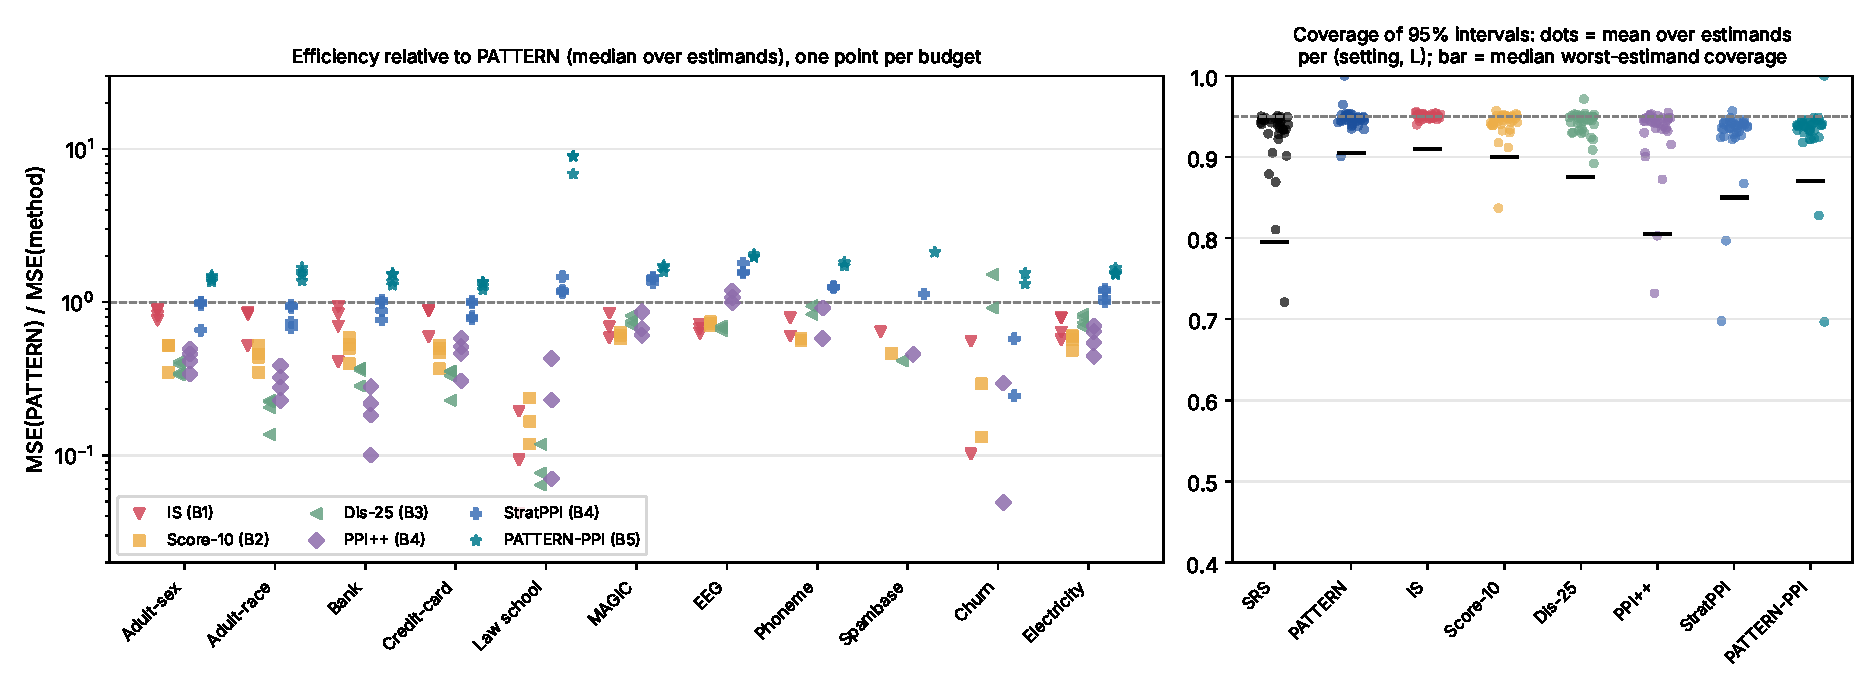
\includegraphics[width=\textwidth]{figures/base_efficiency.pdf}
\caption{Left: MSE(PATTERN)/MSE(method) by setting, one point per budget, median over comparison estimands (values above 1 mean that the method beats PATTERN; the axis is clipped to $[0.02,30]$ and law school at $L=2000$ is not shown in range because PATTERN labels the whole disagreement set there). Right: mean coverage of the nominal 95\% interval over estimands for each (setting, $L$), with the median over cells of the worst-estimand coverage as a bar. Source: \texttt{results/label\_baselines.json}.}\label{fig:base-efficiency}
\end{figure}

\begin{table}[t]\centering\small
\caption{Efficiency relative to PATTERN, MSE(PATTERN)/MSE(method), median over estimands, by setting at $L=500$ ($L=250$ for Spambase, whose pool is too small for $L=500$). Values above 1 mean that the method beats PATTERN. Second column: efficiency of PATTERN relative to SRS. Last two columns: mean coverage of the 95\% intervals of StratPPI and of PATTERN-PPI. Source: \texttt{results/label\_baselines.json}.}\label{tab:base-setting}
\setlength{\tabcolsep}{3.5pt}
\begin{tabular}{l rrrrrrrrrrr}\toprule
 & PAT. & \multicolumn{6}{c}{Baselines (B1--B4) vs PATTERN} & \multicolumn{2}{c}{B5 vs PATTERN} & \multicolumn{2}{c}{Coverage} \\
\cmidrule(lr){3-8}\cmidrule(lr){9-10}\cmidrule(lr){11-12}
Setting & vs SRS & IS & Score-10 & Dis-25 & Dis-50 & PPI++ & StratPPI & PATTERN-DIF & PATTERN-PPI & StratPPI & PAT-PPI \\ \midrule
Adult-sex & 4.19 & 0.89 & 0.52 & 0.39 & 0.37 & 0.46 & 0.97 & 1.45 & 1.49 & 0.935 & 0.939 \\
Adult-race & 7.27 & 0.86 & 0.46 & 0.23 & 0.22 & 0.32 & 0.93 & 1.44 & 1.58 & 0.939 & 0.939 \\
Bank & 8.26 & 0.84 & 0.50 & 0.36 & 0.38 & 0.22 & \textbf{1.03} & 1.47 & 1.52 & 0.941 & 0.933 \\
Credit-card & 3.71 & 0.89 & 0.52 & 0.36 & 0.35 & 0.51 & \textbf{1.01} & 1.28 & 1.35 & 0.937 & 0.933 \\
Law school & 39.0 & 0.09 & 0.24 & 0.08 & 0.08 & 0.23 & \textbf{1.47} & 11.1 & 8.97 & 0.797 & 0.828 \\
MAGIC & 2.93 & 0.69 & 0.63 & 0.75 & 0.63 & 0.67 & \textbf{1.43} & 1.70 & 1.73 & 0.942 & 0.943 \\
EEG & 1.70 & 0.67 & 0.73 & 0.70 & 0.66 & \textbf{1.19} & \textbf{1.57} & 1.98 & 2.05 & 0.926 & 0.939 \\
Phoneme & 3.53 & 0.60 & 0.58 & 0.83 & 0.67 & 0.58 & \textbf{1.26} & 1.71 & 1.72 & 0.946 & 0.941 \\
Spambase$^{\ast}$ & 5.77 & 0.64 & 0.46 & 0.42 & 0.37 & 0.46 & \textbf{1.13} & 2.14 & 2.12 & 0.925 & 0.933 \\
Churn & 34.6 & 0.10 & 0.13 & \textbf{1.52} & 0.28 & 0.05 & 0.24 & 1.28 & 1.32 & 0.930 & 0.932 \\
Electricity & 2.86 & 0.79 & 0.59 & 0.80 & 0.73 & 0.64 & \textbf{1.21} & 1.49 & 1.53 & 0.942 & 0.933 \\
\bottomrule\end{tabular}\end{table}


\paragraph{Where a baseline beats PATTERN.} Table~\ref{tab:base-setting} and Figure~\ref{fig:base-efficiency} show where the ranking changes. First, StratPPI beats PATTERN at $L=500$ in seven of the ten settings of the table (ratios 1.01--1.57 in Bank, Credit-card, Law school, MAGIC, EEG, Phoneme and Electricity, and 1.13 in Spambase at $L=250$), and is below it in Adult-sex (0.97), Adult-race (0.93) and Churn (0.24). Over all cells its ratio exceeds 1 in 19 of 35 (median 1.12 at $L=500$). The margin is small in most settings, and it is not a failure of the stratification: StratPPI uses the same sample size but a model-assisted estimator, and B5 shows that the same correction applied to the PATTERN sample improves PATTERN itself by a median factor of 1.3--1.7. Second, Dis-25 beats PATTERN on Churn at $L=500$ (ratio 1.52); there the pool has a 19\% disagreement set, PATTERN strata are mostly small, and Dis-25 labels most of its sample inside the disagreement set. Its intervals are not reliable in that cell: mean coverage 0.93 but worst-estimand coverage 0.66, so the apparent gain should be read with caution. Third, PPI++ beats PATTERN on EEG (ratio 1.19 at $L=500$), the setting with the largest disagreement set (73\%), where agreement cells hold little and the proxy is informative. Importance sampling never beats PATTERN in the all-estimand median (ratio below 1 in all 35 cells), but on the pairs among the three most accurate models it is competitive: its median efficiency against SRS on those pairs is 4.2, 4.1, 4.2 and 6.3 at $L=250,\dots,2000$, against 3.4, 3.6, 4.0 and 6.8 for PATTERN, and it beats PATTERN on those pairs in 10 of 35 cells (Adult-sex: 1.49 at $L=250$ and 1.10 at $L=500$, while its all-estimand ratio there is 0.89). Where the question is only about the best few models, importance sampling is a serious alternative.

\paragraph{Where PATTERN wins clearly.} In the two settings with the lowest disagreement rate, Law school and Churn, PATTERN is 6--84 times more efficient than SRS at $L\le1000$ and PATTERN labels essentially every disagreement instance at $L=2000$ in Law school (all non-degenerate estimands then have error close to zero, ratio above $10^{20}$, so these cells are shown as $>$100 and excluded from the figure range). IS, Dis-50, score strata and PPI++ reach only 0.04--0.7 of PATTERN's efficiency there (Dis-25 on Churn is the exception discussed above), because none of them isolates the agreement region exactly: PATTERN gives it a stratum of its own that can be labelled sparsely, while the other designs either draw it at random or leave the disagreement set under-sampled.

\paragraph{Coverage and failures.} Over all 35 cells the mean 95\% coverage is 0.925 (SRS), 0.947 (PATTERN), 0.950 (IS), 0.941 (Score-10), 0.942 (Dis-25), 0.929 (PPI++), 0.924 (StratPPI), 0.946 (PATTERN-DIF) and 0.929 (PATTERN-PPI). The shortfalls concentrate in the smallest cells. The lowest worst-estimand coverages over all cells are 0.14 for StratPPI (Churn, $L=250$), 0.16 for SRS and for PPI++, 0.17 for Score-10, 0.20 for PATTERN-PPI, 0.45 for Dis-25 and 0.52 for PATTERN (Churn, $L=250$). The tuned estimators (PPI++, StratPPI, PATTERN-PPI) undercover when per-stratum tuning parameters are estimated from a few labels, notably in Law school where PATTERN-PPI covers 0.70 at $L=250$ and StratPPI 0.70--0.87 below $L=2000$. PATTERN-DIF, which fixes $\lambda=1$, keeps the coverage of PATTERN (0.946). Undefined estimates (a group with no sampled positive) occurred in at most 1\% of replications for any method (Dis-25, Adult-race, $L=250$: 1\%; SRS 0.5\%; PATTERN and the others none). Runtimes per replicate (design computation excluded) are 8--11 ms on average for the stratified and importance-sampling designs and 34--51 ms for the PPI-type estimators (Table~\Mref{tab:base-budget}, last column), which tune per estimand and stratum. Design computation is at most 0.6 s per cell for every method.

\paragraph{The model-assisted extension.} PATTERN-DIF and PATTERN-PPI (bottom block of Table~\Mref{tab:base-budget}) improve on PATTERN in every cell except Law school at $L=2000$, where PATTERN is already exact, by a median factor of 1.3--1.6 (by budget) and up to 11 in Law school at $L\le500$; they are the best methods in this study, with efficiency against SRS of 6.6, 6.2, 6.6 and 15.5 for PATTERN-DIF. The estimated-$\lambda$ version adds little over $\lambda=1$ (PATTERN-PPI is within 3\% of PATTERN-DIF in the median) and costs coverage, so we recommend the fixed-$\lambda$ version if the extension is used. Because the extension changes the estimator rather than the design, its variance expressions are those of the difference estimator under stratified sampling \citep{sarndal1992}. For $\lambda=1$ (PATTERN-DIF) unbiasedness, the variance formula and the asymptotic coverage are covered by Proposition~\Mref{prop:validity} with the proxy mean as $\psi$; for the tuned weights of PATTERN-PPI only the asymptotic statement of Proposition~\ref{prop:dif-lambda} holds, and the finite-sample undercoverage reported above is not covered by the theory.

\paragraph{Limitations (detail).} The comparison is restricted to fixed-budget, one-shot designs on cached pools of nine models with logistic-type probabilities; the proxy is the same for every method, so a better proxy for any of them (for example a calibrated or learned one) could change the ranking, especially for StratPPI and PATTERN-PPI which rely on it directly. The importance-sampling baseline draws with replacement and so spends more than $L$ draws for $L$ labels; counting draws instead of labels would lower its efficiency. $R=200$ replications give Monte Carlo errors of about 10\% on a single mean squared error, so differences between 0.9 and 1.1 in Table~\ref{tab:base-setting} should not be read as ranking. Medians over estimands hide estimand-level differences: on the three types, PATTERN's median efficiency against SRS is 6.2 (TPR), 4.8 (FPR) and 3.8 (ERR), against 3.0, 3.5 and 3.0 for IS and 5.3, 5.2 and 2.3 for StratPPI.

\section{Ablation studies: details}\label{si:ablations}

This section gives the full protocol and discussion of the ablation studies summarised in Section~\Mref{sec:ablations}. Tables for the stratifier (A1) and for small-sample inference (A4) are in the main text (Tables~\Mref{tab:abl-design} and~\Mref{tab:abl-inference}); the others are below.

This section varies one ingredient of PATTERN-DIF at a time and asks two questions: does the estimator remain valid, and how much efficiency is gained or lost relative to the default? The default is the method of the main study: strata $(G_i,K_i)$ with strata smaller than 50 merged within group, weighted generalised Neyman allocation \citep{neyman1934} computed with the ensemble-mean proxy $\pi_i$, a floor of 10 labels per stratum, the stratified difference estimator with $\lambda=1$ and the same proxy, and 95\% Wald intervals from the linearisation variance. The estimator that uses the proxy only to allocate labels, the plain (Horvitz--Thompson) estimator, is called HT or $\lambda=0$. Because the proxy now enters the estimator as well as the allocation, the proxy ablations report the two roles separately, and every ablation reports the difference estimator and, where it is informative, HT on the same samples. All results come from \texttt{experiments/label\_ablations\_dif.py} (helpers in \texttt{tcs/labeling\_variants\_dif.py}) and are stored in \texttt{results/label\_ablations\_dif.json}. An earlier version of this study, in which the plain estimator was the default, is not reported; where its conclusions differ they are noted below.

\paragraph{Protocol.} We use the eleven cached pools and budgets $L\in\{250,500,1000\}$ with $L\le N/4$ (29 setting--budget cells) and $R=150$ replications per cell and design. The first seven designs (SRS, GROUP, PATTERN and four alternative stratifiers) draw the same samples as an earlier version of this ablation study that used the plain estimator throughout (\texttt{results/label\_ablations.json} in the repository); we call it the earlier plug-in study and refer to its numbers where they are compared, so that differences between the two studies are due to the estimator alone. There are 108 comparison targets for the 36 pairs of nine models; targets whose numerator vanishes identically in the pool are exact for every design and are excluded (only Law school, where 57 remain). Efficiency is the per-target ratio $\mathrm{MSE}_{\mathrm{SRS}}/\mathrm{MSE}_{\mathrm{design}}$ with SRS and the plain estimator as reference, clipped to $[10^{-4},10^{4}]$, summarised by the median over targets and then over cells. ``Rel.'' is the median over cells of $\mathrm{MSE}_{\mathrm{PATTERN\text{-}DIF}}/\mathrm{MSE}_{\mathrm{variant}}$ (above one favours the variant) and ``Win'' the share of cells with Rel.\ above one. Coverage is the mean over targets and the worst target. With $R=150$ the Monte Carlo standard error of one coverage is about 0.018 and the minimum over 108 targets that all cover exactly 95\% has mean 0.90, so worst-target coverage near 0.90 is consistent with nominal behaviour and values well below 0.88 are not. A design with more strata than the budget can feed at 10 labels each uses the floor $\max(2,\lfloor 0.8L/H\rfloor)$. Undefined estimates occurred in at most 0.7\% of replications.

\subsection{Stratifier (A1)}

Table~\Mref{tab:abl-design} varies the stratifier; per-cell values are in Table~\ref{tab:abl-app-eff-design} of Section~\ref{si:ablation-tables}. On the same samples the difference estimator is more efficient than HT in all 29 cells (median ratio 1.67, range 1.36 to 14.5 in Law school), and its efficiency against SRS is 6.3 at every budget, compared with 3.6 to 4.3 for HT. The two gains are not additive: SRS with the difference estimator (SRS-DIF, i.e.\ PPI of \citealt{angelopoulos2023ppi} with the ensemble proxy) gains a factor 1.9, the PATTERN design with HT a factor 4.0 over all budgets, and the product of these medians (7.5) exceeds the combined gain.

The stratifier conclusions of the earlier study carry over. Group $\times$ agree/disagree keeps 74\% of the default's precision (earlier 71\%) and the joint pattern of the three models agreeing most with the ensemble keeps 38\% (earlier 37\%): the count $K_i$ is what matters, and three models cannot isolate the disagreement among 36 pairs. Splitting each $(G,K)$ cell at the median of $\pi_i$ is a tie (Rel.\ 1.01, better in 15 of 29 cells; by budget 0.99, 0.97, 1.04), as are tertile bins (0.99), whose extra strata eat the budget through the floor (3 to 9 labels where it binds). We keep $K_i$. The allocation tailored to the variance of the difference estimator (\texttt{'resid'} in \texttt{tcs.labeling\_dif}) is not better than the plain allocation (Rel.\ 0.96, better in 13 cells). The references that drop an ingredient lose clearly: GROUP-DIF and SRS-DIF keep 28\%, proportional allocation 57\% (earlier 52\%) and the gap-targeted allocation of A5 74\% (earlier 74\%). Coverage hardly depends on the stratifier (mean 0.938 to 0.946).

\subsection{Proxy and the role of $\lambda$ (A2)}

The proxy now has two jobs, and the ablation separates them (Table~\ref{tab:abl-proxy}; Figure~\ref{fig:abl-proxy} in Section~\ref{si:ablation-tables} shows the per-cell spread). The first block uses a proxy $\tilde\pi$ only to allocate labels and analyses the sample with HT. The second uses the same $\tilde\pi$ in the allocation and in the estimator, through the proxy mean $\psi_i=\tilde\pi_iu_i+(1-\tilde\pi_i)v_i$. The third allocates with $\tilde\pi$ but keeps the ensemble proxy in the estimator.

\emph{Allocation only.} As in the earlier study, the allocation is insensitive to the proxy. With HT, every proxy gives a median efficiency of 3.95 to 4.05 against 3.97 for the ensemble mean, including the reversed proxy $1-\pi$, the shuffled proxy and the constant 0.5; allocation by the true labels gives 3.71. With the ensemble proxy kept in the estimator, the alternative allocations keep 99\% to 101\% of the default's precision (Rel.\ in Table~\ref{tab:abl-proxy}, last block), with per-cell ratios between 0.86 and 1.4 except in Churn at $L=500$, where the constant, naive Bayes and shuffled proxies label the small disagreement strata exhaustively and gain factors of 19, 13 and 6 (1.8 for the logistic proxy). The reason is the same as before: the influence values vary within a stratum mainly through the differences $\hat y_{mi}-\hat y_{ji}$, known without labels. What matters in the allocation is that it is Neyman-type rather than proportional (Rel.\ 0.57).

\emph{Proxy in the estimator.} Here the proxy matters. Replacing the ensemble mean by a single model costs 13\% (logistic regression) or 42\% (naive Bayes, whose probabilities are extreme); the constant 0.5 costs 16\%, a shuffled proxy 47\%, a noisy proxy 39\% and the reversed proxy 34\% (Table~\ref{tab:abl-proxy}, middle block). The difference estimator remains unbiased and its coverage is unaffected (mean 0.940 to 0.949), as the theory predicts, so a poor proxy costs efficiency only. A corrupted proxy also removes the gain over HT on the same sample: the median ratio of DIF to HT is 0.96 for the shuffled and noisy proxies and 1.00 for naive Bayes, against 1.67 for the ensemble, and DIF is less efficient than HT in 19, 18 and 15 of 29 cells for these three. The constant keeps most of the gain (ratio 1.40) because $\psi_i$ still carries the known structure of $u_i,v_i$.

\begin{table}[t]
\centering\footnotesize
\setlength{\tabcolsep}{4pt}
\caption{Proxy ablation (A2). Eff.: median over all 29 cells of the median-over-targets efficiency vs SRS (plain estimator); Rel.: relative to PATTERN-DIF with the ensemble proxy (as in Table~\Mref{tab:abl-design}); worst: mean over cells of the worst-target coverage; mean: mean coverage. In the first block the proxy enters only the allocation and the sample is analysed with HT; in the second it enters allocation and estimator; in the third only the allocation, the estimator keeps the ensemble proxy. The true-label proxy is not defined as an estimator proxy (the estimator would be exact).}
\label{tab:abl-proxy}
\resizebox{\textwidth}{!}{\begin{tabular}{lcccccccccc}
\toprule
 & \multicolumn{3}{c}{Proxy in allocation only (HT)} & \multicolumn{4}{c}{Proxy in both (DIF)} & \multicolumn{2}{c}{DIF, ensemble in estimator} \\
\cmidrule(lr){2-4}\cmidrule(lr){5-8}\cmidrule(lr){9-10}
Proxy & Eff. & Rel. & worst & Eff. & Rel. & mean & worst & Eff. & Rel. \\
\midrule
Ensemble mean $\pi$ (default) & 3.97 & 0.65 & 0.858 & 6.27 & 1.00 & 0.945 & 0.877 & 6.27 & 1.00 \\
Single model (logistic) & 3.96 & 0.64 & 0.861 & 5.56 & 0.87 & 0.943 & 0.886 & 6.01 & 0.99 \\
Single model (naive Bayes) & 4.05 & 0.63 & 0.858 & 3.88 & 0.58 & 0.942 & 0.873 & 5.99 & 1.01 \\
Constant 0.5 & 3.97 & 0.62 & 0.850 & 5.71 & 0.84 & 0.940 & 0.858 & 6.01 & 0.99 \\
$\pi$ shuffled within group & 3.95 & 0.62 & 0.854 & 3.70 & 0.53 & 0.949 & 0.889 & 6.12 & 0.99 \\
$\pi$ with logit noise (sd 2) & 4.05 & 0.64 & 0.854 & 3.46 & 0.61 & 0.949 & 0.877 & 5.91 & 0.99 \\
Reversed, $1-\pi$ & 3.99 & 0.63 & 0.859 & 4.38 & 0.66 & 0.941 & 0.872 & 6.23 & 0.99 \\
True labels (allocation only) & 3.71 & 0.64 & 0.865 & -- & -- & -- & -- & 6.01 & 1.00 \\
\addlinespace
Proportional allocation (no proxy in allocation) & 2.05 & 0.38 & 0.819 & 3.75 & 0.57 & 0.943 & 0.877 & -- & -- \\
\bottomrule
\end{tabular}
}
\end{table}

\emph{The weight $\lambda$.} Table~\ref{tab:abl-lambda} (Section~\ref{si:ablation-tables}) compares $\lambda=0$ (HT), $\lambda=1$ (default) and a $\lambda$ tuned per stratum and target on the labelled units and clipped to $[0,1]$ \citep[as in PPI++ and StratPPI;][]{angelopoulos2026ppipp,fisch2024stratppi}. With the ensemble proxy the tuned version is slightly more efficient than $\lambda=1$ (median Rel.\ 1.016, better in 24 of 29 cells; 1.026 at $L=250$) but it undercovers: mean 0.923, worst target 0.799 on average and 0.227 in Law school at $L=250$, against 0.945, 0.877 and 0.633 for $\lambda=1$. The tuned weights are estimated from a few labels per stratum and the variance estimate ignores that. With a degraded proxy the tuned version is the more efficient of the three (shuffled 5.2, noisy 5.1, reversed 5.4, against 3.7, 3.5 and 4.4 at $\lambda=1$ and about 4.0 for HT), because it shrinks the correction, but again at coverage 0.92 to 0.93. Neither alternative is better than $\lambda=1$ with the ensemble proxy in both efficiency and validity, so we keep $\lambda=1$. Tuning is worth considering only when the proxy is known to be poor and some undercoverage is acceptable.

\subsection{Number of compared models (A3)}

For $M\in\{2,3,5\}$ we drew three random subsets of the nine models per size (the subsets of the earlier study), rebuilt strata, proxy and estimands from the subset only, and compared PATTERN-DIF and PATTERN-HT with SRS on the $3\binom{M}{2}$ targets. Subsets in which all models agree on every instance are dropped. Table~\ref{tab:abl-models} and Figure~\ref{fig:abl-models} show, as before, that the gain is governed by the share of the pool on which the compared models disagree rather than by $M$: the Spearman correlation between log efficiency and the disagreement share across the 284 configurations is $-0.72$, $-0.74$ and $-0.76$ at $L=250$, 500 and 1000 (HT: $-0.81$, $-0.78$, $-0.79$), and within settings at $L=250$ it is negative in all eleven (median $-0.43$). At $L=250$ the median efficiency of PATTERN-DIF is 17.2 when the compared models disagree on less than 10\% of the pool, 12.5 for 10 to 20\%, 4.8 for 20 to 40\% and 3.8 above 40\%. What the difference estimator changes is the size of the gain over HT, which grows with $M$ from 1.15 at $M=2$ to 1.67 at $M=9$. The log ratio of DIF to HT is positively correlated with the disagreement share (0.09, 0.19, 0.34 by budget). The correction therefore helps most where the design alone helps least, but it does not remove the dependence on disagreement. Coverage is not affected by $M$ (mean 0.945 to 0.950); the worst-target figures cannot be compared across rows, because the number of targets grows from 3 to 108.

\begin{table}[t]
\centering\small
\caption{Number of compared models (A3). Configs: (setting, budget, subset) combinations; Disagr.: median share of the pool on which not all $M$ models agree. Efficiency: median over configurations of the median-over-targets $\mathrm{MSE}_{\mathrm{SRS}}/\mathrm{MSE}$. DIF/HT: median ratio of the two efficiencies on the same sample. Coverage: PATTERN-DIF, Wald.}
\label{tab:abl-models}
\resizebox{\textwidth}{!}{\begin{tabular}{rccccccccc}
\toprule
 & & & \multicolumn{3}{c}{PATTERN-DIF vs SRS} & \multicolumn{1}{c}{PATTERN-HT vs SRS} & & \multicolumn{2}{c}{Coverage (DIF)} \\
\cmidrule(lr){4-6}\cmidrule(lr){9-10}
$M$ & Configs & Disagr. & $L=250$ & 500 & 1000 & all $L$ & DIF/HT & mean & worst \\
\midrule
2 & 87 & 0.133 & 9.48 & 12.58 & 9.28 & 8.37 & 1.15 & 0.950 & 0.933 \\
3 & 84 & 0.193 & 8.29 & 10.70 & 8.57 & 6.44 & 1.27 & 0.949 & 0.919 \\
5 & 84 & 0.294 & 7.62 & 6.64 & 7.08 & 4.78 & 1.52 & 0.946 & 0.904 \\
9 & 29 & 0.396 & 6.27 & 6.18 & 6.37 & 3.97 & 1.67 & 0.945 & 0.877 \\
\bottomrule
\end{tabular}
}
\end{table}

\begin{figure}[t]
\centering
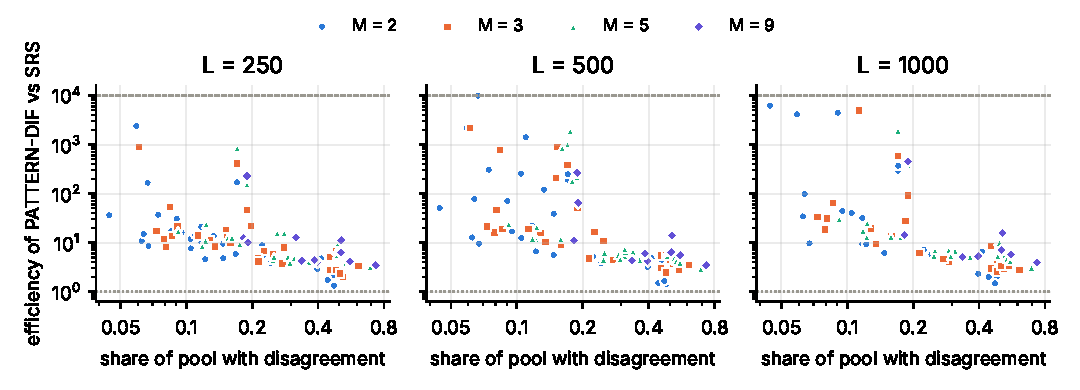
\includegraphics[width=\textwidth]{figures/abl_dif_models_disagreement.pdf}
\caption{Efficiency of PATTERN-DIF relative to SRS (median over targets) against the share of the pool on which the compared models do not all agree, for random subsets of $M$ models in every setting (A3). Both axes are logarithmic; the dotted line marks parity and the dashed line the clipping value $10^4$.}
\label{fig:abl-models}
\end{figure}

\subsection{Small-sample inference (A4)}

With the plain estimator the main study found worst-target coverage near 0.5 at $L=250$ in Churn and Law school, traced to strata whose sampled units show no variation in the influence values. The difference estimator removes most of this: the residual $\xi_i=t_i-\psi_i=(Y_i-\pi_i)(u_i-v_i)$ varies even when no positive is sampled, no (replication, target) pair had a standard error of exactly zero (plain estimator: up to 1.0\% in Law school), and the worst-target Wald coverage in Churn at $L=250$ rises from 0.47 to 0.91 (Table~\Mref{tab:abl-inference}, Figure~\ref{fig:abl-coverage}). The shortfalls that remain are of a different kind. Over the 29 cells the worst-target Wald coverage is below 0.85 in five cells (Law school 0.63, MAGIC 0.78 and Adult-sex 0.82 at $L=250$, Bank 0.83 and Phoneme 0.83 at $L=500$), against five cells for HT and six for SRS-DIF. The worst target is a TPR contrast in 17 of 29 cells (FPR in 4, error difference in 8). On average over cells its mean standard error is 0.90 of the Monte Carlo standard deviation (0.99 for the median target) and its bias is below 0.16 standard deviations, so the intervals are too short rather than off-centre, which is consistent with a linearisation error in a ratio with few sampled positives in the smaller group (we did not test this further).

None of the standard corrections closes this gap. A $t$ quantile with \citet{satterthwaite1946} degrees of freedom adds 1\% to the width and moves the mean worst target at $L=250$ from 0.852 to 0.865. The stratified bootstrap percentile interval \citep{efron1979}, which resamples labelled residuals within strata ($B=999$, no finite-population correction; \citealt{raowu1988} discuss a rescaled version), is 11\% wider and a little conservative (mean coverage 0.961 over all cells), with worst target 0.878 and minimum 0.767. The proxy variance floor of \texttt{tcs.labeling\_dif} replaces the sample variance of a stratum by its proxy residual variance when the former is exactly zero ('zero') or by the larger of the two in every stratum ('max'). The 'zero' floor leaves the width unchanged (1.002) and lifts the minimum over cells from 0.633 to 0.780, entirely through Law school (0.90 at $L=250$); combined with the $t$ quantile the mean worst target is 0.885 and four cells stay below 0.85. Only the 'max' floor reaches 0.92 in every cell (mean worst target 0.948), and it is conservative: mean coverage 0.985 at $L=250$, width 1.67 times Wald on average, 1.25 in the median and 4.9 in Law school. For SRS-DIF Wald coverage is poor (minimum 0.27) and the bootstrap worse (0.10); 'max' repairs it (minimum 0.88) at 23\% extra width. The floors were designed after seeing the failure of the plain estimator on these pools, so the 'zero' result for Law school is in-sample (the residual floor is discussed further in Section~\ref{sec:simulation}). An independent check on synthetic pools (\texttt{results/floor\_check.json}) found that the floor leaves the interval width unchanged (median ratio 1.00).

\begin{figure}[t]
\centering
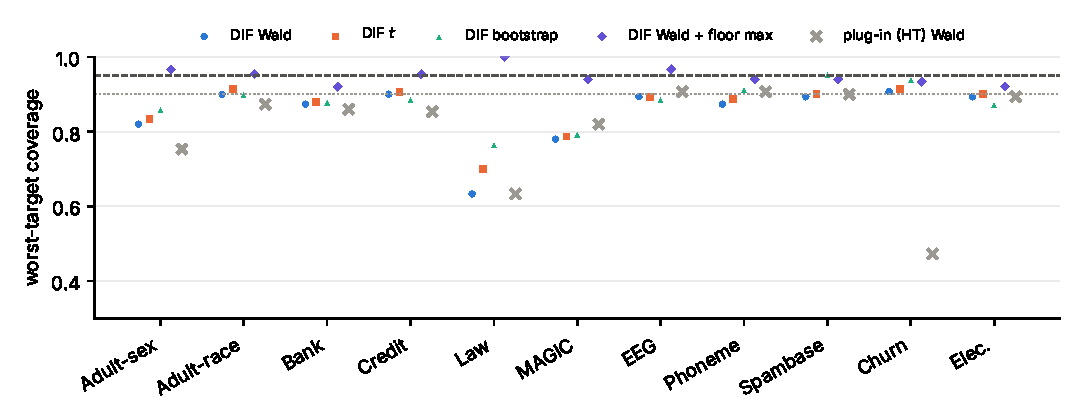
\includegraphics[width=\textwidth]{figures/abl_dif_coverage_L250.pdf}
\caption{Worst-target coverage at $L=250$ in each setting for PATTERN-DIF under four interval methods and for the plain estimator (A4). Dashed line: nominal 0.95; dotted line: expected minimum over 108 targets of 150-replicate coverage if every target covered exactly 95\% (0.90; Law school has 57 targets).}
\label{fig:abl-coverage}
\end{figure}

\subsection{Ranking models by the equalised-odds gap (A5)}

Practitioners also look at each model's equalised-odds gap $EO_m=\max(|\Delta^{TPR}_m|,|\Delta^{FPR}_m|)$ \citep{hardt2016} and rank models by it. We computed the plug-in $\widehat{EO}_m=f_{EO}(\hat T)$ from the totals of the same samples, with the difference estimator (DIF totals) and the plain estimator, and recorded the RMSE, the probability $P$ that the model with the smallest estimated gap has the smallest true gap, Kendall's $\tau$ \citep{kendall1938} between estimated and true gaps, and the bias. We also include a variant of PATTERN whose allocation targets the $2M$ per-model gaps instead of the comparison contrasts (gap-targeted). Table~\ref{tab:abl-eo} summarises the results; per-cell values are in Table~\ref{tab:abl-app-eo}.

The plug-in $\widehat{EO}_m$ is biased upwards, as a maximum of absolute values must be (mean bias 0.042 for SRS, 0.026 for PATTERN with HT, 0.024 for PATTERN-DIF, 0.019 for the gap-targeted variant with DIF). PATTERN-DIF is more accurate than SRS in the median (efficiency 1.94 to 2.21) and identifies the best model more often (mean $P$ 0.50 against 0.35 at $L=250$; 0.46 against 0.21 without Law school, where six models tie, and EEG, where the best model leads by 0.039). PATTERN with HT reaches efficiency 1.80 to 1.94 and $P$ 0.46 to 0.62, so the difference estimator adds little for this purpose. The gain is not uniform: PATTERN-DIF is less accurate than SRS in all Electricity cells (0.57 to 0.73) and in MAGIC at $L=1000$, because the allocation spends labels on disagreement whereas the gap of one model depends on all of its positive predictions. SRS-DIF has about the same RMSE efficiency (2.08 to 2.28) but a lower $P$ (0.42 at $L=250$) and $\tau$ (0.41). The gap-targeted allocation with the difference estimator is the best design here (efficiency 2.30 to 2.61, $P=0.49$, 0.56, 0.65 and $\tau=0.48$, 0.54, 0.64 by budget; never worse than SRS except in Law school) but it keeps only 74\% of the precision for the comparison contrasts (Table~\Mref{tab:abl-design}). In Law school the models are near-perfect and six have $EO_m=0$ exactly; the plain estimator then returns exactly zero for them and wins every tie, whereas the difference estimator does not (MSE ratio clipped at $10^{-4}$). When the true margin to the next model is 0.002 or less (Adult-sex, Bank, Credit card default, Churn) identification is hard for every design: $P$ for PATTERN-DIF is at most 0.55 at the largest budget and 0.11 in Credit card default (margin 0.0003).

\begin{table}[t]
\centering\footnotesize
\setlength{\tabcolsep}{4pt}
\caption{Equalised-odds gap (A5). Eff.: median over cells of the median over models of $\mathrm{MSE}_{\mathrm{SRS}}/\mathrm{MSE}$ for $\widehat{EO}_m$ (cells in which both are exactly zero are skipped); $P$: mean probability that the estimated smallest-gap model has the smallest true gap; $\tau$: mean Kendall $\tau$ between estimated and true $EO_m$. DIF: totals from the difference estimator; plug-in: plain estimator.}
\label{tab:abl-eo}
\begin{tabular}{lccccccccc}
\toprule
 & \multicolumn{3}{c}{$L=250$} & \multicolumn{3}{c}{$L=500$} & \multicolumn{3}{c}{$L=1000$} \\
\cmidrule(lr){2-4}\cmidrule(lr){5-7}\cmidrule(lr){8-10}
Design & Eff. & $P$ & $\tau$ & Eff. & $P$ & $\tau$ & Eff. & $P$ & $\tau$ \\
\midrule
SRS (plug-in) & 1.00 & 0.35 & 0.32 & 1.00 & 0.42 & 0.39 & 1.00 & 0.49 & 0.48 \\
SRS-DIF (PPI) & 2.08 & 0.42 & 0.41 & 2.22 & 0.47 & 0.45 & 2.28 & 0.53 & 0.55 \\
GROUP, plug-in & 1.07 & 0.37 & 0.34 & 1.10 & 0.43 & 0.42 & 1.63 & 0.51 & 0.52 \\
PATTERN, plug-in (HT) & 1.83 & 0.46 & 0.45 & 1.80 & 0.51 & 0.49 & 1.94 & 0.62 & 0.62 \\
PATTERN-DIF (default) & 1.94 & 0.50 & 0.48 & 1.94 & 0.53 & 0.51 & 2.21 & 0.61 & 0.62 \\
Gap-targeted, plug-in & 2.03 & 0.44 & 0.43 & 2.29 & 0.52 & 0.51 & 2.54 & 0.59 & 0.61 \\
Gap-targeted, DIF & 2.30 & 0.49 & 0.48 & 2.61 & 0.56 & 0.54 & 2.51 & 0.65 & 0.64 \\
ORACLE-ALLOC, DIF & 2.02 & 0.50 & 0.47 & 1.77 & 0.54 & 0.52 & 1.93 & 0.57 & 0.60 \\
\bottomrule
\end{tabular}

\end{table}

\paragraph{Summary.} With the difference estimator the ablation conclusions about the design are those of the earlier plug-in study: the count $K_i$ is the stratifier worth having, Neyman rather than proportional allocation matters, the allocation is insensitive to the proxy, and the gain depends on how often the compared models disagree. Three things differ. First, the proxy now matters in the estimator, where a poor proxy costs up to half of the efficiency and removes the advantage over HT, although coverage is unaffected; the ensemble mean was never beaten there. Second, the difference estimator removes the zero-variance failure of the plain estimator, so the proxy variance floor has become a cheap safeguard ('zero', no loss of width) rather than a 19\% widening, and the remaining undercoverage of rate contrasts at $L=250$ is not fixed by $t$ quantiles, the bootstrap or the floor; only the conservative 'max' floor reaches nominal worst-target coverage. Third, for ranking models by $EO_m$ itself the gap-targeted allocation with the difference estimator is better than the default. Neither tuned $\lambda$ nor proxy-bin strata beat the default consistently, and we keep it; we recommend reporting the Wald interval with the 'zero' floor, which costs nothing in width.

% appendix_ablations (to be written)

% appendix_data (to be written)

\end{document}
